\documentclass[doctor]{iscs-thesis}

%\usepackage{cleverref}
\usepackage{stmaryrd,setspace,float}
\usepackage[counterclockwise]{rotating}
\usepackage{enumitem}
\usepackage{textcomp}
\usepackage{makeidx}

\makeindex

%% from http://yav.purely-functional.net/haskell_latex.html
\usepackage{fancyvrb}
\DefineVerbatimEnvironment{code}{Verbatim}{fontsize=\small}
\DefineVerbatimEnvironment{spec}{Verbatim}{fontsize=\small}
\newcommand{\ignore}[1]{}

\def\NAT@spacechar{~}% NEW

\usepackage{rotating}

\usepackage{bussproofs,stmaryrd, showlabels}
\EnableBpAbbreviations
\usepackage{graphicx}	% required for `\includegraphics' (yatex added)
\usepackage[numbers,sort&compress]{natbib}

%%% from haskell symposium submitted paper
\usepackage{graphicx}
\usepackage{bussproofs}
\usepackage{amsmath,amssymb}

\usepackage[amsmath,standard,thref]{ntheorem}
%\usepackage{showlabels}

% \doublespacing

\newcommand{\Nat}{{\mathbb N}}
\newcommand{\Real}{{\mathbb R}}
\newcommand{\pvar}{\mathsf{PVar}}
\newcommand{\agents}{\mathcal A}
\newcommand{\wvar}{\mathsf{WVar}}

\newcommand{\tuple}[1]{\langle{#1}\rangle}
\newcommand{\fix}[1]{[FIX \fbox{#1}]}
\newcommand{\fml}{\mathsf{\operatorname{Fml}}}
\newcommand{\id}{\operatorname{id}}
\newcommand{\kv}{$\mathbf K \vee$}
\newcommand{\vdashR}{\vdash_{\mathsf R}}

\newcommand{\vdashRLB}{\vdashR^{\mbox{\tiny \LB}}}

\newcommand{\T}{\mathbf T}
\newcommand{\memory}{{\sf m}}
\newcommand{\ruleskip}{\vskip 5mm}

%%%

\newcommand{\R}[1]{{#1}^{\mathsf R}}
\newcommand{\modelsR}{\models_{\mathsf R}}


\newtheorem{notation}{Notation}

\newcommand{\nat}{\mathbb{N}}
\newcommand{\steps}[2]{Steps_{#1}\left({#2}\right)}

\newcommand{\hypc}[2]{{\mathcal{C}#1}\left[{#2}\right]}
\newcommand{\hyper}{\mathcal{H}}
\newcommand{\hypert}{\mathcal{O}}
\newcommand{\hmid}{\ \ \rule[-2pt]{2pt}{9pt}\ \ }

\newcommand{\tr}{\vdash}
\newcommand{\update}{\vartriangleleft}

\newcommand{\elim}{\mathcal E}
\newcommand{\intro}{\mathcal I}

\newcommand{\coml}{\leftarrow_{\mathrm g}}
\newcommand{\comr}{\leftarrow_{\mathrm d}}

\newcommand{\reduce}{\rightsquigarrow}
\newcommand{\reduction}{\reduce^\ast}
\newcommand{\processes}{\mathbb{P}}
\newcommand{\ProV}{\mathsf{ProV}}
\newcommand{\LB}{\textbf{LB}}
\newcommand{\p}[1]{\texttt{#1}}

%% terms
\newcommand{\lpair} [1]{\langle{#1}\rangle}
\newcommand{\cotuple}[1]{[{#1}]}
\newcommand{\ev}[1]{\mathsf{ev}\left({#1}\right)}

\newcommand{\inl}[1]{\mathsf{inl}({#1})}
\newcommand{\inr}[1]{\mathsf{inr}({#1})}

\newcommand{\linl}[1]{\mathsf{inl}\left({#1}\right)}
\newcommand{\linr}[1]{\mathsf{inr}\left({#1}\right)}

\newcommand{\lpil}[1]{\pi_{\mathsf l}\left({#1}\right)}
\newcommand{\lpir}[1]{\pi_{\mathsf r}\left({#1}\right)}

\newcommand{\mats}[6]{\langle \inl{#1}. ({#2},{#3})/ \inr{#4}. ({#5},{#6})\rangle}
\newcommand{\mat} [5]{\mathsf{match}\,{#1}\,\mathsf{of}\, \inl{#2}. {#3}/
\inr{#4}. {#5}}

\newcommand{\ifte}[3]{\mathsf{If}\, {#1}\, \mathsf{then}\, {#2}\,
\mathsf{else}\, {#3}}

\newcommand{\abort}{\mathsf{abort\,}}

\newcommand{\compare}[2]{{#1} == {#2}}

\newcommand{\term} [0]{M}
\newcommand{\lterm}[0]{\mathcal{T}^-}
\newcommand{\val}  [0]{\mathcal{V}}
\newcommand{\lval} [0]{\mathcal{V}^-}
\newcommand{\tj}   [2]{ {#1} \colon{#2} }

\newcommand{\wor}{\,\mathbin{\mathsf{or}}\,}

\newcommand{\Id}{\mathsf{Id}}
\newcommand{\lgd}{$\lambda$-GD}

%% configuration
\newcommand{\lstore}{{S}}
\newcommand{\conf}[2]{(\lstore{#1},{#2})}
\newcommand{\confwithcontext}[3]{\conf{#1}{#2}{\hypert\hmid C[{{#3}}]\hmid\hypert'}}
\newcommand{\concreteconf}[2]{({#1},{#2})}

%% reductions and the like
\newcommand{\breduce}{\reduce_{\mathrm B}}
\newcommand{\areduce}{\reduce_{\mathrm A}}
\newcommand{\wreduce}{\reduce_{\mathrm W}}
\newcommand{\rreduce}{\reduce_{\mathrm R}}
\newcommand{\preduce}{\reduce_{\mathrm P}}
\newcommand{\bpreduce}{\reduce_{\mathrm{B/P}}}

%% logical rules
\newcommand{\UnaryRule}[3]{ \AxiomC{#1}
\LeftLabel{#2}
\UnaryInfC{#3} \DisplayProof}
\newcommand{\BinaryRule}[4]{ \AxiomC{#1} \AxiomC{#2}
\LeftLabel{#3}
\BinaryInfC{#4}\DisplayProof}
\newcommand{\TrinaryRule}[5]{ \AxiomC{#1} \AxiomC{#2}
\AxiomC{#3} \LeftLabel{#4}
\TrinaryInfC{#5} \DisplayProof}

%% investi
\newcommand{\inv}[1]{{#1}^{\mathsf i}}

\newcommand{\rightlocal}{\rightsquigarrow_{\beta{\mathrm l}}}
\newcommand{\rightcomm}{\rightsquigarrow_{\beta{\mathrm c}}}
\newcommand{\rightdist}{\rightsquigarrow_{\beta{\mathrm d}}}
\newcommand{\dist}[2]{[{#1}; {#2}]}

\newcommand{\interpret}[1]{\llbracket {#1} \rrbracket}

\newcommand{\process}{p}
\newcommand{\contex}[1]{\mathcal C[{#1}]}
\newcommand{\semo}[1]{\llbracket{#1}\rrbracket}
\newcommand{\semoi}[1]{\llparenthesis{#1}\rrparenthesis}
\newcommand{\semi}[1]{\llparenthesis{#1}\rrparenthesis}

\newcommand{\wwedge}{\operatorname*{\bigwedge\kern -8pt \bigwedge}}

% macros
\newcommand {\G}{\Gamma}
\newcommand {\D}{\Delta}

\renewcommand{\phi}{\varphi}
\newcommand{\imp}{\supset}

\newcommand{\bbot}{
    \mathord{\reflectbox{\rotatebox[origin=c]{-90}{$\models$}}}}

\newcommand{\form}{\mathop{\text{Form}}}

\newcommand{\ruleT}[1]{\LeftLabel{(T)}\UnaryInfC{${#1}$}}
\newcommand{\powerset}[1]{{\mathcal P({#1})}}
\newcommand{\proj}[0]{\operatorname{proj}}
\newcommand{\len}[0]{\operatorname{len}}
\newcommand{\cl}[0]{\operatorname{cl}}
\newcommand{\carrier}[0]{\operatorname{carrier}}
\newcommand{\subfml}{\operatorname{subfml}}
\newcommand{\seq}{\operatorname{Seq}}
\newcommand{\type}{\operatorname{Type}}
\newcommand{\vdashsc}{\vdash_{\mbox{\rm sc}}}
\newcommand{\iec}{{\rm {\textbf{IEC}}}}
\newcommand{\ckv}{{\rm {\textbf{S4}\ast\cdots\ast\textbf{S4}}}}
\newcommand{\vdashsf}{\vdash_{\ckv}}
\newcommand{\initial}[1]{${#1}\vdashn{#1}$}
\newcommand{\supsete}[1]{\LeftLabel{($\supset$-E)}\BinaryInfC{${#1}$}}
\newcommand{\supseti}[1]{\LeftLabel{($\supset$-I)}\UnaryInfC{${#1}$}}
\newcommand{\nec}[1]{\LeftLabel{(nec)}\UnaryInfC{${#1}$}}
\newcommand{\wedgeel}[1]{\LeftLabel{($\wedge$-E$_0$)}\UnaryInfC{${#1}$}}
\newcommand{\wedgei}[1]{\LeftLabel{($\wedge$-I)}\BinaryInfC{${#1}$}}
\newcommand{\veeil}[1]{\LeftLabel{($\vee$-I$_0$)}\UnaryInfC{${#1}$}}
\newcommand{\veeir}[1]{\LeftLabel{($\vee$-I$_1$)}\UnaryInfC{${#1}$}}
\newcommand{\veee}[1]{\LeftLabel{($\vee$-E)}\TrinaryInfC{${#1}$}}
\newcommand{\weaken}[1]{\LeftLabel{(w)}\UnaryInfC{${#1}$}}
\newcommand{\be}[1]{\LeftLabel{($\bot$-E)}\UnaryInfC{${#1}$}}
\newcommand{\ax}[1]{	     \AxiomC{}
	     \LeftLabel{(ax)}
\UnaryInfC{\initial{#1}}}
\newcommand{\dn}[1]{\LeftLabel{(DN)}\UnaryInfC{${#1}$}}

\newcommand{\xphi}{\tj{x}{\phi}}
\newcommand{\ypsi}{\tj{y}{\psi}}

\newcommand{\rev}[1]{{#1}^{-1}}

\newcommand{\sem}[1]{|{#1}|}
\newcommand{\nsem}[1]{\sem{#1}^-}
\newcommand{\sempair}[1]{\sem{(#1)}}

\renewcommand{\vec}{\overrightarrow}
\newcommand{\sche}{\sqsubseteq}


\newcommand{\sequent}[2]{{#1}\tr{#2}}
\newcommand{\aseq}[2]{\AxiomC{$\sequent{#1}{#2}$}}
\newcommand{\useq}[2]{\UnaryInfC{$\sequent{#1}{#2}$}}
\newcommand{\bseq}[2]{\BinaryInfC{$\sequent{#1}{#2}$}}
\newcommand{\tseq}[2]{\TrinaryInfC{$\sequent{#1}{#2}$}}

\newcommand{\limp}{\multimap}

\newcommand{\conc}{\parallel}
\newcommand{\comod}[2]{\ast^{\rightarrow {#2}}_{\leftarrow{#1}}}
\newcommand{\reader}[1]{\ast_{\leftarrow{#1}}}

\newcommand{\sred}{\succ_{\mathsf s}}
\newcommand{\ared}{\succ_{\mathsf a}}
\newcommand{\red}{\succ}

\newcommand{\comodL}{\comod c{\co c}}
\newcommand{\comodR}{\comod{\co c}{c}}

\newcommand{\sLambda}{\Lambda_{\mathsf s}}
\newcommand{\aLambda}{\Lambda_{\mathsf a}}
\newcommand{\sPi}{\Pi_{\mathsf s}}
\newcommand{\aPi}{\Pi_{\mathsf a}}
\newcommand{\FLe}{FL$_{\mathrm {e}}$}
\newcommand{\MTLs}{MTL$_{\mathrm{s}}$}
\newcommand{\bu}[1]{{#1}^\bullet}
\newcommand{\HLBCK}{\mathbf{HL}^\forall_{\mathbf{BCK}}}

\newcommand{\NMTL}{\mathbf{N}_{\mathbf{MTL2}}}
\newcommand{\NMLL}{\mathbf{N}_{\mathbf{IMLL2}}}

\newcommand{\eH}{e_{\hatma H}}
\newcommand{\eI}{e_{\hatma I}}
\newcommand{\hatma}[1]{\hat{\mathcal{#1}}}
\newcommand{\takehyper}[1]{e_{#1}\in \semo{#1}}
\newcommand{\eHz}{e_{\mathrm{H0}}}
\newcommand{\eHo}{e_{\mathrm{H1}}}

\newcommand{\co}[1]{\bar{#1}}

\newcommand{\letpar}[4]{\mathsf{let}\, {#1} \,\mathsf{be}\, ({#2}\conc
{#3})\, \mathsf{in}\, {#4}}

\newcommand{\brac}[1]{\lbrack {#1}\rbrack}

\newcommand{\imapsto}[1]{\{i\mapsto {#1}\}}
\newcommand{\kmapsto}[1]{\{k\mapsto {#1}\}}
\newcommand{\mmapsto}[1]{\{m\mapsto {#1}\}}
\newcommand{\jmapsto}[1]{\{j\mapsto {#1}\}}

\newcommand{\bool}{\mathbb{B}}

\newcommand{\dom}{\mathop{\mathrm{dom}}}
\etitle{A Computational Interpretation of G\"odel--Dummett Logic}
\jtitle{$B%2!<%G%k!&%@%a%C%HO@M}$N7W;;E*2r<a(B}
\eauthor{Yoichi Hirai}
\jauthor{$BJ?0fMN0l(B}
\esupervisor{Masami Hagiya}
\jsupervisor{$BGkC+>;8J(B}
\supervisortitle{Professor} % Professor, etc.
\date{\fix{XXX}}

\begin{document}

\begin{eabstract}
 We propose hyper-lambda calculi, the typed lambda calculi based on
 hypersequent calculi.  A hyper-lambda term is a finite
 sequence of lambda terms, which represent concurrent processes.  We give
 three concrete hyper-lambda calculi: one synchronous and the other two
 asynchronous.  All
 employ a
 pair of communication primitives exchanging their inputs.
 In the synchronous case, both sides succeed.  In the asynchronous cases,
 at least one side obtains the other side's input.
 The synchronous calculus implements message-passing communication
 and session types;
 the asynchronous calculus characterizes shared-memory waitfree
 communication.
 Among processes of a typed hyper-lambda term,
 all succeed in the synchronous case while
 at least one succeeds in the asynchronous case.
 Logically, the processes are interpreted conjunctively
 in the synchronous case but disjunctively in the asynchronous case.
 The synchronous calculus is based on Abelian logic:
 $(\phi\limp\psi)\otimes(\psi\limp\phi)$ on top of multiplicative
 additive fragment of intuitionistic linear
 logic (without some units);
 one of the asynchronous calculi is based on G\"odel-Dummett logic:
 $(\phi\imp\psi)\lor(\psi\imp\phi)$ on top of intuitionistic logic.
 The hyper-lambda calculi are in Curry-Howard correspondence with the
 deduction systems for these logics.
 We also give a similar development monoidal t-norm logic and
 implement the G\"odel-Dummett case using Haskell.
\end{eabstract}

\begin{jabstract}
 $B%O%$%Q!<%i%`%@7W;;$9$J$o$A%O%$%Q!<?d7o7W;;$K4p$E$/7?IU$-%i%`%@7W;;$rDs0F$9$k!%(B
 $B%O%$%Q!<%i%`%@9`$O%i%`%@9`$NM-8BNs$G!$JBNs%W%m%;%9$rI=$9!%(B
 $BF14|$HHsF14|$HFs$D$N%O%$%Q!<%i%`%@7W;;$rM?$($k!%(B
 $BN><T$H$b$K!$8_$$$KF~NO$r8r49$9$kDL?.;R$NBP$rMQ$$$k!%(B
 $BF14|%O%$%Q!<%i%`%@7W;;$G$O!$DL?.;RAPJ}$,@.8y$9$k!%(B
 $BHsF14|%O%$%Q!<%i%`%@7W;;$G$O!$DL?.;R$N>/$/$H$bJRJ}$,$b$&JRJ}$NF~NO$r3MF@(B
 $B$9$k!%(B
 $BF14|%O%$%Q!<%i%`%@7W;;$O%a%C%;!<%8%Q%C%7%s%0DL?.$H%;%C%7%g%s7?$r<BAu$7!$(B
 $BHsF14|%O%$%Q!<%i%`%@7W;;$O6&M-%a%b%j$NL5BT5!7W;;$rFCD'$E$1$k!%(B
 $B7?IU$-%O%$%Q!<%i%`%@9`$N%W%m%;%9$I$b$N$&$A!$F14|%O%$%Q!<%i%`%@7W;;$G$OA4(B
 $B$F$,@.8y$9$k$,!$HsF14|%O%$%Q!<%i%`%@7W;;$G$O>/$/$H$b0l$D$,@.8y$9$k!%(B
 $BO@M}E*$K%W%m%;%9$I$b$O!$F14|%O%$%Q!<%i%`%@7W;;$G$OO"8@$G!$(B
 $BHsF14|%O%$%Q!<%i%`%@7W;;$G$OA*8@$G2r<a$5$l$k!%(B
 $BF14|%O%$%Q!<%i%`%@7W;;$O%"!<%Y%kO@M}$K4p$E$/(B: $BD>4Q<g5A@~7AO@M}(B
 $B$N>hK!E*2CK!E*CGJR(B($B=|$$$/$D$+$NC10LO@M}<0(B)$B$K8xM}(B
 $(\phi\limp\psi)\otimes(\psi\limp\phi)$$B$r2C$($?(B
 $BO@M}$G$"$k!%HsF14|%O%$%Q!<%i%`%@7W;;$O%2!<%G%k!&%@%a%C%HO@M}$K4p$E$/(B:
 $BD>4Q<g5AO@M}$K8xM}(B$(\phi\imp\psi)\lor(\psi\imp\phi)$$B$r2C$($?O@M}$G$"$k!%(B
 $B$3$l$i$N%O%$%Q!<%i%`%@7W;;$O!$$=$l$>$l$NO@M}$N1iehBN7O$H%+%j!<!&%O%o!<(B
 $B%IBP1~$K$"$k!%(BMonoidal t-norm$BO@M}$K4p$E$/JQ<o$H!$(BHaskell$B$rMQ$$$?<BAu$b07$&!%(B
\end{jabstract}


\maketitle

\begin{acknowledge}
 I thank my adviser Masami Hagiya for his patience and some decisive
 comments at important moments.
 Even before composing this thesis, I became indebted to many of the
 juries and their colleagues.
 In an MLG (methematical logic group) meeting, Hiroakira Ono asked me
 about the constructive content of Dummett axiom, which I answer in
 Chapter~\ref{ch:lambda}.
 Naoki Kobayashi's request for a stronger communication primitive
 resulted in Chapter~\ref{ch:exchange}.
 Ichiro Hasuo gave me some chances of talks and
 indispensable advice on visiting the Netherland
 and studying there.
 As well as by other juries,
 I await valuable comments by Shinichi Honiden and Andrzej Murawski from
 practical and theoretical viewpoints.

 The work about hyper-lambda calculus is encouraged by feedbacks from
 ACAN (Algebraic and Coalgebraic Approaches to
 Non-Classical Logics Workshop) and OPLSS'11 participants,
 Pisa Proof Theory Workshop, FLOPS-2012
 and numerous other occasions.

 Grant-in-Aid for JSPS Fellows 23-6978 supported
 my second and third years of PhD, of which almost one year was spent
 in ILPS, the University of Amsterdam.
 The author thanks Maarten Marx, Maarten de Rijke and other members of ILPS for
 comfortable environments and stimulating discussions during my stay.
 Especially, working on heavy problems for months with Maarten Marx, Alessandro
 Facchini and Evgeny Sherkhonov was a unique training.

 The author thanks Tadeusz Litak for encouragements and
 information on relevant research.
 At the University of Tokyo,
 discussions with Tatsuya Abe, Yoshihiko Kakutani and Masahiro Hamano
 nurtured my taste on formalistic, semantic and graphical approaches.
\end{acknowledge}


\frontmatter
\tableofcontents

\listoffigures

\newpage
\chapter*{List of Theorems}
\theoremlisttype{allname}
\listtheorems{theorem,lemma}
% XXX because empty %\listoftables

\mainmatter

\chapter{Introduction}

\subsection{Our Contributions}

We propose hyper-lambda calculi.
Instead of lambda terms in ordinary lambda calculi,
we use a finite sequence of lambda terms called hyper-lambda terms.
We give two such examples:
one models synchronous send--receive communication (Chapter~\ref{ch:exchange}) and
the other models asynchronous waitfree
read--write communication (Chapter~\ref{ch:lambda}).
We also give an example of hyper-lambda calculi style programming in Haskell.
The two hyper-lambda calculi are in Curry--Howard correspondence with
hypersequent formulation of logics: Amida logic and G\"odel--Dummett
logic.
G\"odel--Dummett logic is an intermediate logic.
An intermediate logic is a logic \textit{between} classical and
intuitionistic logics, where `between' is defined using the
set-theoretic inclusion of valid logical formulae of each logic.
Amida logic is a substructural logic.

\citet{hosoi-ono} declared that they chose to study intermediate
logics in
general rather than studying specific intermediate logics.
However, concrete results about specific subjects matter when the
results contain new phenomena.
This thesis is intended to contain such concrete discoveries
about specific intermediate and substructural logics.

The famous logic among th two,
G\"odel--Dummett logic, is
a typical intermediate logic logic known from 1950's.
Our method is the Curry--Howard correspondence, also known from 1940's.
Our result is characterization of waitfreedom, a concept in the theory
of distributed computation extensively studied in 1990's.
Since both sides of the correspondence is already known,
the discovery is a replay of Curry's surprise.

Of course, there have been many instances of Curry--Howard correspondence.

We list our contributions from the most important:
\begin{enumerate}
 \item developing a lambda calculus using
       a hypersequent calculus (Chapters~\ref{ch:lambda,ch:exchange});
 \item identifying the computational ability of the
       G\"odel--Dummett logic with waitfreedom (Chapter~\ref{ch:lambda});
 \item encoding session types using a seemingly unknown axiom
       $(p\limp q)\otimes(q\limp p)$ (which we call Amida axiom) on top
       of intuitionistic linear logic (Chapter~\ref{ch:exchange}),
 \item discovery of Amida logic (Chapter~\ref{ch:exchange});
 \item using conjunctive hypersequents for the first time (Chapter~\ref{ch:exchange}).
\end{enumerate}

Our first contribution is the technique for our first contribution.
We developed a lambda calculus based on \citet{avron91}'s hypersequents.
\citet{avron91} himself noted that it would be important to develop a
lambda calculus for hypersequents.
The lambda calculus relies on \citet{avron91}'s hypersequents.
The hypersequent calculus is a
variant of the deduction system called sequent calculus.  In sequent
calculus, each step of a proof tree concludes a sequent $\G\vdash\phi$ that
consists of a finite sequence of logical formulae~$\G$ and a logical
formula~$\phi$.  The sequent $\G\vdash\phi$ is
interpreted as an implication.  In hypersequent calculus, each step of a
proof tree concludes a hypersequent instead of a sequent.  A
hypersequent is a sequence of sequents delimited by $\hmid$:
$\G\vdash\phi\hmid \D\vdash\psi
\hmid \cdots$.  Also here, each component is interpreted as an
implication, and then the whole hypersequent is interpreted as the
disjunction of all those implications.
When we interpret proofs as programs, we take the components as
concurrent processeses.  Following the original disjunctive
interpretation of components, we regard the proof tree as the guarantee of
success of at least one process.

Our second contribution is finding a way to interpret proofs in
G\"odel--Dummett logic as
concurrently executable programs for waitfree computation.
Although \citet{avron91} noticed his hypersequent calculus has something
to do with concurrency (as the title of~\citep{avron91} contains the phrase
``intermediate logics for concurrency''), it was unknown that
the computational interpretation of G\"odel--Dummett logic has
the degree of synchronization called waitfreedom.  This discovery
constitutes our first contribution.

According to \citet[p.97]{curryhoward},
the Curry--Howard isomorphism~\citep{curryhoward} was first made
precise by \citet[\textbf{9}E and
\textbf{9}F]{curry1974combinatory}.
The intuitionistic propositional logic and the typed lambda calculus
had been independently invented but Curry discovered them to be the same thing.
The ``double discovery'' (\citet{wadler2012propositions}) is considered
to affirm the importance of the typed lambda calculi.
In this thesis we witness a replay of the ``double discovery'' with
different casts: G\"odel--Dummett logic and the waitfreedom.
Both of these were born in the early eras of their respective academic
disciplines:
mathematical logic bore G\"odel Dummett logic in
1950's~\citep{dummett59}
and the computer science bore waitfree computation in
1970's~\citep{lamport1979make}.
Chapter~\ref{ch:exchange} is about the unknown connection between these two.

This is the first such computational
interpretation for intermediate logics (Fig.~\ref{fig:lattice}).
Another significance of this contribution
is giving interpretation of nondterminism in typed
lambda calculi.  In the simply typed lambda calculus for intuitionistic
propositional logic, all typed terms have a unique normal form.
However, in typed lambda calculi for classical propositional logic,
there can be multiple normal forms unless we employ an evaluation
strategy or limit the set of reductions.
The lack of unique normal forms in the classical propositional proofs
has puzzled logicians for decades. \fix{mention Lafont's example; say it
is a matter of concurrency}
 \begin{figure}
  \centering
  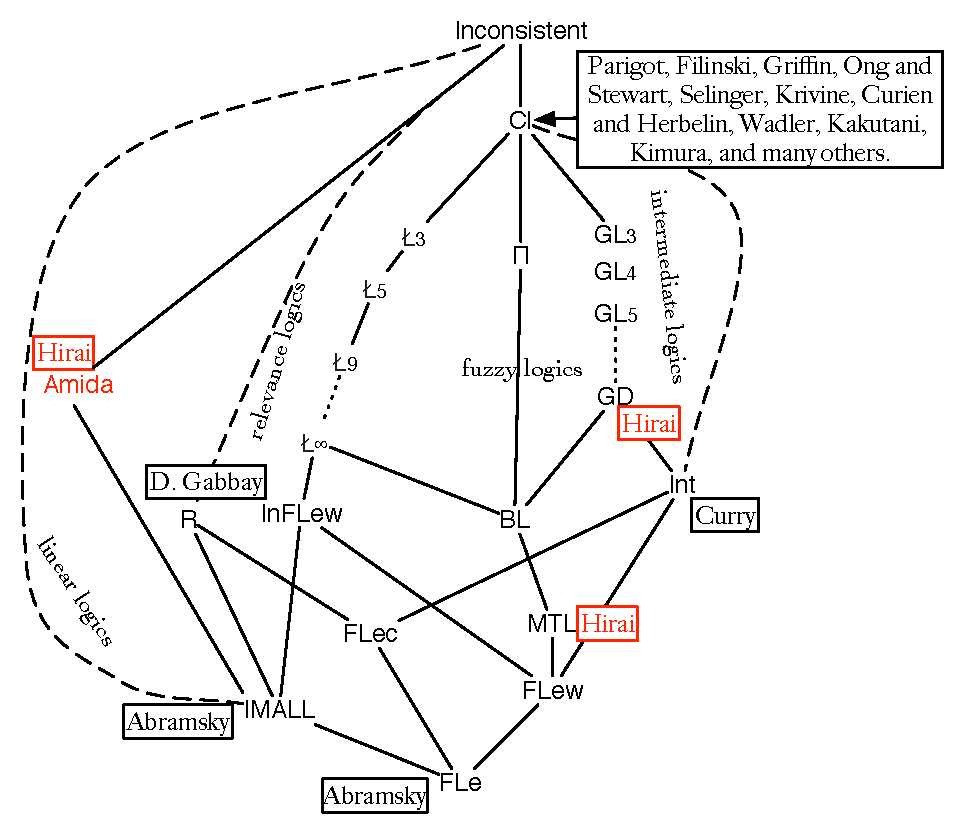
\includegraphics[scale=0.8]{lattice.eps}
  \caption[The lattice of substructural logics, some of which with known lambda calculi.]
  {The substructural logics for which lambda calculi are found.
  The underlying Hasse diagram of well-known substructural logics is
  taken from
  \cite[p.~120]{residuated} with slight modifications.
  The names in boxes refer to people who developed lambda calculi for
  these logics.
  \textsf{GD} stands for G\"odel--Dummett logic, for which
  a lambda calculus will be given in
  Chapter~\ref{ch:lambda}.
  \textsf{Amida} stands for the Amida logic, an original logic
  defined in Chapter~\ref{ch:exchange}.
  \textsf{MTL} stands for monoidal t-norm logic~\citep{Esteva2001271},
  for which a lambda calculus will be given
  in Chapter~\ref{ch:pole}.
  \textsf{FLe} is for the full Lambek calculus with exchange
  rule~\citep[p.86]{residuated}, which is also known as the
  intuitionistic
  multiplicative additive fragment of linear logic (IMALL).
  \textsf{MALL} stands for its classical version, the multiplicative
  additive fragment of linear logic.  For these fragments of linear
  logic,
  \citet{abramsky1993computational} gave lambda calculi.
  \textsf{FLew} stands for the full Lambek calculus with exchange and
  weakening,
  which is also known as intuitionistic affine logic.
  Affine logics lack contraction, which causes exponential size increase
  during cut-elimination process.
  Asperti gave light affine logic~\citep{2002}.
  \citet{terui2007} gave an affine typed lambda calculus for polynomial
  time computation.
  \textsf{R} stands for relevance logic~\citep{urquhart1972},
  for which \citet{gabbay1992} gave a lambda calculus.
  \textsf{Int} stands for the intuitionistic propositional logic.
  The original Curry--Howard isomorphism was found for this logic by
  Curry~\citep{curry1942}.
  \textsf{Cl} stands for the classical propositional logic.
  There is intensive research going on for the computational
  interpretation of classical logic.  Namely,
  Parigot's $\lambda\mu$-calculus~\citep{lambdamu},
  Filinski's symmetric lambda calculus~\citep{filinski1989},
  Griffin's control perator~$\mathcal C$~\citep{griffin1990},
  Ong and Stewart's $\lambda\mu_{\mathrm
  v}$~\citep{ong-stewart},
%   \citet{bb1994}, this is predicate logic
  Selinger's categorical semantics and duality
  result~\citep{selinger2001} for which \citet{kakutani2002} introduced
  fixed-point
  operators,
  Curien and Herbelin's $\bar\lambda\mu\tilde\mu$
  calculus~\citep{curien2000},
  Wadler's dual calculus~\citep{wadler-dual, wadler-reloaded} and so on.
  For the history of lambda calculi for classical logic,
  Daisuke Kimura's thesis~\cite{kimura} is a source of detailed
  information.
  \textsf{Inconsistent} stands for the logic of all logical formulae.
  A programming language \texttt{Haskell}, which is based on
  the typed lambda calculi, has
  an inconsistent type system.
  }
  \label{fig:lattice}
 \end{figure}
Dynamic behaviour involves time.
One simple notion of time is that of totally-ordered events where
one event happens before the other or the other before one \fix{cite something}.
This sentence is syntactically similar to Dummett's axiom that states
one proposition implies the other or the other implies one.
We investigate whether this syntactic similarity is reflected
in the dynamic semantics of logics: namely, the lambda calculi.

Our third contribution is

Our fourth contribution is

Our fifth contribution is

\fix{turn this into a table, linear or intuitionistic, conjunction or disjunction}
The previous works treated the computational interpretations of
disjunctive formulae like $(\phi\imp\psi)\lor(\psi\imp\phi)$ or
$(\phi\limp\psi)\oplus(\psi\limp\phi)$.  In this chapter, we try
replacing these disjunctions with conjunctions.
In the former case, the change renders the logic inconsistent.
If we add the axiom $(\phi\imp\psi)\land(\psi\imp\phi)$ to the
intuitionistic propositional logic,
we can prove any formula.  However in the lattar case, the change does
not make the system meaningless.
In this chapter, we treat
the axioms of the form $(\phi\limp\psi)\otimes(\psi\limp\phi)$
on top of IMLL2, the second order formulation of intuitionistic
multiplicative linear
logic.  In essence, the axiom allows two processes to wait for one
another and then exchange information.

The content of Chapter~\ref{ch:lambda} appears in
a conference paper by the author \citep{hiraiflops2012}
although we have applied substantial modifications since then.

% \section{An Introduction for Computer Scientists}

% \section{An Introduction for Proof Theorists}

% \section{An Introduction for Functional Programmers}

% \section{An Introduction for Philosophers}


 \section{Preliminaries}

  We use ``iff\index{iff}'' as an abbreviation for ``if and only if.''
  We use set-theoretic concepts such as sets, relations and functions.
  For a set~$X$, $2^X$ denotes the powerset of $X$.
   $X\setminus Y$ denotes the subset of $X$ that consists of those
   elements of $X$ that are not elements of $Y$.
   Everywhere, we consider countably infinite set of logical formulae.
   A logic\index{logic} is a set of logical formulae, thus, there are at most
   $\powerset{\mathbb N}$ different logics once the set of logical
   formulae is fixed.
   Likewise, we consider at most countably many proofs and lambda terms.

   We denote partial maps as graphs.
   For example, $\{0\mapsto M, 1\mapsto N\}$ denotes a partial map that
   maps 0 to $M$ and 1 to $N$.
   We denote by $\dom(f)$ the domain of $f$, that is,
   the set of elements that are mapped to something.
   We also denote a partial map as a sequence whose index is the domain.
   For example, $(y_i)_{i\in I}$ denotes the partial map that maps
   $i\in I$ to $y_i$.
   For partial maps whose domains are disjoint, we use $\sqcup$ to
   denote the union.
   In other words, when $f$ and $g$ have disjoint domains, $f\sqcup g$
   denotes the
   partial map that maps $x$ to $f(x)$ or $g(x)$ when one of these is
   defined, or otherwise to nothing.

  We use BNF (Backus Naur Form) for giving inductive definitions for sets
  of sequents of symbols.
 \begin{example}[An example of BNF]
  When we say we define formulae~$\phi$ by BNF:
  \[
   \phi::= \bot \mid p\mid (\phi\imp\phi)
  \]
  where $p$ is a propositional variable, we actually define a set $\Phi$
  which is the smallest set such that
  \begin{itemize}
   \item $\bot$ is in $\Phi$
   \item each propositional variable is in $\Phi$ and
   \item if $\phi$ and $\psi$ are in $\Phi$, then $(\phi\imp\psi)$ is in $\Phi$.
  \end{itemize}
  and then we declare that we call elements of $\Phi$ formulae.
 \end{example}

 We take binary operators of the symbol $\imp$ or $\limp$,
 to be right associative.  For example, $\phi\limp\psi\limp\theta$
 is interpreted as $\phi\limp(\psi\limp\theta)$.

\section{History}

We briefly review the history of mathematical logic and computer science
to the extent relevant to this thesis.
Especially, we focus on the treatments of Dummett's axiom $(a\imp
b)\lor(b\imp a)$ using the techniques in the history.
We confine ourselves to the developments of propositional logic and
ignore anything related to predicate logic or formalization of
mathematics.

\subsection{Birth of Formal Logic}

Implication is an important concept.
One treatment of implications is called the \textit{material
implication}\index{implication!material}.
The material implication can be traced back at least to
Frege's \textit{Begriffsschrift}~\citep{frege} in 1879.\index{Frege}
There, in the
section called ``conditionality,''
he begins by establishing four cases~\citep[p.~13]{frege}:
\begin{enumerate}
 \item $A$ is affirmed and $B$ is affirmed\,;
 \item $A$ is affirmed and $B$ is denied\,;
 \item $A$ is denied and $B$ is affirmed\,;
 \item $A$ is denied and $B$ is denied.
\end{enumerate}
Then he defines a notation involving $A$ and $B$
\[
\BGassert\BGconditional{B}{A}
\]
which ``stands for the
judgment that \textit{the third of these possibilities does not take
place, but one of the three other does\footnote{The emphasis is found in
the English translation~\citep[p.~14]{frege}.}}''~\citep[p.~14]{frege}.
In the contemporary common mathematical terminology, this is equivalent
to stating $B$ implies $A$.
It was Bertrand Russell who called this implication the material
implication,
according to~\citet{sep-conditionals}.
After his notation, we still use $\vdash$ for judgments in our formal
systems.
The view of logical formulae as graphical objects
will be inherited to proof nets (Section~\ref{sec:proofnets}).

\subsection{Intuitionistic Propositional Logic}

The intuitionistic propositional logic\index{logic!intuitionistic
propositional}\index{intuitionistic propositional logic|see{logic}} is a logic, that is, a set of
logical formulae.
Although the name ``intuitionistic'' comes from Brouwer's
intuitionism\index{intuitionism},
the original claims of intuitionism are unrelated to this thesis.
Brouwer\index{Brouwer} was skeptical about the value of formalization of
mathematics and considered the studies of formal axiomatized logic as
``mathematics of the second and third order''%
~\citep[p.~10]{stigt1998}.
Nonetheless, Brouwer approved publication of his student Arend Heyting's
work on defining a set of logical formulae as the intuitionistic
propositional logic.

In 1930, Heyting~\cite{heyting1930}\index{Heyting} developed a deduction
system for the
intuitionistic propositional logic.  The presentation is similar to
the contemporary one except some notational differences.  The
logical connectives are the same $\{\wedge,\vee,\supset,\neg\}$ as today, the
first three binary and the last unary%
\footnote{Though, in this thesis, we prefer having nullary $\bot$ as a
primitive and define $\neg a$ as an abbreviation for $a\supset\bot$.}%
.  Logical formulae are constructed
using these connectives and the propositional variables.
Although he sometimes used parentheses, he still used more points
around outer connectives (e.g. $b\supset \kern -3pt\cdot \kern 2pt  a
\supset b$ indicates the left $\supset$ is outer and the right one is
inner), but we use parentheses here.
These formulae are axioms\footnote{The axioms with numberings are taken
from \citet{heyting1930}.}, i.e. assumed to be
``correct formulae''~\cite{heyting1930}\index{formula!correct}:
\begin{description}
 \item[2.1.] $a\supset (a\land a)$
 \item[2.11.] $(a\land b)\supset (b\land a)$
 \item[2.12.] $(a\supset b)\supset (a\land c)\supset (b\land c)$
 \item[2.13.] $((a\supset b)\land (b\supset c))\supset (a\supset c)$
 \item[2.14.] $b\supset (a\supset b)$
 \item[2.15.] $(a\land (a\supset b))\supset b$
 \item[3.1.] $a\supset (a\lor b)$
 \item[3.11.] $(a\lor b)\supset (b\lor a)$
 \item[3.12.] $((a\supset c)\land(b\supset c))\supset ((a\lor b)\supset
      c)$
 \item[4.1.] $\neg a\supset (a\supset b)$
 \item[4.11.] $((a\supset b)\land (a\supset \neg b)) \supset \neg a$\enspace.
\end{description}
There are more formulae given by the following rules~\cite{heyting1930}:
\begin{description}
 \item[1.2.] If $a$ and $b$ are correct formulas, then $a\land b$ is a correct
       formula\footnote{In quotes, we do not adjust the plural
      ``formulas'' and ``formulae.'' }.
 \item[1.3.] If $a$ and $b$ are correct formulas, then $b$ is a correct formula.
\end{description}

Following the intuitionists' belief
that ``it is in principle impossible to set up a system of formulas that
would be equivalent to intuitionistic mathematics, for the
possibilities of thought cannot be reduced to a finite number of rules
set up in advance,''~\citep{heyting1930} he did not pursue completeness
results for the deduction system
except a remark mentioning Glivenko's
theorem~\citep{glivenko0,glivenko1}.
In other words, he did not pursue arguing that his system is strong
enough.
On the contrary, he argued his system is not too strong.
He used what would be called algebraic semantics today
in order to show that
each axiom is independent from the other axioms and that
the excluded middle is unprovable.
For example, in order to refute the excluded middle, he used the
following tables~\citep{heyting1930}:\\
 \begin{quotation}
 \begin{center}
  \begin{tabular}{c|ccc}
   $\supset $& 0  & 1  & 2 \\ \hline
   0 & 0 & 0 & 0 \\
   1 & 1 & 0 & 1 \\
   2 & 2 & 0 & 0
  \end{tabular}
  \hfill
  \begin{tabular}{c|ccc}
   $\wedge $& 0 & 1& 2\\ \hline
   0 & 0 & 1 & 2\\
   1 & 1 & 1 & 1\\
   2 & 2 & 1 & 2\\
  \end{tabular}
  \hfill
  \begin{tabular}{c|ccc}
   $\vee$& 0 & 1 & 2\\ \hline
   0 & 0 & 0 & 0 \\
   1 & 0 & 1 & 2 \\
   2 & 0 & 2 & 2\\
  \end{tabular}
  \hfill
  \begin{tabular}{c|ccc}
   $\neg $& 0 & 1 & 2\\ \hline
   & 1 & 0 & 1\\
  \end{tabular}\enspace.
 \end{center}
 \end{quotation}
When we assign one of $\{0,1,2\}$ to each propositional variable, we
can extend the assignment to all formulae using these tables.
For binary operators, the columns stand for the prearguments (the
arguments left of the operator) and the
rows stand for the postarguments (the arguments right of the operator).
For example, if we assign 1 to $a$ and 2 to $b$,
$a\supset b$ obtains value~0.
Under any assignment to propositional variables, all of Heyting's axioms
are assigned 0.  Moreover, these tables have two desirable properties:
\begin{enumerate}
 \item $0\land 0 = 0$
 \item $0\supset a$ has the value 0 only when $a = 0$.
\end{enumerate}
From these, all ``correct formulae'' in Heyting's deduction system
receive the value~0 under any assignments to propositional variables.
However, if we assign 2 to $a$, $(\neg \neg a)\supset a$
is assigned 2.  Thus, we can conclude that $\neg \neg a \supset a$ is
not a correct formula in Heyting's deduction system.
Note that the natural order between natural numbers
plays no rule here: it is not relevant that 2 is larger than 1 or 0 is
less than 1 (in other places he uses ``all positive and negative
whole numbers and 0'').  Although Heyting used natural numbers here, he
already obtained an equivalent notion of what is called Heyting algebra
today\footnote{Although he did not explicitly say that he can define a
partial order using the semantics for $\imp$.}.

We can refute Dummett's axiom $(a\supset b)\lor (b\supset
a)$\index{axiom!Dummett's} in the same method.
Indeed, according to the tables below, when we assign 1 to $a$ and 2
to $b$, $(a\supset b)\lor (b\supset a)$ obtains 4, which is not 0.
Since all correct formulae receive 0, $(a\imp b)\lor (b\imp a)$ is not a
correct formula.
 \begin{center}
  \begin{tabular}{c|ccccc}
   $\imp$ & 0& 1& 2& 3& 4\\ \hline
   0& 0& 0& 0& 0& 0\\
   1& 1& 0& 1& 0& 1\\
   2& 2& 2& 0& 0& 2\\
   3& 3& 3& 3& 0& 3\\
   4& 4& 0& 0& 0& 0
  \end{tabular}
  \hfill
  \begin{tabular}{c|ccccc}
   $\wedge$& 0& 1& 2& 3& 4\\ \hline
   0 & 0& 1& 2& 3& 4\\
   1& 1& 1& 3& 3& 1\\
   2& 2& 3& 2& 3& 2\\
   3& 3& 3& 3& 3& 3\\
   4& 4& 1& 2& 3& 4\\
  \end{tabular}
  \hfill
  \begin{tabular}{c|ccccc}
   $\vee$&0 &1 &2 &3 &4 \\ \hline
   0& 0& 0& 0& 0& 0\\
   1& 0& 1& 4& 1& 4\\
   2& 0& 4& 2& 2& 4\\
   3& 0& 1& 2& 3& 4\\
   4& 0& 4& 4& 4& 4\\
  \end{tabular}
  \ruleskip
  \begin{tabular}{c|ccccc}
   $\neg$& 0& 1& 2& 3& 4\\ \hline
   & 3& 3& 3& 0& 3\\
  \end{tabular}
 \end{center}

\subsubsection{G\"odel}
In 1932, G\"odel published a short note~\cite{godelprop} on
intuitionistic propositional
logic, where he proved two theorems: that the intuitionistic propositional logic
cannot be seen as a many-valued logic and that
there are infinitely many propositional logics between the
intuitionistic propositional logic and the ``ordinary'' (in today's
terminology, classical) propositional logic.  The second result is the
first contribution to the realm of intermediate
logics\index{logic!intermediate} (according to Troelstra~\cite[p.~223]{goedelcollected}).
For distinguishing those intermediate logics and the intuitionistic
propositional logic, he uses a formula~$F_n$ for each positive natural
number~$n$:
\[
 F_n = \bigvee_{1\le i < k\le n}\left((a_i\supset a_k) \land (a_k\supset a_i)\right)\enspace.
\]
On an $n$-element chain, $F_{n+1}$ is valid while $F_n$ might not be
satisfied.  As a result, no $F_n$ is valid in the intuitionistic
propositional logic.

Among the formulae~$F_n$,
especially, the formula~$F_2$, which is $(a_1\supset a_2)\land (a_2\supset
a_1)$, brings contradiction into classical or intuitionistic logic.  If we
had $(p\land q)\supset p$ and $F_2$ as theorems in a logic closed under
substitution and modus ponens,
$a_1\supset a_2$ is also a theorem and all formulae would be theorems or
there would be no theorems.
% In Chapter~\ref{ch:exchange} we investigate a logic with an axiom similar to $F_2$:
% $(\phi\limp\psi)\otimes(\psi\limp\phi)$, where $\otimes$ is the
% multiplicative conjunction and $\limp$ is the linear implication.  Such
% attempt has been made possible by the development of linear and
% substructural logics explained below in \ref{linear}.
In short, in some of those settings, $(p\otimes q)\limp p$ is
not a theorem because we are not allowed to throw away $q$.

In the final sentence, \citet{godelprop} states what is known as
disjunction property\index{disjunction property} today%
\footnote{Disjunction property can be proved by soundness and
completeness with respect to Kripke models.  There is another, syntactic
technique called Aczel's slash~\citep[Ch.~3. 5.7.]{troelstra1988constructivism}.}: ``besides, the
following holds with full
generality: a formula of the form $A\lor B$ can only be provable in $H$
if either $A$ or $B$ is provable in $H$,'' where $H$ is Heyting's calculus.
According to this statement, it is obvious that Dummett's axiom
$(p\supset q) \lor (q\supset p)$ is not provable.

Although Troelstra~\cite[p.~223]{goedelcollected} writes ``the reasons
for studying intermediate logics are mainly technical,'' we find that
one typical intermediate logic, G\"odel--Dummett logic, has a
computational interpretation that has already been known: waitfreedom.
The connection between G\"odel--Dummett logic and waitfreedom will be
treated in Chapter~\ref{ch:lambda}.

\subsection{The Brouwer--Heyting--Kolmogorov Interpretation of Logical Connectives}

\subsubsection{Kolmogorov's view of implication as problem reduction}

Thanks to Heyting~\cite{heyting1930}, we have a formal
characterization of the intuitionistic implication.
In 1932, Kolmogorov~\cite{kolmogorov1932} introduced a ``calculus of problems''
that coincides with the intuitionistic propositional logic.
In the calculus of problems, the logical connectives $\vee, \wedge,
\supset$ connect problems together to form another problem.
 \begin{quote}
  If $a$ and $b$ are two problems, then $a\land b$ designates the
  problem ``to solve both problems $a$ and $b$,'' while $a\lor b$
  designates the problem ``to solve at least one of the problems $a$ and
  $b$.''  Furthermore, $a\supset b$ is the problem ``to solve $b$
  provided that the solution for $a$ is given'' or, equivalently, ``to
  reduce the solution of $b$ to the solution of
  $a$.''  \ldots $\neg a$ designates the problem ``to obtain a
  contradiction provided that the solution of $a$ is
  given.''~\cite[p.~329]{kolmogorov1932}
 \end{quote}
 Here, the intuitionistic implication\index{implication!intuitionistic}
 is explained as reduction of problems.
 He continues to validate Heyting~\cite{heyting1930}'s axioms, and the
 deduction rules with respect to the problem calculus interpretation.

 Furthermore, he finds a reason for not including the law of excluded
 middle $a\lor \neg a$ by saying ``one must possess a general method
 either to prove or to reduce to a contradiction any proposition.  If
 our reader does not consider himself to be omniscient, he will probably
 determine that the formula cannot be found on the list of problems
 solved by him''~\cite{kolmogorov1932}.
 This argument is enough to reject Dummett's axiom $(a\supset b)\lor
 (b\supset a)$ because one must possess a general method, given any two
 problems, to
 determine whether
 one problem can be reduced to the other or the other way around.
 For the computational meaning of the law of excluded middle, we have to
 wait until 1990's.
 And the computational interpretation of Dummett's axiom is
 presented in Chapter~\ref{ch:lambda} in this thesis.

\subsubsection{Realization as Typed Lambda Terms}

One formulation of the
Brouwer--Heyting--Kolmogorov\index{Brouwer--Heyting--Kolmogorov
interpretation}
(BHK\index{BHK|see{Brouwer--Heyting--Kolmogorov interpretation}})
interpretation reads: ``a proof of the
implication $\varphi\supset\psi$ is a construction which permits us to
 transform any proof of $\varphi$ into a proof of $\psi$''~\cite[Ch.~1, 3.1.]{troelstra1988constructivism}.
The BHK
interpretation does not specify what is a proof or what kind of
transformation witnesses implication.


\subsection{Natural Deduction and Sequent Calculus}

\subsubsection{Gentzen's Deduction Systems}\index{Gentzen}

The deduction system of \citet{heyting1930} characterizes what is still
called intuitionistic propositional logic today. However, Heyting's
system has one drawback, which is shared with almost all%
\footnote{Even Hilbert-style deduction
systems can avoid this drawback if all theorems are axioms.} other
Hilbert-style derivation systems:
in order to prove a logical formula, sometimes we have to
mention a larger, more complicated formula.  Actually, there
are alternative formulations of intuitionistic (and classical)
propositional logic by \citet{gentzen} where we only have to
mention subformulae of the formula being proven.
The desirable property is called subformula property\index{subformula property}.
The two proof systems are called natural deduction\index{natural
deduction} and sequent calculus\index{sequent calculus}.

In contrast to the system of \citet{heyting1930} where a proof yields a
finite set of ``correct formulae,'' a proof in natural deduction and
sequent calculus yields a pair of assumptions and conclusions.
\citet{gentzen} used the form
\[
 \mathbf{A_1},\ldots,\mathbf{A_{\boldsymbol\mu}}\longrightarrow \mathbf{B}
\]
as a sequent.  We will use $\vdash$ instead of $\longrightarrow$.
In any case, a sequent stands for the implication:
the conjunction of $\mathbf{A_i}$'s implies $\mathbf{B}$.

In natural deduction, the assumptions and conclusions are presented
vertically.  For example,
 \begin{center}
  \AxiomC{$A\land B$}
  \UnaryInfC{$B$}
  \DisplayProof
 \end{center}
 has a single assumption $A\land B$ and a conclusion~$B$.
 The same content can be shown as
  \begin{center}
   \AxiomC{}
   \UnaryInfC{$A\land B\tr A\land B$}
   \UnaryInfC{$A\land B\tr B$}
   \DisplayProof\enspace.
  \end{center}
 The horizontal line shows an application of an inference rule%
 \footnote{In \citep{gentzen}, an inference rule is called an inference
 figure schema.}.
 The sequent on top of the inference rule is called the
 \textit{assumption}\index{assumption} of
 the rule and the sequent below is called the
 \textit{conclusion}\index{conclusion} of the rule.
Natural deduction has \textit{introduction rules}\index{introduction
 rule}
 and \textit{elimination rules}\index{elimination rule} for each
logical connectives.  An introduction rule of a connective contains the
 connective in the conclusion but not in the assumptions (if any).
 An elimination rule of a connective contains the connective in one of the
 assumptions but not in the conclusion.
For example, the introduction and elimination
rules for $\wedge$
 (conjunction\footnote{\citet{gentzen} and \citet{prawitz1965} used
 $\&$.}) is as follows:
  \begin{center}
   \AxiomC{$\G\tr\phi$}
   \AxiomC{$\G\tr\psi$}
   \BinaryInfC{$\G\tr\phi\land\psi$}
   \DisplayProof
   \hfill
   \AxiomC{$\G\tr\phi\land\psi$}
   \UnaryInfC{$\G\tr\phi$}
   \DisplayProof
   \hfill
   \AxiomC{$\G\tr\phi\land\psi$}
   \UnaryInfC{$\G\tr\psi$}
   \DisplayProof
   \enspace.
  \end{center}
  These rules are the meaning of conjunction~$\wedge$.
  In sequent calculus, the introduction rules stay the same but called
  the right rules because they operate on the right hand side of
  sequents.
  The elimination rules are rewritten so that they operate on the left
  side of sequents and they are called the left rules.

  In Chapter~\ref{ch:exchange}, we will use hypersequent calculus for
  presenting Abelian logic.
  In Chapter~\ref{ch:lambda}, we will use hypersequent-style natural deduction
  for presenting G\"odel--Dummett logic.

\subsubsection{Prawitz's Analysis of Natural Deduction}

\citet{gentzen} did not prove the subformula property immediately for
natural deduction.  He proved the subformula property for sequent
calculus first and then after that obtained the property of natural
deduction as a corollary.
On the other hand, \citet{prawitz1965} studied natural deduction in
itself.

Inversion principle states that an occurrence of a logical connective
in a proof can be removed when the connective is introduced by
an introduction rule, and then immediately below, eliminated by an
elimination rule.  A logical formula occurrence containing such a
connective is called a maximal formula.
For example, for conjunction, a natural deduction
derivation~\citep[p.~36]{prawitz1965} can be reduced
 \begin{center}
  from
 \AxiomC{$\Sigma_0$}
  \UnaryInfC{$A$}
 \AxiomC{$\Sigma_1$}
  \UnaryInfC{$B$}
  \LL{$\wedge\intro$}
  \BinaryInfC{$A\land B$}
  \LL{$\wedge\elim$}
  \UnaryInfC{$A$}
  \DisplayProof
  to
 \AxiomC{$\Sigma_0$}
  \UnaryInfC{$A$}
  \DisplayProof
 \end{center}
 where $\Sigma_0$ and $\Sigma_1$ stand for derivations with conclusions
 $A$ and $B$ respectively.
 In the reduction, the occurrence of $\wedge$ is removed.
 The same holds for other logical connectives: thus we can remove
 maximal formulae.

 Further, \citet[Chapter~IV]{prawitz1965} formulated a weaker notion
 called maximal segments.
 Above, in the definition of maximal formulae,
 the elimination rule must be placed immediately below the corresponding
 introduction rule.  Prawitz allowed other inference lines between the
 introduction and elimination rules and defined maximal segments%
 \footnote{A maximal segment can contain many occurrences of the same
 formula without being influenced by any inference rules.
 Such ``syntactic bureaucracy'' can be removed by proof nets.
 See Section~\ref{sec:proofnets} for an example.}.
 A derivation without maximal segments is called normal.
 And Prawitz proved the existence of a normal derivation of $\G\vdash A$
 given any derivation of $\G\vdash A$.
 \citet{prawitz1965} treated first-order, second-order and modal logics but
 we do not elaborate.

 The reductions and the normal form coincide with the $\beta$-reduction
 and the normal form in the typed lambda
 calculi under Curry--Howard isomorphism.

\subsubsection{Prior's Tonk}

\citet{prior60} invented a logical connective called tonk.
 \begin{center}
\AxiomC{$\phi$}
\UnaryInfC{$\phi \text{ tonk }\psi$}
\DisplayProof
  \hfill
\AxiomC{$\psi$}
\UnaryInfC{$\phi \text{ tonk }\psi$}
\DisplayProof
  \hfill
\AxiomC{$\phi\text{ tonk }\psi$}
\UnaryInfC{$\phi$}
\DisplayProof
  \hfill
\AxiomC{$\phi\text{ tonk }\psi$}
\UnaryInfC{$\psi$}
\DisplayProof
 \end{center}
From this,
inversion principle requires this reduction:
 \begin{center}
  from
  \AxiomC{$\phi$}
  \UnaryInfC{$\phi\text{ tonk }\psi$}
  \UnaryInfC{$\psi$}
  \DisplayProof
  to
  \AxiomC{$\phi$}
  \UnaryInfC{$\psi$}
  \DisplayProof\enspace.
 \end{center}
The reduct is considered nonsense because if there are any theorems all
formulae must be theorems.  This is an argument refuting the tonk operator.
However, in Chapter~\ref{ch:exchange},
we pursue the possibility of compensating the
nonsense by the dual nonsense, namely:
 \begin{center}
  \AxiomC{$\phi\qquad \psi$}
  \UnaryInfC{$\psi\qquad \phi$}
  \DisplayProof\enspace.
 \end{center}
 Prior's paper is titled ``the runabout inference-ticket.''
 In Chapter~\ref{ch:exchange}, we are going to consider the round-trip
 inference-ticket.


\subsection{Curry--Howard Isomorphism}

At the core of computer science lies the interplay of static formalism
and dynamic behaviour.  We can find examples in typed lambda calculi,
where static formalism of type derivations interacts with dynamic
behaviour of lambda terms.
Type derivations of static objects associating lambda terms to types.
The reduction on terms gives dynamics, defining which term reduces
to which.  Static type derivations can guarantee dynamic properties of
programs such as strong normalization~\citep{girard1989proofs} and more
specific properties using parametricity arguments~\citep{reynolds1983types}.

The Curry--Howard isomorphism~\index{Curry--Howard isomorphism}
is originally a correspondence between
intuitionistic propositional logic proofs and typed lambda terms, but
the name combination Curry--Howard has obtained a more general meaning
spanning over the
correspondence between proofs and programs in general.
The phrase ``computational interpretation'' is most often used for
the Curry--Howard
isomorphism~\citep{abramsky1993computational,parigot2000,bierman1998,martini1996}.
\citet{curryhoward} recently presented a comprehensive reference book on the
topic, containing lots of historical and bibliographical remarks.

\subsubsection{Curry's Discovery}
The Curry--Howard isomorphism is originally the correspondence of
the typed lambda terms and the proofs of the implicational fragment%
 \footnote{The implicational fragment\index{fragment!implicational} of a
 logic can be defined by taking formulae only containing implications
 but no other connectives.} of
the intuitionistic propositional logic.
According to \citep{curryhoward}, the first explicit statement of the
correspondence appears
in the retiring presidential address to the Association for Symbolic
Logic titled ``the combinatory foundations of mathematical
logic''~\cite{curry1942}\index{Curry}.
The footnote~28 of \citep{curry1942} reads:
 \begin{quote}
  Note the similarity of the postulates for $F$ and those for $P$.  If
  in any of the former postulates we change $F$ to $P$ and drop the
  combinator we have the corresponding postulate for $P$
 \end{quote}
 where a postulate for $F$ is something like $\tr F X Y f$ which
 represents the statement that $f$ belongs to the
 class of functions from $X$ to $Y$; and $P$ is the implicational
 fragment of the intuitionistic propositional logic.
 On the same page, there is Postulate~(PC):
\[
 \vdash (\beta\supset (\alpha\supset \gamma))\supset (\alpha \supset
 (\beta\supset \gamma))
\]
and the corresponding Postulate~(FC):
\[
 \vdash F(F\beta(F\alpha\gamma))(F\alpha(F\beta\gamma))C
\]
 where $C$ is $\lambda^3 xyz\cdot xzy$ and the notation $F\alpha\beta$
 shows the
 functional character of a
 function from $\alpha$ to $\beta$.  The postulate~(FC) is said to
 state the functional character of $C$.
 In this thesis, we use sequent style natural deduction system so that these
 postulates can be derived as
 \[
 \AxiomC{}
 \useq{\tj{x}{\beta\supset (\alpha\supset \gamma)}}{\tj{x}{\beta\supset
 (\alpha\supset \gamma)}}
 \AxiomC{}
 \useq{\tj{z}{\beta}}{\tj{z}{\beta}}
 \bseq{\tj{x}{\beta\supset (\alpha\supset \gamma)},
 \tj{z}{\beta}}{\tj{xz}{\alpha\supset\gamma}}
 \AxiomC{}
 \useq{\tj{y}{\alpha}}{\tj{y}{\alpha}}
 \bseq{\tj{x}{\beta\supset (\alpha\supset \gamma)},
 \tj{z}{\beta},\tj{y}{\alpha}}{\tj{xzy}{\gamma}}
 \useq{\tj{x}{\beta\supset (\alpha\supset
 \gamma)},\tj{y}{\alpha}}{\tj{\lambda z. xzy}{\beta\supset\gamma}}
 \useq{\tj{x}{\beta\supset (\alpha\supset
 \gamma)}}{\tj{\lambda y.\lambda z. xzy}{\alpha\supset(\beta\supset\gamma)}}
 \useq{}{\tj{\lambda x.\lambda y.\lambda z. xzy}{{(\beta\supset (\alpha\supset
 \gamma))}\supset (\alpha\supset(\beta\supset\gamma))}}
 \DisplayProof \enspace .
 \]
 Indeed, the last sequent associates the term $\lambda x.\lambda
 y.\lambda z. xzy$, which is the combinator $C$, to the logical formula
 $(\beta\supset (\alpha\supset
 \gamma))\supset (\alpha\supset(\beta\supset\gamma))$.
 Throughout this thesis, we use $\colon$ to associate terms with types.

 Henceforth, we do not give deduction system of a logic and
 typing rules for a typed lambda calculi separately because
 the former can be obtained from the latter by this correspondence.
The
precise statements for the correspondence appear in
\citet[9E]{curry1974combinatory}, a section titled ``analogies with
propositional algebra.''

Curry--Howard isomorphism provides
one realization of BHK interpretation: proofs as lambda terms where the
introduction rule of implication is realized as the lambda abstraction
and the elimination rule of implication is realized as the application
of lambda terms.
This encoding has a desirable property:
the reductions in the lambda calculus corresponds to the reductions of
proofs that
removes detours.
For example, suppose a natural deduction proof introduces an implication and then
immediately eliminate the
implication.  This proof can be encoded as a lambda term whose outermost
structure is a $\beta$-redex: $(\lambda x. M)N$.
 The result of the $\beta$-reduction $M[N/x]$ encodes a proof tree using
 the same assumptions as the original and concluding the same formula as
 the original, yet without the aforementioned detour.
 A proof of implication allows transformation of proofs
by means of
substitution.  The encoding of proofs as lambda terms is traditionally
called the Curry--Howard isomorphism.
% The situation is similar to axiomatized geometry where lines and points
% could be tables and chairs \fix{(cite)}.

The material implications is justified in classical propositional logic.
The latter view on implication, provided by BHK-interpretation, is most
naturally embodied in the situation of
intuitionistic propositional logic.  The last century saw their
generalization called intermediate logics~\citep{umezawa} (or superintuitionistic
logics\index{logic!superintuitionistic}), of which a typical example is
called G\"odel--Dummett logic.
In this thesis we investigate the Curry--Howard isomorphism for
G\"odel--Dummett logic.  The G\"odel--Dummett
logic\index{logic!G\"odel--Dummett} validates formulas
of the form $(\phi\imp\psi)\lor(\psi\imp\phi)$, which is known as
Dummett's axiom\index{axiom!Dummett's}\index{Dummett's
axiom|see{axiom}}.  We add a construct to the simply typed lambda
calculus
that witnesses Dummett's axiom.
After the intermediate logics, the generalization went further to
substructural
logics~\citep{residuated}, which contains all the intermediate logics as
well as the
(intuitionistic) multiplicative
additive fragment of linear logic.
In the later chapter, we make a typing system that lacks contraction and
weakening in Chapters~\ref{ch:exchange}, \ref{ch:pole}.

\subsubsection{Application to Programming Languages}

\citet{landin1965} noticed some similarities between ALGOL~60 syntax and
the untyped lambda calculus.
Since then, many programming languages came out of the Curry--Howard
isomorphism.  Most notably the so-called ML family languages like
Standard ML~\citep{milner1997definition},
OCaml~\citep{minsky2011}, SML\#~\citep{ohori2011},
Haskell~\citep{marlow2010haskell}, F\#~\citep{beginf} and so on.

However, none has employed Dummett's axiom
$(\phi\imp\psi)\lor(\psi\imp\phi)$
or Amida axiom\footnote{For explanation of $\otimes$ and $\limp$, see \ref{subsub:la-logics}.}
$(\phi\limp\psi)\otimes(\psi\limp\phi)$
as a type for a language primitive.

\subsection{G\"odel--Dummett Logic}
\subsubsection{Dummett's axiomatization}
Dummett~\cite{dummett59} considers a semantics on $\{0,1,2,\ldots,\omega\}$ where
$\wedge$ is interpreted as maximum, $\vee$ as minimum, $\bot$ as $\omega$
and conjunction~$\wedge$
 and implication as a
function~$\hat\supset$ where%
\footnote{To be precise, Dummett did not use absurdity~$\bot$ but negation~$\neg$
although they are interdefinable in existence of implication~$\supset$
and conjunction~$\wedge$.}
\begin{align*}
 x \hat\supset y= \begin{cases}
		    0 &\text{ if } x\ge y \\
		    y &\text{ if } x < y
		  \end{cases}\enspace.
\end{align*}
%\fix{make it a table}
He axiomatized the logic by adding $(p\supset q)\lor(q\supset p)$ on top
of the axioms for the intuitionistic propositional logic.
Thomas~\citep{thomas1962} axiomatized
 the logic on $n$-element chains using Dummett's axiom and the
 formula~$F_{n+1}$,
 which is rewritten using only implications but no disjunction or conjunction.

\subsubsection{Sonobe's Gentzen-Style Calculus}

\citet{sonobe} presented a sequent calculus for G\"odel--Dummett logic
and proved cut-elimination theorem for it.
On top of intuitionistic propositional logic, there is only one rule.
However, the number of assumptions of the rule is not constantly
bounded.  The rule can have assumptions as many as any natural number.
After looking at \lgd\,in Chapter~\ref{ch:lambda},
we can translate a proof in Sonobe's system into a \lgd\,typing
derivation and then find the computational content of the original
proof.  However, the author has never seen an attempt of determining
the computational interpretation of Sonobe's cut-elimination.

\subsubsection{Avron's Hypersequents}

\citet{avron91} invented the hypersequent calculus.
A \textit{hypersequent}\index{hypersequent} is a finite sequence of sequents:
\[
\G_0\tr\phi_0\hmid \G_1\tr\phi_1\hmid \cdots \hmid \G_n\tr\phi_{n-1}
\quad (n \ge 0)\enspace.
\]
We use metavariable $\hyper$ for a hypersequent.
For G\"odel--Dummett logic, \citet{avron91} formulated the communication
rule\index{rule!communication}\index{communciation rule}
\begin{center}
 \AxiomC{$\hyper_0\hmid \G'_0, \G_0\tr \phi_0 $}
 \AxiomC{$\hyper_1\hmid \G'_1, \G_1\tr \phi_1 $}
 \BinaryInfC{$\hyper_0\hmid \hyper_1\hmid \G'_1,\G_0\tr\phi_0\hmid \G'_0,\G_1\tr\phi_1$}
 \DisplayProof\enspace.
\end{center}
The rule contains no logical connectives.  That means in order to apply
the rule, we do not have to pattern-match formulae except comparing
whether two formulae are identical or not.
Such a rule is called a \textit{structural
rule}\index{rule!structural}\index{structural rule} as opposed to a
logical rule\index{rule!logical}\index{logical rule}.

For the hypersequent calculus with the communication rule,
\citet{avron91} showed cut-elimination theorem.
He asked what is the computational content of G\"odel--Dummett and other
intermediate logics (see the beginning of Chapter~\ref{ch:lambda} for
quotation).

\subsection{Waitfreedom}

A waitfree protocol over shared memory~\cite{herlihy1991wait}
 assigns a program to each process so that no process waits for another process.
Some tasks can be solved by a~well-chosen waitfree protocol while the others cannot.
For example,
 it is waitfreely impossible for both of two processes to attain the input value of the other
 process.
 On the other hand, it is waitfreely possible for
 either one of two processes to attain the input value of the other process.

Herlihy and Shavit~\cite{Herlihy99} characterized waitfree
computation using
simplicial topology.
Using their characterization,
Gafni and Koutsoupias~\cite{gafni1999three}
 showed that it is undecidable whether a task is waitfreely solvable
 or not.

\subsection{Intermediate (Superintuitionistic) Logics}

In this thesis,
a \textit{logic}\index{logic} is a set of logical formulae which is
closed by
substitution and modus ponens%
\footnote{There are, however, logics not closed for substitution such as
dynamic epistemic logic~\citep{ditmarsch2007dynamic} and
inquisitive logic~\citep{ciardelli2011}.  Thus
in general it would be fair to say that a logic is a set of logical
formulae.}.
Elements of a logic is called \textit{theorems}\index{theorem}.
By \textit{substitution}\index{substitution}-closedness, if $\phi$ is a
theorem, $\phi[\psi/X]$ (i.e. the
logical formula obtained by replacing all occurrences of $X$ with
$\psi$) is also a theorem.
By \textit{modus ponens}\index{modus ponens} closedness, if
$\phi\imp\psi$ (or $\phi\limp\psi$) and $\phi$ are
theorems, $\psi$ is also a theorem.
An intermediate logic is a consistent logic
that contains the intuitionistic propositional logic.  A logic is
\textit{consistent}\index{consistent} when it does not
contain all logical formulae.

Early intermediate logicians seem to have focused on algebraic aspects
on intermediate logics in general.
Troelstra~\cite[p.~223]{goedelcollected} writes ``the reasons
for studying intermediate logics are mainly technical.''
In a survey paper, Hosoi and Ono~\cite{hosoi-ono} say:
 \begin{quote}
  The study of intermediate logics seems to have two aspects: One is to
  study particularities of a certain logic, and the other is to take the
  intermediate logics as a whole and to study the relations between the
  logics or some structures recognized in that system.  We think that an
  intermediate logic is simply an algebraic system bearing some
  structural resemblance to the \textit{logic} in the usual sense and
  that it is not a \textit{logic} on which some kind of mathematics can
  or must be constructed.  So, the second approach seems to be
  reasonable for us, and we have been mostly working with the intension
  of grasping the algebraic structure of the whole system of the
  intermediate logic\footnote{Emphases by the authors of the original
  paper.}.
 \end{quote}
Their approach has been successful.
One spectacular result by Maksimova~\citep{maksimova77}
states that there are only seven consistent
superintuitionistic logics with the Craig interpolation
property.
The Craig interpolation property holds for a logic $L$ iff $\alpha
\imp\beta\in L$ implies existence of a formula $\chi$ such that
$\alpha\imp\chi, \chi\imp\beta\in L$ and $\chi$ only contains propositional
variables that appear in both $\alpha$ and $\beta$.
The seven logics include the intuitionistic propositional logic, the logic of
the weak excluded middle,
G\"odel--Dummett logic
and classical logic.
Although the Craig interpolation property is useful for program
verification~\citep{mcmillan2003,esparza,unno2009},
the above result itself is only of
theoretical interest.

We take the first approach described by Hosoi and Ono: namely,
studying particular logics instead of intermediate logics in general.
This thesis is about particular logics: G\"odel--Dummett logic and
Abelian logic.  We claim that these logics can be used for developing
 programming languages.  The Curry--Howard
isomorphism is our justification of studying these particular logics.
G\"odel--Dummett logic is one typical intermediate logic.
Abelian logic, on the other hand, is not an intermediate logic
because it lacks structural rules called weakening and contraction.  Such logics are
called substructural logics, whose history will be followed in \ref{linear}.

We have to note that there have been attempts to apply some
intermediate logics for mathematical reasoning, especially the truth
theory.
\citet{Hajek:TheJournalOfSymbolicLogic:2000} tried to use \L{}ukasiewicz
logic in order to resolve the liar's paradox.
The idea is assigning the truth value 0.5 to the sentence
``this sentence is false.''  When a sentence has
the truth value~$x$, a sentence that claims falsehood of the first
sentence should have the truth value $1-x$.  When the first and second
sentences are identical, it should have the truth value~$0.5$.
Using \L{}ukasiewicz logic,
\citet{Hajek:TheJournalOfSymbolicLogic:2000} worked in Peano arithmetic
and found a consistent formulation (in the sense there exists a model to
each finite subtheory).
However, in the case of axiomatic set theory with comprehension,
\citet{hajek2005} showed that having induction over natural numbers is
contradictory\footnote{\citet{yatabe2009} found an easier proof of this.}.

Computationally inclined research on intermediate logics can be found
in proof searching.  For the typical intermediate logic G\"odel--Dummett
logic, there have been many proof searching implementations.
Currently, the fastest solver the author is aware of
is Fiorino's EPDL~\citep{Fiorino20103633}.
Fiorino benchmarked his and other implementations
 on a problem set for intuitionistic logic
called ILTP library~\citep{iltp}.
Related to proof searching,
Ferm\"uller~\cite{parallel} gave a game semantics for G\"odel--Dummett
logic, which is based on Lorenzen game~\cite{curryhoward} and essentially
proof searching bottom-to-up.  The game contains concurrent subgames but
he gave no explicit mentions on waitfree computation.

On the other approach of proof reduction, there have been no lambda
calculi or programming languages based
on intermediate logics, despite the fact cut-elimination results are
obtained by \citet{sonobe} and \citet{avron91}.


\subsection{Substructural Logics}
\label{linear}

In sequent calculus or the sequent style natural deduction, when we
apply most rules, we need to make pattern matching on the logical
formulae.
For example, in order to apply this $\land$L rule of sequent calculus
for classical logic,
 \begin{center}
 \aseq{\G,\phi,\psi}{\D}
 \LL{$\wedge$L}
 \useq{\G,\phi\land\psi}{\D}
  \DisplayProof
 \end{center}
we have to find a formula on the left hand
side sequent whose top connective is $\wedge$.

Today, the logics without some structural rules are called \textit{substructural
logics}\index{logic!substructural}, the smallest of which is called the
full Lambek calculus (FL).  There have been intensive studies on
substructural logics mainly from the algebraic
approach~\cite{residuated}.

Throughout this thesis, we consider only logics with the structural rule
called exchange.
The exchange rule allows permutation of formulae in contexts.
The well-known substructural logics with the exchange rule are shown in
Figure~\ref{fig:lattice}.

\subsubsection{BCI and BCK Logics}

When we add exchange rule to FL, we obtain BCI logic (originally called
BCC logic in \citep{ono-komori-1985}).
Further, when we add weakening to BCI logic, we obtain BCK
logic~\citep{ono-komori-1985}.
\textit{BCK logic}\index{logic!BCK} has three axioms named after well-known
combinators.  Indeed, the logic can be characterized as the smallest set
closed by modus ponens and substitution that contains
\begin{description}
 \item[(B)] $(\phi\imp\psi)\imp((\chi\imp\phi)\imp(\chi\imp\psi))$
 \item[(C)] $(\phi\imp(\psi\imp\chi))\imp(\psi\imp(\phi\imp\chi))$ and
 \item[(K)] $\phi\imp(\psi\imp\phi)$\enspace.
\end{description}
From these, by modus ponens and substitution, (I) $\phi\imp\phi$
follows, but
(W) $(\psi\imp(\psi\imp\phi))\imp(\psi\imp\phi)$ does not
follow\footnote{Here, the capital alphabet W is a name of a combinator.
Elsewhere, W stands for a structural rule weakening.}.
Thus, the left hand side contraction is not admissible in the sequent
calculus for the BCK logic.

\subsubsection{Linear and Affine Logics}
\label{subsub:la-logics}

Girard invented the linear
logic~\citep{girard1987}\index{logic!linear}\index{linear
logic|see{logic}}.
To explain this logic, let us present two formulations of
the $\wedge$-right rule in the sequent calculus of intuitionistic
propositional logic:
 \begin{center}
  \AxiomC{$\G\tr\phi$}
  \AxiomC{$\D\tr\psi$}
  \BinaryInfC{$\G,\D\tr\phi\land\psi$}
  \DisplayProof
  \hskip 3cm
  \AxiomC{$\G\tr\phi$}
  \AxiomC{$\G\tr\psi$}
  \BinaryInfC{$\G\tr\phi\land\psi$}
  \DisplayProof
 \end{center}
 Using one of these rule, the other can be defined as a macro
 (an abbreviation for a longer construction)
 because, from bottom to top, we can copy
 (\textit{contraction}\index{contraction}) or remove
 (\textit{weakening}\index{weakening}) formulae in contexts.
 However if we do not allow such structural rules,
 the two different formulations characterize different conjunctions.
 The left one is called \textit{multiplicative}\index{multiplicative}
 conjunction and the right one is called
 \textit{additive}\index{additive}
 conjunction.
 \begin{center}
  \AxiomC{$\G\tr\phi$}
  \AxiomC{$\D\tr\psi$}
  \BinaryInfC{$\G,\D\tr\phi\otimes\psi$}
  \DisplayProof
  \hskip 3cm
  \AxiomC{$\G\tr\phi$}
  \AxiomC{$\G\tr\psi$}
  \BinaryInfC{$\G\tr\phi\with\psi$}
  \DisplayProof
 \end{center}

 In general, a binary operator is called multiplicative (resp.~additive)
 when the right rule in sequent calculus (or introduction rule in
 natural deduction) for the operator splits the context (resp. copies
 the whole context in all branches).
 The example above shows how the additive and multiplicative
 conjunctions are different.
 The words multiplicative and additive are originally adjectives but
 we sometimes use them as nouns: ``multiplicatives'' for the
 multiplicative operators and ``additives'' for the additive operators.

 Although additive implication can be defined~\citep[Ch.~4]{troelstra1992},
 the multiplicative implication~$\limp$ has a more important role
 because our interpretation of $\tr$ symbol in a sequent is the
 multiplicative implication as the following invertible rule shows:
  \begin{center}
   \AxiomC{$\G,\phi\tr\psi$}
   \UnaryInfC{$\G\tr\phi\limp\psi$}
   \DisplayProof
   \enspace.
  \end{center}

 % Depending on the formulation, there can be two

 In the intuitionistic linear logic, the right side of a sequent can only
 contain at most one formula.
 Abramsky~\citep{abramsky1993computational} gave computational
 interpretations for the intuitionistic linear logic and the classical
 linear logic.  Since we will extend his linear lambda calculus in
 Chapter~\ref{ch:exchange}, we are going to elaborate on Abramsky's
 lambda calculus there.

 \subsubsection{Abelian Logic}

 \citet{meyer-slaney-1989} and \citet{casari1989} found Abelian logic
 independently.  \citet{meyer-slaney-1989}'s motivation was bringing the
 theory of relevant logics closer to group theory.
 \citet{casari1989} mentions arguments about comparative propositions in
 treated in Aristotle's \textit{Topics}:
  \begin{quote}
   $x$ is more (less, as much as) $A$ than $y$
  \end{quote}
 and so on~\citep[p.~161]{casari1989}.
 One semantics of Abelian logic interprets a logical formula as an
 element of a lattice-ordered Abelian group~\citep[3.4.2.]{residuated}.  There,
 the interpretation of $\one$ is the unit;
 the interpretation of $\otimes$ is the operation of the group; and
 the interpretation of $\cdot\limp\one$ is the inverse element.
 Abelian logic is an important example in algebraic semantics of logics
 because Abelian logic is complete with respect to the lattice-ordered
 group $\mathbb Z$ of integers~\citep[pp.~107--108]{residuated}.
 \citet{metcalfe2002} gave a deduction system for Abelian logic,
 which ``almost''~\citep[after Definition~8]{metcalfe2002} has the subformula property.
 \citet{metcalfe2006} gave a hypersequent calculus for Abelian logic and
 proves cut-elimination~\citep[Theorem~5]{metcalfe2006} for the
 hypersequent calculus.
 In Chapter~\ref{ch:exchange}, we provide a lambda-calculus based on
 another hypersequent calculus.  Our formulation use conjunctive
 hypersequents, which allow us to encode a process calculus in our
 hyper-lambda calculus in a straightforward way
 (Section~\ref{sec:session-process}).

 \subsubsection{Proof Nets and Amida Lotteries}
 \label{amidalot}

Proof nets are graphical representation of proofs.
Some different sequent calculus proofs are translated into the same
proof net because the original proofs are only different in cosmetic
ways (like which rule to apply first and exchanges of elements in a
sequent).
The succinct representation comes with the cost of specifying
the correctness condition for such graphical structures.
There have been intensive studies on proof nets,
which started with~\citet{girard1987} and \citet{danos-regnier}.

 We are going to treat the intuitionistic version of
 multiplicative linear logic, and its proof nets are based on Amida
 lotteries.
 The Amida lottery is a traditional way to generate permutations on a set
 in an obfuscated way.
 Japanese schoolchildren use \textit{Amida lotteries}\index{Amida lotteries}
 for assigning seats, jobs, teams and so on to classmates.
 The diagram defines a permutation.
 From a top end, one can find the counterpart by following the vertical
 line, but one has to cross the bridge whenever one finds one and then
 after crossing the bridge, one has to go down the vertical line.
 An example is given in Figure~\ref{amida-lottery}.

 \begin{figure}[h]
  \centering
  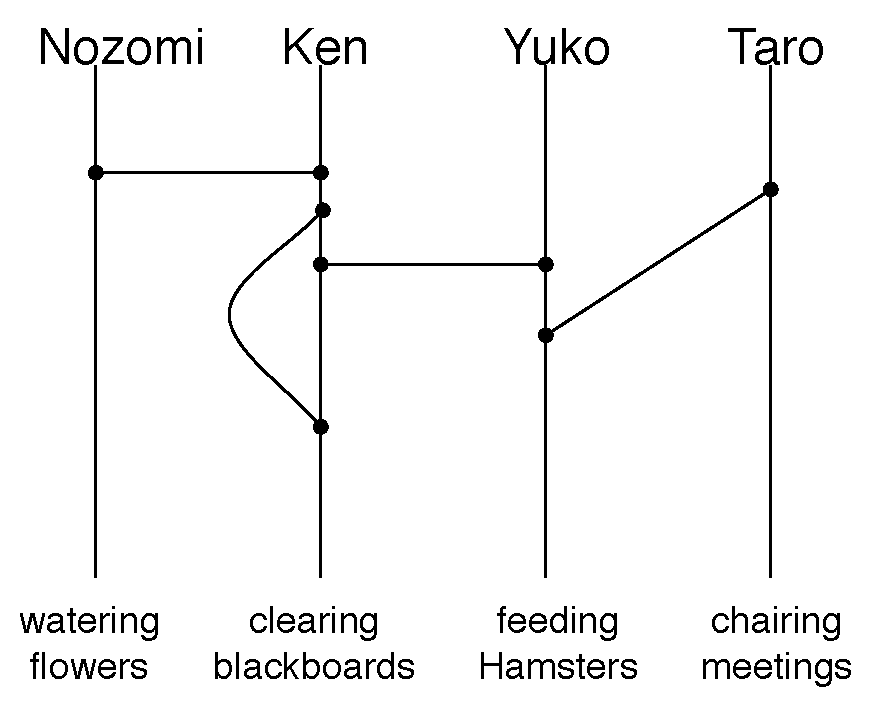
\includegraphics[scale=0.6]{amida.eps}
  \caption[An example of Amida lotteries.]{An example of Amida
  lotteries.  Nozomi clears blackboards; Ken waters flowers; Yuko chairs
  meetings; and Taro feeds Hamsters.}
  \label{amida-lottery}
 \end{figure}


\section{To the Next Chapters}

Each chapter can be read independently.
Chapter~\ref{ch:exchange} treats a synchronous hyper-lambda calculus and
Chapter~\ref{ch:lambda} deals with an asynchronous one.
The operational semantics is simpler in the synchronous case while
the type system is more exotic in the synchronous case.
The asynchronous one is apt for shared--memory implementation.
Chapter~\ref{ch:pole} treats another asynchronous hyper-lambda calculus
based on monoidal t-norm logic.  In this chapter, we analyse the
\textit{prelinearity
axiom}\index{axiom!prelinearity}\index{prelinearity}
$(\phi\limp\psi)\oplus(\psi\limp\phi)$ using the
parametricity argument.
Chapter~\ref{ch:haskell} implements a hyper-lambda calculus similar to
that in Chapter~\ref{ch:lambda} using Haskell.

\chapter{Inuitionistic Epistemic Logic}


We apply formal constructive reasoning to
 asyncyhronous communication.
After defining a general-purpose logic called
intuitionistic epistemic logic (\iec\,in
 short), 
we solve a~motivating example problem,
 characterising waitfree communication logically in response to the
 abstract simplicial topological characterisation of
 waitfree computation given by Herlihy, Shavit, Saks and Zaharoglou 
in the celebrated G\"odel Prize winning papers.

 Intuitionistic logic is originally a formalisation of a single mathematician whose
 knowledge
 increases over time.  The logic \iec\, formalises multiple agents who communicate
 asynchronously and whose knowledge increases over time.  
The logic \iec\, has a simple language: 
 it has epistemic modality but no temporal modality
 so that it is simpler than many previous logics for communication.
 We do not need temporal modality because 
we regard time as 
the partial order in the semantics of intuitionistic epistemic logic.
 Before defining the deduction system, we first extend the informal intuitionistic
 reading of logical connectives.
 Precisely, 
 we extend Brouwer--Heyting--Kolmogorov interpretation of logical connectives
 by adding one clause reagarding the additional epistemic modality~$K_a$.
 After stating the informal meaning for the modality,
 we define a deduction system and a Kripke semantics meeting this intuition.
 Soundness, strong completeness, finite
 model property, disjunction property and decidability are
 shown. 
We also investigate the relationship between \iec\,and classilcal modal logic with multple
 S4 modalities.

On top of the logic \iec, we give an axiom type that characterises
 sequential consistency for shared memory.
 The advantage of intuitionistic logic over classical logic is shown
 in an example where a set of axioms characterises 
 sequential consistency on shared memory.
 The axioms for sequential consistency are
 meaningless in classical logic while
 meaningful in intuitionistic logic.
 The axioms are similar to 
 the axiom type for prelinerilty.
 This similarity reflects the analogy 
 between sequential consistency for shared memory scheduling 
 and linearity for Kripke frames: both require antisymmetry on schedules or models.

Finally, under sequential consistency, we give soundness and completeness between
 a set of logical formulas called waitfree assertions and a set of models called 
schedule models.
 It has been found that it is undecidable whether a task is waitfreely solvable or not.
 We show that when we only view the communication requirements of tasks,
 it is decidable whether the communication is waitfreely attainable or not.


In the Master's thesis, we show that
formal constructive reasoning is
applicable to asynchronous communication.
We define a new logical deduction system called intuitionistic epistemic logic.
Although there are infinitely many possible deduction systems,
we propose this system because 
we are surprised to see that such a simple and useful logic has never been
proposed, or if ever, has not gained popularity.

There are at least two different ways of reasoning about knowledge.
In one view of knowledge using Kripke semantics,
which classical epistemic logic employs,
knowledge is defined as proposition valid in all possible worlds
that is possible to an agent.
On the other hand, knowledge can be seen as something agents can send and receive.
We unify these two notions of knowledge into the semantics of the logic we present.
We define the semantics formally in the style of Kripke semantics.
At the same time, 
an extension to BHK-interpretation reveals that asynchronous
communication is implicit in the formal definition.

\subsection{The Reason for Another Logic}

\paragraph{Motivation: reasoning about concurrent systems}
We give a formal deduction system for reasoning about
asynchronous communication.
The motivation for doing it is
the fact that creating a concurrently
working system with asynchronous communication 
and especially testing and debugging it is
notoriously difficult 
because of nondeterministic scheduling.
When the cost of testing and debugging is high,
it is reasonable to
spend more cost on ensuring correctness of the system
at earlier stages like designing phase or implementation phase, not testing and debugging.
In order to ensure correctness at an earlier stage,
it is crucially important to reason about the system correctly because
at such an early stage, knowledge about the system can only be obtained by reasoning,
not by testing.

\paragraph{Method: giving a formal deduction system}
A formal deduction system mathematically defines
available form of reasoning.
In order to define reasoning mathematically,
a formal deduction system uses languages defined mathematically.
The main advantage of the reasoning on a formal deduction system over
reasoning in a natural language
is the former is independent of most implicit assumptions
on which the latter is dependent so that
the validity of the former formal reasoning can be checked more rigorously
 than the latter informal reasoning.

We seek to have a formal
deduction system as simple and learnable as possible to reason about asynchronous
communication.
We choose to give an epistemic logic, i.e., a logic with an operator expressing an agent's
knowledge because mentioning agents' knowledge appeals to
human intuition.
For example, as Halpern and Zuck~\cite{halpern1992little}
 point out, Bochmann and Gecsei's paper~\cite{bochmann} written in 1977 already uses
 the notion of knowledge when reasoning about protocols:
\begin{quotation}
\noindent
 Verification \ldots will correspond
\ldots to finding out whether and in
which circumstances the sender \ldots
 can ``know'' that all data \ldots have been delivered correctly%
\footnote{The dots \ldots and a period by the author.}.
\end{quotation}

\paragraph{Previous work presumes a global clock unnecessarily}
Existing formal epistemic logic for reasoning about communication implicitly or
explicitly assume a global clock. Even if they are capable of reasoning about
asynchronous communication, they first consider the synchronous case and then define the
asynchrony in terms of ignorance of the global situation.
This way, asynchronous communication can be dealt with successfully as done in Halpern's
famous work~\cite{halpern1985formal,fagin2003reasoning}
However, the procedure of
considering the global clock and then forgetting it
makes formal reasoning unnecessarily complicated:
we propose a formal deduction system whose semantics does not contain the notion of
a global clock anywhere.

\subsection{Intuitionistic Epistemic Logic}

The main contribution of this thesis is giving definition of
intuitionistic epistemic logic (\iec\, for short) and investigating it.

\paragraph{Abstraction of Herlihy and Shavit's topological model}
In order
to reason about general asynchronous communication,
we abstracted some important features from the mathematical model for wait-free
computation proposed by Herlihy and Shavit~\cite{herlihy1999topological}.
The obtained model is abstract enough so that it can be described as a~Kripke model of
intuitionistic propositional logic equipped with additional functions on possible worlds.


\paragraph{Original intuitionistic meaning of knowledge}
 Agents in asynchronous systems can
 obtain knowledge about other agents only by receiving some constructions from them,
 not by waiting for a fixed length of time.
 This specific style of knowledge, where
 obtaining knowledge requires obtaining physical constructions,
 is the same as the style of knowledge of intuitionistic, constructive reasoners.
 That is the reason why we deliberately choose intuitionistic not classical meanings for
 the basic logical connectives, especially $\supset$ and $\vee$, although classical logic
 is more popularly used among computer scientists and mathematicians.
 The abstract Kripke model for asynchronous communication
 can be seen as a description of agents passing around constructions that ensure
 propositions.

 We extend the language of intuitionistic propositional logic with a unary operator $K_a$,
 whose meaning can be expressed as:
 a proof of $K_a\varphi$ is a construction that witnesses agent~$a$'s
 acknowledgement of a proof of $\varphi$ and also contains the acknowledged
 proof.  This formulation of knowledge is original.
 This meaning is different from that of classical epistemic logic where
 the meaning of $K_a$ can be expressed as:
 $K_a\varphi$ is valid if and only if $\varphi$ is valid in all possible worlds
 that agent~$a$ thinks possible.

 One advantage of our meaning of $K_a$ over that of classical meaning is that
 it can express communication without the help of another modality.
 Namely, in our meaning,
 a proof of $K_bK_a P$ is a construction that is passed from agent $a$ to agent
 $b$.
 On the other hand, in classical meaning, the same formula expresses nothing about
 communication:
 $K_b K_a P$ is valid when $P$ is valid in all possible worlds that agent~$b$ in any
 possible world that agent~$a$ thinks possible thinks possible.

Intuitionistic logic can be seen as a logic describing an agent whose knowledge increases over
time.
The logic \iec\,  can be seen as a logic describing multiple agents
that asynchronously communicate with each other and increase their knowledge.
Although \iec\, deals with communication, the logic has only epistemic modalities so that it
has simpler syntax than many other logics for communication.

\paragraph{The problem with classical logic}
Classical logic asserts the Law of Excluded Middle, which states
either a proposition or the negation of it is always valid.
The Law of Excluded Middle asserts that either 
a message has reached the intended receiver or it has not reached the intended receiver.
We point out that this reasoning assumes the existence of a current state of the world.
The notion of the current state implicitly assumes global clock within the use of the
adjective ``current''.
 
In classical epistemic logic, the description of knowledge relies on the notion of possible
worlds.
An agent can distinguish some pairs of possible worlds while
he or she cannot distinguish the other pairs of possible worlds.
When the actual state is one of the possible worlds,
agent $a$ knows something when it is valid in all possible worlds
indistinguishable from the actual state.
In this description of knowledge,
all possible states are considered to exist at the same time.
Knowledge change can only be modelled via a sequence of such models.
The sequence forms a global clock, which is unnecessary to describe asynchronous
communication.

For example, in dynamic epistemic logic~\cite{ditmarsch2007dynamic,van2003concurrent},
communication is instantaneous and forms common knowledge.
A message changes the model globally.
Although no clock appears syntactically,
the instantaneous change of models implicitly assumes
every agent shares the same uniform progress of time and
all events are lined up in a total order.
Dynamic epistemic logic might successfully describe human intuition on communication,
which is unfortunately incorrect for reasoning about asynchronous communication.
In fact, as Halpern~\cite{halpern1990knowledge} pointed out,
it is asynchronously impossible to form a new common knowledge.

Aside from dynamic epistemic logic, 
some logics~\cite{sato13study}
have numbering in syntax or in semantics that represents a global clock.
Although it is possible to understand asynchronous communication using a hypothetical
global clock and then forgetting it as in~\cite{halpern1990knowledge}
a model without a global clock would be simpler and more preferable according to
Occam's razor.

\paragraph{Reducing the number of design choices by identifying intuitionistic relation
    with temporal relation}
There were other choices: there have been proposed a huge number
 of epistemic logics for communication
\cite{halpern1990knowledge,van2009information,liau2003belief,%
plaza2007logics,%
balbiani2008knowable,%
 peleg1987communication,%
bieber1990logic,baltag2007epistemic,jia2004modal,costa2005formalizing}
and a huge
number of intuitionistic modal logics
\cite{hiroakira-some, 1029823, 1986,
alechina-categorical,
peleg1987communication}.
In both cases, when considered under Kripke semantics,
the huge variety of logics comes
 from the diversity of relationships
between two binary relations on the state space.
In intuitionistic modal logic, the two relations are:
(a) which state is prior to which state with regard to
Kripke monotonicity and (b) the modality in which state refers to which state.
In logics for communication, the two relationships are:
(a') which state is temporarily prior to which state and
(b') from which state to which state a communication occurs.

The semantics of \iec\, uses a
binary relation on the states and
\textit{functions} on the states instead of
additional binary relations.
For an agent to know something about another agent, it is necessary to
receive something from the other agent.
When an agent receives something from another agent,
the receiver can identify the sender.  We formalised this identification as a function on
the states.
This choice dramatically limits the
room for design choice.
Also, we identify relations
(a) with (a') and (b) with (b') in order to make the language of \iec\,
simpler.

\paragraph{Formalising available reasoning}
We give a deduction system and show
soundness (Theorem~\ref{soundness}), disjunction property (Theorem~\ref{disjunction-property}),
strong completeness
(Theorem~\ref{strong-completeness}), finite model property
 (Theorem~\ref{thm:fmp}) and decidability (Theorem~\ref{decidability}).

\subsection{Application to Wait-free Communication}

Since the semantics for \iec\, is inspired by the topological characterisation of wait-free
computation given by Herlihy and Shavit~\cite{herlihy1999topological},
we applied the logic \iec\, to wait-free computation in order to see
what change is caused by the abstraction of simplicial complexes to Kripke models.

\paragraph{Sequential consistency}
The topological characterisation by Herlihy and Shavit~\cite{herlihy1999topological}
implicitly assumes sequential consistency~\cite{lamport1979make} of shared memory.  
This motivated us to characterise sequential consistency with the axiom type
$(K_\memory \varphi\supset K_\memory \psi)\vee (K_\memory
       \psi\supset K_\memory \varphi)$
in the logic \iec\, for asynchronous computation.
Technically, we defined a class of models called sequential models
and proved soundness
(Lemma~\ref{sc-sound}) and completeness
 (Theorem~\ref{sc-comp}) of the axiom type with respect to the sequential models.

\paragraph{Wait-free communication}
A waitfree protocol over shared memory~\cite{herlihy1991wait}
 assigns a program to each process so that no process waits for another process.
Some tasks can be solved by a~well-chosen waitfree protocol while the others cannot.

For example, 
 it is waitfreely impossible for both of two processes to attain the input value of the other
 process.
 On the other hand, it is waitfreely possible for
 either one of two processes to attain the input value of the other process.
 A waitfree protocol that solves this task is:
\begin{itemize}
 \item process $a$ tells the memory $\memory$ that $\varphi$ holds, and then $\memory$ replies back to $a$,
 \item process $b$ tells the memory $\memory$ that $\psi$    holds, and then $\memory$ replies back to $b$.
\end{itemize}
After this protocol finishes,
  either $\varphi$ has been communicated from~$a$ to~$b$ 
or $\psi$ has
been communicated from~$b$ to~$a$.

In the
 logic \iec, this fact is represented by a judgement $K_aK_\memory{}K_a\varphi,
K_bK_\memory{}K_b\psi\vdashsc K_aK_b\psi\vee K_bK_a\varphi$,
which is deducible in \iec\, with
sequential consistency axioms~(Figure~\ref{hoge}).

Herlihy and Shavit~\cite{herlihy1999topological} characterised waitfree computation using
simplicial topology.
Using their characterisation,
Gafni and Koutsoupias~\cite{gafni1999three}
 showed that it is undecidable whether a task is waitfreely solvable
 or not.
When tasks are restricted to communication defined by 
a class of logical formulas that we call waitfree assertions,
we can characterise waitfreely available communication logically (Theorem~\ref{sc-comp})
and 
it is decidable whether a task is waitfreely solvable or not (Theorem~\ref{wf-dec}).

\subsection{Preliminaries and Notations}

We assume inductive definitions using BNF and coinductive definition.
$\powerset X$ denotes the powerset of $X$.
For a symbol or a sequence of symbols $p$, 
$p^+$ denotes repetition of $p$ more than zero times and
$p^*$ denotes repetition of $p$ more than or equal to zero times.

\section{Intuitionistic Epistemic Logic}
\label{iec}

In this section, we give a logic called intuitionistic epistemic logic.
The logic has epistemic modality $K_a$ in addition to ordinary logical connectives
$(\wedge, \vee, \supset, \bot)$ of propositional logic.
We explain the meaning of the new modality $K_a$ informally, by extending 
the Brouwer--Heyting--Kolmogorov interpretation (BHK-interpretation) of logical
connectives, which dates back to 1930's
 (Heyting~\cite{heyting1930formalen, heyting1931intuitionistische}
 are cited by Troelstra et al.~\cite{troelstra1988constructivism}).

\subsection{Formulas}

We fix a countably infinite set of propositional symbols
$PVar$ and a finite set of agents $A$.
Let $P, Q, \ldots$ run over the propositional symbols.

\begin{definition}
\label{formula}
 We define a \textit{formula} $\varphi$ by the BNF:
\[
 \varphi ::= \bot\mid P\mid
 (K_a\varphi)\mid(\varphi\vee\varphi)\mid(\varphi\wedge\varphi)\mid
 (\varphi\supset\varphi)
\]
where $a\in A$ stands for an agent.
\end{definition}
We sometimes omit the parenthesis when no confusion occurs. We use $=$ for syntactic
equality of formulas. 
The notation $(\neg \varphi)$ stands for $(\varphi\supset \bot)$.
For a sequence of formula $\Gamma = (\varphi_i)$, the notation $K_a \Gamma$ stands for
the sequence $(K_a \varphi_i)$.

\subsection{Informal Explanation by BHK-Interpretation}
\label{bhk}

Intuitionistic meanings for logical connectives
can be presented as 
following sentences called BHK-interpretation\footnote{
Taken from Troelstra and van Dalen's textbook~\cite[Ch.~1]{troelstra1988constructivism}:
author made notational modification of logical formulas and omission of
quantifiers $\forall$ and $\exists$.
}:
\begin{quotation}
\noindent
\begin{description}
 \item[(H1)] A proof of $\varphi\wedge \psi$ is given by presenting a proof of $\varphi$
	    and a proof of $\psi$.
 \item[(H2)] A proof of $\varphi\vee\psi$ is given by presenting either a proof of
	    $\varphi$ or a proof of $\psi$ (plus the stipulation that we want to regard
	    the proof presented as evidence for $\varphi\vee\psi$\footnote{In fact, the
	    author considers this as not enough. A proof $\varphi\vee\varphi$ must contain
	    the choice of the left $\varphi$ or the right $\varphi$.}).
 \item[(H3)] A proof of $\varphi\supset\psi$ is a construction which permits us to
	    transform any proof of $\varphi$ into a proof of $\psi$.
 \item[(H4)] Absurdity $\bot$ (contradiction) has no proof; a proof of $\neg \varphi$ is a
	    construction which transforms any hypothetical proof of $\varphi$ into a proof
	    of a contradiction.
\end{description}
\end{quotation}
In this paper, we consider extending BHK-interpretation with another stipulation for
epistemic modality:
\begin{description}
 \item[(HK)] A proof of $K_a\varphi$ is a construction that witnesses agent~$a$'s
	    acknowledgement of a proof of $\varphi$ and also contains the acknowledged
	    proof.
\end{description}
We choose to regard knowledge as acknowledgement of proofs so that the modality $K_a$ informally
describes knowledge of agent~$a$.
The formalisation of knowledge is different from that in classical epistemic logic, where
knowledge is described as a limitation on the ability to distinguish possible worlds.

\subsection{Deduction System}

\noindent The unary operators connect more strongly than the binary operators.
We sometimes omit the parentheses when no confusion occurs. We use $=$ for syntactic
equality of formulas. 
The notation $(\neg \varphi)$ stands for $(\varphi\supset \bot)$.
For a sequence of formulas $\Gamma = (\varphi_i)_{i\in I}$ or a set of formulas~$\Gamma$,
the notation $K_a \Gamma$ stands for the sequence $(K_a \varphi_i)_{i\in I}$ or the set
$\{K_a\varphi\mid \varphi\in \Gamma\}$ respectively.

\begin{figure*}
\begin{center}
\AxiomC{}
\LeftLabel{(ax)}
\UnaryInfC{$\varphi \vdash \varphi$}
\DisplayProof
\hfill
\AxiomC{$\Gamma\vdash\varphi$}
\LeftLabel{(w)}
\UnaryInfC{$\psi,\,\Gamma\vdash\varphi$}
\DisplayProof
 \hfill
\AxiomC{$ \varphi,\,\varphi,\,\Gamma\vdash\varphi'$}
\LeftLabel{(c)}
\UnaryInfC{$\varphi,\,\Gamma\vdash\varphi'$}
\DisplayProof
\hfill
\AxiomC{$\Gamma, \varphi,\psi,\, \Gamma'\vdash\varphi'$}
\LeftLabel{(e)}
\UnaryInfC{$\Gamma,\,\psi,\varphi,\,\Gamma'\vdash\varphi'$}
\DisplayProof
\vskip 5mm
\AxiomC{$\Gamma\vdash \varphi\wedge\psi$}
\LeftLabel{($\wedge$-E$_0$)}
\UnaryInfC{$\Gamma\vdash \varphi$}
\DisplayProof
\hfill
\AxiomC{$\Gamma\vdash\varphi$}
\AxiomC{$\Gamma'\vdash\psi$}
\LeftLabel{($\wedge$-I)}
\BinaryInfC{$\Gamma,\Gamma'\vdash \varphi\wedge\psi$}
\DisplayProof
\hfill
\AxiomC{$\Gamma\vdash \varphi\wedge\psi$}
\LeftLabel{($\wedge$-E$_1$)}
\UnaryInfC{$\Gamma\vdash \psi$}
\DisplayProof
\vskip 5mm
\AxiomC{$\Gamma\vdash \varphi$}
\LeftLabel{($\vee$-I$_0$)}
\UnaryInfC{$\Gamma\vdash \varphi\vee\psi$}
\DisplayProof
\hfill
\AxiomC{$\Gamma\vdash \varphi$}
\LeftLabel{($\vee$-I$_1$)}
\UnaryInfC{$\Gamma\vdash \psi\vee\varphi$}
\DisplayProof
\vskip 5mm
\AxiomC{$\Gamma\vdash \psi_0\vee\psi_1$}
\AxiomC{$\Gamma,\,\psi_0\vdash \varphi$}
\AxiomC{$\Gamma,\,\psi_1\vdash \varphi$}
\LeftLabel{($\vee$-E)}
\TrinaryInfC{$\Gamma\vdash \varphi$}
\DisplayProof
\vskip 5mm
\AxiomC{$\varphi,\,\Gamma\vdash\psi$}
\LeftLabel{($\supset$-I)}
\UnaryInfC{$\Gamma\vdash \varphi\supset\psi$}
\DisplayProof
\hfill
\AxiomC{$\Gamma\vdash\psi_0\supset\psi_1$}
\AxiomC{$\Gamma\vdash \psi_0$}
\LeftLabel{($\supset$-E)}
\BinaryInfC{$\Gamma\vdash \psi_1$}
\DisplayProof
\hfill
\AxiomC{$\Gamma\vdash\bot$}
 \LeftLabel{($\bot$-E)}
 \UnaryInfC{$\Gamma\vdash\varphi$}
 \DisplayProof
\hfill
\AxiomC{$\Gamma\vdash K_a\varphi$}
\LeftLabel{(T)}
\UnaryInfC{$\Gamma\vdash \varphi$}
\DisplayProof
\vskip 5mm
\AxiomC{$\Gamma \vdash K_a\varphi$}
 \LeftLabel{(ispec)}
\UnaryInfC{$\Gamma\vdash K_a K_a \varphi$}
\DisplayProof
 \hfill
 \AxiomC{$\Gamma\vdash\varphi$}
\LeftLabel{(nec)}
\UnaryInfC{$K_a\Gamma\vdash K_a\varphi$}
\DisplayProof
\hfill
\AxiomC{$\Gamma\vdash K_a(\varphi\vee\psi)$}
\LeftLabel{($\vee K$)}
 \UnaryInfC{$\Gamma\vdash K_a \varphi\vee K_a\psi$}
\DisplayProof
\end{center}
\caption[Deduction rules of \iec.]
{Deduction rules of \iec.  (ax) stands for axiom, (w) for weakening, (c) for
 contraction, (e) for exchange, (ispec) for introspection and (nec) for necessitation.
 ($\diamondsuit$-I) denotes the introduction rule for connective~$\diamondsuit$.
 ($\diamondsuit$-E) denotes the elimination rule for connective~$\diamondsuit$.}
\label{fig}
\end{figure*}

We give a proof system of \iec\, in natural deduction.
Most of the rules are common with intuitionistic propositional logic while some rules are added
to define the meaning of the $K_a$ modality.
\begin{definition}
 We define the proof system of \iec\, by Figure~\ref{fig}.
 The system is presented in the form of usual schemata.
 A proof diagram is a finite tree of deduction rules with one bottom node with the
 following property: when a node has a judgement
 above the line, there is a node immediately above it and the above node
 has the same judgement below the line.
\end{definition}

\paragraph{Rationales for the rules on modalities}

While the rules (T), (ispec) and (nec) are admissible in classical epistemic logic,
we have an additional rule ($\vee K$) which needs explanation.
In this paragraph, we are going to give a rationale for the rule ($\vee K$) with the help
of BHK-interpretation given in Subsection~\ref{bhk}.
A proof for the premise of the rule ($\vee K$) is a construction that witnesses agent~$a$'s
acknowledgement of a proof of $\varphi\vee\psi$.
Since a proof of $\varphi\vee\psi$ is either a proof of $\varphi$ or a proof of $psi$,
agent~$a$'s acknowledge of a proof of $\varphi\vee\psi$ implies either agent~$a$'s
acknowledgement of a proof of $\varphi$ or agent~$a$'s acknowledgement of a proof of $\psi$.

Also, 
we are informally
assuming logical omniscience of the agents by rule (nec),
 that is, we assume agents have complete
command on intuitionistic epistemic logic so that they acknowledge every formulas
deducible from the set of formulas they acknowledge.
We do not try to convince that every conceivable agent has logical omniscience.
We only speculate that agents without logical omniscience are hard to represent in a
formal system.

\paragraph{Notational conventions}
For a~set of formula~$\Gamma$ and a~formula~$\varphi$, $\Gamma\vdash
\varphi$ denotes a~relation where
there is such a~finite sequence~$\Gamma_0$ that 
$\Gamma_0\vdash
\varphi$ is deducible and that $\Gamma_0$ contains only formulas in $\Gamma$.

\subsection{Semantics}
We define validity of a~formula on a~state in a~model.
A~model is a~Kripke model for propositional intuitionistic logic
equipped with an additional
mapping $f_a: W\rightarrow W$ for each agent $a\in A$ where $W$ is the
set of possible states.
Informally\footnote{This account is informal in that we do not attempt to
define the terms ``view'' and ``current state''.},
 the function $f_a$ represents the view of agent
$a$.
When the current state is $w\in W$\kern -2pt, agent $a$ sees that the current state is
$f_a(w)\in W$, in other words, agent $a$ knows everything valid in $f_a(w)$.
As a special consequence, agent $a$ knows that agent $b$ sees that the current state
is
$f_b(f_a(w))\in W$\kern -2pt.
This model is an abstraction of Herlihy and Shavit's model of waitfree
computation~\cite{herlihy1999topological}.
See Subsection~\ref{Shavit} for details.

\newcommand{\model}[1]{\tuple{W#1, \preceq#1, (f_a#1)_{a\in A}, \rho#1}}
\begin{definition}
\label{model}
 A \textit{model} $\tuple{W,\preceq, (f_a)_{a\in A}, \rho}$ is a tuple with following properties:
\begin{enumerate}
 \item $\tuple{W,\preceq}$ is a partial order,
 \item $f_a\colon W\rightarrow W$ is a~function satisfying
\begin{enumerate}
 \item (descendance) $f_a(w) \preceq w$,
 \item (idempotency) $f_a(f_a(w)) = f_a(w)$, and
 \item (monotonicity) $w\preceq v$ implies $f_a(w)\preceq f_a(v)$
\end{enumerate}
       for all $v,w\in W$,
 \item $\rho\colon PVar\rightarrow \powerset W$ is a function such that each $\rho(P)$ is
       upward-closed with respect to $\preceq$, i.e., $w'\succeq w\in\rho(P)$ implies
       $w'\in\rho(P)$.
\end{enumerate}
\end{definition}
\noindent With the informal account in mind, the conditions on $f_a$ have rationales:
descendance condition says an agent~$a$ recognises only truth, 
idempotency says an agent $a$ recognises that 
       $a$ recognises something whenever the agent~$a$ recognises that thing,
and monotonicity says an agent~$a$ does not forget things recognised.
Differently from classical epistemic logic,
there is no distinction between global states and local states.

The valuation~$\rho$ for propositional variables in $PVar$ is extended into validity
relation~$\models$ for all formulas in $\fml$.
\begin{definition}
 We define the \textit{validity relation} $\models$ of a~model
 $\tuple{W,\preceq,(f_a)_{a\in A},\rho}$, a~state~$w\in W$ of the model and a
 formula~$\varphi$.
 Let us fix a model $M=\tuple{W,\preceq,(f_a)_{a\in A},\rho}$.
\newcommand{\m}{M}
 The definition of $M,w\models\varphi$ is inductive on the structure of $\varphi$.
\begin{description}
 \item[(Case $\varphi=\bot$)] $\m, w\models \bot$ never holds.
\item[(Case $\varphi= P$)] $\m, w\models P$ if and only if 
$w \in
 \rho(P)$.
 \item[(Case $\varphi = K_a \psi$)] 
	    $\m, w\models K_a \psi$ if and only if
	    $\m, f_a(w)\models \psi$.
\item[(Case $\varphi = \psi_0\wedge\psi_1$)]
 $\m, w\models \psi_0\wedge\psi_1$ if and only if both
 $\m, w\models \psi_0$ and $\m,w\models \psi_1$ hold.
\item[(Case $\varphi = \psi_0\vee\psi_1$)]
 $\m, w\models \psi_0\vee\psi_1$ if and only if either
 $\m, w\models \psi_0$ or $\m,w\models \psi_1$ holds.
\item[(Case $\varphi = \psi_0\supset \psi_1$)]
	   $\m, w\models \psi_0\supset\psi_1$ if and only if 
	   for any $w'\in W$ with $w'\succeq w$, the validity $M,w'\models \psi_0$ implies
	   the validity $M, w'\models
	   \psi_1$.
\end{description}
\end{definition}

Next, we show that the restriction on the valuation~$\rho$ is preserved by the extension
to validity~$\models$. Informally, this theorem presents the limitation of the logic \iec:
it can only deal with propositions whose validity is preserved by progress with respect to
the partial order $\preceq$ belonging to the model.
\begin{theorem}[Kripke monotonicity]
\label{kripke}
$M,w\models \varphi$ and $w\preceq v$ imply
$M,v\models \varphi$.
\end{theorem}
\begin{proof}
 By structural induction on $\varphi$.
 We fix a~model~$M$ and we abbreviate $M,w \models
 \varphi$ into $w\models \varphi$.
\begin{description}
 \item[(Case $\varphi = \bot$)]  The assumption $w\models \bot$ never holds.
 \item[(Case $\varphi = P$)] By the restriction on $\rho$ in Definition~\ref{model}.
 \item[(Case $\varphi = K_a \psi$)] 
	    By monotonicity of $f_a$ and induction hypothesis.
 \item[(Case $\varphi = \psi_0\wedge\psi_1$)] 
	    Assume $w\models \psi_0\wedge \psi_1$.
	    Both $w\models \psi_0$ and $w\models \psi_1$ hold. 
	    By induction hypothesis, $v\models\psi_0$ and
	    $v\models\psi_1$ hold.
	    Thus
	    $v\models \psi_0\wedge \psi_1$ holds.
 \item[(Case $\varphi = \psi_0\vee\psi_1$)] 
	    Similarly by induction hypothesis.
 \item[(Case $\varphi =\psi_0\supset\psi_1$)]
	    By definition of $\models$.
\end{description}
\end{proof}

\paragraph{Semantics of judgements}

We introduce some notations which look similar to the judgements appearing in the 
deduction
system.
Being aware of the different definitions of $\vdash$ and $\models$, we are going to
compare the two relations $\vdash$ and $\models$ in the next subsections.

\begin{notation}
For a~model~$M$ and a~state~$w$ of the model,
we write $M,w\models \Gamma$ when the validity
$M,w\models\varphi$ holds for any formula $\varphi$ in $\Gamma$.
\end{notation}

\begin{notation}
$\Gamma\models\varphi$ stands for the relation of formula
 sequences $\Gamma$ and a~formula
 $\varphi$ that holds if and only if for any model $M$ 
and $w\in M$, $M,w\models \Gamma$ implies
 $M,w\models \varphi$.
\end{notation}

\begin{definition}
$\Gamma\models\varphi$ stands for the relation of a set of a formulas
 $\Gamma$ and a formula~$\varphi$ where $M,w\models \Gamma$ implies
 $M,w\models \varphi$ for any model~$M$ 
and a~state~$w\in M$.
\end{definition}
For a~sequence of formulas $\Gamma$, we let $u(\Gamma)$ denote the set of formulas
appearing in $\Gamma$.  We abbreviate $u(\Gamma)\models\varphi$ into
$\Gamma\models\varphi$. We will sometimes write $\Gamma$ instead of $u(\Gamma)$ for the
sake of brevity.

\begin{definition}
 A set of formulas $\Gamma$ is consistent if and only if $\Gamma\not\models \bot$.
\end{definition}

\subsection{Soundness}

Soundness is the single most important feature of a formal deductive system because the
main reason for using a formal deductive system is it ensures correct reasoning.
We regard the defined semantics as a standard for correct reasoning and show that the
deduction systems of \iec\, meets that standard.
Soundness ensures a formula provable in \iec\, is valid in any state of any model.
At the same time, we show a stronger notion:
a formula provable under a set of assumptions is always valid whenever the assumptions are
valid.

\begin{theorem}[Soundness]
\label{soundness}
$\Gamma\vdash\varphi$ implies $\Gamma\models\varphi$.
\end{theorem}
\begin{proof}
We prove soundness with induction on the definition of $\vdash$. 
 We fix a~model~$M$ and we abbreviate $M,w \models
 \varphi$ into $w\models \varphi$.
\begin{description}
 \item[(ax)(w)(c)(e)] Trivial.
 \item[($\supset$-I)] Assume $\Gamma,\varphi\models\psi$.
	    Assume $w\models \Gamma$. Also assume that there is such a~state $w'$
	    in $M$ that $w'\succeq w$ and
	    $w'\models\varphi$ hold. 
	    By Lemma~\ref{kripke}, $ w'\models\Gamma$ holds.
	    Since $\Gamma,\varphi\models\psi$, the relation $\Gamma, w'\models
	    \psi$ holds.
 \item[($\supset$-E)]
	    Assume $\Gamma\models\varphi\supset\psi$ and $\Gamma\models\varphi$.
	    By the second assumption, $w\models \varphi$ holds.
	    The first assumption says $w\models\varphi\supset\psi$.
	    Since $w\succeq w$, the relation $w\models\psi$ holds.
 \item[($\wedge$-I)($\vee$-I$_0$)($\vee$-I$_1$)($\vee$-E)($\wedge$-E$_0$)($\wedge$-E$_1$)]
	    Trivial.
 \item[(T)] Assume $w\models \Gamma$. By induction hypothesis,
	    the validity $w\models K_a \varphi$ holds.
	    By definition of $\models$, 
	    $ f_a(w)\models\varphi$ holds.
	    Since $f_a(w)\preceq w$, Lemma \ref{kripke} says
	    $w\models \varphi$.
 \item[(inspec)]
	    Assume $w\models \Gamma$.
	    By induction hypothesis, the validity
	    $w\models\varphi$ holds. By definition of $\models$,
	    $f_a(w)\models\varphi$ holds.
	    Since $f_a$ is idempotent, 
	    $f_a(f_a(w))\models\varphi$.
	    Applying the definition of $\models$ again in the opposite direction,
	    we obtain
	    $w\models{K_a}\varphi$.
 \item[(nec)] 
	    Assume $\Gamma\models\varphi$ and
	    $ w\models{K_a}\Gamma$ hold.
	    Since $w\models\Gamma$, the first assumption says $w\models \varphi$.
	    By definition of $\models$, the relation
	    $w\models{K_a} \varphi$ holds.
 \item[($\vee{K_a}$)]
	    Assume $\Gamma\models {K_a}(\varphi\vee\psi)$.
	    For any state $w$ of any model $M$, assume
	    $w\models{K_a}(\varphi\vee\psi)$.
	    By the definition of $\models$,
	    $f_a(w)\models\varphi\vee\psi$.
	    Applying the definition of $\models$ again,
	    either $f_a(w)\models\varphi$ or $f_a(w)\models\psi$ holds.
	    This implies either $w\models{K_a}\varphi$ or $w\models{K_a}\psi$
	    holds.
	    We have $w\models{K_a}\varphi\vee{K_a}\psi$. 
\end{description}
\end{proof}


\subsection{Disjunction Property}

We modify Aczel's slash and prove disjunction property.
We referred Troelstra and van Dalen's textbook~\cite[3.5]{troelstra1988constructivism}
for the proof of disjunction property of intuitionistic propositional logic.

The main originality of this subsection is the following definition of the function $f_a$.
Informally, for a set $\Gamma$ of formulas,  $f_a(\Gamma)$ is agent~$a$'s view of the
set~$\Gamma$.
\begin{definition}
 \label{gafa}
 For an agent $a\in A$, we define 
 two functions $g_a, f_a\colon \powerset{\fml}\rightarrow \powerset{\fml}$ as
\begin{align*}
 g_a(\Gamma)&=\{\varphi\in\fml\mid (K_a)^+\varphi\in\Gamma\text{ and }\varphi\text{ does
 not begin with }K_a\},\\
 f_a({\Gamma}) &= g_a(\Gamma) \cup K_ag_a(\Gamma) \cup \{\varphi\in\fml\mid \Gamma\vdash\bot\}.
\end{align*}
 where $(K_a)^+$ denotes a finite repetition of at least one $(K_a)$.
\end{definition}

\subsubsection{Properties of the Auxiliary Functions}

Since the definition for the auxiliary function~$f_a$ is not very straightforward,
it is worthwhile checking some properties of it like monotonicity and idempotency.
Actually, in the next subsection, a variant of this function $f_a$ will be used for
constructing a model so that its monotonicity and idempotency are necessary.

\begin{proposition}
 \label{g_mono}
 $\Gamma\subseteq \Delta$ implies $g_a(\Gamma)\subseteq g_a(\Delta)$.
\end{proposition}
\begin{proof}
 By the form of definition of $g_a$ in Definition~\ref{gafa}.
\end{proof}

\begin{proposition}
 \label{cupg}
 $g_a(\Delta\cup \Gamma) = g_a(\Delta)\cup g_a(\Gamma)$.
\end{proposition}
\begin{proof}
 By the form of definition of $g_a$ in Definition~\ref{gafa}.
\end{proof}

\begin{proposition}
 \label{cupf}
 $f_a(\Delta\cup \Gamma)$ is equal to
 $f_a(\Delta)\cup f_a(\Gamma)$ provided $\Delta\cup\Gamma\not\vdash\bot$.
\end{proposition}
\begin{proof}
 \begin{align*}
  f_a(\Delta\cup\Gamma)& = g_a(\Delta\cup\Gamma)\cup K_ag_a(\Delta\cup\Gamma)
  &\text{(definition of $f_a$)}\\
  &= g_a(\Delta)\cup g_a(\Gamma)\cup K_ag_a(\Delta)\cup K_ag_a(\Gamma)
  &\text{(Proposition~\ref{cupg})}\\
  &= g_a(\Delta)\cup K_ag_a(\Delta)\cup g_a(\Gamma)\cup K_ag_a(\Gamma)
  &\text{(reordering)}\\
  &= f_a(\Delta)\cup f_a(\Gamma)
  &\text{(definition of $f_a$)}.
 \end{align*}
\end{proof}

\begin{proposition}
 \label{f_mono}
 $\Gamma\subseteq \Delta$ implies $f_a(\Gamma)\subseteq f_a(\Delta)$.
\end{proposition}
\begin{proof}
 If $\Delta\vdash\bot$, $f_a(\Gamma)\subseteq \fml = f_a(\Delta)$.
 Otherwise, 
 there exists a set $\Gamma'$ with $\Gamma\cup \Gamma' = \Delta$.
 Using Proposition~\ref{cupf} suffices.
\end{proof}

\begin{proposition}
 \label{wakame}
 For any $\varphi\in K_af_a(\Gamma)$, $\Gamma\vdash\varphi$ holds.
\end{proposition}
\begin{proof}
 $\varphi = K_a\psi$ where $\psi\in f_a(\Gamma) = g_a(\Gamma)\cup K_ag_a(\Gamma)\cup
 \{\varphi\in\fml\mid\Gamma\vdash\bot\}$.
 \begin{description}
  \item[ (Case $\psi\in g_a(\Gamma)$)]
	     By~definition of $g_a$, $(K_a)^+\psi\in \Gamma$.
	     By~rule~(T), $\Gamma\vdash K_a\psi$.
	     This is what we sought: $\Gamma\vdash\varphi$.
  \item[ (Case $\psi\in K_ag_a(\Gamma)$)]
	     $\psi = K_a\psi'$ where $\psi'\in g_a(\Gamma)$.
	     By the same argument, $\Gamma\vdash K_a\psi'$.
	     By~rule~(inspec), $\Gamma\vdash K_aK_a\psi'$.
	     This is what we sought: $\Gamma\vdash\varphi$.
  \item[ (Case $\Gamma\vdash\bot$)]
	     By rule ($\bot$-E), $\Gamma\vdash\varphi$ holds.
 \end{description}
\end{proof}

\begin{proposition}
 \label{kombu}
 For any $\varphi\in f_a(\Gamma)$, $\Gamma\vdash\varphi$ holds.
\end{proposition}
\begin{proof}
 $K_a\varphi\in K_af_a(\Gamma)$. By~Proposition~\ref{wakame},
 $\Gamma\vdash K_a\varphi$ holds.
 By~rule~(T), deducibility $\Gamma\vdash\varphi$ holds.
\end{proof}

\begin{proposition}
 \label{f_double}
 $f_a(f_a(\Gamma)) = f_a(\Gamma)$.
\end{proposition}
\begin{proof}
 If $\Gamma\not\vdash\bot$, by Proposition~\ref{kombu}, $f_a(\Gamma)\not\vdash\bot$ also holds.
 \begin{align*}
  f_a(f_a(\Gamma))
  &= f_a(g_a(\Gamma)\cup K_ag_a(\Gamma))
  &\text{(definition of $f_a$)}
\\
  &= f_a(g_a(\Gamma))\cup f_a(K_ag_a(\Gamma))
  &\text{(Proposition~\ref{cupf})}
\\
  &= \emptyset \cup f_a(\Gamma)
  &\text{(definitions of $f_a$ and $g_a$)}
\\
  &= f_a(\Gamma).
 \end{align*}
 Otherwise, if $\Gamma\vdash\bot$,
 $f_a(\Gamma) = \fml = f_a(f_a(\Gamma))$.
\end{proof}

\subsubsection{The Slash Relation}

\newcommand{\aslash}[0]{\mathbin{\mid}}
We use $f_a$ defined above to extend Aczel's slash relation to the language of \iec.
We add a clause for $K_a$ modalities where we use the function $f_a$.
\begin{definition}
 We define the slash relation $\aslash$ as follows:
 \begin{align*}
  \Gamma\aslash\bot& \Longleftrightarrow \Gamma\vdash\bot, \\
  \Gamma\aslash{}P& \Longleftrightarrow \Gamma\vdash P, \\
  \Gamma\aslash K_a\varphi &\Longleftrightarrow f_a(\Gamma)\aslash\varphi
  \\
  \Gamma\aslash \varphi \wedge \psi & \Longleftrightarrow \Gamma\aslash\varphi\text{
  and }\Gamma\aslash\psi,\\
  \Gamma\aslash \varphi\vee\psi &\Longleftrightarrow \Gamma\aslash\varphi\text{ or
  }\Gamma\aslash\psi,\\
  \Gamma\aslash \varphi\supset\psi &\Longleftrightarrow \Delta\aslash\varphi
  \text{ implies
  }\Delta\aslash\psi \text{ for any } \Delta\supseteq\Gamma
  \text{ and also }\Gamma\vdash{}\varphi\supset\psi.
 \end{align*}
\end{definition}

\begin{lemma}
\label{ssound}
 $\Gamma\aslash\varphi\Rightarrow \Gamma\vdash\varphi.$
\end{lemma}
\begin{proof}
 By induction on $\varphi$.
 \begin{description}
  \item[ (Case $\varphi = \bot$)(Case $\varphi = P$)]
	     By definition of $\aslash$.
  \item[ (Case $\varphi = K_a\psi$)]
	     The assumption $\Gamma\aslash K_a\psi$ is equivalent to 
	     $f_a(\Gamma)\aslash \psi$.
	     By induction hypothesis,
	     $f_a(\Gamma)\vdash \psi$.
	     By rule (nec), 
	     $K_af_a(\Gamma)\vdash  K_a\psi$.
	     By Proposition~\ref{wakame},
	     the deducibility $\Gamma\vdash K_a\psi$ holds.
  \item[ (Case $\varphi = \psi_0 \wedge \psi_1$)]
	     $\Gamma\aslash\psi_0\wedge \psi_1$.
	     By definition of $\aslash$,
	     Both $\Gamma\aslash\psi_0$ and $\Gamma\aslash\psi_1$ hold.
	     By induction hypothesis,
	     both $\Gamma\vdash K_x\psi_0$ and
	     $\Gamma\vdash K_x\psi_1$ hold.
	     By logic, $\Gamma\vdash K_x(\psi_0\wedge\psi_1)$ holds.
  \item[ (Case $\varphi = \psi_0\vee\psi_1$)]
	     Similar to the case above.
  \item[ (Case $\varphi = \psi_0\supset \psi_1$)]
	     By definition of $\aslash$.
 \end{description}
\end{proof}

\begin{lemma}
 \label{aslash-mono}
$\Gamma\aslash\varphi$ and $\Gamma\subseteq \Delta$ imply $\Delta\aslash\varphi$.
\end{lemma}
\begin{proof}
 By induction on $\varphi$.
 \begin{description}
  \item[ (Case $\varphi=\bot$) (Case $\varphi =P$) (Case $\varphi =\psi_0\supset \psi_1$)]
	     By definition of the slash relation $\aslash$.
  \item[ (Case $\varphi =\psi_0\wedge\psi_1$) (Case $\varphi =\psi_0\vee\psi_1$)]
	     Directly from induction hypotheses.
  \item[ (Case $\varphi = K_a\psi$)]
	     By Proposition~\ref{f_mono},
	     $f_a(\Gamma)\subseteq f_a(\Delta)$ holds.
	     By induction hypothesis, $f_a(\Gamma)\aslash \psi$ implies
	     $f_a(\Delta)\aslash\psi$, which is equivalent to $\Delta\aslash\varphi$ holds.
 \end{description}
\end{proof}

\begin{lemma}
 \label{ugougo}
 For any set $\Gamma$ of formulas with $\Gamma\aslash\psi$ for all $\psi\in\Gamma$,
 $\varphi\in g_a(\Gamma)$ implies $f_a(\Gamma)\aslash\varphi$.
\end{lemma}
\begin{proof}
 By definition of $g_a$, $(K_a)^{(n)}\varphi\in \Gamma$ for some $n\ge 1$, where
 $(K_a)^{(n)}$ denotes an~$n$-time repetition of $K_a$'s.
 By assumption, $\Gamma\aslash (K_a)^{(n)}\varphi$.
 By definition of $\aslash$, $f_a^{(n)}(\Gamma)\aslash\varphi$.
 Since $f_a$ is idempotent~(Proposition~\ref{f_double}), $f_a(\Gamma)\aslash \varphi$.
\end{proof}

This definition of hereditary $f$-closed formulas is original.
\begin{definition}
 A hereditary $f$-closed set $\Gamma$ is coinductively defined as:
 $\Gamma$ is a hereditary $f$-closed set if and only
 if $f_a(\Gamma)$ is hereditary $f$-closed and $f_a(\Gamma)\subseteq \Gamma$ for all $a\in
 A$.
\end{definition}
Equivalently, we can define the negation inductively as:
\begin{itemize}
 \item if $f_a(\Gamma) \not\subseteq \Gamma$, $\Gamma$ is not a hereditary $f$-closed set.
 \item if $\Gamma$ is not a hereditary $f$-closed set, $f_a(\Gamma)$ is not a hereditary
       $f$-closed set.
\end{itemize}
For example, the set $\Gamma = \{K_b K_a K_a P\}$ is not hereditary $f$-closed
because $f_b(\Gamma)$ is not hereditary $f$-closed.
$f_b(\Gamma)$ is not hereditary $f$-closed
 because $K_a P \in f_a(f_b(\Gamma))$ while $K_a P\notin f_b(\Gamma)$.

 Since $f_a(\emptyset) = \emptyset$  for any $a\in A$,
 $\emptyset$ is a hereditary $f$-closed set.

\begin{lemma}
 \label{absurd}
 For any hereditary $f$-closed set 
 $\Gamma$ and a formula $\varphi$,
 $\Gamma\vdash\bot$ implies $\Gamma\aslash\varphi$.
\end{lemma}
\begin{proof}
 By induction on $\varphi$.
 \begin{description}
  \item[ (Case $\varphi =\bot$) (Case $\varphi =P$)]
	     $\Gamma\vdash\varphi$ implies $\Gamma\aslash\varphi$ because $\varphi$ is
	     atomic.
  \item[ (Case $\varphi = K_a\psi$)]
	     Since $f_a(\Gamma)$ is also hereditary $f$-closed and $\bot\inf_a(\Gamma)$,
	     by induction hypothesis, $f_a(\Gamma)\aslash\psi$.
	     This is equivalent to $\Gamma\aslash K_a\psi$.
  \item[ (Case $\varphi = \psi_0\wedge\psi_1$) (Case $\varphi = \psi_0\vee\psi_1$)]
	     Directly from induction hypothesis.
  \item[ (Case $\varphi = \psi_0\supset\psi_1$)]
	     By rule ($\bot$-E), $\Gamma\vdash\psi_0\supset\psi_1$.
	     For all $\Delta\supset\Gamma$, by induction hypothesis,
	     $\Delta\aslash\psi_1$ holds.
	     These two facts show $\Delta\aslash\psi_0\supset\psi_1$.
 \end{description}
\end{proof}

\begin{lemma}
 For any hereditary $f$-closed set $\Gamma$ of formulas,
 if $\Gamma\aslash \psi$ for all $\psi\in\Gamma$,
 $f_a(\Gamma)\aslash \varphi$ for all $\varphi \in f_a(\Gamma)$.
\end{lemma}
\begin{proof}
  By induction on the structure of $\varphi$. However, most cases are uniformly treated in
 the last clause.
 \begin{description}
  \item[ (Case $\varphi = K_x\psi$)]
	     Assume $K_x\psi\in f_a(\Gamma) = g_a(\Gamma)\cup K_ag_a(\Gamma)\cup
	     \{\theta\in\fml\mid\Gamma\vdash\bot\}$.
	     \begin{description}
	      \item[ (Case $K_x\psi\in g_a(\Gamma)$)]
			 By~Lemma~\ref{ugougo}, $f_a(\Gamma)\aslash K_x\psi$.
	      \item[ (Case $K_x\psi\in K_ag_a(\Gamma)$)]
			 Note $x = a$.
			 By~Lemma~\ref{ugougo},
			 $f_a(\Gamma)\aslash\psi$ holds.
			 Since $f_a$ is idempotent,
			 $f_a(f_a(\Gamma))\aslash\psi$ holds.
			 By definition of $\aslash$,
			 $f_a(\Gamma)\aslash K_a\psi$.
	      \item[ (Case $\Gamma\vdash\bot$)]
			 $f_a(\Gamma)\vdash\bot$ also holds.
			 By Lemma~\ref{absurd}, $f_a(\Gamma)\aslash\varphi$ holds.
	     \end{description}
  \item[ (Other cases)] 
	     Assume $\varphi\in f_a(\Gamma) = g_a(\Gamma)\cup K_ag_a(\Gamma)\cup
	     \{\theta\in\fml\mid\Gamma\vdash\bot\}$.
	     If $\Gamma\vdash\bot$, by Lemma~\ref{absurd} and definition of $f_a$,
	     $f_a(\Gamma)\aslash\varphi$.
	     Otherwise, since the formula $\varphi$ does not begin with $K_a$,
	     $\varphi\in g_a(\Gamma)$.
	     By~Lemma~\ref{ugougo}, $f_a(\Gamma)\aslash\varphi$.
 \end{description}
\end{proof}


\begin{lemma}
 \label{T}
 $\Gamma\aslash K_a\varphi\Rightarrow \Gamma\aslash\varphi$ if $\Gamma$ is $f_a$-closed.
\end{lemma}
\begin{proof}
 Immediate from Lemma~\ref{aslash-mono}.
\end{proof}

\begin{lemma}
 \label{slash-deduction}
 $\Gamma\aslash\psi$ and $\Gamma\cup\{\psi\}\aslash
 \varphi$ imply $\Gamma\aslash\varphi$.
\end{lemma}
\begin{proof}
 By induction on $\varphi$.
 \begin{description}
  \item[ (Case $\varphi = \bot$) (Case $\varphi = P$)]
	     Since $\Gamma\aslash\psi$, by Lemma~\ref{ssound},
	     the deducibility $\Gamma\vdash\psi$ holds.
	     Likewise since $\Gamma\cup \{\psi\}\aslash\varphi$, the deducibility $\Gamma\cup
	     \{\psi\}\vdash \varphi$ holds.
	     These combined imply $\Gamma\vdash\varphi$.
	     By definition of the slash relation $\aslash$, the relation
	     $\Gamma\aslash\varphi$ holds because $\varphi$ is
	     atomic. 
  \item[ (Case $\varphi = \psi_0\vee\psi_1$) (Case $\varphi =\psi_0\wedge\psi_1$)]
	     Directly from induction hypotheses.
  \item[ (Case $\varphi = K_a\theta$)]
	     Since $\Gamma\cup\{\psi\}\aslash K_a\theta$, by definition of the slash
	     relation $\aslash$,
	     $f_a(\Gamma\cup\{\psi\})\aslash \theta$ holds.
	     If $\Gamma\cup\{\psi\}\vdash\bot$, by the assumption,
	     $\Gamma\vdash\bot$. Thus, by Lemma~\ref{absurd}, $\Gamma\vdash\varphi$ holds.
	     Otherwise, since $f_a(\Gamma\cup\{\psi\}) = f_a(\Gamma)\cup f_a(\{\psi\})$,
	     we have $f_a(\Gamma)\cup f_a(\{\psi\})\aslash \theta$.
	     If $\psi = K_a\psi'$,
	     $\Gamma\aslash\psi$ is equivalent to $f_a(\Gamma)\aslash \psi'$.
	     By induction hypothesis, $f_a(\Gamma)\aslash\theta$.
	     This is equivalent to $f_a(\Gamma)\aslash K_a\theta$.
	     This is what we sought: $f_a(\Gamma)\aslash\varphi$.
	     Otherwise, if $\psi$ does not begin with $K_a$,
	     $f_a(\{\psi\}) = \emptyset$.
	     Thus, $f_a(\Gamma)\aslash\theta$.
	     This means $\Gamma \aslash K_a\theta$.
  \item[ (Case $\varphi = \psi_0\supset\psi_1$)]
	     Since $\Gamma\cup\{\psi\}\aslash \psi_0\supset\psi_1$,
	     by Lemma~\ref{ssound},
	     $\Gamma\cup\{\psi\}\vdash\psi_0\supset \psi_1$ holds.
	     In addition to this,
	     $\Delta\cup\{\psi\}\aslash \psi_0$ implies
	     $\Delta\cup\{\psi\}\aslash \psi_1$ for any $\Delta\supseteq \Gamma$.
	     We claim that $\Delta\aslash \psi_0$ implies $\Delta\aslash \psi_1$ for any
	     $\Delta\supseteq \Gamma$.
	     To show that, we assume $\Delta\aslash\psi_0$.
	     By Lemma~\ref{aslash-mono},
	     $\Delta\cup\{\psi\}\aslash \psi_0$ holds.
	     By assumption, $\Delta\cup\{\psi\}\aslash\psi_1$ holds.
	     By induction hypothesis, $\Delta\aslash\psi_1$ holds.
	     We have shown that 
	     $\Delta\aslash \psi_0$ implies $\Delta\aslash \psi_1$.
	     In addition to this, by $\Gamma\vdash\psi$ and
	     $\Gamma\cup\{\psi\}\vdash\psi_0\supset\psi_1$, the deducibility
	     $\Gamma\vdash\psi_0\supset \psi_1$ holds.
	     The slash relation $\Gamma\aslash\psi_0\supset \psi_1$ has been proved.
 \end{description}
\end{proof}

\begin{lemma}
 \label{equiv}
 If $\Gamma$ and $\Delta$ are provably equivalent and satisfy
 $f_a(\Gamma) = f_a(\Delta)$ for all $a\in A$,
 $\Gamma\aslash\varphi$ is equivalent to $\Delta\aslash\varphi$.
\end{lemma}
\begin{proof}
 By the form of the definition of the slash relation $\aslash$.
\end{proof}

\subsubsection{Disjunction Property}

The standard proof for disjunction property is extended to the logic \iec.

\begin{theorem}
\label{slashcomp}
For any hereditary $f$-closed set $\Gamma$ of formulas, 
 if $\Gamma\aslash\varphi$ holds for any $\varphi \in \Gamma$\kern -1pt,
 $\Gamma\vdash\varphi$ implies $\Gamma\aslash\varphi$.
\end{theorem}
\begin{proof}
 By induction on definition of $\Gamma\vdash\varphi$.
 \begin{description}
  \item[ (ax) (w) (c) (e)] Trivial.
  \item[ ($\wedge$-E$_i$) ($\wedge$-I) ($\vee$-I$_i$)] By definition of the slash relation
	     $\aslash$.\vskip 3mm
  \item[ ($\vee$-E)]
\AxiomC{$\Gamma\vdash \psi_0\vee\psi_1$}
\AxiomC{$\Gamma,\,\psi_0\vdash \varphi$}
\AxiomC{$\Gamma,\,\psi_1\vdash \varphi$}
\TrinaryInfC{$\Gamma\vdash \varphi$}
\DisplayProof\vskip 4mm
	     By an induction hypothesis, $\Gamma\aslash \psi_0\vee\psi_1$ holds.
	     By definition of the slash relation,
	     either $\Gamma\aslash\psi_0$ or $\Gamma\aslash\psi_1$ holds.
	     \begin{description}
	      \item[ (Case $\Gamma\aslash\psi_0$)]
			 By another induction hypothesis,
			 $\Gamma\cup \{\psi_0\}\aslash \varphi$ holds.
			 By~Lemma~\ref{slash-deduction},
			 $\Gamma\aslash\varphi$ holds.
	      \item[ (Case $\Gamma\aslash\psi_1$)]
			 Similar.
	     \end{description}\vskip 3mm
  \item[ ($\supset$-I)]
	     \AxiomC{$\varphi,\,\Gamma\vdash\psi$}
\UnaryInfC{$\Gamma\vdash \varphi\supset\psi$}
\DisplayProof
\vskip 4mm
	     By induction hypothesis, $\varphi\cup \Gamma\aslash\psi$ holds.
	     Thus for any $\Delta\supseteq \Gamma$, $\varphi\cup \Delta\aslash\psi$ holds.
	     $\Delta\aslash\varphi$ implies $\Delta\aslash\psi$
	     by~Lemma~\ref{slash-deduction}.
	     This fact and the deducibility $\Gamma\vdash\varphi\supset\psi$ imply
	     $\Gamma\aslash\varphi\supset\psi$.\vskip 3mm
  \item[ ($\supset$-E)]
\AxiomC{$\Gamma\vdash\psi_0\supset\psi_1$}
\AxiomC{$\Gamma\vdash \psi_0$}
\BinaryInfC{$\Gamma\vdash \psi_1$}
\DisplayProof
\vskip 4mm
	     By induction hypothesis,
	     $\Gamma\aslash\psi_0\supset\psi_1$ holds.
	     By definition of the slash relation, $\Gamma\aslash\psi_0$ implies
	     $\Gamma\aslash\psi_1$.
	     Actually, $\Gamma\aslash\psi_0$ holds by an induction hypothesis.
	     Thus, $\Gamma\aslash\psi_1$ holds.
  \item[ ($\bot$-E)] By Lemma~\ref{absurd}.\vskip 3mm
  \item[ (T)] \AxiomC{}\UnaryInfC{$K_a\varphi\vdash\varphi$}\DisplayProof\\
	     Assume $K_a\varphi\in\Gamma$\kern -1pt.
	     By assumption of the theorem, $\Gamma\aslash K_a\varphi$.
	     Since $\Gamma$ is $f_a$-closed,
	     by Lemma~\ref{T}, $\Gamma\aslash \varphi$.\vskip 3mm
  \item[ (nec)] \AxiomC{$\Delta\vdash\varphi$}\UnaryInfC{$K_a\Delta\vdash K_a\varphi$}
	     \DisplayProof \vskip 4mm
	     We can assume $K_a\Delta\subseteq \Gamma$ and that $\varphi\in\Gamma$
	     implies $\Gamma\aslash \varphi$.
	     Also, by induction hypothesis, any $\Gamma'$ with $\Delta\subseteq \Gamma'$
	     and $\psi\in\Gamma'\Rightarrow \Gamma'\aslash\psi$,
	     $\Gamma'\aslash\varphi$ holds.
	     Since $\Delta$ is a finite sequence,
	     there exists a natural number $n$ with
	     $\Delta\subseteq f_a(\Gamma)\cup K_af_a(\Gamma)\cup\cdots\cup
	     (K_a)^{(n)}f_a(\Gamma)$.
	     By induction hypothesis,
	     $f_a(\Gamma)\cup K_af_a(\Gamma)\cup\cdots\cup
	     (K_a)^{(n)}f_a(\Gamma)\aslash \varphi$ holds.
	     By Lemma~\ref{equiv}, this is equivalent to $f_a(\Gamma)\aslash \varphi$.
	     By definition of $\aslash$, $\Gamma\aslash K_a\varphi$ holds.
  \item[ ($\vee K$)]
	     \AxiomC{}
	     \UnaryInfC{$K_a(\varphi\vee\psi)\vdash (K_a \varphi)\vee K_a\psi$}
	     \DisplayProof \\
	     The proof can be pictorially shown as follows:
	     \begin{align*}
	      K_a(\varphi\vee\psi)& \Longrightarrow \Gamma\aslash K_a(\varphi\vee\psi)
	      &\text{(assumption)}
	      \\ & \Longleftrightarrow
	      f_a(\Gamma)\aslash \varphi\vee\psi
	      & \text{(definition of the slash relation~$\aslash$)}
	      \\ & \Longleftrightarrow
	      f_a(\Gamma)\aslash\varphi \text{ or } f_a(\Gamma)\aslash\psi
	      & \text{(definition of the slash relation~$\aslash$)}
	      \\ & \Longleftrightarrow
	      \Gamma\aslash K_a\varphi \text{ or } \Gamma\aslash K_a\psi
	      & \text{(definition of the slash relation~$\aslash$)}
	      \\ & \Longleftrightarrow
	      \Gamma\aslash K_a\varphi\vee K_a\psi
	      & \text{(definition of the slash relation~$\aslash$)}.
	     \end{align*}
 \end{description}
\end{proof}

Using the apparatus prepared above, we can finally show disjunction property,
which is the standard for constructive logic.
\begin{theorem}[Disjunction property]
 \label{disjunction-property}
 If $\vdash\varphi\vee\psi$ holds, either $\vdash\varphi$ or $\vdash\psi$ holds.
\end{theorem}
\begin{proof}
 Taking $\Gamma = \emptyset$ in Theorem~\ref{slashcomp},
 $\vdash\varphi\vee\psi$ implies $\emptyset\aslash\varphi$ or $\emptyset\aslash\psi$.
 By Lemma~\ref{ssound}, either $\vdash\varphi$ or $\vdash\psi$ holds.
\end{proof}

\subsection{Strong Completeness and Finite Model Property}

In this subsection, we show strong completeness and finite model property.
Since both proofs contain model construction,
most parts of both proofs can be written in the same lemmas.
 This utilisation of similarity of finite model property and strong completeness 
is originally the idea of
Sato~\cite{sato13study}.

\begin{definition}
We modify $f_a$ introduced in the last subsection (Definition~\ref{gafa}) and define $f'_a$ as:
 \[
  f'_a(\Gamma) = g_a(\Gamma) \cup K_ag_a(\Gamma).
 \]
\end{definition}

For some pages, we argue about a
set of formula $\Omega$. Later, when we show
strong completeness, we take $\Omega$ to be the whole set of well formed formulas.  Also,
when we show finite model property, we take $\Omega$ to be the set of the subformulas of a
certain formula.  This model construction is inspired by
Sato's paper~\cite{sato13study}
 and Troelstra and van Dalen's textbook~\cite{troelstra1988constructivism}.
 However, the notion of $f'$-subformula-closed sets is new and original.

\begin{definition}
\label{saturated-set}
 For a set of formulas $\Omega$, 
 a set of formulas $\Gamma\subseteq\Omega$ is \textit{$\Omega$-saturated} if and only if
\begin{enumerate}
 \item $\Gamma$ is $\Omega$-deductively closed, i.e., $\Gamma\vdash\varphi\in
       \Omega\Rightarrow
       \varphi\in\Gamma$,
 \item $\Gamma\vdash\varphi\vee\psi \Rightarrow \Gamma\vdash\varphi$ or $\Gamma\vdash\psi$
       if $\varphi,\psi\in\Omega$,
 \item $\Gamma\not\vdash\bot$.
\end{enumerate}
\end{definition}

\begin{definition}
 A hereditary $f'$-subformula-closed set $\Gamma$ is coinductively defined as:
 $\Gamma$ is a hereditary $f'$-subformula-closed set if and only
 if $f'_a(\Gamma)$ is hereditary $f'$-closed, $\Gamma$ is closed for taking subformulas and 
$f'_a(\Gamma)\subseteq \Gamma$.
\end{definition}

\begin{definition}
 We define $s_a(\varphi)$ inductively on $\varphi$:
\[
 s_a(\varphi) = \begin{cases}
		 s_a(K_a\psi) & \text{(if $\varphi = K_aK_a\psi$)},\\
		 \varphi & \text{(otherwise)}.
		\end{cases}
\]
\end{definition}
\noindent The function $s_a$ replaces every $K_aK_a$ with $K_a$ repeatedly so that there are no
$K_aK_a$ occurrences left.

\begin{lemma}
\label{fpreserve}
 For a hereditary $f'$-subformula-closed set $\Omega$, 
 if $\Gamma$ is an $\Omega$-saturated set,
 $f_a(\Gamma)$ is an $f'_a(\Omega)$-saturated set.
\end{lemma}
\begin{proof}
 We first make sure that $f_a(\Gamma)$ is a subset of $f'_a(\Omega)$.
 By definition of $f_a$, $f_a(\Gamma) = g_a(\Gamma)\cup
 K_ag_a(\Gamma)\cup\{\bot\in\fml\mid \Gamma\vdash\bot\}$.
 Since $\Gamma$ is an $\Omega$-saturated set, $\Gamma\not\vdash\bot$ so that
 $f_a(\Gamma) = g_a(\Gamma)\cup K_ag_a(\Gamma)$.
 On the other hand, $f'_a(\Omega) = g_a(\Omega)\cup K_ag_a(\Omega)$.
 Since $g_a(\Gamma)\subseteq g_a(\Omega)$
 by Proposition~\ref{g_mono}, $f_a(\Gamma)\subseteq f'_a(\Omega)$ holds.

 We check each condition of Definition~\ref{saturated-set} to make sure
 that $f_a(\Gamma)$ is
 actually an~$f'_a(\Omega)$-saturated set.
\begin{enumerate}
 \item Assume $f_a(\Gamma)\vdash\varphi$ and $\varphi\in f'_a(\Omega)$.
       $\varphi\in g_a(\Omega)\cup K_ag_a(\Omega)$ holds.
       \begin{description}
	\item[ (Case $\varphi\in g_a(\Omega)$)]
		   Note that $\varphi$ does not begin with $K_a$.
		   By definition of $g_a$,
		   $(K_a)^+\varphi\in\Omega$.
		   Since $\Omega$ is subformula-closed,
		   $K_a\varphi\in\Omega$ holds.
		   By $\Gamma\vdash K_a\varphi$, since $\Gamma$ is $\Omega$-saturated,
		   $K_a\varphi\in \Gamma$.
		   Thus, $\varphi\in f_a(\Gamma)$.
	\item[ (Case $\varphi\in K_ag_a(\Omega)$)]
		   $\varphi = K_a\varphi'$ and $\varphi'\in g_a(\Omega)$ hold.
		   Note that $\varphi'$ does not begin with $K_a$.
		   By definition of $g_a$,
		   $(K_a)^+\varphi'\in\Omega$.
		   This implies $K_a\varphi'\in\Omega$.
		   Since $\Gamma\vdash K_aK_a\varphi'$,
		   $\Gamma\vdash K_a\varphi'$ holds.
		   Thus, since $\Gamma$ is $\Omega$-saturated,
		   $K_a\varphi'\in \Gamma$ holds.
		   This means $\varphi = K_a\varphi' \in f_a(\Gamma)$.
       \end{description}
 \item Assume $f_a(\Gamma)\vdash\varphi\vee\psi$ and
       $\varphi,\psi\in f'_a(\Omega)$.
       By rule~(nec), $K_af_a(\Gamma)\vdash K_a(\varphi\vee\psi)$ holds.
       By~Proposition~\ref{wakame},
       the formulas in $K_af_a(\Gamma)$ are deducible from $\Gamma$.
       Thus, $\Gamma\vdash K_a(\varphi\vee\psi)$ holds.
       By rule ($\vee K$) and the fact that $\Gamma$ is saturated,
       either $K_as_a(\varphi)\in\Gamma$ or $K_as_a(\psi)\in\Gamma$ holds.
       We can assume $K_as_a(\varphi)\in\Gamma$ without loss of generality.
       This implies $f_a(\Gamma)\vdash\varphi$ and then
       $\varphi\in f_a(\Gamma)$.
 \item Seeking contradiction, assume $f_a(\Gamma)\vdash\bot$.
       Since $\Gamma\vdash K_a\bot$, the deducibility
       $\Gamma\vdash\bot$ holds, which contradicts the fact that
       $\Gamma$ is an $\Omega$-saturated set.
\end{enumerate}
\end{proof}

\newcommand{\natpls}{{\mathbb N}^{+}}

\begin{lemma}[Saturation lemma]
\label{lemma:saturation}
 For sets of formulas $\Gamma$ and $\Omega$ with $\Gamma\not\vdash\varphi$, 
 $\Gamma\subseteq \Omega$ and $\varphi \in \Omega$,
there exists an~$\Omega$-saturated
 set~$\Gamma^\omega$ with $\Gamma^\omega\not\vdash\varphi$
 and $\Gamma\subseteq \Gamma^\omega$.
\end{lemma}
\begin{proof}
 Since both $PVar$ and $A$ are countable, we can enumerate all formulas
 of $\Omega$ in a sequence
 $(\varphi_i)_{i\in\natpls}$.
 We define $\Gamma^i$ inductively:
\begin{description}
 \item[(Case $i = 0$)] $\Gamma^0 = \Gamma$,
 \item[(Case $i > 0$)] $\Gamma^i =
\begin{cases}
\{\varphi_{i}\}\cup \Gamma^{i-1} & \text{(if
 $\{\varphi_{i}\}\cup\Gamma^{i-1}\not\vdash\varphi$)}, \\
\Gamma^i = \Gamma^{i-1} \cup\{\varphi_{i}\supset\varphi\} &\text{(otherwise if
 $\varphi_i\supset \varphi\in \Omega)$},\\
 \Gamma^i = \Gamma^{i-1} &\text{(otherwise)}.
\end{cases}$
\end{description}
Using these $\Gamma^i$\kern -1pt, we define $\Gamma^\omega = \bigcup_{i\in\omega}
 \Gamma^i$\kern -1pt.
\noindent Since $\Gamma^0 = \Gamma$\kern -2pt, $\Gamma^\omega$ contains
 $\Gamma$\kern -2pt.

\noindent
\textbf{Claim:} 
 $\Gamma^\omega \not\vdash \varphi$.
Seeking contradiction, assume a deducibility $\Gamma^\omega\vdash\varphi$. 
Since only finite number of formulas in $\Gamma$ are used to prove $\varphi$,
there exists 
 a minimal~$i$ with
 $\Gamma^i\vdash\varphi$. Since $\Gamma\not\vdash\varphi$, $i$ is not 0.
 Since $\Gamma^i\neq \Gamma^{i-1}$, 
 either $\Gamma^i = \{\varphi_{i}\} \cup \Gamma^{i-1}$ 
or $\Gamma^i = \{\varphi_{i}\supset\varphi\}\cup \Gamma^{i-1}$ holds.
 The first case is explicitly forbidden.
 In the second case, $\Gamma^{i-1},\varphi_{i}\supset\varphi\vdash \varphi$ holds.
 That means $\Gamma^{i-1}\vdash (\varphi_{i}\supset\varphi)\supset \varphi$.
 Also, since we could not take the first case, $\Gamma^{i-1},\varphi_{i}\vdash \varphi$
 holds. That means $\Gamma^{i-1}\vdash \varphi_{i}\supset\varphi$.
 By these combined, $\Gamma^{i-1}\vdash\varphi$ holds, which contradicts to the minimality of
 $i$. The~claim is now proved.
\end{proof}

\noindent \textbf{Claim:}
$\Gamma^\omega$ is an~$\Omega$-saturated set.
\begin{proof}[Proof of Claim]
We check each condition listed in
 Definition~\ref{saturated-set}:
\begin{enumerate}
 \item  Assume $\Gamma^\omega \vdash \psi\in\Omega$. There is $i\in\natpls$ with $\varphi_i = \psi$.
 We know that $\Gamma^{i-1}\cup\{\varphi_i\}\not\vdash\varphi$. It means
 $\psi\in\Gamma^\omega$.
 \item Assume $\psi_0\vee\psi_1\in\Gamma^\omega$ and $\psi_0,\psi_1\in\Omega$.
       Seeking contradiction, assume $\psi_0\notin\Gamma^\omega$ and
       $\psi_1\notin\Gamma^\omega$.
       By~construction, both $\Gamma^\omega\vdash \psi_0\supset \varphi$ and 
       $\Gamma^\omega\vdash\psi_1\supset \varphi$ hold.
       Since $\Gamma^\omega$ is deductively closed, by ($\vee$-E) rule, we have $\Gamma^\omega\vdash\varphi$,
       which contradicts to the previous fact.
 \item Since $\Gamma^\omega\not\vdash\varphi$, by rule~($\bot$-E), $\Gamma^\omega\not\vdash\bot$.
\end{enumerate}

\noindent Since $\Gamma^0 = \Gamma$\kern -2pt, $\Gamma^\omega$ contains $\Gamma$\kern -2pt. 
The lemma is now proved.
\end{proof}
 

\newcommand{\canon}[1]{#1^{\mbox{c}}}
\begin{definition}[Canonical model candidate]
\label{cancan}
 For a sset of formulas $\Omega$,
 we define $\canon M(\Omega)$ as a tuple $\model{^{\mbox{c}}}$ where:
\begin{itemize}
 \item $\canon W$ is the set of pairs of the form $(\Omega', \Gamma)$ where
       $\Gamma$ is an $\Omega'$-saturated set and
       $\Omega'$ is a hereditary $f'$-subformula-closed subset of $\Omega$.
 \item $(\Omega', \Gamma)\canon\preceq(\Omega'',\Delta)$ if and only if
       $\Omega'\subseteq \Omega''$ and $\Gamma\subseteq\Delta$,
 \item $\canon f_a((\Omega',\Gamma)) = (f'_a(\Omega), f_a(\Gamma))$
 \item $\canon \rho(P) = \{(\Omega',\Gamma)\in \canon W\mid P\in\Gamma\}$.
\end{itemize}
\end{definition}

\begin{lemma}[Canonical model]
The tuple $\canon M$ is a model.
\end{lemma}
\begin{proof}
First of all, $\canon f_a$ is actually a function $\canon
 W\rightarrow \canon W$ by Lemma~\ref{fpreserve}.
We check each condition in Definition~\ref{model} to
 make sure the tuple is actually a model:
 \begin{enumerate}
  \item $\canon\preceq$ is a partial order because set theoretic inclusion $\subseteq$ is a
	partial order.
  \item 
\begin{enumerate}
 \item $\canon f_a((\Omega', \Gamma)) = (f'_a(\Omega'), f_a(\Gamma))$.
       Since $\Omega'$ is hereditary $f'$-subset-closed,
       $f'_a(\Omega')\subseteq \Omega'$ holds.
       Now, showing $\Gamma\subseteq f_a(\Gamma)$ is enough.
       Take an arbitrary $\varphi\in f_a(\Gamma)$.
       Since $\Gamma\not\vdash\bot$,
       either $\varphi\in g_a(\Gamma)$ or $\varphi\in K_ag_a(\Gamma)$ holds.
       In either case, $(K_a)^*\varphi \in \Gamma$ holds.
       That means $\Gamma\vdash\varphi$.
       Since $\varphi\in\Omega'$, $\varphi \in \Gamma$ holds.
       Thus we have shown $\Gamma\subseteq f_a(\Gamma)$.
       This completes the proof of 
       $\canon f_a((\Omega', \Gamma)) \canon\preceq (\Omega', \Gamma)$.
 \item By Lemma~\ref{f_double},
       $f_a(f_a(\Gamma)) = f_a(\Gamma)$ holds.
       Similar argument gives $f'_a(f'_a(\Omega')) = f'_a(\Omega')$.
       These combined imply that $\canon f_a$ is idempotent.
 \item Both $f_a$ and $f'_a$ are monotonic with respect to set theoretic inclusion.
       This implies that $\canon f_a$ is monotonic with respect to $\canon \preceq$.
\end{enumerate}
  \item Immediate.
 \end{enumerate}
\end{proof}


\section{Axiom Type for Sequential Consistency}
\label{sc}

A schedule determines temporal partial order of events such as
message sending and receiving.
A correct program must behave correctly under every schedule.
Shared memory consistency is a restriction on schedules.
When a stronger memory consistency is posed, it is easier for programs to behave
correctly.  This is analogous to the fact
that when a stronger condition
is posed upon models, more formulas become valid.

In this subsection, we characterise sequential consistency with a set of axioms.
Sequential consistency defined by Lamport~\cite{lamport1979make} is essentially a condition requiring the states of memory lined up
in a total order.
We define a deduction system $\vdash_{SC}$ by adding an axiom type to \iec\, and
characterise sequential consistency.

Henceforth, we assume $A = \{\memory\}\cup P\quad (\memory\notin P)$, where $P$ is the
set of processes and $\memory$ represents the shared memory.

\subsection{Definitions}

Sequential consistency requires
the memory states to line up in a total order.
A straightforward way to model sequential consistency might be
choosing the set of memory states in the model
and then asserting the memory states are lined up in a total order.
Actually, we can identify a memory state as a state~$w$ with
$f_\memory(w) = w$ because this equation asserts that
the memory's state seen from the state~$w$ is the state~$w$ itself.
This straightforward modelling of sequential consistency turns out to be
in appropriate logically because there is no formula which holds exactly
in the models defined in that naive way.
Even when there are memory states $v$ and $w$ without
temporal relation between them,
if the whole model is consists of a part containing $v$ and another disjoint,
unrelated part
containing $w$,
no formula on no state can recognise the break of sequential consistency.
Considering this pitfall, we can model sequential consistency as a class of models defined below.
\begin{definition}
 A sequential model is a model where for any states $w, w'$ and $x$, 
$x\preceq w$, $x\preceq w'$, $f_\memory(w) = w$ and $f_\memory(w') = w'$ imply
 $w\preceq w'$ or $w'\preceq w$.
\end{definition}

\begin{definition}
We let $SC$ be the set of formula of the form
$(K_\memory \varphi\supset K_\memory \psi)\vee (K_\memory
       \psi\supset K_\memory \varphi)$.

We add a rule (SC) to the previous calculus $\vdash$:
\AxiomC{}
\LeftLabel{(SC)}
\UnaryInfC{$\vdash \varphi$}
\DisplayProof ($\varphi \in SC$)

We define $\Gamma\vdash_{SC}\varphi$ in the same way as $\Gamma\vdash\varphi$. 
\end{definition}
\noindent Note that all axioms in the set $SC$ are classical tautologies so that adding these axioms
to classical logic is meaningless.
This is the merit of using intuitionistic logic rather than classical logic.

\subsection{Soundness}
\begin{lemma}
 \label{sc-sound}
 $\vdash_{SC} \varphi \Rightarrow M\models\varphi$ for any sequential model~$M$.
\end{lemma}
\begin{proof}
 We extend the induction of Lemma~\ref{soundness} with a clause for the rule~(SC).
\begin{description}
 \item[(SC)] Seeking contradiction, assume $M, w\not\models (K_\memory \varphi\supset
	    K_\memory \psi)\vee (K_\memory \psi\supset K_\memory \varphi)$.
	    The definition for $\models$ says that there exist states $w_0, w_1\succeq w$
	    with $M, w_0\models K_\memory\varphi$,\quad $M, w_1\models K_\memory\psi$,\quad
	    $M, w_1\not\models K_\memory\psi$ and $M, w_0\not\models K_\memory\varphi$.
	    These and Kripke monotonicity (Lemma~\ref{kripke}) contradicts to the
	    assumption that $M$ is a sequential model.
\end{description}
Other cases are the same as Lemma~\ref{soundness}.
\end{proof}
\subsection{Strong Completeness}
\begin{definition}
 A set of formulas $\Gamma$ is \textit{SC-saturated} if and only if all of these
 conditions are satisfied:
\begin{enumerate}
 \item $\Gamma$ is SC-deductively closed, i.e., $\Gamma\vdashsc\varphi\Rightarrow \varphi\in\Gamma$,
 \item $\varphi\vee\psi\in\Gamma \Rightarrow \varphi\in\Gamma$ or $\psi\in\Gamma$,
 \item $\Gamma\not\vdashsc\bot$.
\end{enumerate}
\end{definition}

\begin{lemma}[Saturation lemma]
\label{sc-saturation}
 For a set of formulas $\Gamma$ with $\Gamma\not\vdashsc\varphi$, there exists a saturated
 set of formulas $\Gamma^\omega$ with $\Gamma^\omega\not\vdashsc\varphi$
 and $\Gamma\subset \Gamma^\omega$.
\end{lemma}
\noindent 
This lemma can be proved in the same way as Lemma~\ref{lemma:saturation} where each $\vdash$ is replaced by $\vdashsc$.

\renewcommand{\canon}[1]{#1^{\mbox{sc}}}
\begin{definition}[Canonical model candidate for sequential consistency]
 We define a tuple\\ $\canon M =\model{^{\mbox{\rm sc}}}$ in the same
 way as Definition~\ref{cancan} of $M^{\mbox{c}}$ except that 
 $\canon W$ is the set of SC-saturated sets of formulas.
\end{definition}

\begin{lemma}[Canonical model for sequential consistency]
The tuple $\canon M$ is a sequential model.
\end{lemma}
\begin{proof}
First, we can show, in the same way as before,
 that checking $\canon f_a$ is actually a function $\canon
 W\rightarrow \canon W$.
Also, checking each condition in Definition~\ref{model} is similar so that we see $\canon
 M$ is actually a model.
 Finally, to see that the model~$\canon M$ is sequential,
 let $\Gamma, \Delta$ and $\Theta$ be states of $\canon M$ and assume
 $\Theta\canon\preceq\Delta$, $\Theta \canon\preceq \Delta$, $\canon f_\memory(\Gamma) = \Gamma$ and
 $\canon f_\memory(\Delta) = \Delta$.
 We claim that either $\Delta\canon\preceq \Gamma$ or $\Gamma\canon\preceq \Delta$ holds.
 Seeking contradiction, deny the claim.
 Since the relation $\canon \preceq$ is actually the set theoretic inclusion, there exist
 formulas $\varphi$ and $\psi$ with $\varphi\in\Gamma$, $\varphi\notin\Delta$, $\psi\in
 \Delta$ and $\psi\notin \Gamma$.
 Since $\canon f_\memory(\Gamma) = \Gamma$,
 $K_a\psi\notin\Gamma$ and $K_a\varphi\in \Gamma$ hold.
 Similarly,
 $K_a\varphi\notin\Delta$ and $K_a\psi\in\Delta$ hold.
 Since $\Theta$ is SC-saturated, $(K_a\varphi\supset K_a\psi)\vee (K_a\varphi\supset
 K_a\psi)$ is in $\Theta$.
 The definition of saturation says either
 $K_a\varphi\supset K_a\psi\in \Theta$ or
 $K_a\psi\supset K_a\varphi\in\Theta$.
 Consequently, either $K_a\varphi\supset K_a\psi\in\Gamma$ or
 $K_a\psi\supset K_a\varphi\in\Delta$ holds.
 Each case leads to contradiction by deductive closedness of $\Gamma$ and
 $\Delta$.
\end{proof}

\begin{lemma}
\label{sc-exact}
 For an SC-saturated set of formulas $\Gamma$ and the canonical model for sequential
 consistency
$\canon M$,
 an equivalency $\varphi\in\Gamma\Longleftrightarrow \canon M, \Gamma\vdashsc\varphi$ holds.
\end{lemma}
\noindent This lemma can be proved in the same way as Lemma~\ref{exact}.

\begin{theorem}[Strong completeness for sequential consistency]
 \label{sc-comp}
$\Gamma\vdashsc\varphi$ holds if $M\models \Gamma$ implies $M\models\varphi$ for every
 sequential model~$M$.
\end{theorem}
\begin{proof}
 We show the contraposition: assuming $\Gamma\not\vdashsc\varphi$, we show
 that there exists a sequential model~$M$ that satisfies
 $M\models\Gamma$ but not $M\models\varphi$.
 By Lemma~\ref{sc-saturation},
 there is an~SC-saturated set of formula $\Gamma'$ with $\Gamma'\not\vdash\varphi$
 and $\Gamma'\supset\Gamma$.
 By Lemma~\ref{sc-exact},
 $\canon M, \Gamma'\models \Gamma$ but not $\canon M, \Gamma' \models \varphi$.
 These two facts deny $\Gamma\models\varphi$.
\end{proof}



\paragraph{Example Theorem}

In Introduction, we gave an example of deducible judgements of $\vdashsc$:\\
$K_aK_\memory{}K_a\varphi,
K_bK\memory{}K_b\psi\vdashsc K_aK_b\psi\vee K_bK_a\varphi$.
We give a proof for this judgement in Figure~\ref{hoge}.
\begin{sidewaysfigure}
{\tiny
\textsf{Part A}\\
 \AxiomC{}
 \LeftLabel{(ax)}
 \UnaryInfC{$K_bK_a(K_\memory K_a\varphi\supset K_\memory K_b\psi)\vdashsc
 K_bK_a(K_\memory K_a\varphi\supset K_\memory K_b\psi)$}
 \LeftLabel{(T)}
 \UnaryInfC{$K_b K_a(K_\memory K_a\varphi\supset K_\memory K_b\psi)\vdash K_a(K_\memory
 K_a \varphi \supset K_\memory K_b\psi)$}
 \AxiomC{}
 \LeftLabel{(ax)}
 \UnaryInfC{$K_\memory K_a\varphi\vdashsc K_\memory K_a\varphi$}
 \AxiomC{}
 \LeftLabel{(ax)}
 \UnaryInfC{$K_\memory K_a\varphi\supset K_\memory K_b\psi\vdashsc K_\memory
 K_a\varphi\supset K_\memory K_b \psi$}
 \LeftLabel{($\supset$-E)}
 \BinaryInfC{$K_\memory K_a\varphi, K_\memory K_a\varphi\supset K_\memory K_b\psi\vdashsc
 K_\memory K_b\psi$}
 \LeftLabel{(nec)}
 \UnaryInfC{$K_a K_\memory K_a\varphi, K_a(K_\memory K_a\varphi\supset K_\memory
 K_b\psi)\vdashsc K_a K_\memory K_b\psi$}
 \LeftLabel{($\supset$-I)}
 \UnaryInfC{$K_aK_\memory K_a\varphi\vdashsc K_a(K_\memory K_a\varphi\supset K_\memory
 K_b\psi) \supset K_a K_\memory K_b\psi$}
 \LeftLabel{($\supset$-E)}
 \BinaryInfC{$K_b K_a(K_\memory K_a\varphi\supset K_\memory K_b\psi), K_aK_\memory
 K_a\varphi\vdashsc K_a K_\memory K_b\psi$}
\LeftLabel{($\supset$-I)}
 \UnaryInfC{$K_b K_a(K_\memory K_a\varphi\supset K_\memory K_b\psi)\vdashsc 
 K_aK_\memory K_a\varphi\supset K_aK_\memory K_b\psi$}
\LeftLabel{($\vee$-I)}
 \UnaryInfC{$
K_b K_a(K_\memory K_a\varphi\supset K_\memory K_b\psi)\vdashsc 
(K_\memory K_a\varphi\supset K_\memory K_b\psi)
 \vee
 (K_\memory K_b\psi\supset K_\memory K_a\varphi)
$}
\DisplayProof
 \vskip 7mm

\textsf{Part B}\\
\vskip 2mm
\AxiomC{}
 \LeftLabel{(SC)}
 \UnaryInfC{$\vdashsc (K_\memory K_a\varphi\supset K_\memory K_b\psi)
 \vee
 (K_\memory K_b\psi\supset K_\memory K_a\varphi)$}
 \LeftLabel{(nec)}
 \UnaryInfC{$\vdashsc K_a\left((K_\memory K_a\varphi\supset K_\memory K_b\psi)
 \vee
 (K_\memory K_b\psi\supset K_\memory K_a\varphi)\right)$}
 \LeftLabel{($\vee K$)}
 \UnaryInfC{$\vdashsc K_a(K_\memory K_a\varphi\supset K_\memory K_b\psi)
 \vee
 K_a(K_\memory K_b\psi\supset K_\memory K_a\varphi)$}
 \LeftLabel{(nec)}
 \UnaryInfC{$\vdashsc K_b\left(K_a(K_\memory K_a\varphi\supset K_\memory K_b\psi)
 \vee
 K_a(K_\memory K_b\psi\supset K_\memory K_a\varphi)\right)$}
 \LeftLabel{($\vee K$)}
 \UnaryInfC{$\vdashsc K_b K_a(K_\memory K_a\varphi\supset K_\memory K_b\psi)
 \vee
 K_b K_a(K_\memory K_b\psi\supset K_\memory K_a\varphi)$}
\AxiomC{$\vdots$ \textsf{Part A}}
\AxiomC{$\vdots$ (same as left, swap $(a,b)$ and $(\varphi, \psi)$)}
 \LeftLabel{($\vee$E)}
 \TrinaryInfC{$\vdashsc
(K_aK_\memory K_a\varphi\supset K_aK_\memory K_b\psi)\vee
 (K_bK_\memory K_b\psi\supset K_bK_\memory K_a\varphi)
$}
 \DisplayProof
\vskip 7mm

\textsf{Part C}\\
\AxiomC{}
\LeftLabel{(ax)}
 \UnaryInfC{$K_aK_\memory K_a\varphi\vdashsc K_a K_\memory K_a\varphi$}
 \AxiomC{}
 \LeftLabel{(ax)}
 \UnaryInfC{$K_aK_\memory K_a\varphi\supset K_aK_\memory K_b\psi\vdashsc
K_aK_\memory K_a\varphi\supset K_aK_\memory K_b\psi$}
 \LeftLabel{($\supset$-E)}
 \BinaryInfC{$K_aK_\memory K_a\varphi\supset K_aK_\memory K_b\psi, K_aK_\memory
 K_a\varphi\vdashsc K_aK_\memory K_b\psi$}
 \AxiomC{}
 \LeftLabel{(ax)}
 \UnaryInfC{$K_\memory K_b\psi \vdashsc K_\memory K_b\psi$}
 \LeftLabel{(T)}
 \UnaryInfC{$K_\memory K_b\psi\vdashsc K_b\psi$}
 \LeftLabel{(nec)}
 \UnaryInfC{$K_a K_\memory K_b\psi\vdashsc K_a K_b\psi$}
 \LeftLabel{($\supset$-I)}
 \UnaryInfC{$\vdashsc K_a K_\memory K_b \psi\supset K_aK_b\psi$}
 \LeftLabel{($\supset$-E)}
 \BinaryInfC{$K_aK_\memory K_a\varphi\supset K_aK_\memory K_a\psi, K_aK_\memory
 K_a\varphi\vdashsc K_a K_b \psi$}
 \DisplayProof
 \vskip 7mm

\textsf{Main Part}\\
\AxiomC{$\vdots$ \textsf{Part B}}
\UnaryInfC{
$(K_aK_\memory K_a\varphi\supset K_aK_\memory K_b\psi)\vee
 (K_bK_\memory K_b\psi\supset K_bK_\memory K_a\varphi)
$
}
\AxiomC{$\vdots$ \textsf{Part C}}
 \UnaryInfC{$K_\memory{}K_a\varphi\supset K_\memory{}K_b\psi,\, K_aK_\memory{}K_a\varphi\vdashsc K_aK_b \psi$}
 \UnaryInfC{$K_\memory{}K_a\varphi\supset K_\memory{}K_b\psi,\, K_aK_\memory{}K_a\varphi\vdashsc K_a K_b \psi \vee K_b K_a \varphi$}
\AxiomC{$\vdots$ (same as left, swap $(a,b)$ and $(\varphi, \psi)$)}
\LeftLabel{$\vee$E}
\TrinaryInfC{$K_aK_\memory{}K_a\varphi, K_bK_\memory{}K_b\psi\vdashsc K_aK_b\psi\vee K_bK_a\varphi$}
\DisplayProof
}
\caption{A proof diagram for an example theorem in $\vdashsc$.}
\label{hoge}
\end{sidewaysfigure}


\section{Waitfree Computation}
\label{wf}

\subsection{Problem Domain}

A distributed program assigns a program to each process.
When we execute a distributed program,
processes obtain execution steps in the order determined by the scheduler.

A distributed program is waitfree when there exists such a fixed number $k$ that
under any schedule,
any process finishes before using $k$~steps.
The informal meaning of this condition is forbidding a process to wait for another
process.
Assuming a process~$p$ waits for another process~$q$ to do something,
under an unfriendly schedule, the condition for waitfreedom is broken.
Actually, under
a schedule giving the first $k$~steps exclusively to the process~$p$
the process~$q$ cannot do anything in those first $k$~steps while the process~$p$ waits
for the process~$q$ to do that something, thus breaking the wait-free condition.

Some tasks can be solved by a waitfree distributed program while others cannot.
In this section, we consider the problem of
distinguishing the waitfreely solvables task and the waitfreely unsolvable ones.
Although this problem is undecidable in general~\cite{gafni1999three},
we find an approximation problem that is decidable.

\subsection{Logical Representation of the Problem}

While sequential consistency is a restriction on schedules,
wait-freedom is a restriction on distributed programs.
The behaviour of distributed programs depend on the schedule%
\footnote{A motivation for introducing formal reasoning into the area of distributed
computation is in this fact, which makes testing harder.}.
The a correct distributed program can be described as
a distributed program which gives correct behaviour under any schedule.
This form of definition is similar to that of validity of logical a formula:
a valid logical formula is a formula which is satisfied by any model.
We consider the schedule v.s. distributed program relation is similar to
the formula v.s. model relation.
In Section~\ref{sc},
in this section, we express wait-freedom as a class of formulas.

A distributed program specifies
from which process, to which process, and in what order
signals are transmitted.
We consider the signal transimission in a logical formula.
In short, a modality over a modality like $K_a K_b P$ describes communication.
We regard processes as agents.
A propositional variable $I_a$ informally denotes the fact that the process~$a$ has
started.
A logical formula $K_b K_a I_a$ informally states
``the process~$a$ was aware of the fact that the process~$a$ had started,
and then told the fact to the process~$b$.''
Similarly, another formula $K_a K_b K_a I_a$ informally states
``the process~$a$ was aware of the fact that the process~$a$ had started,
and then told the fact to the process~$b$. The process~$b$ in turn told back to the
process~$p$ that the process~$q$ had received the fact from~$a$.''
The latter communication pattern can be obtained by programs described in the following lines:
\begin{enumerate}
 \item When process~$a$ starts, it sends a signal to the process~$b$, then waits for a
       reply from~$b$ and then terminates.
 \item When process~$b$ starts, it waits for a signal from the process~$a$,
       replies back to $a$, and then terminates.
\end{enumerate}
Unfortunately,
since this distributed program is not waitfree,
we cannot include the formula
$K_a K_b K_a I_a$
in the class of formulas representing waitfreedom.
We will define the class of formulas and call them waitfree protocol descriptions.

Actually, although a process running a waitfree program is forbidden to wait for another process,
it is allowed to wait for the shared memory\footnote{Otherwise, any communication
whatsoever would be impossible.}.
For example, after a process
 makes a read request to the shared memory,
 it is allowed to wait for a value from the shared memory.
 Also, after a process makes a write request to the shared memory,
 it is allowed to wait for an acknowledgement from the shared memory.
 That is why we introduced a special agent $\memory\in A$ representing the shared memory.
 We call other agents in $A$ processes so that
 $A=\{\memory\}\cup P\quad (\memory\notin P)$ holds.

 After these observations, we can obtain the class of
 formulas representing a waitfree distributed program.
 When we are interested in a fixed waitfree distributed program,
 for any process, there is a~constant~$k$ and the process can interact with the memory for
 up to $k$ times.
 Moreover, since a process is only allowed to interact with the shared memory not with the
 process.
 Thus, a waitfree distributed program can only make sure the property described as 
 $K_aK_\memory K_a\cdots K_\memory K_a P$ where $K_\memory$ and $K_a$ appear
 alternatively.
 We call such a logical formula a waitfree program description.

 Finally, as well the class of schedules and the class of wait-free programs,
 we describe specifications for wait-free programs in a logical formula.
 We forcifully decide that we only specify the posession of knowledge at finish of the
 program so that we only consider positive logical formulas as waitfree specifications.

We define a class of formulas called waitfree assertions combining the waitfree protocol
description and the waitfree specifications.
Waitfree assertions have a special finite model property:
if a waitfree assertion is consistent%
\footnote{A formula $\varphi$ is consistent if and only if $\bot$ cannot be proved even if
$\varphi$ is added as an axiom.}, there is a finite model of a special shape
where the assertion is valid.
The special shape mimics the scheduling of shared memory
defined by Saks and Zaharoglou~\cite{saks2000wait}.

\begin{definition}
 Assume there is a vector of atomic formulas $(I_a)_{a\in P}$.
 A~\textit{waitfree protocol description} $\varphi$ is a formula of the form
\[
 \varphi = \bigwedge_{a\in P} K_a K_\memory K_a \cdots K_a I_a
\]
where $K_a$ and $K_\memory$ appear alternatively in ``$\cdots$''.
 A~\textit{waitfree task specification} $\psi$ is defined with the BNF:
\[
 \psi ::= K_a\psi\mid \psi\wedge\psi\mid \psi\vee\psi\mid I_a
\]
where $a$ stands for a process in $P$.
 A~\textit{waitfree assertion} is a formula~$\varphi\supset\psi$ where $\varphi$ is a
 waitfree protocol description and $\psi$ is a waitfree task specification.
\end{definition}

\subsection{Representation of Schedules as Models}

\begin{definition}
 A partial schedule $(\sigma_i)_{i\in I}$ is a finite sequence of
 subsets of $P$.
\end{definition}

\begin{definition}
 For a process $a\in P$ and a partial schedule $\sigma$, $count_a(\sigma)$ is the cardinality
 $\left|\{i\in I\mid a\in \sigma_i\}\right|$.

 For a waitfree protocol description $\varphi = \bigwedge_{a\in P}K_a K_\memory \cdots K_a I_a$,
 $count_a(\varphi)$ is the number of $K_\memory$ occurrences in $K_aK_\memory \cdots
 K_a I_a$.

 A partial schedule $\sigma$ is \textit{compatible} to a waitfree
 protocol description $\varphi$ if
 $count_a(\varphi) = count_a(\sigma)$ for any process $a\in P$.
\end{definition}

We introduce a special thing $o$ called an external observer with $o \notin A$.
\begin{definition}
 For a waitfree protocol description $\varphi$ and
 a compatible partial schedule $(\sigma_i)_{i\in I}$, we define
 a waitfree schedule model $R(\varphi, \sigma) = \tuple{W, \preceq, (f_x)_{x\in A}, \rho}$ as:
\begin{itemize}
 \item $
	W = \{(a,i) \in P\times \mathbb N \mid p\in \sigma_i\} \cup
       \{(a,i)' \in P\times \mathbb N \mid p\in \sigma_i\} 
	 \cup \{(\memory,i)\mid i\in I\} \cup \{(o,i) \mid i\in I\}\cup 
       \{\bot\}
       $,
 \item $(a,i) \preceq (m, i)\preceq (a, i)'$,
 \item $(x,j)\preceq (o,i)$ if and only if $j\le i$,
 \item $\bot\preceq w$ for all $w \in W$,
 \item $(x,j)'\preceq (o,i)$ if and only if $j \le i$,
 \item 
$
f_a(w) =
\left\{
\begin{array}{l}
 \mbox{the least $(a,j)$ with $(a,j)\preceq w$ (if there exists such $(a,j)$)} \\ 
  \mbox{(the definition of $\preceq$ assures there is the least such $(a,j)$)},\\
 \mbox{$\bot$ (if such $(a,j)$ does not exist)}.
\end{array}
\right.
$
 \item $\rho(I_a) = \{w\in W\mid (a,0)\preceq w\}$.
\end{itemize}
\end{definition}

An example of a model induced by a partial schedule is shown in
Figure~\ref{schedulemodel}.
\begin{figure}
\begin{center}
 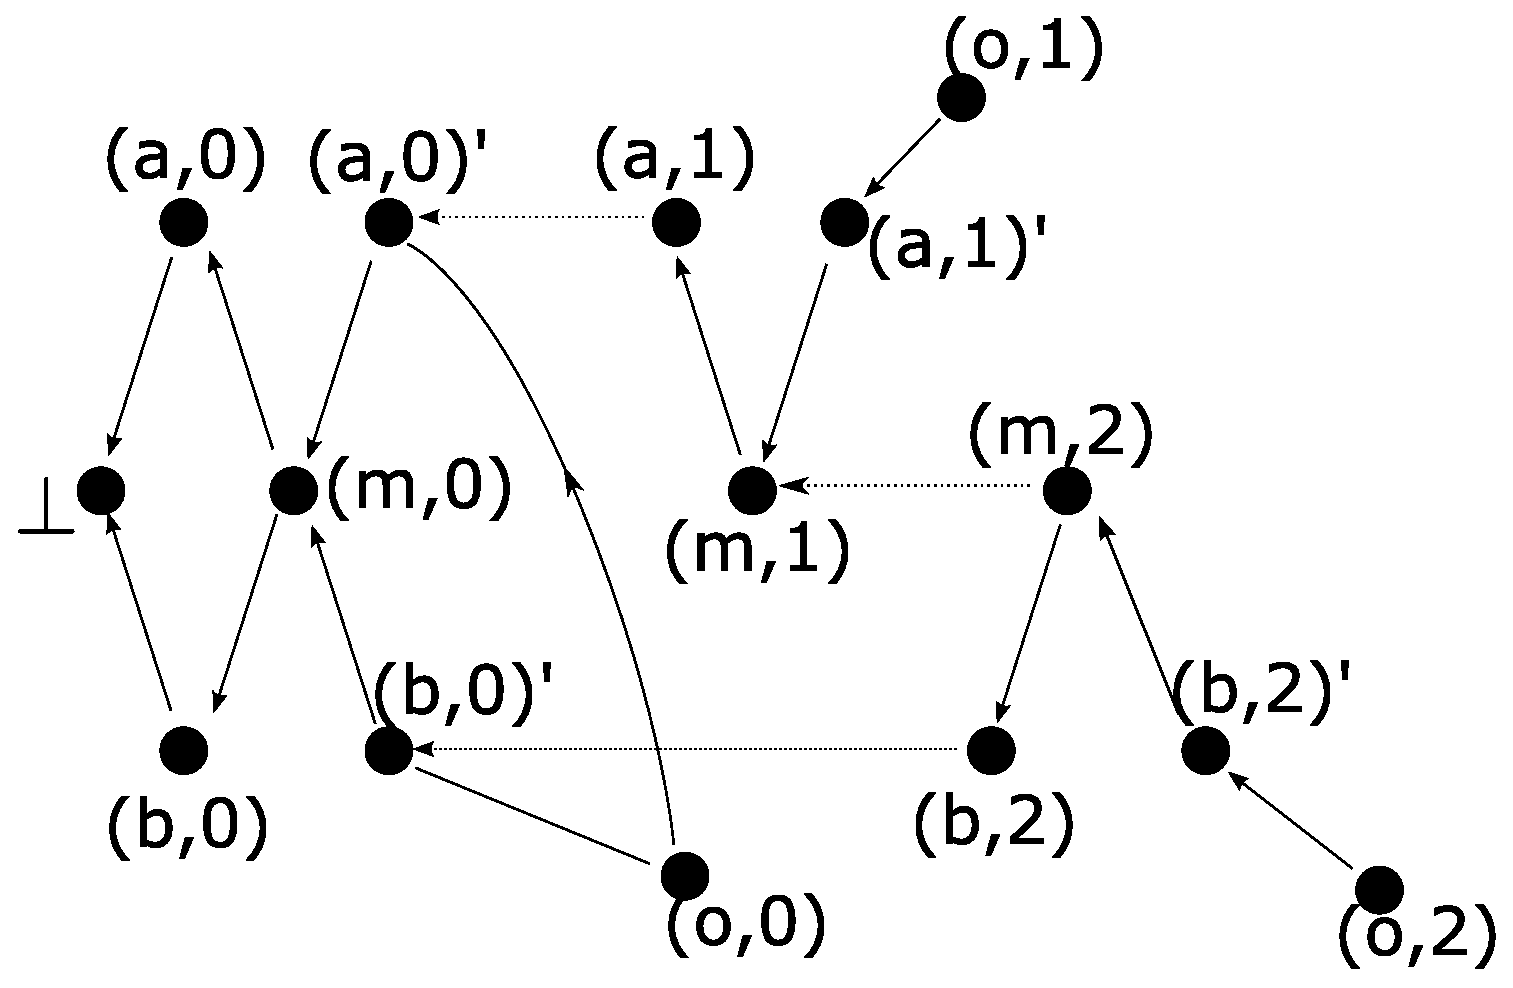
\includegraphics[scale=0.3]{schedulemodel.eps} 
\end{center}
\caption[A model $R(\cdot, \sigma)$.]{A model $R(\cdot, \sigma)$
 induced by the partial schedule $\sigma = \left(\{a,b\}, \{a\}, \{b\}\right)$.
 A solid arrow pointing to $(x,n)$ shows an $f_x$ mapping.  Dotted arrows show $\preceq$ relations.
 We omit implied arrows and the valuation.}
 \label{schedulemodel}
\end{figure}

We can state the logical characterisation of waitfree communication.
\begin{theorem}[Completeness for waitfree communication]
\label{wf:sc-comp}
 Assume $\varphi\supset \psi$ is a waitfree assertion.
 The relation $\vdash_{SC} \varphi\supset\psi$ holds if the relation $R(\varphi, \sigma),
 (o,n) \models \psi$ holds for any compatible partial schedule $\sigma$ where the state~$(o,n)$
 is the last state of the waitfree model $R(\varphi, \sigma)$.
\end{theorem}
To prove completeness, we only use special models called singleton
models induced by a permutation of processes.

\begin{definition}
 For a set of processes $P$, we define $\mathsf S(P)$ to be the set of the permutations of $P$.
\end{definition}

\begin{definition}
 For $\pi\in \mathsf S(P)$ and $0\le k\le |P|$, we define
 $SC(\pi,k)$ to be the set $\{K_\memory K_a I_a\supset K_\memory K_b I_b\mid b\le a\mbox{ in }\pi_0,\ldots \pi_k\}$.
\end{definition}

\begin{lemma}
 \label{perm}
 $\vdashsc \bigvee_{\pi\in \mathsf S(A)} SC(\pi, |P|)$ holds.
\end{lemma}
\begin{proof}
 It suffices to use rule (SC) many times.
\end{proof}

\begin{definition}
 For a permutation $\pi$ of $P$ and a waitfree protocol description $\varphi$, we
 define a partial schedule $\sigma(\varphi, \pi)$ as
\[
 \sigma(\varphi, \pi) = 
 \overbrace{\pi_0, \cdots, \pi_0}^{count_{\pi_0}(\varphi)},
 \overbrace{\pi_1, \cdots, \pi_1}^{count_{\pi_1}(\varphi)},
 \cdots \cdots
 \cdots,
 \overbrace{\pi_n,\cdots, \pi_n}^{count_{\pi_n}(\varphi)}.
\]
\end{definition}

\begin{definition}
 A singleton model is a model of the form $R(\varphi, \sigma(\varphi,
 \pi))$. We abbreviate this to $R(\varphi, \pi)$.

 For a singleton model and an index $k\in I$, $w_k$ denotes the minimum external
 observer state above all $\pi_j$~states for $j< k$.
\end{definition}

\begin{definition}
 For a waitfree protocol description $\varphi = \bigwedge_{a\in A} 
 \overbrace{K_a K_\memory K_a \cdots K_a}^{n_a}
 I_a$, we define the restriction \\
 $\varphi\restriction_{p,k} = 
 \bigwedge_{a\in A\restriction_{p,k}} \overbrace{K_a K_\memory K_a \cdots K_a}^{n_a} I_a$,
 where $A\restriction_{p,k} = \{a\mid p_j = a \mbox{ for some
 } j<
 k\}$.
\end{definition}

\begin{lemma}
 \label{stronger}
 $R(\varphi, \pi), (o,k)\models \psi\Longrightarrow SC(\pi, k)\vdash
 \varphi\restriction_{\pi,k}\supset\psi$.
\end{lemma}
\begin{proof}[Proof of Lemma~\ref{stronger}]
 By induction on $k$.
\begin{description}
 \item[(Case $k=0$)] 
 We show a stronger proposition:
$
 (o,0)\models \psi \quad\Longrightarrow\quad f_{p_0}(o,0)\models \psi,
 \vdash \varphi\restriction_{p,0}\supset \psi
 \mbox{ and }
 \vdash \varphi\restriction_{p,0}\supset K_a\psi.
$
by inner induction on $\psi$.
\begin{description}
 \item[(When $\psi$ is an atomic formula $P$)] 
 $P = I_{\pi_0}$ holds.
 Since $\varphi\restriction_{\pi,0} = K_{\pi_0}K_\memory K_{\pi_0}\cdots K_\memory K_{\pi_0}I_{\pi_0}$,
 $\vdash\varphi\restriction_{\pi,0}\supset K_{\pi_0}P$ holds.
 So, $SC(\pi,0)\vdash \varphi\restriction_{\pi,0}\supset K_{\pi_0}P$ holds.
 Consequently, $SC(\pi,0)\vdash \varphi\restriction_{\pi,0}\supset P$ also holds.
 \item[(When $\psi = \psi_0\wedge \psi_1$ or $\psi_0\vee\psi_1$)] 
 Induction goes smoothly.
 \item[(When $\psi = K_a\psi'$)]
 Assume $(o,0)\models K_a\psi'$. Claim: $a=\pi_0$ holds.
 Seeking contradiction, assume $a\neq \pi_0$.
 That means $f_a(o,0) = \bot$.
 However, waitfree task specification is satisfied at the state $\bot$.
 Contradiction.
 We have proved $a=\pi_0$. Using this, we can show that $f_a(o,0)\models\psi'$ holds.
 By idempotency of $f_a$, $f_a(f_a((o,0)))\models \psi'$ holds.
 This means $f_a((o,0))\models K_a\psi'$.
 Since $(o,0)\models \psi'$, by inner induction hypothesis,
 $\vdash \varphi\restriction_{\pi,0}\supset K_a\psi_a'$.
 By proof theoretic consideration,
 $\vdash \varphi\restriction_{\pi,0}\supset K_a K_a\psi'$ holds.
\end{description}
 \item[(Case $k = k' + 1$)]
 Like the base case, we show a stronger proposition
$
 (o,k)\models \psi\Leftrightarrow f_{\pi_k}((o,k))\models \psi \Rightarrow SC(\pi,k)\vdash
 \varphi\restriction_{\pi,k}\supset \psi\mbox{ and }SC(\pi,k)\vdash
 \varphi\restriction_{\pi,k}\supset K_{\pi_k}\psi, 
$
using induction on $\psi$.
\begin{description}
 \item[(When $\psi = P$, an atomic formula)] 
 Either $R(\varphi, \pi), w_{k'}\models P$ or $I_{\pi_k}=P$ holds.
 In the former case, by induction hypothesis.
 In the latter case, similarly as the base case.
 \item[(When $\psi = \psi_0\wedge \psi_1$ or $\psi_0\vee\psi_1$)] 
 Induction goes smoothly.
 \item[(When $\psi = K_x\psi'$)] 
If $\pi_k\neq x$, $f_{\pi_k}((o,k))\models K_x\psi'$ implies $(o,k')\models K_x\psi'$.
	    By outer induction hypothesis, $SC(\pi,k')\vdash
	    \varphi\restriction_{\pi,k'}\supset K_x\psi'$ and
	    $SC(\pi,k')\vdash \varphi\restriction_{\pi,k'}\vdash
	    \varphi\restriction_{\pi,k'}\supset K_x\psi'$ hold.
	    Here, we can safely replace $k'$ with $k$.
	    If $\pi_k=x$, $(o,k)\models K_x\psi'$ imply
	    $(o,k)\models \psi'$.
	    By inner induction hypothesis, we obtain
	    $SC(\pi,k)\vdash\varphi\restriction_{\pi,k}\supset K_x\psi'$.
	    This also implies $SC(\pi,k)\vdash\varphi\restriction_{\pi,k}\supset K_xK_x\psi'$.
\end{description}
\end{description}
\end{proof}
After showing this generalised lemma, proving Theorem~\ref{wf:sc-comp} is
easy.
\begin{proof}[Proof of Theorem~\ref{wf:sc-comp}]
 Since $R(\varphi, p), w_{|P|}\models \psi$, $SC(p,|P|)\vdash \varphi\supset
 \psi$.
By Lemma~\ref{perm}, $\vdashsc
 \varphi\supset \psi$.
\end{proof}
Any models induced by a partial schedule is finite.  For a waitfree assertion $\varphi$,
it is decidable whether $\vdashsc \varphi$ holds or not.


\subsection{Decidability of Solvability of Waitfree Task Specification}

\begin{definition}
 A waitfree task specification $\psi$ is solvable if there is such a
 waitfree protocol description $\varphi$ that the relation
 $R(\varphi,\sigma), (o,n)\models\psi$ holds for any compatible partial
 schedule $\sigma$ where the state $(o,n)$ is the last state of the
 model $R(\varphi,\sigma)$.
\end{definition}

\noindent \textbf{Fact.} The set of solvable waitfree task specifications are
recursively enumerable because the relation $\vdashsc$ is axiomatised.

\noindent \textbf{Fact.} The set of unsolvable waitfree task
specifications are recursively enumerable because partial schedule-induced
models are recursively enumerable.

\begin{theorem}
 \label{wf-dec}
 It is decidable whether a waitfree task
specification is solvable or not.
\end{theorem}
\begin{proof}
These two facts imply that it is decidable whether a waitfree task
specification is solvable or not.
\end{proof}

This does not contradict to the undecidability
 of waitfreely solvable tasks by Gafni and
 Koutsoupias~\cite{gafni1999three}
 because the undecidability proof
utilises tasks that cannot be expressed by waitfree task specifications.
They use tasks involving consensus:
the tasks involving making agreements among processes, where
whether an output value is allowed or not depends on other processes'
output values.  Waitfree task specifications cannot describe such tasks.

\section{Related Work}
\label{first:related}

Van Benthem~\cite{van2009information} investigates the connection between
intuitionistic logic and information dynamics.  He speculates:
\begin{quotation}
It might be
that intuitionistic logic points the way towards a grand synthesis of information analysis
in the standard model-theoretic style with the dynamic view of logic as embodied
in proof and games.
\end{quotation}
This paper replies his speculation by defining knowledge in terms of BHK-interpretation
and defining a proof system \iec\,embodying the interpretation.

Ondrej Majer's 
Epistemic Logic with Relevant Agents~\cite{majer-epistemic}
is similar to \iec\, in that both logics have epistemic modalities and that both logics are
not classical.
However, the logic given in~\cite{majer-epistemic}
 contains only one modality $K$ for knowledge.
This implicitly assumes that there is a single agent, not multiple agents so that it is
impossible for their logic to treat communication between multiple agents.

Many logics have both temporal and epistemic modalities~\cite{sato13study, wozna2005logic}.
Ewald~\cite{1986} proposes an intuitionistic logic with temporal modality.
We unify the intuitionistic semantics and temporal semantics so that the logic
\iec\,lacks temporal modality yet represents some temporal notions.
Adding a temporal modality like Ewald~\cite{1986} would increase the expressivity of the
logic, but it would complicate the syntax and semantics.
We would like to investigate the simple logic \iec\,first
 and then expand \iec\,with
additional constructs.

In Kobayashi and Yonezawa's logic~\cite{kobayashi1995asynchronous}, processes
appear in formulas but time does not appear in formulas
because time is implicit in the system of logic programming.
This logic is different from \iec\, in that this logic is based on linear logic and that their
usage is logic programming.

Belnap and Harper's ``seeing to it that'' (stit) logical operator
aims at describing interaction between agents.
The semantics for the operator involves both agency and temporal notion, which is more
complicated than the meaning of $K_a$ operator in \iec.
A fundamental difference of the stit operator and the epistemic operator in \iec\,
is whether the modalities mention the future or tha past.
The stit operator mentions the future while the epistemic operator mentions the past.

Dynamic epistemic logic is a logic that aims at reasoning about communication.
However the semantics of the logic involves
instantaneous change of models.
We argue such instantaneous change of the whole world it is
not a natural description of asynchronous communication.


\section{Conclusion}
\label{conclusion}


On the logic~\iec, we analysed the concept of sequential consistency and wait-free
communication.
The depth of our anlaysis is represented in a deep proof tree (Figure~\ref{hoge}) for a
property of a relatively simple and small wait-free protol involving two processes.
Distributed programming over shared memory can be seen as a game involving the scheduler
and the program.
Logic can be seen as a game involving the models and the formulas.
We modelled schedules as a model of logic and programs as formulas.
Since sequential consistency is a restriction on schedules,
we modeled sequential consistency as a restriction on models.
The restriction on the models representing sequential consistency could actually
axiomatized using an axiom type that is similar to the axiom type for prelinerity defining
a famous intermediate logic.
Since waitfreedom is a restriction on programs,
we modelled waitfree programs as a set of formulas called waitfree protocol description.
We also modelled specification for waitfree programs as a set of formulas called waitfree
task specification.
We used a waitfree assertion, which is
an implication formula consisting of a waitfree protocol description and a
waitfree task specification,
 to represent
an assertion that a waitfree protocol meets a specification.




\chapter{Finite Model Property for Sequential Consistency Logic}


\section{Introduction}

We proved finite model property for sequential consistency logic
using analytic tableaux.
The target logic have Kripke frames where modalities are interpreted as
functions over the frame.  Moreover, each logic is parametrized by a
set of restrictions.  Each restriction is a disjunction of some
inequalities posing restrictions on the shape of the frame.

The target class of intermediate modal logics is a generalization of
intuitionistic epistemic logic proposed by Hirai~\cite{hirailpar}.
He used intuitionistic epistemic logic in order to model shared memory
consistencies, which are criteria that guarantees levels of
synchronization among different processes.
Both shared memory consistencies and some intermediate modal logics
can be characterized as a restriction on
partially-ordered structure:
Kripke frames for intermediate modal logics
and executions for shared memory
consistencies~\cite{steinke2004unified}.
He regarded Kripke frames as executions in order to translate
an intermediate modal logic into a shared memory
consistency.

However, he did not show finite model property for those
intermediate modal logics.  When software engineers talk about shared
memory consistencies, they assume an execution is finite.
When we think of Kripke models as executions, we are obliged to show
that the model is finite.
Especially when we want to construct a specific counterexample execution,
we have to build a \textit{finite} Kripke model.

For example,
under \textit{sequential consistency logic}, which is intuitionistic epistemic
logic along with the axioms of the form
$(K_m\varphi\supset K_m\psi) \vee (K_m\psi\supset K_m\varphi)$,
the formula $K_aK_mK_aI \supset K_bK_mK_bJ\supset K_bI$ is not a
theorem.
In terms of shared memory consistency, this means that even when a
process~$a$ has put information~$I$ on the shared memory and got a
successful acknowledgement from the shared memory and the other
process~$b$ does the same with information~$J$, it is not always the
case that process~$b$ has obtained information~$I$\kern -2pt.
In other words, there are executions without this property.
This can be confirmed via
finite model property for sequential consistency logic.
We show this property in a generalized form.

\section{The Target Logics}
 \label{logic}

The class of logics that we consider is a generalization of
intuitionistic propositional logic.
The class of logics also contains G\"{o}del--Dummett logic~\cite{dummett59}
and the intuitionistic epistemic logic proposed by 
Hirai~\cite{hirailpar}.
Let us assume that
there are a countably infinite set~$\pvar$ of \textit{propositional variables} and a 
finite set~$\agents$ of \textit{agents}. 

\begin{definition}
We define the set~$\fml$ of formulas by BNF:
\[
 \varphi,\psi ::= \bot\mid I\mid K_a\varphi\mid (\varphi\vee\psi)\mid
 (\varphi\wedge\psi)\mid (\varphi\supset\psi)
\]
 where $a$ is an agent in $\agents$
 and $I$ is a propositional variable in~$\pvar$.
\end{definition}

For a set of formulas $\Gamma\!$, notation $K_a\Gamma$ denotes the set
$\{K_a\varphi\mid\varphi\in\Gamma\}$\enspace.

\begin{definition}[Kripke frame]
A \textit{frame} $\tuple{W,\preceq,(f_a)_{a\in \agents}}$ is a tuple where
\begin{itemize}
 \item $\tuple{W,\preceq}$ is a partially ordered set, and
 \item each $f_a\colon W\rightarrow W$ is a monotonic function with
       respect to~$\preceq$.
\end{itemize} 
\end{definition}

\begin{definition}[Kripke model]
A \textit{model} $\tuple{W,\preceq, (f_a)_{a\in \agents},\rho}$ is a tuple where
\begin{itemize}
 \item $\tuple{W,\preceq,(f_a)_{a\in \agents}}$ is a frame, and
 \item $\rho\colon \pvar\rightarrow 2^W$ is a function that maps every
       propositional variable to a upward-closed subset of $W\!$.
\end{itemize}
\end{definition}

We are going to prove finite model property for a class of
intermediate modal logics.  The logics are parametrized with
world restriction sets,  which we are going to define.
We assume that there is a countably infinite set of \textit{world
variables}~$\wvar$.
We use $\mathsf v, \mathsf w,\ldots$ to denote world variables.
We define \textit{world terms} using BNF:
\[
 \mathsf s::=\mathsf v\mid \mathsf s.a
\]
where $a$ is an agent.
Every world term can be written as $\mathsf v.s$ where $s$ is a fintie sequence
of agents (a postfix).
A \textit{world inequality} is an inequation of the form $\mathsf s\le
\mathsf t$ where $\mathsf s$ and $\mathsf t$ are world terms.
\begin{definition}
A world restriction is a sequence of world inequalities jointed
 by~$\wor$ formed like
 $\mathsf v_0.s_0\le\mathsf v_1.t_1\wor\cdots\wor
 \mathsf v_{n-1}.s_{n-1}\le\mathsf v_n.t_n\wor \mathsf v_n.s_n\le\mathsf
 v_0.t_0$ that satisfies either
 \begin{itemize}
  \item (single clause) $n=0$, or
  \item (single postfix) $s_i = t_i = s_j = t_{j}$ for $0\le i,j\le n$.
 \end{itemize}
\end{definition}
A \textit{world restriction set} is a finite set of world restrictions.

A \textit{world valuation} maps a world variable into a world of a frame.
We extend a world valuation on world variables
$\delta\colon\mathcal V_W\rightarrow W$ to that on world terms
inductively as $\delta(\mathsf s.a)=f_a(\delta(\mathsf s))$.
A frame $\tuple{W,\preceq, 1,(f_a)_{a\in\agents}}$ satisfies a world inequality
$\mathsf s\le\mathsf t$ iff $\delta(\mathsf s)\preceq \delta(\mathsf t)$
for all $\delta\colon\mathcal V_W\rightarrow W$.
A frame~$F$ satisfies a world restriction $\mathsf r$
iff $M$ satisfies $\delta(\mathsf r)$ for any world valuation~$\delta$.
For example, a frame satisfies $\mathsf v\le \mathsf w\wor\mathsf
w\le\mathsf v$ iff the frame is totally ordered.
An $\mathsf R$-frame is a frame that
satisfies all world restrictions in~$\mathsf R$.
An $\mathsf R$-model is a model with an $\mathsf R$-frame.


\begin{definition}
 We define the \textit{validity relation} $M,w\models\varphi$ over a model
 $M = \tuple{W,\preceq,(f_a)_{a\in \agents},\rho}$, a state~$w\in W$ and a
 formula~$\varphi$ inductively on $\varphi$.
 In this definition, let
 us abbreviate $M,w\models \varphi$ into $w\models \varphi$\enspace.
\newcommand{\m}{}
\begin{itemize}
\item $w\models \bot$ never holds.
\item $w\models I$ iff
$w \in
 \rho(I)$.
\item	    $w\models K_a \psi$ iff
	    $f_a(w)\models \psi$.
\item $w\models \psi_0\wedge\psi_1$ iff both
 $w\models \psi_0$ and $w\models \psi_1$ hold.
\item
 $ w\models \psi_0\vee\psi_1$ iff either
 $ w\models \psi_0$ or $w\models \psi_1$ holds.
\item
	   $w\models \psi_0\supset\psi_1$ iff 
	   $w'\succeq w$ and $w'\models \psi_0$ imply
	   $w'\models\psi_1$ for any $w'\in W$\enspace.
\end{itemize}
\end{definition}
A model~$M$ \textit{satisfies} $\varphi$ iff $M,w\models\varphi$ holds for any
state~$w$ of~$M$.
A formula~$\varphi$ is \textit{valid under} $\mathsf R$ iff
every $\mathsf R$-model~$M$ satisfies $M\models \varphi$.
For this, we write $\modelsR \varphi$\enspace.

\begin{lemma}[Kripke monotonicity]
 \label{monot}
 $M,w\models\varphi$ and $w\preceq v$ imply 
$M,v\models\varphi$.
\end{lemma}
\begin{proof}
 Induction on~$\varphi$.
 We use monotonicity of $f_a$ here.
\end{proof}

\paragraph{The proof system.}
Since both $\pvar$ and $\wvar$ are countably infinite,
there is an injection that maps a world variable to a propositional
variable.
We fix one such injection
$\mathsf w\mapsto I_{\mathsf w}$.
Inductively on the construction of world terms,
we assign a formula~$[\mathsf t]$ to every world term~$\mathsf t$:
\begin{itemize}
 \item for a world term $\mathsf w\in \wvar$, we define $[\mathsf w]$ to be
       $I_{\mathsf w}$,
 \item for a world term $\mathsf{s.a}$, we construct
 a formula $[\mathsf{s.a}]$ by
replacing every propositional variable~$P$ with $K_aP$ in $[\mathsf s]$.
\end{itemize}
Note that the sequence $\mathsf{.a.b.c}$ is translated into the same
order $K_a K_b K_c$ although a postfix is translated into a prefix.
We define $K_s\varphi$ as $[\mathsf w.s][\varphi/I_{\mathsf w}]$.
Also, we define $f_b\circ f_a$ as $f_{ab}$.  This ensures $M, w\models
K_s\varphi\Leftrightarrow M,f_s(w)\models\varphi$.

This translation of world terms into formulas
enables us to translate world inequalities and world restrictions
into formulas:
\begin{itemize}
 \item $[\mathsf s\le \mathsf t] := [\mathsf s]\supset [\mathsf t]$, and
 \item $[\mathsf{s_0}\le \mathsf{t_0}\wor \cdots\wor \mathsf{s_n}\le \mathsf{t_n}] := [\mathsf{s_0}\le \mathsf{t_0}]\vee
       \cdots \vee [\mathsf{s_n}\le \mathsf{t_n}]$ \enspace.
\end{itemize}

We define $\mathbf{Ax}(\mathsf R)$ to be the substitution closure of
$\{[\mathsf r]\mid \mathsf r\in \mathsf R\}$.
The substitution closure of a set~$S$ of formulas is defined as
$\{\varphi[\psi/P]\}$ where $\psi$ run freely on~$\fml$ and $P$ on~$\pvar$.

\begin{figure}[t]
\begin{center}
 \def\fCenter{\vdashR}
\AxiomC{}
\LeftLabel{(axiom)}
\UnaryInf$\varphi \fCenter \varphi$
 \DisplayProof
\hfill
\Axiom$\Gamma\fCenter\varphi$
\LeftLabel{(weakening)}
 \UnaryInf$\psi,\,\Gamma\fCenter\varphi$
\DisplayProof
 \hfill
\Axiom$ \varphi,\,\varphi,\,\Gamma\fCenter\psi$
\LeftLabel{(contraction)}
\UnaryInf$\varphi,\,\Gamma\fCenter\psi$
\DisplayProof
\ruleskip
\Axiom$\Gamma, \varphi,\psi,\, \Gamma'\fCenter\theta$
\LeftLabel{(exchange)}
\UnaryInf$\Gamma,\,\psi,\varphi,\,\Gamma'\fCenter\theta$
\DisplayProof
\hfill
\Axiom$\Gamma\fCenter\varphi$
\Axiom$\Gamma'\fCenter\psi$
\LeftLabel{($\wedge$-I)}
\BinaryInf$\Gamma,\Gamma'\fCenter \varphi\wedge\psi$
\DisplayProof
\hfill
\Axiom$\Gamma\fCenter \varphi$
\LeftLabel{($\vee$-I$_0$)}
\UnaryInf$\Gamma\fCenter \varphi\vee\psi$
\DisplayProof
\ruleskip
\Axiom$\Gamma\fCenter \varphi$
\LeftLabel{($\vee$-I$_1$)}
\UnaryInf$\Gamma\fCenter \psi\vee\varphi$
\DisplayProof
\hfill
\Axiom$\Gamma \fCenter\varphi\wedge\psi$
\LeftLabel{($\wedge$-E$_0$)}
\UnaryInf$\Gamma\fCenter \varphi$
\DisplayProof
\hfill
\Axiom$\Gamma\fCenter \varphi\wedge\psi$
\LeftLabel{($\wedge$-E$_1$)}
\UnaryInf$\Gamma\fCenter \psi$
\DisplayProof
\ruleskip
\Axiom$\Gamma\fCenter \psi_0\vee\psi_1$
\Axiom$\Gamma,\,\psi_0\fCenter \varphi$
\Axiom$\Gamma,\,\psi_1\fCenter \varphi$
\LeftLabel{($\vee$-E)}
\TrinaryInf$\Gamma\fCenter \varphi$
\DisplayProof
\vskip 5mm
\Axiom$\varphi,\,\Gamma\fCenter\psi$
\LeftLabel{($\supset$-I)}
\UnaryInf$\Gamma\fCenter \varphi\supset\psi$
\DisplayProof
\hfill
\Axiom$\Gamma\fCenter\psi_0\supset\psi_1$
\Axiom$\Gamma\fCenter \psi_0$
\LeftLabel{($\supset$-E)}
\BinaryInf$\Gamma\fCenter \psi_1$
\DisplayProof
\hfill
\Axiom$\Gamma\fCenter\bot$
 \LeftLabel{($\bot$-E)}
 \UnaryInf$\Gamma\fCenter\varphi$
 \DisplayProof
\ruleskip
\AxiomC{}
\LeftLabel{($\vee K$)}
 \UnaryInf$K_a(\varphi\vee\psi)\fCenter (K_a \varphi)\vee K_a\psi$
\DisplayProof
 \hfill
 \AxiomC{}
 \LeftLabel{($\varphi\in \mathbf{Ax}(\mathsf R)$)}
 \UnaryInf$\fCenter\varphi$
 \DisplayProof
 \ruleskip
 \Axiom$\Gamma\fCenter\varphi$
 \LeftLabel{(necessitation)}
 \UnaryInf$K_a\Gamma\fCenter K_a\varphi$
 \DisplayProof
\end{center}
\caption{Deduction rules of $\vdashR$.}
\label{figR}
\end{figure}

\begin{definition}
 We define the proof system $\vdashR$ by Fig.~\ref{figR}.
\end{definition}

\begin{theorem}
 \label{sound-comp-nat-kripke}
 $\Gamma\vdashR\varphi\Longleftrightarrow\Gamma\modelsR \varphi$\enspace.
\end{theorem}
\begin{lemma}[Soundness]
 $\Gamma\modelsR\varphi\Longleftarrow\Gamma\vdashR\varphi$
\end{lemma}
\begin{proof}
We show $\Gamma\modelsR\varphi$ inductively
on the definition of $\Gamma\vdashR\varphi$.
\begin{description}
 \item[(Case {Ax})]
	    Suppose $\varphi\in \mathsf{Ax}(R)$.
	    For an $\mathsf{R}$-model~$M$ and a state~$w$ of~$M$,
	    we are going to show $M,w\models\varphi$.
	    Seeking contradiction,
	    we assume $M,w\not\models\varphi$.
	    Since $\varphi\in\mathsf{Ax}(R)$, there exists a world
	    restriction $\mathsf r\in\mathsf R$ with
	    $\varphi=[\mathsf r]\theta$,
	    where $\theta$ is a substitution.
	    Let $\mathsf r$ be
	    $\mathsf v_0.s_0\le\mathsf v_1.t_1\wor\cdots\wor
	    \mathsf v_{n-1}.s_{n-1}\le\mathsf v_n.t_n\wor\mathsf
	    v_n.s_n\le\mathsf v_0.t_0$.
	    Then,
	    $\varphi = (K_{s_0}\varphi_0\supset
	    K_{t_1}\varphi_1)\vee\cdots\vee
	    (K_{s_{n-1}}\varphi_{n-1}\supset K_{t_n}\varphi_n)
	    \vee (K_{s_n}\varphi_n\supset K_{t_0}\varphi_0)$
	    for some $(\varphi_i)_{0\le i\le n}$.
	    We define $\varphi_{n+1}$ to be $\varphi_0$ and
	    $\varphi_{-1}$ to be $\varphi_n$.
	    By assumption, $M,w\not\models K_{s_i}\varphi_i\supset
	    K_{t_{i+1}}\varphi_{i+1}$ for any $0\le i\le n$.
	    This implies existence of a sequence
	    $(v_i)_{0\le i\le n}$ of states with $w\preceq v_i$ and
	    $M,v_i\models K_{s_i}\varphi_i$ but $M,v_i\not\models
	    K_{t_{i+1}}\varphi_{i+1}$.
	    By the semantics of modalities, we have
	    $M,f_{s_i}(v_i)\models \varphi_i$ but $M,
	    f_{t_{i+1}}(v_i)\not\models\varphi_{i+1}$
	    for any $0\le i\le n$.
	    When $\mathsf r$ is single clause,
	    $\mathsf r = \mathsf v.s\le\mathsf v.t$.
	    Let $\delta(\mathsf v)$ be $v_0$.
	    Since $M$ is an $\mathsf R$-model,
	    $f_s(v_0)\preceq f_t(v_0)$ holds.
	    Since $n=0$,
	    we have $M,v_0\models K_s\varphi_0$ but $M,v_0\not\models
	    K_t\varphi_0$.
	    This contradicts Kripke monotonicity.
	    Otherwise, when $\mathsf r$ is single postfix,
	    $\mathsf r = \mathsf v_0.s\le\mathsf
	    v_1.s\wor\cdots\wor\mathsf v_{n-1}.s\le\mathsf
	    v_n.s\wor\mathsf v_n.s\le\mathsf v_0.s$.
	    Let $\delta(\mathsf v_i)$ be $v_{n-i}$.
	    Since $M$ is an $\mathsf R$-model,
	    for some $0\le i\le n$,
	    we have $\delta(\mathsf v_i.s)\preceq \delta(\mathsf
	    v_{i+1}.s)$.
	    This is equivalent to $f_s(v_{n-1})\preceq f_s(v_{n-i-1})$.
	    The way we took $(v_i)_{0\le i\le n}$ ensures
	    $M,v_{n-1}\models K_s\varphi_{n-i}$.
	    In other words, $M,f_s(v_{n-1})\models \varphi_{n-i}$.
	    By Kripke monotonicity, $M,f_s(v_{n-i-1})\models
	    \varphi_{n-i}$.
	    This contradicts $M,f_s(v_{n-i-1})\not\models\varphi_{n-1}$.
 \item[(Other rules)]
	    Straightforward.
\end{description}
\end{proof}

\subsection{Examples}

\paragraph{Classical logic.}
When
$\mathsf R = \{\mathsf v\le\mathsf w\wor\mathsf w\le\mathsf x\wor\mathsf x\le\mathsf
v\}$,
the corresponding axioms can be obtained as follows:
\begin{align*}
[ \mathsf v\le \mathsf w\wor \mathsf w\le\mathsf x\wor \mathsf x\le\mathsf v ] &=
(I_{\mathsf v}\supset I_{\mathsf w})\vee (I_{\mathsf w}\supset
I_{\mathsf x})\vee (I_{\mathsf x}\supset I_{\mathsf v})
\\
\mathbf{Ax}(\mathsf R) = \mathbf{Ax}(\{\mathsf v\le\mathsf w\wor \mathsf
w\le \mathsf x \wor \mathsf x\le\mathsf v\}) &= \{(\varphi\supset\psi)\vee(\psi\supset\chi)\vee(\chi\supset\varphi)\}.
\end{align*}
$\mathbf{Ax}(\mathsf R)$ is equivalent to the excluded middle so $\mathsf R$ defines
classical logic.

\paragraph{G\"{o}del--Dummett logic.}
When $\mathsf R=\{\mathsf v\le\mathsf w\wor\mathsf w\le\mathsf v\}$,
the corresponding axioms can be obtained as follows:
\begin{align*}
[\mathsf v\le \mathsf w\wor \mathsf w\le\mathsf v] &=
(I_{\mathsf v}\supset I_{\mathsf w})\vee (I_{\mathsf w}\supset
I_{\mathsf v})\\
\mathbf{Ax}(\mathsf R) = \mathbf{Ax}(\{\mathsf v\le\mathsf w\wor \mathsf
w\le \mathsf v\}) &= \{(\varphi\supset\psi)\vee(\psi\supset\varphi)\mid
\varphi,\psi\colon\mbox{formula}\}.
\end{align*}
$\mathbf{Ax}(\mathsf R)$ coincides with the axioms of
G\"{o}del--Dummett logic~\cite{dummett59}.

\paragraph{Sequential consistency logic.}
When $\mathsf R=\{\mathsf v.\mathsf m\le\mathsf w.\mathsf m\wor \mathsf
w.\mathsf m\le \mathsf v.\mathsf m\}$,
the corresponding set of axioms
$\mathbf{Ax}(\mathsf R) = \{(K_{\mathsf m}\varphi\supset K_{\mathsf
m}\psi)\vee(K_{\mathsf m}\psi\supset K_{\mathsf m}\varphi)\mid \varphi,
\psi\colon\mbox{formula}\}$
 axiomatizes sequential consistency logic,
which is proposed by Hirai~\cite{hirailpar} for modeling a shared memory consistency called sequential consistency.


\section{Finite Model Property}
\label{fmp-proof}

This is our main result.
\begin{theorem}
 \label{thm:fmp}
 $\vdashR\varphi$ holds iff $M\models \varphi$ holds
 for all finite {\sf R}-model $M$.
\end{theorem}

We use another deduction system\,\LB\,in order to obtain finite model
property.
The outline of the proof is these circular implications:
\begin{align*}
 \vdashRLB\varphi &\Longrightarrow \quad \models_{\mathsf R}\varphi\quad
 &(\mbox{by Lemma~\ref{sound}})\\
 &\Longrightarrow \quad \vdash_{\mathsf R}\varphi &(\mbox{by
 Thm.~\ref{sound-comp-nat-kripke}}) \\
 &\Longrightarrow\quad \modelsR\varphi &\mbox{(by Thm.~\ref{sound-comp-nat-kripke})}\\
 &\Longrightarrow\quad M\models\varphi \mbox{ for any finite $\mathsf
 R$-model }M\\
 &\Longrightarrow\quad \vdashRLB\varphi & (\mbox{by
 Lemma~\ref{R-fmp}})\enspace .
\end{align*}
This method extends Waaler
and Wallen's method for intuitionistic logic~\cite{waaler1999tableaux}.

\subsection{\LB}

The deduction system\,\LB\,uses \textit{prefixed formulas}.  A
prefixed formula is shaped like $\mathsf s::\varphi$ where $\mathsf s $
is a world term and $\varphi$ is a formula.
Informally, this prefixed formula means that the formula~$\varphi$ is
satisfied in a state referenced by~$\mathsf s$.
A \textit{sequent} is shaped like
  $\Theta\parallel \Gamma\longrightarrow \Delta$ where
$\Theta$ is a finite set of world inequalities and both
$\Gamma$ and $\Delta$ are finite sets of prefixed formulas.
In a sequent, world inequality
$\mathsf s\le \mathsf s$ must be in $\Theta$
 for any world term $\mathsf s$ occurring in $\Delta$ or $\Gamma$.

A set~$\Theta$ of world inequalities
\textit{conforms to} world restriction set~$\mathsf R$ when all of the
following hold:
\begin{itemize}
 \item $\mathsf s\le \mathsf t, \mathsf t\le \mathsf u\in
       \Theta\Longrightarrow
       \mathsf s\le \mathsf u\in\Theta$,
 \item If $\mathsf{s_0}\le \mathsf{t_0} \wor \mathsf{s_1}\le \mathsf
       {t_1}\wor
       \cdots\wor \mathsf{s_n}\le
       \mathsf{t_n}\in \bar{\mathsf R}$ and all of
       $\mathsf{s_0},\mathsf{s_1},\ldots,\mathsf{s_n},
       \mathsf{t_0},\mathsf{t_1},\ldots, \mathsf{t_n}$ appear in~$\Theta$, then,
       $\mathsf{s_i}\le \mathsf{t_i}\in\Theta$ for at least
       one~$\mathsf{i}$, where $\bar {\mathsf R}$ is the substitution
       closure of~$\mathsf R$,
 \item If $\mathsf s\le\mathsf t\in\Theta$ and both $\mathsf s.a$ and
       $\mathsf t.a$ appear in~$\Theta$, then $\mathsf s.a\le\mathsf
       t.a\in \Theta$.
\end{itemize}
We define $\mathsf R(\Theta)$ to be the set of the minimal
supersets of~$\Theta$ conforming to~$\mathsf R$.
For example, when $\mathsf R=\{\mathsf w\le \mathsf v\wor\mathsf v\le \mathsf
w\}$,
$\mathsf R(\{\mathsf w\le \mathsf w, \mathsf v\le \mathsf v\}) =
\{\{\mathsf w\le \mathsf v, \mathsf w\le \mathsf w, \mathsf v \le
\mathsf v\}, \{\mathsf v \le
\mathsf w, \mathsf w\le \mathsf w, \mathsf v\le \mathsf v\}\}$\enspace.
 When $\Theta$ is finite, so is $\mathsf R(\Theta)$ because $\mathsf
 R(\Theta)\subseteq \{\mathsf s\le\mathsf
 t\mid\mathsf s,\mathsf t\mbox{ appears in }\Theta\}$.

\begin{definition}
 The calculus\,\LB\,for a world restriction set~$\mathsf R$ is defined in Fig.~\ref{LB}.
 When $\mathsf w\le \mathsf w\parallel \rightarrow \mathsf
 w::\varphi$ is provable in \LB\,for~$\mathsf R$,
 we write $\vdashRLB\varphi$.
\end{definition}

\begin{figure}[t]
  \def\fCenter{\longrightarrow}
 \small
 \begin{center}
\ruleskip
  \Axiom$\Theta\parallel \Gamma\fCenter \mathsf s::\varphi,\Delta$
  \Axiom$\Theta\parallel \Gamma, \mathsf t::\psi \fCenter \Delta$
  \RightLabel{L$\supset$}
  \BinaryInf$\Theta, \mathsf s\le \mathsf t\parallel \Gamma, \mathsf t::\varphi\supset\psi
  \fCenter \Delta$
  \DisplayProof
  \ruleskip
  \Axiom$\Theta'\parallel \Gamma, \mathsf w::\varphi\fCenter
  \mathsf w::\psi,\Delta\quad\mbox{ for every }\Theta'\in \mathsf
  R(\Theta\cup\{\mathsf s\le \mathsf w\})$
  \RightLabel{R$\supset$}
  \UnaryInf$\Theta\parallel \Gamma \fCenter \mathsf s::\varphi\supset\psi, \Delta$
  \DisplayProof\\ ($\mathsf w$ does not appear in the conclusion)
  \ruleskip
  \Axiom$\Theta'\parallel \Gamma, \mathsf s.a::\varphi\fCenter\Delta$
  \RightLabel{L$a$}
  \UnaryInf$\Theta\parallel \Gamma, \mathsf s::K_a\varphi\fCenter\Delta$
  \DisplayProof
\hfill
  \Axiom$\Theta\parallel \Gamma\fCenter\Delta, \mathsf s.a::\varphi$
  \RightLabel{R$a$}
  \UnaryInf$\Theta\parallel\Gamma\fCenter\Delta, \mathsf s :: K_a\varphi$
  \DisplayProof
 \end{center}
 \caption[The inference rules of \LB.]
{The inference rules of \LB. Modification of Fig.~3 of
 Waaler and Wallen~\cite{waaler1999tableaux}.
 Since $\mathsf R(\Theta\cup\{\mathsf s\le\mathsf w\})$ is finite,
 R$\supset$
 is finitely branching.}
\label{LB}
\end{figure}

\begin{figure}[ht]
 \def\fCenter{\longrightarrow}
 \Axiom$\Theta,\mathsf v\le\mathsf x\parallel\mathsf v::\varphi,\mathsf
 x::\psi\fCenter\mathsf v::\psi,\mathsf x::\varphi$
 \Axiom$\Theta,\mathsf x\le\mathsf v\parallel\mathsf v::\varphi,\mathsf
 x::\psi\fCenter\mathsf v::\psi,\mathsf x::\varphi$
 \RightLabel{R$\supset$}
 \BinaryInf$\mathsf w\le\mathsf w,\mathsf w\le\mathsf v,\mathsf
 v\le\mathsf v\parallel\mathsf v::\varphi\fCenter\mathsf v::\psi,\mathsf
 w::\psi\supset\varphi$
 \RightLabel{R$\supset$}
 \UnaryInf$\mathsf w\le\mathsf w\parallel\fCenter\mathsf
 w::\varphi\supset\psi,\mathsf w::\psi\supset\varphi$
 \RightLabel{R$\vee$}
 \UnaryInf$\mathsf w\le\mathsf w\parallel\fCenter\mathsf
 w::(\varphi\supset\psi)\vee(\psi\supset\varphi)$
 \DisplayProof
 
 \caption[A derivation for
 $\vdashRLB(\varphi\supset\psi)\vee(\psi\supset\varphi)$.]
{A derivation for
 $\vdashRLB(\varphi\supset\psi)\vee(\psi\supset\varphi)$ where
 $\mathsf R=\{\mathsf v\le\mathsf w,\mathsf w\le\mathsf v\}$.
 In the figure, $\Theta$ stands for $\{\mathsf w\le\mathsf w,\mathsf
 w\le \mathsf v, \mathsf v\le\mathsf v, \mathsf w\le \mathsf x, \mathsf
 x \le \mathsf x\}$. }
 \label{gdlb}
\end{figure}

\section{Soundness of LB}

For a world valuation $\delta:\mathcal V_W\longrightarrow M$,
we let $\delta(\Theta)$ denote a condition on
model~$M$ stating $\delta(\mathsf s)\preceq \delta(\mathsf t)$ for any
$\mathsf s\le \mathsf t\in\Theta$.
Likewise, $\delta(\mathsf s::\varphi)$ is a condition stating
$M,\delta(\mathsf s)\models\varphi$.  For a sequence~$\Gamma =
(t_i::\varphi_i)_{i\in I}$ of
prefixed formulas, $\delta(\Gamma)$ denotes the conjunction
of $\delta(t_i::\varphi_i)$ taken over $i\in I$.
   We say a pair
$\tuple{M,\delta}$ \textit{satisfies}
$\Theta\parallel\Gamma\longrightarrow\Delta$ when $\delta(\Theta)$ and
$\delta(\Gamma)$ implies $\delta(\varphi)$ for some $\varphi$
in~$\Delta$.

\begin{proposition}
 \label{exp-sound}
 If an $\mathsf R$-model satisfies $\delta(\Theta)$,
 the model satisfies $\delta(\Theta')$ for 
 at least one element~$\Theta'$ of $\mathsf R(\Theta)$.
\end{proposition}
\begin{proof}
 Let $\Theta_M$ be the set of world inequalities
 $\{\mathsf s\le \mathsf t\mid M\mbox{
 satisfies }\delta(\mathsf s\le \mathsf t)\}$.
 The set $\Theta_M$ is clearly conforms to $\mathsf R$.
 By definition of $\mathsf R(\Theta)$, there exists at least one $\Theta'\in
 \mathsf R(\Theta)$ with $\Theta'\subseteq \Theta_M$.
 Since $M$ satisfies $\delta(\Theta_M)$, it satisfies $\delta(\Theta')$.
\end{proof}

\begin{lemma}
 \label{sound}
If a sequent $\Theta\parallel \Gamma\longrightarrow \Delta$ is
provable,
then, for any $\mathsf R$-model $M$ and world valuation $\delta$,
the pair~$\tuple{M,\delta}$ satisfies the sequent $\Theta\parallel
 \Gamma\rightarrow\Delta$.
\end{lemma}
\begin{proof}
Induction on derivation trees.
 The case of R$\supset$ is tricky.
 Assume an $\mathsf R$-model~$M$ satisfies all elements of
 $\delta(\Theta)$ and $\delta(\Gamma)$ but no elements of $\delta(\Delta)$.
 In order to prove $M,\delta(\mathsf s)\models\varphi\supset\psi$, we
 arbitrarily take $w\in M$ with $ w\succeq \delta(\mathsf s)$ and assume $M,
  w\models\varphi$.
 Showing $M,w\models\psi$ is enough.
 Let $\mathsf w$ be a world variable which does not occur in~$\Theta$.
 We extend $\delta$ with $\mathsf{w}\mapsto w$ and call the extension~$\epsilon$.
 Since $M$ is an~$\mathsf R$-model,
 it satisfies $\delta(\Theta')$ for some $\Theta'\in \mathsf R(\Theta\cup
 \{\mathsf s\le \mathsf w\})$ by Prop.~\ref{exp-sound}.
 By induction hypothesis, $M$ satisfies some elements of $\epsilon(\Delta)$ or
 $\epsilon(\mathsf w::\psi)$. Since $\Delta$ does not contain~$\mathsf w$,
 $\epsilon(\Delta)$ is equivalent to $\delta(\Delta)$, of which no elements are
 satisfied by~$M$.
 Thus, $M$ satisfies $\epsilon(\mathsf w::\psi)$.
 Since $\epsilon(\mathsf w) = w$, this means $M,  w\models\psi$.
\end{proof}

\section{Finite Model Property of LB}
\label{fmplb}

\begin{figure}[t]
 \small
\begin{center}
 \def\fCenter{\longrightarrow}
 \Axiom$\Theta\parallel\Gamma\fCenter\mathsf t::\varphi,\quad \Delta$
 \RightLabel{R$\wedge_0$}
 \UnaryInf$\Theta\parallel\Gamma\fCenter \mathsf
 t::\varphi\wedge \psi,\quad \Delta$
 \DisplayProof
 \hfill
 \Axiom$\Theta\parallel\Gamma\fCenter \mathsf t:: \psi,\quad \Delta$
 \RightLabel{R$\wedge_1$}
 \UnaryInf$\Theta\parallel\Gamma\fCenter \mathsf
 t::\varphi\wedge\psi,\quad\Delta$
 \DisplayProof
 \ruleskip
 \Axiom$\Theta\parallel\Gamma,\quad \mathsf t::\varphi\fCenter\Delta$
 \RightLabel{L$\vee_0$}
 \UnaryInf$\Theta\parallel\Gamma,\quad \mathsf
 t::\varphi\vee\psi\fCenter \Delta$
 \DisplayProof
 \hfill
 \Axiom$\Theta\parallel\Gamma,\quad \mathsf t::\psi\fCenter\Delta$
 \RightLabel{L$\vee_1$}
 \UnaryInf$\Theta\parallel\Gamma,\quad \mathsf
 t::\varphi\vee\psi\fCenter\Delta$
 \DisplayProof
 \ruleskip
 \Axiom$\Theta\parallel\Gamma\fCenter\mathsf
 t::\varphi, \quad\mathsf t::\psi,\quad \Delta$
 \RightLabel{R$\vee$}
 \UnaryInf$\Theta\parallel\Gamma\fCenter\mathsf
 t::\varphi\vee\psi,\quad \Delta$
 \DisplayProof
 \hfill
 \Axiom$\mathsf s\ge \mathsf t,
 \Theta \parallel \Gamma, \quad\mathsf t:: \varphi\supset\psi
 \fCenter\mathsf s:: \varphi, \quad \Delta$
 \RightLabel{LC$\supset_0$}
 \UnaryInf$\mathsf s\ge \mathsf t,\Theta \parallel \Gamma, \quad
 \mathsf t::\varphi\supset\psi\fCenter \Delta$
 \DisplayProof
 \ruleskip
 \Axiom$\Theta\parallel\Gamma,\quad \mathsf
 t::\varphi,\quad \mathsf t::\psi\fCenter\Delta$
 \RightLabel{L$\wedge$}
 \UnaryInf$\Theta\parallel\Gamma,\quad \mathsf t::
 \varphi\wedge \psi\fCenter \Delta$
 \DisplayProof
 \hfill
 \Axiom$\Theta\parallel\Gamma,\quad\mathsf t::\psi\fCenter \Delta$
 \RightLabel{L$\supset_1$}
 \UnaryInf$\Theta\parallel\Gamma,\quad\mathsf
 t::\varphi\supset\psi\fCenter\Delta$
 \DisplayProof
 \ruleskip
 \Axiom$\Theta'\parallel\Gamma,\quad \mathsf w::\varphi\fCenter
 \mathsf w::\psi,\quad \Delta$
 \RightLabel{R$\supset$}
 \UnaryInf$\Theta\parallel\Gamma\fCenter \mathsf t::\varphi\supset\psi,\quad
 \Delta$
 \DisplayProof\\
($\Theta'\in \mathsf R(\Theta\cup \{\mathsf t\le
 \mathsf w\})$ and $\mathsf w$ does not appear in the conclusion)
 \ruleskip
 \Axiom$\Theta'\parallel \Gamma,\quad \mathsf s.a::\varphi\fCenter\Delta$
 \RightLabel{L$a$}
 \UnaryInf$\Theta\parallel \Gamma,\quad \mathsf s::K_a\varphi\fCenter
 \Delta$
 \DisplayProof
 \hfill
 \Axiom$\Theta'\parallel \Gamma\fCenter\Delta,\quad \mathsf s.a::\varphi$
 \RightLabel{R$a$}
 \UnaryInf$\Theta\parallel \Gamma\fCenter\Delta,\quad \mathsf s::K_a \varphi$
 \DisplayProof
\\
(in L$a$ and R$a$, $\Theta'\in \mathsf R(\Theta\cup \{\mathsf s.a\le\mathsf s.a\})$)
 \ruleskip
 \Axiom$\Theta\parallel\Gamma
 \fCenter \Delta$
 \RightLabel{LT}
 \UnaryInf$\Theta\parallel\Gamma,\quad
 \mathsf t::\varphi
\fCenter\Delta$
 \DisplayProof
 \caption[The rules for refutation ladders.]
{The rules for refutation ladders. A modified version of Fig.~6 of Waaler and
 Wallen~\cite{waaler1999tableaux} with additional world inequality sidenotes and
 prefixes.  The top of a refutation ladder can be any sequent.
 No rule is branching.  Comma separated notation $\Gamma,\quad \mathsf
 s::\varphi$ denotes the disjoint union $\Gamma\uplus \{\mathsf
 s::\varphi\}$ in this figure.
}
 \label{refladder} 
\end{center}
\end{figure}

We are going to use yet another derivation called the refutation
ladder in order to construct a finite model from an unprovable sequent.
Refutation ladders have rules in Fig.~\ref{refladder}.
If the assumption of a rule is unprovable, so is the conclusion of the rule.
A refutation ladder is not branching.

 Not all ladders made of the rules in Fig.~\ref{refladder} are
 refutation ladders.
 There are some restrictions on the ladders.
 In order to describe the restrictions,
 we use a relation~$\prec$ between sequent occurrences in a ladder.
Relation $T\prec S$ holds iff
 $S$ is above $T$, and
 at least one interleaving \textrm{R$\supset$} rule between $S$ and $T$
 has its left formula not introduced by thinning~(LT).
\begin{definition}
 A \textit{refutation ladder} is a ladder made of the rules in
 Fig.~\ref{refladder} that satisfies
\begin{description}
 \item[ (R1)] Thinning \textrm{(LT)} occurs only immediately above \textrm{R$\supset$} for the
	    left side formula of the \textrm{R$\supset$} occurrence.
 \item[ (R2)] 
	    On the other hand, if an \textrm{R$\supset$} occurrence
	    for a formula
	    $\mathsf s::\varphi\supset\psi$ has $\mathsf t\le \mathsf s$
	    in the sidenote of the assumption and
	    $\mathsf t::\varphi$ in the left hand side of the assumption,
	    then, 
	    there is a thinning just above the R$\supset$ introducing
	    $\mathsf w::\varphi$ where $\mathsf w$ is the world variable
	    introduced by the \textrm{R$\supset$} occurrence.
 \item[ (R3)]
	    If there are two \textrm{LC$\supset_0$} occurrences one above the
	    other.
	    Let $S$ be former occurrence's conclusion and $T$ be latter occurrence's
	    conclusion.
	    Then, $T\prec S$ holds.
 \item[ (R4)]
	    The conclusion of \textrm{R$\supset$} must not be a
	    possible conclusion of any other rule.
	    In other words, when building up a refutation ladder from
	    bottom to up, avoid using R$\supset$ whenever some other
	    rules are applicable.
 \item[ (R5)]
	    For every sequent $\Theta\parallel \Gamma\rightarrow\Delta$
	    in the ladder, $\Theta$ conforms to~$\mathsf R$.
\end{description} 
\end{definition}
A \textit{refutation ladder of a sequent}~$S$ is a refutation ladder
 with
 $S$ at the bottom.
The conditions \textbf{(R2)} and \textbf{(R3)} ensure that every
 refutation ladder is finite~(Prop.~\ref{refladder-finite}).
 Some other conditions \textbf{(R1)} and \textbf{(R4)} ensure
 that thinning is not applied to non-atomic formulas.


\begin{proposition}
\label{refladder-finite}
 Every refutation ladder is finite.
\end{proposition}
\begin{proof}
 If a refutation ladder is infinite,
 it must contain infinitely many $\supset$LC$_0$ occurrences.
 By \textbf{(R3)}, there must also be infinitely many R$\supset$ rule
 occurrences.
 Moreover, by the definition of~$\prec$,
 those occurrences have left-side formula not
 introduced by thinning.
 The number of such formulas is not more than the number of subformulas
 in the endsequent because thinning occurs whenever it is possible as
 \textbf{(R2)} states.
\end{proof}

\begin{definition}
A \textit{complete refutation ladder} of~$S$ is a refutation ladder which is
\begin{itemize}
 \item maximal: not a proper sub-ladder of any
       refutation ladder of~$S$
 \item open:
       for any sequent~$\Theta\parallel \Gamma\longrightarrow \Delta$,
      the prefixed formula~$\mathsf t::\bot$ is not contained in~$\Gamma$.       
       Either
       $\mathsf t::\varphi\notin \Gamma$ or
       $\mathsf s::\varphi\notin\Delta$ or $\mathsf t\le \mathsf s\notin
       \Theta$.
\end{itemize} 
\end{definition}

We are going to show that
if a sequent $S$ is not provable in\,\LB, then there is a complete
refutation ladder of $S$, and then there is a finite counter model.

\subsection{Existence of a Complete Refutation Ladder}

\begin{lemma}\label{chooser}
 If a sequent~$S$ does not form a maximal refutation ladder by itself and
 every applicable rule to $S$ yields a provable
 sequent in \LB, then $S$ is provable in \LB.
\end{lemma}
\begin{proof}
 At least one rule is applicable to $S$ because the sequent does
 not form a maximal refutation ladder by itself. We split cases by the
 applicable rule.
 \begin{description}
  \item[ (Case L$\wedge$ R$\vee$ L$a$ R$a$)]
	    If the above is provable, then so is the below.
  \item[ (Case R$\wedge_0$)]
	     R$\wedge_1$ is also applicable.
  \item[ (Case R$\wedge_1$)]
	     In this case, we use the fact that R$\wedge_0$ is also
	     applicable.
	     Since $\Theta\parallel\Gamma\longrightarrow \mathsf t::\varphi, \Delta$ and
	     $\Theta\parallel\Gamma\longrightarrow \mathsf t::\psi,
	     \Delta$ are both provable in \LB,
	     $\Theta\parallel\Gamma\longrightarrow \mathsf
	     t::\varphi\wedge\psi$ is also provable in \LB.
  \item[ (Case L$\vee_0$ L$\vee_1$)]
	     Similar to the R$\wedge$ cases.
  \item[ (Case L$\supset_1$ Split)] Immediate.
  \item[ (Case LC$\supset_0$)]
	     L$\supset_1$ is also applicable.
  \item[ (Case R$\supset$)]
	     The rule is also applicable with any $\Theta'\in
	     \mathsf R(\Theta\cup\{\mathsf s\le \mathsf w\})$. Since every one of these is
	     provable in \LB,
	     the endsequent is also provable in \LB.
 \end{description}
\end{proof}

For a refutation ladder~$L$, we define a sequent $\cup L$ as
the sequent $\left(\bigcup_i \Theta_i\right)\parallel \left(\bigcup_i \Gamma_i\right)\longrightarrow
\left(\bigcup_i\Delta_i\right)$ where $i$ runs over
each sequent $\Theta_i\parallel \Gamma_i\longrightarrow\Delta_i$
occurring in~$L$.
We say $L$ is \textit{unprovable} when $\cup L$ is.

\begin{lemma}
 \label{comprefl}
 An unprovable sequent has a complete refutation ladder.
\end{lemma}
\begin{proof}
Assume the sequent
$S = \Theta\parallel \Gamma\longrightarrow\Delta$
is unprovable.
Let $L$ be the set of refutation ladders of~$S$ and
let $\bar L$ be the set of maximal such refutation ladders.
We collect unprovable refutation ladders in~$L$ and call them~$L_u$.
Again, $\bar L_u$ denotes the maximal elements of~$L_u$.
The ladder consisting of only~$S$ is an element of~$L_u$
so that $L_u$ is not empty.
 Moreover, every refutation ladder in~$L_u$ is finite.
These combined implies existence of maximal elements in $L_u$ so that $\bar L_u$ is not empty.
By the contraposition of Lemma~\ref{chooser}, the set $\bar L_u$ is included in $\bar L$.
Thus, there is an unprovable ladder~$l$ in~$\bar L$.
Since $l$ is unprovable, $l$ is open.
We can conclude that $l$ is a complete refutation ladder. 
\end{proof}


\subsection{Constructing a Model from a Complete Refutation Ladder}

\begin{definition}[Hintikka Sequent]
 A sequent $\Theta\parallel \Gamma\longrightarrow\Delta$ is $\mathsf R$-Hintikka
 iff
 \begin{enumerate}
  \item $\Theta$ conforms to $\mathsf R$.
  \item $\Gamma$ does not contain $\mathsf s::\bot$ for any world
	term~$\mathsf s$.
  \item If $\mathsf s::P\in \Gamma$ and $\mathsf t::P\in\Delta$ for
	some~$P\in\pvar$\!, then
	$\Theta$ does not contain~$\mathsf s\le \mathsf t$.
  \item $\mathsf s::\varphi\wedge\psi\in\Gamma\Longrightarrow
	\mathsf s::\varphi,\mathsf s::\psi\in\Gamma$
  \item $\mathsf s::\varphi\vee\psi\in\Gamma
	\Longrightarrow \mathsf s::\varphi\in\Gamma$ or
	$\mathsf s::\psi\in\Gamma$.
  \item If $\mathsf t::\varphi\supset\psi
	\in\Gamma$ and $\mathsf s\ge t\in \Theta$,
	then 
	either
	$\mathsf t::\varphi\in\Gamma$ or
	$\mathsf s::\psi\in\Delta$ hold.
  \item $\mathsf s::K_a\varphi\in\Gamma
	\Longrightarrow \mathsf s.a::\varphi\in\Gamma$
  \item $\mathsf s::\varphi\wedge\psi
	\in\Delta\Longrightarrow \mathsf
	s::\varphi\in\Delta$
	or $\mathsf s::\psi\in\Delta$.
  \item $\mathsf s::\varphi\vee\psi\in\Delta
	\Longrightarrow \mathsf s::\varphi, \mathsf s::\psi\in
	\Delta$.
  \item If $\mathsf s::\varphi\supset\psi\in\Delta\Longrightarrow$, then
	there exists a world term $\mathsf t$ with $\mathsf
	s\le \mathsf t\in\Theta$ such that
	$\mathsf t::\varphi\in\Gamma$, $\mathsf t::\psi\in\Delta$.
  \item $\mathsf s:: K_a\varphi\in\Delta\Longrightarrow
	\mathsf s.a::\varphi\in\Delta$.
 \end{enumerate}
\end{definition}

\begin{proposition}
 \label{Hsat}
 A $\mathsf R$-Hintikka sequent is satisfiable in a finite $\mathsf R$-model.
\end{proposition}
\begin{proof}
 \newcommand{\W}{WT(\Theta)}
 Let $\Theta\parallel \Gamma\longrightarrow\Delta$ be a Hintikka sequent.
 To construct a satisfying model, we use $\W$,
 which is the set of world
 terms occurring in~$\Theta$.
 We define a frame $\tuple{\W, \preceq, (f_a)_{a\in\agents}}$ with
 $\preceq$ being the relation $\{\tuple{\mathsf s,\mathsf t}\in
 \W\times \W\mid
 \mathsf s\le
 \mathsf t\in\Theta\}$ and
 $f_a(\mathsf s) = \mathsf s.a$ for $\mathsf s\in\W$\enspace.
 Since $\Theta$ conforms to $\mathsf R$, 
 the tuple is actually an $\mathsf R$-frame.
 We define $\rho$ to be $\rho(P) = 
 \{\mathsf s\in \W\mid
 \mbox{there exists a world term } \mathsf t \in \W \mbox{ such that }
 \mathsf t\le
 \mathsf s \in \Theta\mbox{
 and }\mathsf t::P\in \Gamma\}$.
 The tuple $\tuple{\W,\preceq,(f_a)_{a\in \agents},\rho}$ forms
 an $\mathsf R$-model because $\Theta$ conforms to $\mathsf R$.
 Moreover, by induction on $\varphi$, we can show both 
 $\mathsf s::\varphi\in\Gamma\Longrightarrow M,\mathsf s\models\varphi$
 and 
 $\mathsf s::\varphi\in\Delta\Longrightarrow M,\mathsf s\not\models\varphi$.
 Thus, the sequent $\Theta\parallel \Gamma\longrightarrow\Delta$ is satisfiable.
\end{proof}

\begin{proposition}
\label{completehintikka}
 For a complete refutation ladder~$L$,
$\cup L$ is a Hintikka sequent.
\end{proposition}
\begin{proof}
 By openness, maximality and rules \textbf{(R3)}, \textbf{(R4)}.
\end{proof}

\begin{lemma}
\label{R-fmp}
 If $\vdashR\varphi$  does not hold, there exists a finite $\mathsf
 R$-model~$M$ with $M\not\models\varphi$.
\end{lemma}
\begin{proof}
 Assume $\not\vdashR\varphi$.
 By soundness of \LB,
 the sequent $\mathsf w\le\mathsf w\parallel \longrightarrow\varphi$ is not
 provable in \LB.
 By Lemma~\ref{comprefl},
 there is a complete refutation ladder~$L$ for the sequent.
 By Prop.~\ref{completehintikka},
 $\cup L = L$  forms a Hintikka
 sequent.
 Moreover, 
 the union $\bigcup_i\Theta_i$ conforms to~$\mathsf
 R$.
 Thus, when we construct a model from $\cup L$ with the method described in
 the proof of Prop.~\ref{Hsat},
 we obtain a finite $\mathsf R$-model.
 Moreover, the state $\mathsf w$ of the model does not satisfy~$\varphi$.
\end{proof}
Now we can carry out the proof strategy for Thm.~\ref{thm:fmp} described
at the beginning of Sect.~\ref{fmp-proof}.

\section{Application to Sequential Consistency Logic}

Sequential consistency logic can be defined with the following world
restrictions:
\begin{itemize}
 \item $\mathsf v.a\le\mathsf v.a.a$ for all $a\in\agents$,
 \item $\mathsf v.a\le\mathsf v$ for all $a\in\agents$,
 \item $\mathsf v.m\le\mathsf w.m$ where $m\in\agents$ is a special
       agent called shared memory.
\end{itemize}

Let us consider a formula $K_a K_m K_a P\supset K_a K_m K_b Q\supset
(K_a Q\wedge K_b P)$.
Informally, this formula means that whenever processes $a$ and $b$ have
made a round-trip communication with the shared memory, each process is
guaranteed to have received the other process's initial knowledge (with
an assumption a message carries all of sender's knowledge).
We can build a countermodel for this formula by the method described in
this paper, by building
a complete refutation ladder for the formula~(Fig.~\ref{compex})
\begin{figure}
 \tiny
 \def\fCenter{\longrightarrow}
 \begin{center}
  \Axiom$cl(\Theta_2, \mathsf x.b.m.b\le\mathsf x.b.m, \mathsf
  x.a\le\mathsf x)\parallel\mathsf v.a.m.a::P, \mathsf
  x.b.m.b::Q\fCenter \mathsf x.a::Q$
  \RightLabel{R$a$}
  \UnaryInf$cl(\Theta_2,\mathsf x.b.m.b\le\mathsf x.b.m)\parallel\mathsf
  v.a.m.a::P, \mathsf x.b.m.b::Q\fCenter\mathsf x::K_a Q$
  \RightLabel{R$\wedge_0$}
  \UnaryInf$cl(\Theta_2, \mathsf x.b.m.b\le\mathsf
  x.b.m)\parallel\mathsf v.a.m.a::P, \mathsf x.b.m.b::Q\fCenter\mathsf
  x::K_a Q\wedge K_a P$
  \RightLabel{L$b$}
  \UnaryInf$\Theta_2=cl(\Theta_1,\mathsf x.b\le\mathsf x,\mathsf
  x.b.m\le\mathsf x.b,\mathsf v.a.m\le\mathsf x.b.m)\parallel\mathsf
  v.a.m.a::P, \mathsf x.b.m::K_b Q\fCenter \mathsf x::K_a Q\wedge K_b P$
  \RightLabel{L$b$}
  \UnaryInf$cl(\Theta_1, \mathsf x.b\le\mathsf x)\parallel
  \mathsf v.a.m.a::P, \mathsf x.b::K_m K_b Q\fCenter x::K_a Q\wedge K_b
  P$
  \RightLabel{L$b$}
  \UnaryInf$\Theta_1=cl(\Theta_0,\mathsf v\le\mathsf x, \mathsf
  v.a.m.a\le \mathsf v.a.m)\parallel\mathsf v.a.m.a::P, \mathsf x::K_b
  K_m K_b Q\fCenter x::K_a Q\wedge K_b P$
  \RightLabel{R$\supset$}
  \UnaryInf$cl(\Theta_0,\mathsf v.a.m.a\le\mathsf v.a.m)\parallel
  \mathsf v.a.m.a::P\fCenter \mathsf v:: K_b K_m K_b Q\supset (K_a
  Q\wedge K_b P)$
  \RightLabel{L$a$}
  \UnaryInf$\Theta_0=cl(\mathsf w\le\mathsf v, \mathsf v.a\le\mathsf v,
  \mathsf v.a.m\le\mathsf v.a)\parallel\mathsf v.a.m::K_a P\fCenter
  \mathsf v::K_b K_m K_b Q\supset (K_a Q\wedge K_b P)$
  \RightLabel{L$a$}
  \UnaryInf$cl(\mathsf w\le\mathsf v, \mathsf v.a\le\mathsf
  v)\parallel\mathsf v.a::K_m K_a P\fCenter \mathsf v::K_b K_m K_b
  Q\supset (K_a Q\wedge K_b P)$
  \RightLabel{L$a$}
  \UnaryInf$cl(\mathsf w\le\mathsf v)\parallel \mathsf v:: K_a K_m K_a P
  \fCenter \mathsf v:: K_b K_m K_b Q\supset (K_a Q\wedge K_b P)$
  \RightLabel{R$\supset$}
  \UnaryInf$\mathsf w\le \mathsf w\parallel\fCenter \mathsf w:: K_a K_m K_a
  P\supset K_b K_m K_b Q\supset (K_a Q\wedge K_b P)$
  \DisplayProof
 \end{center}
 \caption[A complete refutation ladder for the \fix{which} considered formula.]
{A complete refutation ladder for the considered formula.
 $cl(\Theta)$ denotes the reflexive transitive closure of~$\Theta$.}
 \label{compex}
\end{figure}


\section{Related Work}

\paragraph{Work on intuitionistic modal logics.}

Amati and Pirri~\cite{amati94} presented a uniform tableau method for a number of
intuitionistic modal logics whose language contains two modalities
$\square$ and $\lozenge$.
However, they did not consider the functional modality where the two
modalities coincide.  Nor did they consider the multimodal case.
Their uniform tableau method uses boxes around some sequents of the
tableaux.  This boxing method does not trivially encode our tableaux since our
tableau method utilizes sequents whose different formulas are prefixed
with different world terms.

Baldoni, Giordano and Martelli~\cite{baldoni98} presented a tableau
calculus for a class of multimodal logics called grammar logics.
Their method is similar to our method in that worlds are denoted by
variables and the relationship between the worlds are kept as a
sidenote.
However, their method does not parametrize logics with conditions involving
disjunction while our method parametrizes logics with conditions
involving $\wor$.

\paragraph{Work on intermediate logics.}

Sonobe~\cite{sonobe} gave a Gentzen-style formulation of some
intermediate logics, the simplest of which is G\"{o}del--Dummett logic.
He wrote his result ``was first obtained by way of tableau method.''
Thus both Sonobe's and our method contain a tableau formalization for
G\"{o}del--Dummett logic.  However, there are some differences even when
we compare Sonobe's formalization of G\"odel--Dummett logic and our
specialized method for G\"odel--Dummett logic.
In our formalization\,\LB, branches are for different shapes of Kripke
frames.  In Sonobe's formalization, branches are made for different
states in a Kripke model.

Avron~\cite{avron2000} presented a tableau system of G\"odel--Dummett logic
based on a hypersequent calculus.
As he points out, the system has an advantage of not using a rule with
arbitrary number of
premises.  Our tableau system does not have this advantage.
Larchey-Wendling~\cite{countermodelsearch} proposes an efficient parallel
countermodel searching method for G\"odel--Dummett logic.
It would be interesting to try to extend their methods to the
class of logics considered in this paper.

\section{Conclusion}

We have extended Waaler and Wallen's tableau method~\cite{waaler1999tableaux} for intuitionistic
logic in two ways: adding functional modalities, and adding restrictions on the Kripke frames.
This resulted in the finite model property of sequential consistency
logic~\cite{hirailpar} and a class of intermediate logics with
functional modalities.

\subsection{Completeness}
We prove completeness via
  adaptation of the standard saturated set construction (see Troelstra
  and van Dalen~\cite[Ch.~2]{troelstra1988constructivism}).
  Hirai~\cite{hirailpar} contains a similar proof for a special case of
  sequential consistency logic.

\begin{definition}
 A set~$\Gamma$ of formulas is
 $\mathsf R$-saturated iff all of these conditions hold:
 \begin{enumerate}
  \item $\Gamma$ does not contain $\bot$;
  \item $\Gamma$ is closed under $\mathsf R$-deduction, i.e.,
	$\Gamma\vdashR\varphi\Rightarrow\varphi\in\Gamma$;
  \item $\varphi\vee\psi\in\Gamma\Rightarrow\varphi\in\Gamma$ or $\psi\in\Gamma$.
 \end{enumerate}
\end{definition}

\begin{lemma}
 \label{hoe:saturation}
 For a set~$\Gamma$ of formulas with $\Gamma\not\vdashR\varphi$,
 there exists a
 saturated set $\Gamma^{\omega}$ of formulas with
 $\Gamma^{\omega}\not\vdashR\varphi$ and
 $\Gamma\subseteq \Gamma^{\omega}$.
\end{lemma}
\begin{proof}
 Exactly the same as Lemma~2.10 in Hirai~\cite{hirailpar}.
\end{proof}


\begin{definition}[Canonical model candidate]
 We define a tuple
 $\R M = \tuple{\R W, \R\preceq, (\R{f_a})_{a\in \agents}, \R\rho}$
 where
 \begin{itemize}
  \item $\R W$ is the set of $\mathsf R$-saturated sets of formulas;
  \item $\Gamma\R\preceq \Delta$ iff $\Gamma\subseteq\Delta$;
  \item $\R{f_a}(\Gamma) = \{\varphi\mid K_a\varphi\in\Gamma\}$;
  \item $\R\rho(P)=\{\Gamma\mid P\in \Gamma\}$.
 \end{itemize}
\end{definition}

\begin{lemma}
 The tuple $\R M$ is a model.
\end{lemma}
\begin{proof}
 Exactly the same as Lemma~2.11 in Hirai~\cite{hirailpar}.
\end{proof}

\begin{proposition}
 \label{X}
 For a saturated set~$\Gamma$ of formulas and the canonical model~$\R
 M$,
 $\varphi\in\Gamma\Leftrightarrow \R M,\Gamma\models\varphi$ holds.
\end{proposition}
\begin{proof}
 Exactly the same as Lemma~2.13 in Hirai~\cite{hirailpar}.
\end{proof}

\begin{definition}
 A frame~$F = \tuple{W,\preceq, (f_a)_{a\in\agents}}$
 is a pseudo $\mathsf R$-frame iff $F$ satisfies
 $\delta(\mathsf R)$ for all world valuation
 $\delta$ and $w\in W$ s.t.
 every world variable~$\mathsf v$ satisfies
 $w\preceq \delta(\mathsf v)$.
\end{definition}
 A pseudo $\mathsf R$-model is a model with a pseudo $\mathsf R$-frame.

\begin{lemma}
 \label{pseudo-real}
 For a pseudo $\mathsf R$-model~$M$ and a state $w$ of $M$ with
 $M,w\models\varphi$,
 there exists an $\mathsf R$-model $\bar M$ and a state $\bar w$
 with $\bar M,\bar w\models\varphi$.
\end{lemma}
\begin{proof}
 A deep postfix is a postfix~$s$ that contains any sequence of agents
 encountered during parsing~$\varphi$ in the top-down direction.
 Let $s$ be a deep postfix for~$\varphi$. Let $M$ be
 $\tuple{W,\preceq,(f_a)_{a\in\agents},\rho}$.
 We define $\bar M$ to be $\tuple{\bar W,\bar\preceq,
 (\bar f_a)_{a\in\agents},\bar \rho}$ where
 $\bar W=\{v\in W\mid v\succeq f_s(w)\}$,$\bar\preceq =
 \preceq\cap (\bar W\times\bar W)$,
 $\bar f_a(w)= \begin{cases}
		    f_a(w)&(\mbox{if }f_a(w)\in\bar W)\\
		    w&(\mbox{otherwise})\enspace,
		   \end{cases}$
 and $\bar \rho(P) =\rho(P)\cap\bar W$.
 We define $\bar w$ to be $w$.
 The new model~$\bar M$ simulates the original model~$M$ well enough
 to make $\bar M,\bar w\models\varphi$ hold.
 Since $\bar M$ is a restriction of $M$, $\bar M$ is a pseudo
 $\mathsf R$-model.
 Moreover, since $\bar M$ has the minimum state, $\bar M$ is an
 $\mathsf R$-model.
\end{proof}

\begin{lemma}
 $\R M$ is a pseudo $\mathsf R$-model.
\end{lemma}
\begin{proof}
 Seeking contradiction,
 assume the frame $\R F = \tuple{\R W, \R\preceq, (\R
 {f_a})_{a\in\agents}}$
 does not satisfy $\delta(\mathsf R)$ for
 a world valuation~$\delta$ with
 $\Delta\R\preceq\delta(\mathsf v)$ for all $\Delta\in\R W$.
 There exists a world restriction
 $\mathsf r\in\mathsf R$.
 Let $\mathsf r$ be $\mathsf v_0.s\le\mathsf v_1.s\wor\cdots \wor\mathsf
 v_{n-1}.s\le\mathsf v_n.s\wor\mathsf v_n.s\le\mathsf v_0.s$.
 Since $\R F$ does not satisfy $\delta(\mathsf r)$,
 $f_s(\delta(\mathsf v_i))\not{\R \preceq}f_s(\delta(\mathsf v_{i+1}))$
 for
 all $0\le i\le n$ (we define $\mathsf v_{n+1} = \mathsf v_0$).
 Since $\R\preceq = \subseteq$, there exists
 a formula $\psi_i\in f_s(\delta(\mathsf v_{i+1}))\setminus
 f_s(\delta(\mathsf v_i))$ for every $0\le i\le n$.
 In other words, $K_s\psi_i\in\delta(\mathsf v_{i+1})$
 but $K_s\psi_i\notin\delta(\mathsf v_i)$.
 By Prop.~\ref{X},
 $\R M,\delta(\mathsf v_{i+1})\models K_s\psi_i$ but
 $\R M,\delta(\mathsf v_{i})\not\models K_s\psi_i$.
 On the other hand, $\mathbf{Ax}(\mathsf R)$ contains
 $\bigvee_{0\le i\le n}\left(K_s\psi_i\supset K_s\psi_{i+1}\right)$.
 So, for some $0\le i\le n$,
 $K_s\psi_i\supset K_s\psi_{i+1}\in\Delta$.
 This means, by Prop.~\ref{X},
 $\R M,\Delta\models K_s\psi_i\supset K_s\psi_{i+1}$.
 Since $\Delta\R\preceq\delta(\mathsf v_i)$,
 by Kripke monotonicity (Lemma~\ref{monot}),
 $\R M,\delta(\mathsf v_{i+1})\models K_s\psi_i\supset K_s\psi{i+1}$.
 This contradicts $\R M,\delta(\mathsf v_{i+1})\models K_s\psi_i$ and
 $\R M,\delta(\mathsf v_i)\not\models K_s\psi_i$.
\end{proof}
 
\begin{lemma}[Completeness]
 $\modelsR\varphi\Longrightarrow\vdashR\varphi$
\end{lemma}
\begin{proof}
 We show the contraposition.
 Assume $\not\vdashR \varphi$. By
 Lemma~\ref{hoe:saturation}, there exists
 a saturated set~$\Gamma^\omega$ with $\Gamma^\omega\not\vdashR\varphi$.
 By Lemma~\ref{X}, $\R M, \Gamma^\omega\not\models\varphi$.
 By Lemma~\ref{pseudo-real}, there exists an
 $\mathsf R$-model $\bar M$ and a state~$\bar w$ of $\bar M$
 with $\bar M,\bar w\not\models \varphi$.
 This witnesses $\not\modelsR\varphi$.
\end{proof}



\chapter{A Terminating Tableau System for Sequential Consistency Logic}

  \subsection{Investigating Proof Searching}
  There are two kinds of computational interpretations for propositional
  logics: one is lambda calculi, the other is proof search.
  In this chapter, we investigate the proof search for the sequential
  consistency logic.  We succeed in developing a terminating tableau
  system for sequential consistency logic and thus obtain a decision
  procedure for satisfiability of formulae in the sequential consistency
  logic.  Unfortunately, we do not find any concurrently executable
  components in this proof search except the obvious method of
  searching different branches in parallel.  The concurrent computational
  perspective will be apparent in the next chapter when we develop the
  lambda calculi.

 We prove finite model property for sequential consistency logic
 using analytic tableaux.
 The target logic have Kripke frames where modalities are interpreted as
 functions over the frame.  Moreover, each logic is parametrized by a
 set of restrictions.  Each restriction is a disjunction of some
 inequalities posing restrictions on the shape of the frame.

 The target class of intermediate modal logics is a generalization of
 intuitionistic epistemic logic proposed by Hirai~\cite{hirailpar}.
 He used intuitionistic epistemic logic in order to model shared memory
 consistencies, which are criteria that guarantees levels of
 synchronization among different processes.
 Both shared memory consistencies and some intermediate modal logics
 can be characterized as a restriction on
 partially-ordered structure:
 Kripke frames for intermediate modal logics
 and executions for shared memory
 consistencies~\cite{steinke2004unified}.
 He regarded Kripke frames as executions in order to translate
 an intermediate modal logic into a shared memory
 consistency.

 However, he did not show finite model property for those
 intermediate modal logics.  When software engineers talk about shared
 memory consistencies, they assume an execution is finite.
 When we think of Kripke models as executions, we are obliged to show
 that the model is finite.
 Especially when we want to construct a specific counterexample execution,
 we have to build a \textit{finite} Kripke model.

 For example,
 under {sequential consistency logic}, which is intuitionistic epistemic
 logic along with the axioms of the form
 $(K_m\varphi\supset K_m\psi) \vee (K_m\psi\supset K_m\varphi)$,
 the formula $K_aK_mK_aI \supset K_bK_mK_bJ\supset K_bI$ is not a
 theorem.
 In terms of shared memory consistency, this means that even when a
 process~$a$ has put information~$I$ on the shared memory and got a
 successful acknowledgement from the shared memory and the other
 process~$b$ does the same with information~$J$, it is not always the
 case that process~$b$ has obtained information~$I$\kern -2pt.
 In other words, there are executions without this property.
 This can be confirmed via
 finite model property for sequential consistency logic.
 We show this property in a generalized form.

  \section{The Target Logics}
  \label{logic}

  The class of logics that we consider is a generalization of
  intuitionistic propositional logic.
  The class of logics also contains G\"{o}del--Dummett logic~\cite{dummett59}
  and the intuitionistic epistemic logic proposed by
  Hirai~\cite{hirailpar}.
  Let us assume that
  there are a countably infinite set~$\pvar$ of propositional
  variables\index{propositional variable} and a
  finite set~$\agents$ of agents\index{agents}.

  \begin{definition}
   We define the set~$\fml$ of formulae by BNF:
   \[
   \varphi,\psi ::= \bot\mid I\mid K_a\varphi\mid (\varphi\vee\psi)\mid
   (\varphi\land\psi)\mid (\varphi\supset\psi)
   \]
   where $a$ is an agent in $\agents$
   and $I$ is a propositional variable in~$\pvar$.
  \end{definition}

  For a set of formulae $\Gamma\!$, notation $K_a\Gamma$ denotes the set
  $\{K_a\varphi\mid\varphi\in\Gamma\}$\enspace.

  \begin{definition}[Kripke frame]
   A frame\index{frame} $\tuple{W,\preceq,(f_a)_{a\in \agents}}$ is a tuple where
   \begin{itemize}
    \item $\tuple{W,\preceq}$ is a partially ordered set, and
    \item each $f_a\colon W\rightarrow W$ is a monotonic function with
	  respect to~$\preceq$.
   \end{itemize}
  \end{definition}

  \begin{definition}[Kripke model]
   A model\index{model} $\tuple{W,\preceq, (f_a)_{a\in \agents},\rho}$ is a tuple where
   \begin{itemize}
    \item $\tuple{W,\preceq,(f_a)_{a\in \agents}}$ is a frame, and
    \item $\rho\colon \pvar\rightarrow 2^W$ is a function that maps every
	  propositional variable to a upward-closed subset of $W\!$.
   \end{itemize}
  \end{definition}

  We are going to prove finite model property for a class of
  intermediate modal logics.  The logics are parametrized with
  world restriction sets,  which we are going to define.
  We assume that there is a countably infinite set of world variables\index{world
  variables}~$\wvar$.
  We use $\mathsf v, \mathsf w,\ldots$ to denote world variables.
  We define world terms\index{world terms} using BNF:
  \[
  \mathsf s::=\mathsf v\mid \mathsf s.a
  \]
  where $a$ is an agent.
  Every world term can be written as $\mathsf v.s$ where $s$ is a fintie sequence
  of agents (a postfix).
  A world inequality\index{world inequality} is an inEquation of the form $\mathsf s\le
  \mathsf t$ where $\mathsf s$ and $\mathsf t$ are world terms.
  \begin{definition}
   A world restriction is a sequence of world inequalities jointed
   by~$\wor$ formed like
   $\mathsf v_0.s_0\le\mathsf v_1.t_1\wor\cdots\wor
   \mathsf v_{n-1}.s_{n-1}\le\mathsf v_n.t_n\wor \mathsf v_n.s_n\le\mathsf
   v_0.t_0$ that satisfies either
   \begin{itemize}
    \item (single clause) $n=0$, or
    \item (single postfix) $s_i = t_i = s_j = t_{j}$ for $0\le i,j\le n$.
   \end{itemize}
  \end{definition}
  A world restriction set\index{world restriction set} is a finite set of world restrictions.

  A world valuation\index{world valuation} maps a world variable into a world of a frame.
  We extend a world valuation on world variables
  $\delta\colon\mathcal V_W\rightarrow W$ to that on world terms
  inductively as $\delta(\mathsf s.a)=f_a(\delta(\mathsf s))$.
  A frame $\tuple{W,\preceq, 1,(f_a)_{a\in\agents}}$ satisfies a world inequality
  $\mathsf s\le\mathsf t$ iff $\delta(\mathsf s)\preceq \delta(\mathsf t)$
  for all $\delta\colon\mathcal V_W\rightarrow W$.
  A frame~$F$ satisfies a world restriction $\mathsf r$
  iff $M$ satisfies $\delta(\mathsf r)$ for any world valuation~$\delta$.
  For example, a frame satisfies $\mathsf v\le \mathsf w\wor\mathsf
  w\le\mathsf v$ iff the frame is totally ordered.
  An $\mathsf R$-frame is a frame that
  satisfies all world restrictions in~$\mathsf R$.
  An $\mathsf R$-model is a model with an $\mathsf R$-frame.


  \begin{definition}
   We define the satisfying relation\index{satisfying relation} $M,w\models\varphi$ over a model
   $M = \tuple{W,\preceq,(f_a)_{a\in \agents},\rho}$, a state~$w\in W$ and a
   formula~$\varphi$ inductively on $\varphi$.
   In this definition, let
   us abbreviate $M,w\models \varphi$ into $w\models \varphi$\enspace.
   \newcommand{\m}{}
   \begin{itemize}
    \item $w\models \bot$ never holds.
    \item $w\models I$ iff
	  $w \in
	  \rho(I)$.
    \item	    $w\models K_a \psi$ iff
		    $f_a(w)\models \psi$.
    \item $w\models \psi_0\land\psi_1$ iff both
	  $w\models \psi_0$ and $w\models \psi_1$ hold.
    \item
	 $ w\models \psi_0\vee\psi_1$ iff either
	 $ w\models \psi_0$ or $w\models \psi_1$ holds.
    \item
	 $w\models \psi_0\supset\psi_1$ iff
	 $w'\succeq w$ and $w'\models \psi_0$ imply
	 $w'\models\psi_1$ for any $w'\in W$\enspace.
   \end{itemize}
  \end{definition}
  A model~$M$ satisfies\index{satisfaction} $\varphi$ iff $M,w\models\varphi$ holds for any
  state~$w$ of~$M$.
  A formula~$\varphi$ is \index{valid under} $\mathsf R$ iff
  every $\mathsf R$-model~$M$ satisfies $M\models \varphi$.
  For this, we write $\modelsR \varphi$\enspace.

  \begin{lemma}[Kripke monotonicity]
   \label{monot}
   $M,w\models\varphi$ and $w\preceq v$ imply
   $M,v\models\varphi$.
  \end{lemma}
  \begin{proof}
   Induction on~$\varphi$.
   We use monotonicity of $f_a$ here.
  \end{proof}

    \paragraph{The proof system.}
    Since both $\pvar$ and $\wvar$ are countably infinite,
    there is an injection that maps a world variable to a propositional
    variable.
    We fix one such injection
    $\mathsf w\mapsto I_{\mathsf w}$.
    Inductively on the construction of world terms,
    we assign a formula~$[\mathsf t]$ to every world term~$\mathsf t$:
    \begin{itemize}
     \item for a world term $\mathsf w\in \wvar$, we define $[\mathsf w]$ to be
	   $I_{\mathsf w}$,
     \item for a world term $\mathsf{s.a}$, we construct
	   a formula $[\mathsf{s.a}]$ by
	   replacing every propositional variable~$P$ with $K_aP$ in $[\mathsf s]$.
    \end{itemize}
    Note that the sequence $\mathsf{.a.b.c}$ is translated into the same
    order $K_a K_b K_c$ although a postfix is translated into a prefix.
    We define $K_s\varphi$ as $[\mathsf w.s][\varphi/I_{\mathsf w}]$.
    Also, we define $f_b\circ f_a$ as $f_{ab}$.  This ensures $M, w\models
    K_s\varphi\Leftrightarrow M,f_s(w)\models\varphi$.

    This translation of world terms into formulae
    enables us to translate world inequalities and world restrictions
    into formulae:
    \begin{itemize}
     \item $[\mathsf s\le \mathsf t] := [\mathsf s]\supset [\mathsf t]$, and
     \item $[\mathsf{s_0}\le \mathsf{t_0}\wor \cdots\wor \mathsf{s_n}\le \mathsf{t_n}] := [\mathsf{s_0}\le \mathsf{t_0}]\vee
	   \cdots \vee [\mathsf{s_n}\le \mathsf{t_n}]$ \enspace.
    \end{itemize}

    We define $\mathbf{Ax}(\mathsf R)$ to be the substitution closure of
    $\{[\mathsf r]\mid \mathsf r\in \mathsf R\}$.
    The substitution closure of a set~$S$ of formulae is defined as
    $\{\varphi[\psi/P]\}$ where $\psi$ run freely on~$\fml$ and $P$ on~$\pvar$.

    \begin{figure}[t]
     \begin{center}
      \def\fCenter{\vdashR}
      \AxiomC{}
      \LeftLabel{(axiom)}
      \UnaryInf$\varphi \fCenter \varphi$
      \DisplayProof
      \hfill
      \Axiom$\Gamma\fCenter\varphi$
      \LeftLabel{(weakening)}
      \UnaryInf$\psi,\,\Gamma\fCenter\varphi$
      \DisplayProof
      \hfill
      \Axiom$ \varphi,\,\varphi,\,\Gamma\fCenter\psi$
      \LeftLabel{(contraction)}
      \UnaryInf$\varphi,\,\Gamma\fCenter\psi$
      \DisplayProof
      \ruleskip
      \Axiom$\Gamma, \varphi,\psi,\, \Gamma'\fCenter\theta$
      \LeftLabel{(exchange)}
      \UnaryInf$\Gamma,\,\psi,\varphi,\,\Gamma'\fCenter\theta$
      \DisplayProof
      \hfill
      \Axiom$\Gamma\fCenter\varphi$
      \Axiom$\Gamma'\fCenter\psi$
      \LeftLabel{($\wedge$-I)}
      \BinaryInf$\Gamma,\Gamma'\fCenter \varphi\land\psi$
      \DisplayProof
      \hfill
      \Axiom$\Gamma\fCenter \varphi$
      \LeftLabel{($\vee$-I$_0$)}
      \UnaryInf$\Gamma\fCenter \varphi\vee\psi$
      \DisplayProof
      \ruleskip
      \Axiom$\Gamma\fCenter \varphi$
      \LeftLabel{($\vee$-I$_1$)}
      \UnaryInf$\Gamma\fCenter \psi\vee\varphi$
      \DisplayProof
      \hfill
      \Axiom$\Gamma \fCenter\varphi\land\psi$
      \LeftLabel{($\wedge$-E$_0$)}
      \UnaryInf$\Gamma\fCenter \varphi$
      \DisplayProof
      \hfill
      \Axiom$\Gamma\fCenter \varphi\land\psi$
      \LeftLabel{($\wedge$-E$_1$)}
      \UnaryInf$\Gamma\fCenter \psi$
      \DisplayProof
      \ruleskip
      \Axiom$\Gamma\fCenter \psi_0\vee\psi_1$
      \Axiom$\Gamma,\,\psi_0\fCenter \varphi$
      \Axiom$\Gamma,\,\psi_1\fCenter \varphi$
      \LeftLabel{($\vee$-E)}
      \TrinaryInf$\Gamma\fCenter \varphi$
      \DisplayProof
      \vskip 5mm
      \Axiom$\varphi,\,\Gamma\fCenter\psi$
      \LeftLabel{($\supset$-I)}
      \UnaryInf$\Gamma\fCenter \varphi\supset\psi$
      \DisplayProof
      \hfill
      \Axiom$\Gamma\fCenter\psi_0\supset\psi_1$
      \Axiom$\Gamma\fCenter \psi_0$
      \LeftLabel{($\supset$-E)}
      \BinaryInf$\Gamma\fCenter \psi_1$
      \DisplayProof
      \hfill
      \Axiom$\Gamma\fCenter\bot$
      \LeftLabel{($\bot$-E)}
      \UnaryInf$\Gamma\fCenter\varphi$
      \DisplayProof
      \ruleskip
      \AxiomC{}
      \LeftLabel{($\vee K$)}
      \UnaryInf$K_a(\varphi\vee\psi)\fCenter (K_a \varphi)\vee K_a\psi$
      \DisplayProof
      \hfill
      \AxiomC{}
      \LeftLabel{($\varphi\in \mathbf{Ax}(\mathsf R)$)}
      \UnaryInf$\fCenter\varphi$
      \DisplayProof
      \ruleskip
      \Axiom$\Gamma\fCenter\varphi$
      \LeftLabel{(necessitation)}
      \UnaryInf$K_a\Gamma\fCenter K_a\varphi$
      \DisplayProof
     \end{center}
     \caption{Deduction rules of $\vdashR$.}
     \label{figR}
    \end{figure}

    \begin{definition}
     We define the proof system $\vdashR$ by Fig.~\ref{figR}.
    \end{definition}

    \begin{theorem}
     \label{sound-comp-nat-kripke}
     $\Gamma\vdashR\varphi\Longleftrightarrow\Gamma\modelsR \varphi$\enspace.
    \end{theorem}
    \begin{lemma}[Soundness]
     $\Gamma\modelsR\varphi\Longleftarrow\Gamma\vdashR\varphi$
    \end{lemma}
    \begin{proof}
     We show $\Gamma\modelsR\varphi$ inductively
     on the definition of $\Gamma\vdashR\varphi$.
     \begin{description}
      \item[(Case {Ax})]
	   Suppose $\varphi\in \mathsf{Ax}(R)$.
	   For an $\mathsf{R}$-model~$M$ and a state~$w$ of~$M$,
	   we are going to show $M,w\models\varphi$.
	   Seeking contradiction,
	   we assume $M,w\not\models\varphi$.
	   Since $\varphi\in\mathsf{Ax}(R)$, there exists a world
	   restriction $\mathsf r\in\mathsf R$ with
	   $\varphi=[\mathsf r]\theta$,
	   where $\theta$ is a substitution.
	   Let $\mathsf r$ be
	   $\mathsf v_0.s_0\le\mathsf v_1.t_1\wor\cdots\wor
	   \mathsf v_{n-1}.s_{n-1}\le\mathsf v_n.t_n\wor\mathsf
	   v_n.s_n\le\mathsf v_0.t_0$.
	   Then,
	   $\varphi = (K_{s_0}\varphi_0\supset
	   K_{t_1}\varphi_1)\vee\cdots\vee
	   (K_{s_{n-1}}\varphi_{n-1}\supset K_{t_n}\varphi_n)
	   \vee (K_{s_n}\varphi_n\supset K_{t_0}\varphi_0)$
	   for some $(\varphi_i)_{0\le i\le n}$.
	   We define $\varphi_{n+1}$ to be $\varphi_0$ and
	   $\varphi_{-1}$ to be $\varphi_n$.
	   By assumption, $M,w\not\models K_{s_i}\varphi_i\supset
	   K_{t_{i+1}}\varphi_{i+1}$ for any $0\le i\le n$.
	   This implies existence of a sequence
	   $(v_i)_{0\le i\le n}$ of states with $w\preceq v_i$ and
	   $M,v_i\models K_{s_i}\varphi_i$ but $M,v_i\not\models
	   K_{t_{i+1}}\varphi_{i+1}$.
	   By the semantics of modalities, we have
	   $M,f_{s_i}(v_i)\models \varphi_i$ but $M,
	   f_{t_{i+1}}(v_i)\not\models\varphi_{i+1}$
	   for any $0\le i\le n$.
	   When $\mathsf r$ is single clause,
	   $\mathsf r = \mathsf v.s\le\mathsf v.t$.
	   Let $\delta(\mathsf v)$ be $v_0$.
	   Since $M$ is an $\mathsf R$-model,
	   $f_s(v_0)\preceq f_t(v_0)$ holds.
	   Since $n=0$,
	   we have $M,v_0\models K_s\varphi_0$ but $M,v_0\not\models
	   K_t\varphi_0$.
	   This contradicts Kripke monotonicity.
	   Otherwise, when $\mathsf r$ is single postfix,
	   $\mathsf r = \mathsf v_0.s\le\mathsf
	   v_1.s\wor\cdots\wor\mathsf v_{n-1}.s\le\mathsf
	   v_n.s\wor\mathsf v_n.s\le\mathsf v_0.s$.
	   Let $\delta(\mathsf v_i)$ be $v_{n-i}$.
	   Since $M$ is an $\mathsf R$-model,
	   for some $0\le i\le n$,
	   we have $\delta(\mathsf v_i.s)\preceq \delta(\mathsf
	   v_{i+1}.s)$.
	   This is equivalent to $f_s(v_{n-1})\preceq f_s(v_{n-i-1})$.
	   The way we took $(v_i)_{0\le i\le n}$ ensures
	   $M,v_{n-1}\models K_s\varphi_{n-i}$.
	   In other words, $M,f_s(v_{n-1})\models \varphi_{n-i}$.
	   By Kripke monotonicity, $M,f_s(v_{n-i-1})\models
	   \varphi_{n-i}$.
	   This contradicts $M,f_s(v_{n-i-1})\not\models\varphi_{n-1}$.
      \item[(Other rules)]
	   Straightforward.
     \end{description}
    \end{proof}

   \subsection{Examples}

    \paragraph{Classical logic.}
    When
    $\mathsf R = \{\mathsf v\le\mathsf w\wor\mathsf w\le\mathsf x\wor\mathsf x\le\mathsf
    v\}$,
    the corresponding axioms can be obtained as follows:
    \begin{align*}
     [ \mathsf v\le \mathsf w\wor \mathsf w\le\mathsf x\wor \mathsf x\le\mathsf v ] &=
     (I_{\mathsf v}\supset I_{\mathsf w})\vee (I_{\mathsf w}\supset
     I_{\mathsf x})\vee (I_{\mathsf x}\supset I_{\mathsf v})
     \\
     \mathbf{Ax}(\mathsf R) = \mathbf{Ax}(\{\mathsf v\le\mathsf w\wor \mathsf
     w\le \mathsf x \wor \mathsf x\le\mathsf v\}) &= \{(\varphi\supset\psi)\vee(\psi\supset\chi)\vee(\chi\supset\varphi)\}.
    \end{align*}
    $\mathbf{Ax}(\mathsf R)$ is equivalent to the excluded middle so $\mathsf R$ defines
    classical logic.

    \paragraph{G\"{o}del--Dummett logic.}
    When $\mathsf R=\{\mathsf v\le\mathsf w\wor\mathsf w\le\mathsf v\}$,
    the corresponding axioms can be obtained as follows:
    \begin{align*}
     [\mathsf v\le \mathsf w\wor \mathsf w\le\mathsf v] &=
     (I_{\mathsf v}\supset I_{\mathsf w})\vee (I_{\mathsf w}\supset
     I_{\mathsf v})\\
     \mathbf{Ax}(\mathsf R) = \mathbf{Ax}(\{\mathsf v\le\mathsf w\wor \mathsf
     w\le \mathsf v\}) &= \{(\varphi\supset\psi)\vee(\psi\supset\varphi)\mid
     \varphi,\psi\colon\mbox{formula}\}.
    \end{align*}
    $\mathbf{Ax}(\mathsf R)$ coincides with the axioms of
    G\"{o}del--Dummett logic~\cite{dummett59}.

    \paragraph{Sequential consistency logic.}
    When $\mathsf R=\{\mathsf v.\mathsf m\le\mathsf w.\mathsf m\wor \mathsf
    w.\mathsf m\le \mathsf v.\mathsf m\}$,
    the corresponding set of axioms
    $\mathbf{Ax}(\mathsf R) = \{(K_{\mathsf m}\varphi\supset K_{\mathsf
    m}\psi)\vee(K_{\mathsf m}\psi\supset K_{\mathsf m}\varphi)\mid \varphi,
    \psi\colon\mbox{formula}\}$
    axiomatizes sequential consistency logic,
    which is proposed by Hirai~\cite{hirailpar} for modeling a shared memory consistency called sequential consistency.


  \section{Finite Model Property}
  \label{fmp-proof}

  This is our main result.
  \begin{theorem}
   \label{thm:fmp}
   $\vdashR\varphi$ holds iff $M\models \varphi$ holds
   for all finite {\sf R}-model $M$.
  \end{theorem}

  We use another deduction system\,\LB\,in order to obtain finite model
  property.
  The outline of the proof is these circular implications:
  \begin{align*}
   \vdashRLB\varphi &\Longrightarrow \quad \models_{\mathsf R}\varphi\quad
   &(\mbox{by Lemma~\ref{sound}})\\
   &\Longrightarrow \quad \vdash_{\mathsf R}\varphi &(\mbox{by
   Theorem~\ref{sound-comp-nat-kripke}}) \\
   &\Longrightarrow\quad \modelsR\varphi &\mbox{(by Theorem~\ref{sound-comp-nat-kripke})}\\
   &\Longrightarrow\quad M\models\varphi \mbox{ for any finite $\mathsf
   R$-model }M\\
   &\Longrightarrow\quad \vdashRLB\varphi & (\mbox{by
   Lemma~\ref{R-fmp}})\enspace .
  \end{align*}
  This method extends Waaler
  and Wallen's method for intuitionistic logic~\cite{waaler1999tableaux}.

   \subsubsection{\LB}

   The deduction system\,\LB\,uses prefixed formulae\index{prefixed formula}.  A
   prefixed formula is shaped like $\mathsf s::\varphi$ where $\mathsf s $
   is a world term and $\varphi$ is a formula.
   Informally, this prefixed formula means that the formula~$\varphi$ is
   satisfied in a state referenced by~$\mathsf s$.
   A sequent\index{sequent} is shaped like
   $\Theta\parallel \Gamma\longrightarrow \Delta$ where
   $\Theta$ is a finite set of world inequalities and both
   $\Gamma$ and $\Delta$ are finite sets of prefixed formulae.
   In a sequent, world inequality
   $\mathsf s\le \mathsf s$ must be in $\Theta$
   for any world term $\mathsf s$ occurring in $\Delta$ or $\Gamma$.

   A set~$\Theta$ of world inequalities
   conforms to\index{conforms to} world restriction set~$\mathsf R$ when all of the
   following hold:
   \begin{itemize}
    \item $\mathsf s\le \mathsf t, \mathsf t\le \mathsf u\in
	  \Theta\Longrightarrow
	  \mathsf s\le \mathsf u\in\Theta$,
    \item If $\mathsf{s_0}\le \mathsf{t_0} \wor \mathsf{s_1}\le \mathsf
	  {t_1}\wor
	  \cdots\wor \mathsf{s_n}\le
	  \mathsf{t_n}\in \bar{\mathsf R}$ and all of
	  $\mathsf{s_0},\mathsf{s_1},\ldots,\mathsf{s_n},
	  \mathsf{t_0},\mathsf{t_1},\ldots, \mathsf{t_n}$ appear in~$\Theta$, then,
	  $\mathsf{s_i}\le \mathsf{t_i}\in\Theta$ for at least
	  one~$\mathsf{i}$, where $\bar {\mathsf R}$ is the substitution
	  closure of~$\mathsf R$,
    \item If $\mathsf s\le\mathsf t\in\Theta$ and both $\mathsf s.a$ and
	  $\mathsf t.a$ appear in~$\Theta$, then $\mathsf s.a\le\mathsf
	  t.a\in \Theta$.
   \end{itemize}
   We define $\mathsf R(\Theta)$ to be the set of the minimal
   supersets of~$\Theta$ conforming to~$\mathsf R$.
   For example, when $\mathsf R=\{\mathsf w\le \mathsf v\wor\mathsf v\le \mathsf
   w\}$,
   $\mathsf R(\{\mathsf w\le \mathsf w, \mathsf v\le \mathsf v\}) =
   \{\{\mathsf w\le \mathsf v, \mathsf w\le \mathsf w, \mathsf v \le
   \mathsf v\}, \{\mathsf v \le
   \mathsf w, \mathsf w\le \mathsf w, \mathsf v\le \mathsf v\}\}$\enspace.
   When $\Theta$ is finite, so is $\mathsf R(\Theta)$ because $\mathsf
   R(\Theta)\subseteq \{\mathsf s\le\mathsf
   t\mid\mathsf s,\mathsf t\mbox{ appears in }\Theta\}$.

   \begin{definition}
    The calculus\,\LB\,for a world restriction set~$\mathsf R$ is defined in Fig.~\ref{LB}.
    When $\mathsf w\le \mathsf w\parallel \rightarrow \mathsf
    w::\varphi$ is provable in \LB\,for~$\mathsf R$,
    we write $\vdashRLB\varphi$.
   \end{definition}

   \begin{figure}[t]
    \def\fCenter{\longrightarrow}
    \small
    \begin{center}
     \ruleskip
     \Axiom$\Theta\parallel \Gamma\fCenter \mathsf s::\varphi,\Delta$
     \Axiom$\Theta\parallel \Gamma, \mathsf t::\psi \fCenter \Delta$
     \RightLabel{L$\supset$}
     \BinaryInf$\Theta, \mathsf s\le \mathsf t\parallel \Gamma, \mathsf t::\varphi\supset\psi
     \fCenter \Delta$
     \DisplayProof
     \ruleskip
     \Axiom$\Theta'\parallel \Gamma, \mathsf w::\varphi\fCenter
     \mathsf w::\psi,\Delta\quad\mbox{ for every }\Theta'\in \mathsf
     R(\Theta\cup\{\mathsf s\le \mathsf w\})$
     \RightLabel{R$\supset$}
     \UnaryInf$\Theta\parallel \Gamma \fCenter \mathsf s::\varphi\supset\psi, \Delta$
     \DisplayProof\\ ($\mathsf w$ does not appear in the conclusion)
     \ruleskip
     \Axiom$\Theta'\parallel \Gamma, \mathsf s.a::\varphi\fCenter\Delta$
     \RightLabel{L$a$}
     \UnaryInf$\Theta\parallel \Gamma, \mathsf s::K_a\varphi\fCenter\Delta$
     \DisplayProof
     \hfill
     \Axiom$\Theta\parallel \Gamma\fCenter\Delta, \mathsf s.a::\varphi$
     \RightLabel{R$a$}
     \UnaryInf$\Theta\parallel\Gamma\fCenter\Delta, \mathsf s :: K_a\varphi$
     \DisplayProof
    \end{center}
    \caption[The inference rules of \LB.]
    {The inference rules of \LB. Modification of Fig.~3 of
    Waaler and Wallen~\cite{waaler1999tableaux}.
    Since $\mathsf R(\Theta\cup\{\mathsf s\le\mathsf w\})$ is finite,
    R$\supset$
    is finitely branching.}
    \label{LB}
   \end{figure}

   \begin{figure}[ht]
    \def\fCenter{\longrightarrow}
    \Axiom$\Theta,\mathsf v\le\mathsf x\parallel\mathsf v::\varphi,\mathsf
    x::\psi\fCenter\mathsf v::\psi,\mathsf x::\varphi$
    \Axiom$\Theta,\mathsf x\le\mathsf v\parallel\mathsf v::\varphi,\mathsf
    x::\psi\fCenter\mathsf v::\psi,\mathsf x::\varphi$
    \RightLabel{R$\supset$}
    \BinaryInf$\mathsf w\le\mathsf w,\mathsf w\le\mathsf v,\mathsf
    v\le\mathsf v\parallel\mathsf v::\varphi\fCenter\mathsf v::\psi,\mathsf
    w::\psi\supset\varphi$
    \RightLabel{R$\supset$}
    \UnaryInf$\mathsf w\le\mathsf w\parallel\fCenter\mathsf
    w::\varphi\supset\psi,\mathsf w::\psi\supset\varphi$
    \RightLabel{R$\vee$}
    \UnaryInf$\mathsf w\le\mathsf w\parallel\fCenter\mathsf
    w::(\varphi\supset\psi)\vee(\psi\supset\varphi)$
    \DisplayProof

    \caption[A derivation for
    $\vdashRLB(\varphi\supset\psi)\vee(\psi\supset\varphi)$.]
    {A derivation for
    $\vdashRLB(\varphi\supset\psi)\vee(\psi\supset\varphi)$ where
    $\mathsf R=\{\mathsf v\le\mathsf w,\mathsf w\le\mathsf v\}$.
    In the figure, $\Theta$ stands for $\{\mathsf w\le\mathsf w,\mathsf
    w\le \mathsf v, \mathsf v\le\mathsf v, \mathsf w\le \mathsf x, \mathsf
    x \le \mathsf x\}$. }
    \label{gdlb}
   \end{figure}

  \section{Soundness of LB}

  For a world valuation $\delta:\mathcal V_W\longrightarrow M$,
  we let $\delta(\Theta)$ denote a condition on
  model~$M$ stating $\delta(\mathsf s)\preceq \delta(\mathsf t)$ for any
  $\mathsf s\le \mathsf t\in\Theta$.
  Likewise, $\delta(\mathsf s::\varphi)$ is a condition stating
  $M,\delta(\mathsf s)\models\varphi$.  For a sequence~$\Gamma =
  (t_i::\varphi_i)_{i\in I}$ of
  prefixed formulae, $\delta(\Gamma)$ denotes the conjunction
  of $\delta(t_i::\varphi_i)$ taken over $i\in I$.
   We say a pair
   $\tuple{M,\delta}$ satisfies\index{satisfaction}
   $\Theta\parallel\Gamma\longrightarrow\Delta$ when $\delta(\Theta)$ and
   $\delta(\Gamma)$ implies $\delta(\varphi)$ for some $\varphi$
   in~$\Delta$.

   \begin{proposition}
    \label{exp-sound}
    If an $\mathsf R$-model satisfies $\delta(\Theta)$,
    the model satisfies $\delta(\Theta')$ for
    at least one element~$\Theta'$ of $\mathsf R(\Theta)$.
   \end{proposition}
   \begin{proof}
    Let $\Theta_M$ be the set of world inequalities
    $\{\mathsf s\le \mathsf t\mid M\mbox{
    satisfies }\delta(\mathsf s\le \mathsf t)\}$.
    The set $\Theta_M$ is clearly conforms to $\mathsf R$.
    By definition of $\mathsf R(\Theta)$, there exists at least one $\Theta'\in
    \mathsf R(\Theta)$ with $\Theta'\subseteq \Theta_M$.
    Since $M$ satisfies $\delta(\Theta_M)$, it satisfies $\delta(\Theta')$.
   \end{proof}

   \begin{lemma}
    \label{sound}
    If a sequent $\Theta\parallel \Gamma\longrightarrow \Delta$ is
    provable,
    then, for any $\mathsf R$-model $M$ and world valuation $\delta$,
    the pair~$\tuple{M,\delta}$ satisfies the sequent $\Theta\parallel
    \Gamma\rightarrow\Delta$.
   \end{lemma}
   \begin{proof}
    Induction on derivation trees.
    The case of R$\supset$ is tricky.
    Assume an $\mathsf R$-model~$M$ satisfies all elements of
    $\delta(\Theta)$ and $\delta(\Gamma)$ but no elements of $\delta(\Delta)$.
    In order to prove $M,\delta(\mathsf s)\models\varphi\supset\psi$, we
    arbitrarily take $w\in M$ with $ w\succeq \delta(\mathsf s)$ and assume $M,
    w\models\varphi$.
    Showing $M,w\models\psi$ is enough.
    Let $\mathsf w$ be a world variable which does not occur in~$\Theta$.
    We extend $\delta$ with $\mathsf{w}\mapsto w$ and call the extension~$\epsilon$.
    Since $M$ is an~$\mathsf R$-model,
    it satisfies $\delta(\Theta')$ for some $\Theta'\in \mathsf R(\Theta\cup
    \{\mathsf s\le \mathsf w\})$ by Proposition~\ref{exp-sound}.
    By induction hypothesis, $M$ satisfies some elements of $\epsilon(\Delta)$ or
    $\epsilon(\mathsf w::\psi)$. Since $\Delta$ does not contain~$\mathsf w$,
    $\epsilon(\Delta)$ is equivalent to $\delta(\Delta)$, of which no elements are
    satisfied by~$M$.
    Thus, $M$ satisfies $\epsilon(\mathsf w::\psi)$.
    Since $\epsilon(\mathsf w) = w$, this means $M,  w\models\psi$.
   \end{proof}

  \section{Finite Model Property of LB}
  \label{fmplb}

  \begin{figure}[t]
   \small
   \begin{center}
    \def\fCenter{\longrightarrow}
    \Axiom$\Theta\parallel\Gamma\fCenter\mathsf t::\varphi,\quad \Delta$
    \RightLabel{R$\wedge_0$}
    \UnaryInf$\Theta\parallel\Gamma\fCenter \mathsf
    t::\varphi\land \psi,\quad \Delta$
    \DisplayProof
    \hfill
    \Axiom$\Theta\parallel\Gamma\fCenter \mathsf t:: \psi,\quad \Delta$
    \RightLabel{R$\wedge_1$}
    \UnaryInf$\Theta\parallel\Gamma\fCenter \mathsf
    t::\varphi\land\psi,\quad\Delta$
    \DisplayProof
    \ruleskip
    \Axiom$\Theta\parallel\Gamma,\quad \mathsf t::\varphi\fCenter\Delta$
    \RightLabel{L$\vee_0$}
    \UnaryInf$\Theta\parallel\Gamma,\quad \mathsf
    t::\varphi\vee\psi\fCenter \Delta$
    \DisplayProof
    \hfill
    \Axiom$\Theta\parallel\Gamma,\quad \mathsf t::\psi\fCenter\Delta$
    \RightLabel{L$\vee_1$}
    \UnaryInf$\Theta\parallel\Gamma,\quad \mathsf
    t::\varphi\vee\psi\fCenter\Delta$
    \DisplayProof
    \ruleskip
    \Axiom$\Theta\parallel\Gamma\fCenter\mathsf
    t::\varphi, \quad\mathsf t::\psi,\quad \Delta$
    \RightLabel{R$\vee$}
    \UnaryInf$\Theta\parallel\Gamma\fCenter\mathsf
    t::\varphi\vee\psi,\quad \Delta$
    \DisplayProof
    \hfill
    \Axiom$\mathsf s\ge \mathsf t,
    \Theta \parallel \Gamma, \quad\mathsf t:: \varphi\supset\psi
    \fCenter\mathsf s:: \varphi, \quad \Delta$
    \RightLabel{LC$\supset_0$}
    \UnaryInf$\mathsf s\ge \mathsf t,\Theta \parallel \Gamma, \quad
    \mathsf t::\varphi\supset\psi\fCenter \Delta$
    \DisplayProof
    \ruleskip
    \Axiom$\Theta\parallel\Gamma,\quad \mathsf
    t::\varphi,\quad \mathsf t::\psi\fCenter\Delta$
    \RightLabel{L$\wedge$}
    \UnaryInf$\Theta\parallel\Gamma,\quad \mathsf t::
    \varphi\land \psi\fCenter \Delta$
    \DisplayProof
    \hfill
    \Axiom$\Theta\parallel\Gamma,\quad\mathsf t::\psi\fCenter \Delta$
    \RightLabel{L$\supset_1$}
    \UnaryInf$\Theta\parallel\Gamma,\quad\mathsf
    t::\varphi\supset\psi\fCenter\Delta$
    \DisplayProof
    \ruleskip
    \Axiom$\Theta'\parallel\Gamma,\quad \mathsf w::\varphi\fCenter
    \mathsf w::\psi,\quad \Delta$
    \RightLabel{R$\supset$}
    \UnaryInf$\Theta\parallel\Gamma\fCenter \mathsf t::\varphi\supset\psi,\quad
    \Delta$
    \DisplayProof\\
    ($\Theta'\in \mathsf R(\Theta\cup \{\mathsf t\le
    \mathsf w\})$ and $\mathsf w$ does not appear in the conclusion)
    \ruleskip
    \Axiom$\Theta'\parallel \Gamma,\quad \mathsf s.a::\varphi\fCenter\Delta$
    \RightLabel{L$a$}
    \UnaryInf$\Theta\parallel \Gamma,\quad \mathsf s::K_a\varphi\fCenter
    \Delta$
    \DisplayProof
    \hfill
    \Axiom$\Theta'\parallel \Gamma\fCenter\Delta,\quad \mathsf s.a::\varphi$
    \RightLabel{R$a$}
    \UnaryInf$\Theta\parallel \Gamma\fCenter\Delta,\quad \mathsf s::K_a \varphi$
    \DisplayProof
    \\
    (in L$a$ and R$a$, $\Theta'\in \mathsf R(\Theta\cup \{\mathsf s.a\le\mathsf s.a\})$)
    \ruleskip
    \Axiom$\Theta\parallel\Gamma
    \fCenter \Delta$
    \RightLabel{LT}
    \UnaryInf$\Theta\parallel\Gamma,\quad
    \mathsf t::\varphi
    \fCenter\Delta$
    \DisplayProof
    \caption[The rules for refutation ladders.]
    {The rules for refutation ladders. A modified version of Fig.~6 of Waaler and
    Wallen~\cite{waaler1999tableaux} with additional world inequality sidenotes and
    prefixes.  The top of a refutation ladder can be any sequent.
    No rule is branching.  Comma separated notation $\Gamma,\quad \mathsf
    s::\varphi$ denotes the disjoint union $\Gamma\uplus \{\mathsf
    s::\varphi\}$ in this figure.
    }
    \label{refladder}
   \end{center}
  \end{figure}

  We are going to use yet another derivation called the refutation
  ladder in order to construct a finite model from an unprovable sequent.
  Refutation ladders have rules in Fig.~\ref{refladder}.
  If the assumption of a rule is unprovable, so is the conclusion of the rule.
  A refutation ladder is not branching.

  Not all ladders made of the rules in Fig.~\ref{refladder} are
  refutation ladders.
  There are some restrictions on the ladders.
  In order to describe the restrictions,
  we use a relation~$\prec$ between sequent occurrences in a ladder.
  Relation $T\prec S$ holds iff
  $S$ is above $T$, and
  at least one interleaving \textrm{R$\supset$} rule between $S$ and $T$
  has its left formula not introduced by thinning~(LT).
  \begin{definition}
   A refutation laddar\index{refutation ladder} is a ladder made of the rules in
   Fig.~\ref{refladder} that satisfies
   \begin{description}
    \item[ (R1)] Thinning \textrm{(LT)} occurs only immediately above \textrm{R$\supset$} for the
	 left side formula of the \textrm{R$\supset$} occurrence.
    \item[ (R2)]
	 On the other hand, if an \textrm{R$\supset$} occurrence
	 for a formula
	 $\mathsf s::\varphi\supset\psi$ has $\mathsf t\le \mathsf s$
	 in the sidenote of the assumption and
	 $\mathsf t::\varphi$ in the left hand side of the assumption,
	 then,
	 there is a thinning just above the R$\supset$ introducing
	 $\mathsf w::\varphi$ where $\mathsf w$ is the world variable
	 introduced by the \textrm{R$\supset$} occurrence.
    \item[ (R3)]
	 If there are two \textrm{LC$\supset_0$} occurrences one above the
	 other.
	 Let $S$ be former occurrence's conclusion and $T$ be latter occurrence's
	 conclusion.
	 Then, $T\prec S$ holds.
    \item[ (R4)]
	 The conclusion of \textrm{R$\supset$} must not be a
	 possible conclusion of any other rule.
	 In other words, when building up a refutation ladder from
	 bottom to up, avoid using R$\supset$ whenever some other
	 rules are applicable.
    \item[ (R5)]
	 For every sequent $\Theta\parallel \Gamma\rightarrow\Delta$
	 in the ladder, $\Theta$ conforms to~$\mathsf R$.
   \end{description}
  \end{definition}
  A refutation ladder of a sequent\index{refutation ladder of a sequent}~$S$ is a refutation ladder
  with
  $S$ at the bottom.
  The conditions \textbf{(R2)} and \textbf{(R3)} ensure that every
  refutation ladder is finite~(Proposition~\ref{refladder-finite}).
  Some other conditions \textbf{(R1)} and \textbf{(R4)} ensure
  that thinning is not applied to non-atomic formulae.


  \begin{proposition}
   \label{refladder-finite}
   Every refutation ladder is finite.
  \end{proposition}
  \begin{proof}
   If a refutation ladder is infinite,
   it must contain infinitely many $\supset$LC$_0$ occurrences.
   By \textbf{(R3)}, there must also be infinitely many R$\supset$ rule
   occurrences.
   Moreover, by the definition of~$\prec$,
   those occurrences have left-side formula not
   introduced by thinning.
   The number of such formulae is not more than the number of subformulae
   in the endsequent because thinning occurs whenever it is possible as
   \textbf{(R2)} states.
  \end{proof}

  \begin{definition}
   A complete refutation ladder\index{complete refutation ladder} of~$S$ is a refutation ladder which is
   \begin{itemize}
    \item maximal: not a proper sub-ladder of any
	  refutation ladder of~$S$
    \item open:
	  for any sequent~$\Theta\parallel \Gamma\longrightarrow \Delta$,
	  the prefixed formula~$\mathsf t::\bot$ is not contained in~$\Gamma$.
	  Either
	  $\mathsf t::\varphi\notin \Gamma$ or
	  $\mathsf s::\varphi\notin\Delta$ or $\mathsf t\le \mathsf s\notin
	  \Theta$.
   \end{itemize}
  \end{definition}

  We are going to show that
  if a sequent $S$ is not provable in\,\LB, then there is a complete
  refutation ladder of $S$, and then there is a finite counter model.

   \subsection{Existence of a Complete Refutation Ladder}

   \begin{lemma}\label{chooser}
    If a sequent~$S$ does not form a maximal refutation ladder by itself and
    every applicable rule to $S$ yields a provable
    sequent in \LB, then $S$ is provable in \LB.
   \end{lemma}
   \begin{proof}
    At least one rule is applicable to $S$ because the sequent does
    not form a maximal refutation ladder by itself. We split cases by the
    applicable rule.
    \begin{description}
     \item[ (Case L$\wedge$ R$\vee$ L$a$ R$a$)]
	  If the above is provable, then so is the below.
     \item[ (Case R$\wedge_0$)]
	  R$\wedge_1$ is also applicable.
     \item[ (Case R$\wedge_1$)]
	  In this case, we use the fact that R$\wedge_0$ is also
	  applicable.
	  Since $\Theta\parallel\Gamma\longrightarrow \mathsf t::\varphi, \Delta$ and
	  $\Theta\parallel\Gamma\longrightarrow \mathsf t::\psi,
	  \Delta$ are both provable in \LB,
	  $\Theta\parallel\Gamma\longrightarrow \mathsf
	  t::\varphi\land\psi$ is also provable in \LB.
     \item[ (Case L$\vee_0$ L$\vee_1$)]
	  Similar to the R$\wedge$ cases.
     \item[ (Case L$\supset_1$ Split)] Immediate.
     \item[ (Case LC$\supset_0$)]
	  L$\supset_1$ is also applicable.
     \item[ (Case R$\supset$)]
	  The rule is also applicable with any $\Theta'\in
	  \mathsf R(\Theta\cup\{\mathsf s\le \mathsf w\})$. Since every one of these is
	  provable in \LB,
	  the endsequent is also provable in \LB.
    \end{description}
   \end{proof}

   For a refutation ladder~$L$, we define a sequent $\cup L$ as
   the sequent $\left(\bigcup_i \Theta_i\right)\parallel \left(\bigcup_i \Gamma_i\right)\longrightarrow
   \left(\bigcup_i\Delta_i\right)$ where $i$ runs over
   each sequent $\Theta_i\parallel \Gamma_i\longrightarrow\Delta_i$
   occurring in~$L$.
   We say $L$ is unprovable\index{unprovable} when $\cup L$ is.

   \begin{lemma}
    \label{comprefl}
    An unprovable sequent has a complete refutation ladder.
   \end{lemma}
   \begin{proof}
    Assume the sequent
    $S = \Theta\parallel \Gamma\longrightarrow\Delta$
    is unprovable.
    Let $L$ be the set of refutation ladders of~$S$ and
    let $\bar L$ be the set of maximal such refutation ladders.
    We collect unprovable refutation ladders in~$L$ and call them~$L_u$.
    Again, $\bar L_u$ denotes the maximal elements of~$L_u$.
    The ladder consisting of only~$S$ is an element of~$L_u$
    so that $L_u$ is not empty.
    Moreover, every refutation ladder in~$L_u$ is finite.
    These combined implies existence of maximal elements in $L_u$ so that $\bar L_u$ is not empty.
    By the contraposition of Lemma~\ref{chooser}, the set $\bar L_u$ is included in $\bar L$.
    Thus, there is an unprovable ladder~$l$ in~$\bar L$.
    Since $l$ is unprovable, $l$ is open.
    We can conclude that $l$ is a complete refutation ladder.
   \end{proof}


   \subsection{Constructing a Model from a Complete Refutation Ladder}

   \begin{definition}[Hintikka Sequent]
    A sequent $\Theta\parallel \Gamma\longrightarrow\Delta$ is $\mathsf R$-Hintikka
    iff
    \begin{enumerate}
     \item $\Theta$ conforms to $\mathsf R$.
     \item $\Gamma$ does not contain $\mathsf s::\bot$ for any world
	   term~$\mathsf s$.
     \item If $\mathsf s::P\in \Gamma$ and $\mathsf t::P\in\Delta$ for
	   some~$P\in\pvar$\!, then
	   $\Theta$ does not contain~$\mathsf s\le \mathsf t$.
     \item $\mathsf s::\varphi\land\psi\in\Gamma\Longrightarrow
	   \mathsf s::\varphi,\mathsf s::\psi\in\Gamma$
     \item $\mathsf s::\varphi\vee\psi\in\Gamma
	   \Longrightarrow \mathsf s::\varphi\in\Gamma$ or
	   $\mathsf s::\psi\in\Gamma$.
     \item If $\mathsf t::\varphi\supset\psi
	   \in\Gamma$ and $\mathsf s\ge t\in \Theta$,
	   then
	   either
	   $\mathsf t::\varphi\in\Gamma$ or
	   $\mathsf s::\psi\in\Delta$ hold.
     \item $\mathsf s::K_a\varphi\in\Gamma
	   \Longrightarrow \mathsf s.a::\varphi\in\Gamma$
     \item $\mathsf s::\varphi\land\psi
	   \in\Delta\Longrightarrow \mathsf
	   s::\varphi\in\Delta$
	   or $\mathsf s::\psi\in\Delta$.
     \item $\mathsf s::\varphi\vee\psi\in\Delta
	   \Longrightarrow \mathsf s::\varphi, \mathsf s::\psi\in
	   \Delta$.
     \item If $\mathsf s::\varphi\supset\psi\in\Delta\Longrightarrow$, then
	   there exists a world term $\mathsf t$ with $\mathsf
	   s\le \mathsf t\in\Theta$ such that
	   $\mathsf t::\varphi\in\Gamma$, $\mathsf t::\psi\in\Delta$.
     \item $\mathsf s:: K_a\varphi\in\Delta\Longrightarrow
	   \mathsf s.a::\varphi\in\Delta$.
    \end{enumerate}
   \end{definition}

   \begin{proposition}
    \label{Hsat}
    A $\mathsf R$-Hintikka sequent is satisfiable in a finite $\mathsf R$-model.
   \end{proposition}
   \begin{proof}
    \newcommand{\W}{WT(\Theta)}
    Let $\Theta\parallel \Gamma\longrightarrow\Delta$ be a Hintikka sequent.
    To construct a satisfying model, we use $\W$,
    which is the set of world
    terms occurring in~$\Theta$.
    We define a frame $\tuple{\W, \preceq, (f_a)_{a\in\agents}}$ with
    $\preceq$ being the relation $\{\tuple{\mathsf s,\mathsf t}\in
    \W\times \W\mid
    \mathsf s\le
    \mathsf t\in\Theta\}$ and
    $f_a(\mathsf s) = \mathsf s.a$ for $\mathsf s\in\W$\enspace.
    Since $\Theta$ conforms to $\mathsf R$,
    the tuple is actually an $\mathsf R$-frame.
    We define $\rho$ to be $\rho(P) =
    \{\mathsf s\in \W\mid
    \mbox{there exists a world term } \mathsf t \in \W \mbox{ such that }
    \mathsf t\le
    \mathsf s \in \Theta\mbox{
    and }\mathsf t::P\in \Gamma\}$.
    The tuple $\tuple{\W,\preceq,(f_a)_{a\in \agents},\rho}$ forms
    an $\mathsf R$-model because $\Theta$ conforms to $\mathsf R$.
    Moreover, by induction on $\varphi$, we can show both
    $\mathsf s::\varphi\in\Gamma\Longrightarrow M,\mathsf s\models\varphi$
    and
    $\mathsf s::\varphi\in\Delta\Longrightarrow M,\mathsf s\not\models\varphi$.
    Thus, the sequent $\Theta\parallel \Gamma\longrightarrow\Delta$ is satisfiable.
   \end{proof}

   \begin{proposition}
    \label{completehintikka}
    For a complete refutation ladder~$L$,
    $\cup L$ is a Hintikka sequent.
   \end{proposition}
   \begin{proof}
    By openness, maximality and rules \textbf{(R3)}, \textbf{(R4)}.
   \end{proof}

   \begin{lemma}
    \label{R-fmp}
    If $\vdashR\varphi$  does not hold, there exists a finite $\mathsf
    R$-model~$M$ with $M\not\models\varphi$.
   \end{lemma}
   \begin{proof}
    Assume $\not\vdashR\varphi$.
    By soundness of \LB,
    the sequent $\mathsf w\le\mathsf w\parallel \longrightarrow\varphi$ is not
    provable in \LB.
    By Lemma~\ref{comprefl},
    there is a complete refutation ladder~$L$ for the sequent.
    By Proposition~\ref{completehintikka},
    $\cup L = L$  forms a Hintikka
    sequent.
    Moreover,
    the union $\bigcup_i\Theta_i$ conforms to~$\mathsf
    R$.
    Thus, when we construct a model from $\cup L$ with the method described in
    the proof of Proposition~\ref{Hsat},
    we obtain a finite $\mathsf R$-model.
    Moreover, the state $\mathsf w$ of the model does not satisfy~$\varphi$.
   \end{proof}
   Now we can carry out the proof strategy for Theorem~\ref{thm:fmp} described
   at the beginning of Sect.~\ref{fmp-proof}.

  \section{Application to Sequential Consistency Logic}

  Sequential consistency logic can be defined with the following world
  restrictions:
  \begin{itemize}
   \item $\mathsf v.a\le\mathsf v.a.a$ for all $a\in\agents$,
   \item $\mathsf v.a\le\mathsf v$ for all $a\in\agents$,
   \item $\mathsf v.m\le\mathsf w.m$ where $m\in\agents$ is a special
	 agent called shared memory.
  \end{itemize}

  Let us consider a formula $K_a K_m K_a P\supset K_a K_m K_b Q\supset
  (K_a Q\wedge K_b P)$.
  Informally, this formula means that whenever processes $a$ and $b$ have
  made a round-trip communication with the shared memory, each process is
  guaranteed to have received the other process's initial knowledge (with
  an assumption a message carries all of sender's knowledge).
  We can build a countermodel for this formula by the method described in
  this paper, by building
  a complete refutation ladder for the formula~(Fig.~\ref{compex})
  \begin{figure}
   \tiny
   \def\fCenter{\longrightarrow}
   \begin{center}
    \Axiom$cl(\Theta_2, \mathsf x.b.m.b\le\mathsf x.b.m, \mathsf
    x.a\le\mathsf x)\parallel\mathsf v.a.m.a::P, \mathsf
    x.b.m.b::Q\fCenter \mathsf x.a::Q$
    \RightLabel{R$a$}
    \UnaryInf$cl(\Theta_2,\mathsf x.b.m.b\le\mathsf x.b.m)\parallel\mathsf
    v.a.m.a::P, \mathsf x.b.m.b::Q\fCenter\mathsf x::K_a Q$
    \RightLabel{R$\wedge_0$}
    \UnaryInf$cl(\Theta_2, \mathsf x.b.m.b\le\mathsf
    x.b.m)\parallel\mathsf v.a.m.a::P, \mathsf x.b.m.b::Q\fCenter\mathsf
    x::K_a Q\wedge K_a P$
    \RightLabel{L$b$}
    \UnaryInf$\Theta_2=cl(\Theta_1,\mathsf x.b\le\mathsf x,\mathsf
    x.b.m\le\mathsf x.b,\mathsf v.a.m\le\mathsf x.b.m)\parallel\mathsf
    v.a.m.a::P, \mathsf x.b.m::K_b Q\fCenter \mathsf x::K_a Q\wedge K_b P$
    \RightLabel{L$b$}
    \UnaryInf$cl(\Theta_1, \mathsf x.b\le\mathsf x)\parallel
    \mathsf v.a.m.a::P, \mathsf x.b::K_m K_b Q\fCenter x::K_a Q\wedge K_b
    P$
    \RightLabel{L$b$}
    \UnaryInf$\Theta_1=cl(\Theta_0,\mathsf v\le\mathsf x, \mathsf
    v.a.m.a\le \mathsf v.a.m)\parallel\mathsf v.a.m.a::P, \mathsf x::K_b
    K_m K_b Q\fCenter x::K_a Q\land K_b P$
    \RightLabel{R$\supset$}
    \UnaryInf$cl(\Theta_0,\mathsf v.a.m.a\le\mathsf v.a.m)\parallel
    \mathsf v.a.m.a::P\fCenter \mathsf v:: K_b K_m K_b Q\supset (K_a
    Q\land K_b P)$
    \RightLabel{L$a$}
    \UnaryInf$\Theta_0=cl(\mathsf w\le\mathsf v, \mathsf v.a\le\mathsf v,
    \mathsf v.a.m\le\mathsf v.a)\parallel\mathsf v.a.m::K_a P\fCenter
    \mathsf v::K_b K_m K_b Q\supset (K_a Q\land K_b P)$
    \RightLabel{L$a$}
    \UnaryInf$cl(\mathsf w\le\mathsf v, \mathsf v.a\le\mathsf
    v)\parallel\mathsf v.a::K_m K_a P\fCenter \mathsf v::K_b K_m K_b
    Q\supset (K_a Q\land K_b P)$
    \RightLabel{L$a$}
    \UnaryInf$cl(\mathsf w\le\mathsf v)\parallel \mathsf v:: K_a K_m K_a P
    \fCenter \mathsf v:: K_b K_m K_b Q\supset (K_a Q\land K_b P)$
    \RightLabel{R$\supset$}
    \UnaryInf$\mathsf w\le \mathsf w\parallel\fCenter \mathsf w:: K_a K_m K_a
    P\supset K_b K_m K_b Q\supset (K_a Q\land K_b P)$
    \DisplayProof
   \end{center}
   \caption[A complete refutation ladder for the \fix{which} considered formula.]
   {A complete refutation ladder for the considered formula.
   $cl(\Theta)$ denotes the reflexive transitive closure of~$\Theta$.}
   \label{compex}
  \end{figure}


 \section{Related Work}

    \paragraph{Work on intuitionistic modal logics.}

    Amati and Pirri~\cite{amati94} presented a uniform tableau method for a number of
    intuitionistic modal logics whose language contains two modalities
    $\square$ and $\lozenge$.
    However, they did not consider the functional modality where the two
    modalities coincide.  Nor did they consider the multimodal case.
    Their uniform tableau method uses boxes around some sequents of the
    tableaux.  This boxing method does not trivially encode our tableaux since our
    tableau method utilizes sequents whose different formulae are prefixed
    with different world terms.

    Baldoni, Giordano and Martelli~\cite{baldoni98} presented a tableau
    calculus for a class of multimodal logics called grammar logics.
    Their method is similar to our method in that worlds are denoted by
    variables and the relationship between the worlds are kept as a
    sidenote.
    However, their method does not parametrize logics with conditions involving
    disjunction while our method parametrizes logics with conditions
    involving $\wor$.

    \paragraph{Work on intermediate logics.}

    Sonobe~\cite{sonobe} gave a Gentzen-style formulation of some
    intermediate logics, the simplest of which is G\"{o}del--Dummett logic.
    He wrote his result ``was first obtained by way of tableau method.''
    Thus both Sonobe's and our method contain a tableau formalization for
    G\"{o}del--Dummett logic.  However, there are some differences even when
    we compare Sonobe's formalization of G\"odel--Dummett logic and our
    specialized method for G\"odel--Dummett logic.
    In our formalization\,\LB, branches are for different shapes of Kripke
    frames.  In Sonobe's formalization, branches are made for different
    states in a Kripke model.

    Avron~\cite{avron2000} presented a tableau system of G\"odel--Dummett logic
    based on a hypersequent calculus.
    As he points out, the system has an advantage of not using a rule with
    arbitrary number of
    premises.  Our tableau system does not have this advantage.
    Larchey-Wendling~\cite{countermodelsearch} proposes an efficient parallel
    countermodel searching method for G\"odel--Dummett logic.
    It would be interesting to try to extend their methods to the
    class of logics considered in this paper.

 \section{Conclusion}

 We have extended Waaler and Wallen's tableau method~\cite{waaler1999tableaux} for intuitionistic
 logic in two ways: adding functional modalities, and adding restrictions on the Kripke frames.
 This resulted in the finite model property of sequential consistency
 logic~\cite{hirailpar} and a class of intermediate logics with
 functional modalities.

  \subsection{Completeness}
  We prove completeness via
  adaptation of the standard saturated set construction (see Troelstra
  and van Dalen~\cite[Ch.~2]{troelstra1988constructivism}).
  Hirai~\cite{hirailpar} contains a similar proof for a special case of
  sequential consistency logic.

  \begin{definition}
   A set~$\Gamma$ of formulae is
   $\mathsf R$-saturated iff all of these conditions hold:
   \begin{enumerate}
    \item $\Gamma$ does not contain $\bot$;
    \item $\Gamma$ is closed under $\mathsf R$-deduction, i.e.,
	  $\Gamma\vdashR\varphi\Rightarrow\varphi\in\Gamma$;
    \item $\varphi\vee\psi\in\Gamma\Rightarrow\varphi\in\Gamma$ or $\psi\in\Gamma$.
   \end{enumerate}
  \end{definition}

  \begin{lemma}
   \label{hoe:saturation}
   For a set~$\Gamma$ of formulae with $\Gamma\not\vdashR\varphi$,
   there exists a
   saturated set $\Gamma^{\omega}$ of formulae with
   $\Gamma^{\omega}\not\vdashR\varphi$ and
   $\Gamma\subseteq \Gamma^{\omega}$.
  \end{lemma}
  \begin{proof}
   Exactly the same as Lemma~2.10 in Hirai~\cite{hirailpar}.
  \end{proof}


  \begin{definition}[Canonical model candidate]
   We define a tuple
   $\R M = \tuple{\R W, \R\preceq, (\R{f_a})_{a\in \agents}, \R\rho}$
   where
   \begin{itemize}
    \item $\R W$ is the set of $\mathsf R$-saturated sets of formulae;
    \item $\Gamma\R\preceq \Delta$ iff $\Gamma\subseteq\Delta$;
    \item $\R{f_a}(\Gamma) = \{\varphi\mid K_a\varphi\in\Gamma\}$;
    \item $\R\rho(P)=\{\Gamma\mid P\in \Gamma\}$.
   \end{itemize}
  \end{definition}

  \begin{lemma}
   The tuple $\R M$ is a model.
  \end{lemma}
  \begin{proof}
   Exactly the same as Lemma~2.11 in Hirai~\cite{hirailpar}.
  \end{proof}

  \begin{proposition}
   \label{X}
   For a saturated set~$\Gamma$ of formulae and the canonical model~$\R
   M$,
   $\varphi\in\Gamma\Leftrightarrow \R M,\Gamma\models\varphi$ holds.
  \end{proposition}
  \begin{proof}
   Exactly the same as Lemma~2.13 in Hirai~\cite{hirailpar}.
  \end{proof}

  \begin{definition}
   A frame~$F = \tuple{W,\preceq, (f_a)_{a\in\agents}}$
   is a pseudo $\mathsf R$-frame iff $F$ satisfies
   $\delta(\mathsf R)$ for all world valuation
   $\delta$ and $w\in W$ s.t.
   every world variable~$\mathsf v$ satisfies
   $w\preceq \delta(\mathsf v)$.
  \end{definition}
  A pseudo $\mathsf R$-model is a model with a pseudo $\mathsf R$-frame.

  \begin{lemma}
   \label{pseudo-real}
   For a pseudo $\mathsf R$-model~$M$ and a state $w$ of $M$ with
   $M,w\models\varphi$,
   there exists an $\mathsf R$-model $\bar M$ and a state $\bar w$
   with $\bar M,\bar w\models\varphi$.
  \end{lemma}
  \begin{proof}
   A deep postfix is a postfix~$s$ that contains any sequence of agents
   encountered during parsing~$\varphi$ in the top-down direction.
   Let $s$ be a deep postfix for~$\varphi$. Let $M$ be
   $\tuple{W,\preceq,(f_a)_{a\in\agents},\rho}$.
   We define $\bar M$ to be $\tuple{\bar W,\bar\preceq,
   (\bar f_a)_{a\in\agents},\bar \rho}$ where
   $\bar W=\{v\in W\mid v\succeq f_s(w)\}$,$\bar\preceq =
   \preceq\cap (\bar W\times\bar W)$,
   $\bar f_a(w)= \begin{cases}
		  f_a(w)&(\mbox{if }f_a(w)\in\bar W)\\
		  w&(\mbox{otherwise})\enspace,
		 \end{cases}$
   and $\bar \rho(P) =\rho(P)\cap\bar W$.
   We define $\bar w$ to be $w$.
   The new model~$\bar M$ simulates the original model~$M$ well enough
   to make $\bar M,\bar w\models\varphi$ hold.
   Since $\bar M$ is a restriction of $M$, $\bar M$ is a pseudo
   $\mathsf R$-model.
   Moreover, since $\bar M$ has the minimum state, $\bar M$ is an
   $\mathsf R$-model.
  \end{proof}

  \begin{lemma}
   $\R M$ is a pseudo $\mathsf R$-model.
  \end{lemma}
  \begin{proof}
   Seeking contradiction,
   assume the frame $\R F = \tuple{\R W, \R\preceq, (\R
   {f_a})_{a\in\agents}}$
   does not satisfy $\delta(\mathsf R)$ for
   a world valuation~$\delta$ with
   $\Delta\R\preceq\delta(\mathsf v)$ for all $\Delta\in\R W$.
   There exists a world restriction
   $\mathsf r\in\mathsf R$.
   Let $\mathsf r$ be $\mathsf v_0.s\le\mathsf v_1.s\wor\cdots \wor\mathsf
   v_{n-1}.s\le\mathsf v_n.s\wor\mathsf v_n.s\le\mathsf v_0.s$.
   Since $\R F$ does not satisfy $\delta(\mathsf r)$,
   $f_s(\delta(\mathsf v_i))\not{\R \preceq}f_s(\delta(\mathsf v_{i+1}))$
   for
   all $0\le i\le n$ (we define $\mathsf v_{n+1} = \mathsf v_0$).
   Since $\R\preceq = \subseteq$, there exists
   a formula $\psi_i\in f_s(\delta(\mathsf v_{i+1}))\setminus
   f_s(\delta(\mathsf v_i))$ for every $0\le i\le n$.
   In other words, $K_s\psi_i\in\delta(\mathsf v_{i+1})$
   but $K_s\psi_i\notin\delta(\mathsf v_i)$.
   By Proposition~\ref{X},
   $\R M,\delta(\mathsf v_{i+1})\models K_s\psi_i$ but
   $\R M,\delta(\mathsf v_{i})\not\models K_s\psi_i$.
   On the other hand, $\mathbf{Ax}(\mathsf R)$ contains
   $\bigvee_{0\le i\le n}\left(K_s\psi_i\supset K_s\psi_{i+1}\right)$.
   So, for some $0\le i\le n$,
   $K_s\psi_i\supset K_s\psi_{i+1}\in\Delta$.
   This means, by Proposition~\ref{X},
   $\R M,\Delta\models K_s\psi_i\supset K_s\psi_{i+1}$.
   Since $\Delta\R\preceq\delta(\mathsf v_i)$,
   by Kripke monotonicity (Lemma~\ref{monot}),
   $\R M,\delta(\mathsf v_{i+1})\models K_s\psi_i\supset K_s\psi{i+1}$.
   This contradicts $\R M,\delta(\mathsf v_{i+1})\models K_s\psi_i$ and
   $\R M,\delta(\mathsf v_i)\not\models K_s\psi_i$.
  \end{proof}

  \begin{lemma}[Completeness]
   $\modelsR\varphi\Longrightarrow\vdashR\varphi$
  \end{lemma}
  \begin{proof}
   We show the contraposition.
   Assume $\not\vdashR \varphi$. By
   Lemma~\ref{hoe:saturation}, there exists
   a saturated set~$\Gamma^\omega$ with $\Gamma^\omega\not\vdashR\varphi$.
   By Lemma~\ref{X}, $\R M, \Gamma^\omega\not\models\varphi$.
   By Lemma~\ref{pseudo-real}, there exists an
   $\mathsf R$-model $\bar M$ and a state~$\bar w$ of $\bar M$
   with $\bar M,\bar w\not\models \varphi$.
   This witnesses $\not\modelsR\varphi$.
  \end{proof}

\renewcommand{\comodL}{\comod cd}
\renewcommand{\comodR}{\comod dc}

\chapter{An Asynchronous Hyper-Lambda Calculus}
\label{ch:lambda}

\subsection{Summary}

We define a typed lambda calculus based on Avron's hypersequent
calculus~\citep{avron91} for G\"odel--Dummett logic.
We show that this calculus models
waitfree computation~\citep{Herlihy88,Saks:1993vq}.
Besides strong normalization and non-abortfullness,
we give soundness and completeness of
the calculus against the typed version of waitfree protocols.
The calculus is not only proof theoretically interesting,
but also valuable as a basis for distributed programming languages.
In other words, we extend
Curry--Howard isomorphism~\cite{curryhoward} to G\"odel--Dummett logic and
waitfreedom.
The content of this chapter appeared in a conference paper by
\citet{hiraiflops2012} although substantial modification has been
applied since.

On one hand, G\"odel--Dummett logic~\cite{dummett59}
is one of the intermediate logics
between classical and intuitionistic logics.
Waitfreedom~\cite{Herlihy88,Saks:1993vq} is a class of distributed
computation without synchronization among processes.

We connect G\"odel--Dummett logic and waitfreedom using
Avron's hypersequent calculus~\cite{avron91}.
In doing that, we respond to his suggestion:
\begin{quote}
it seems to us extremely important to determine the exact
       computational content of them~[intermediate logics] ---
       and {to develop corresponding `$\lambda$-calculi'}
       ---Avron~\cite{avron91}.
\end{quote}
Differently from intuitionistic logic, G\"odel--Dummett logic validates
all formulae of the form
 $(\varphi\supset\psi)\vee(\psi\supset\varphi)$.
We aim at building a typed lambda calculus
with some terms witnessing those formulae.
Such a term
$\tj{M}{(\varphi\supset\psi)\vee(\psi\supset\varphi)}$ must choose
$M\reduction \linl\cdots$ or $M\reduction \linr\cdots$.
We devise a nondeterministic lambda calculus in Section~\ref{lgd}.
In this lambda calculus, terms can contain operators that read from and
write to the store, or memory.
In essence, the nondeterminism arises from the scheduling of concurrent
processes: which process writes to the store before which process
reads from the store.

On the other hand, waitfreedom is a class of distributed computation
where processes cannot wait for other processes.  When two processes try
to exchange information, the faster process can pass information to the
slower one, but not always vice versa because the slower process might
start after the faster one finishes.
So, the computation is nondeterministic.
% see introduction for history of waitfreedom

The contribution of this chapter lies in capturing
the nondeterminism of waitfreedom using the nondeterministic
$\lambda$-calculus for G\"odel--Dummett logic.
In Section~\ref{lgd},
we define a lambda calculus and prove some of its properties.
In Section~\ref{waitfreedom}, we define typed waitfreedom.
Finally in Section~\ref{comparison},
we prove that the lambda calculus characterizes typed waitfreedom.
In other words, we show that the
$\lambda$-terms in the lambda calculus can solve a typed input-output
problem if and only if it is waitfreely solvable.

\section{\lgd}
\label{lgd}

In this section, we define a typed lambda calculus \lgd\, based on
hypersequents.
This constitutes the second contribution of this thesis.
Moreover, the lambda calculus is one side of the Curry--Howard
isomorphism that will be matched against the waitfree computation.

We first present a proof system for G\"odel--Dummett logic.
Then we turn the proof system into typing rules for $\lambda$-terms
of~\lgd, give a set of reductions and prove strong-normalization and
non-abortfullness.
We show that the proof system using the hypersequent
style~\citep{avron91}.
In the usual sequent calculi, each reasoning step concludes a sequent
$\G\vdash\phi$ where $\G$ is a possibly empty sequence of formulae.
By contrast,
in the hypersequent calculi, each reasoning step concludes a
hypersequent, which is a finite, non-empty sequence of sequents.
Of the hypersequent
$\G_0\vdash\phi_0\hmid\G_1\vdash\phi_1\hmid\cdots\hmid\G_n\vdash\phi_n$,
each sequent $\G_i\vdash\phi_i$ is called a
\textit{component}\index{component}.
Each component $\G_i\vdash\phi_i$ is interpreted as an implication: the
conjunction of $\G_i$ implies $\phi_i$.
The whole hypersequent is interpreted as disjunction of implications:
$\tr$ is interpreted as implication and $\hmid$ as
disjunction.
In other words, $\G_i$ implies $\phi_i$ for at least one $i\in
\{0,1,\ldots,n\}$.
When we give computational interpretation to proofs, we still interpret
the components
disjunctively: namely, a derivation tree concluding a hypersequent
represents a sequence of concurrent processes at least one of which is
guaranteed to succeed.

\subsection{Logic}

\newcommand{\m}[1]{{#1}^+}

Let us assume a countably infinite set~$\pvar$ of \textit{propositional
variables}\index{propositional
variable|see{variable}}\index{variable!propositional}.  We define \textit{local
formulae}\index{formula!local}\index{local formula|see{formula}}
$\varphi, \psi$ (also called \textit{local types}\index{type!local}\index{local
type|see{type}}) by the following BNF, where $I$ is a propositional
variable\footnote{We include $\bot$ in the definition of local formulae
because G\"odel--Dummett logic has
$\bot$ although $\bot$ is not necessary to encode waitfree computation.}%
:
\[
 \varphi,\psi ::= \bot \mid I \mid (\varphi\supset\psi) \mid (\varphi\wedge\psi) \mid
 (\varphi\vee\psi)\enspace.
\]
We omit parentheses when no ambiguity occurs.
We assume countably infinitely many \textit{processes}\index{process}.
A \textit{global formula}\index{formula!global}\index{global
formula|see{formula}}
(also called a \textit{global type}\index{type!global}\index{global type|see{type}})
is a non-empty partial map from processes to local
formulae.
We use $\m\phi$ and $\m\psi$ for global formulae.  For a process~$i$,
as a notation, $[i]\phi$ is a global formula that maps $i$ to $\phi$ but
does not map any other processes to local formulae.
% I considered removing this notation,
% but that would make the contexts awkward, so
% I chose not changing it for now.
% \fix{this sentence is awkward}
We name such global formulae that map only one process as a singleton
global formulae.
The unary operators $[0], [1],\ldots$ are called \textit{modalities}%
\index{modality}.
%\fix{example, with $\sqcup$}
Informally, the local formulae describe datatypes used by each process.
The global formulae describe inputs or outputs of possibly multiple
processes.

A \textit{context}\index{context} (denoted by $\Gamma$ and $\Delta$ possibly
subscripted) is a potentially empty
finite sequence of singleton global formulae.
A \textit{sequent}\index{sequent}~$\Gamma\vdash\m\varphi$ is a pair of a
context and a
global formula.
A \textit{hypersequent}\index{hypersequent} is a finite sequence of sequents.

The underlying logic has the derivation rules in Figure~\ref{fig:logic}.
If we omit all the modalities, these rules characterize
G\"odel--Dummett logic.
 \begin{theorem}[Characterization of G\"odel--Dummett logic]
For any local formula~$\phi$, $\phi$ is a theorem in G\"odel--Dummett
logic iff $[0]\phi$ is provable.
 \end{theorem}
 \begin{proof}
  We consider a translation of a global formula $\m\phi$ to a local
  formula.
  Let $I$ be the domain of $\m\phi$.
  The translation is $\wwedge_{i\in I}\m\phi(i)$.
  After translating all rules in Figure~\ref{fig:logic},
  both directions of the statement can be shown by induction on derivations.
 \end{proof}
Indeed,
$[0]((\varphi\supset\psi)\vee(\psi\supset\varphi))$ is provable (Figure~\ref{fig:dummett-modal}).
\begin{figure}
 \footnotesize
 \centering
\AxiomC{}
\LL{[0]Ax}
\UnaryInfC{$[0]P\vdash [0]P$}
\AxiomC{}
\LL{[0]Ax}
\UnaryInfC{$[0]Q\vdash[0]Q$}
\LL{00-com}
\BinaryInfC{$[0]P\vdash[0]Q\hmid [0]Q\vdash[0]P$}
\LL{$[0]\supset\intro$}
\UnaryInfC{$\vdash[0](P\supset Q)\hmid [0]Q\vdash[0]P$}
\LL{$[0]\supset\intro$}
\UnaryInfC{$\vdash[0](P\supset Q)\hmid \vdash[0](Q\supset P)$}
\LL{$[0]\vee\intro$}
\UnaryInfC{$\vdash[0]((P\supset Q)\lor(Q\supset P))\hmid \vdash[0](Q\supset P)$}
\LL{$[0]\vee\intro$}
\UnaryInfC{$\vdash[0]((P\supset Q)\lor(Q\supset P))\hmid
 \vdash[0](P\supset Q) \lor (Q\supset P)$}
\LL{EC}
\UnaryInfC{$
\vdash
 [0]((P\supset Q)\lor (Q\supset P)) $}
 \DisplayProof

 \caption{A derivation of Dummett's axiom under modality~$[0]$ in \lgd.}
 \label{fig:dummett-modal}
\end{figure}

% \section{About the modality}

% \fix{compare with the intuitionistic epistemic logic}

% \fix{consider the Kripke model.}

% \fix{translation back and forth.}

\begin{figure}
 \small
\centering
  \textbf{External Rules}
   \vskip 2mm
%%communication
   \BinaryRule
   {$\hyper_0\hmid\G\vdash[i]\phi$}
   {$\hyper_1\hmid\D\vdash[j]\psi$}
   {$ij$-com}
   {$\hyper_0\hmid\hyper_1\hmid\Gamma\vdash[i]\psi\hmid\Delta\vdash[j]\varphi$}
  \hfill
%% external structural
 \UnaryRule
 {$\hyper^+$}
 {EW}
 {$\hyper^+\hmid\Gamma\vdash \m\varphi$}
 \ruleskip
 %
 \UnaryRule
 {$\hyper\hmid\Gamma\vdash \m\phi\hmid\Gamma\vdash \m\phi$}
 {EC}
 {$\hyper\hmid\Gamma\vdash \m\phi$}
 \hfill
 %
 \UnaryRule
 {$\hyper\hmid\Gamma\vdash \m\varphi\hmid\Delta\vdash \m\psi\hmid \hyper'$}
 {EE}
 {$\hyper\hmid\Delta\vdash \m\psi   \hmid\Gamma\vdash \m\varphi\hmid
   \hyper'$}
 \ruleskip
\textbf{Inner Global Rules}
\ruleskip
%% structural
   \UnaryRule
   {$\hyper\hmid\Gamma,[i]\phi,[j]\psi,\Delta\tr\m\theta$}
   {IE}
   {$\hyper\hmid\Gamma,[j]\psi,[i]\phi,\Delta\tr\m\theta$}
   \hfill
   \UnaryRule{$\hyper\hmid\Gamma\vdash\m\varphi$}
   {IW}
   {$\hyper\hmid[i]\psi,\Gamma\vdash\m\varphi$}
   \hfill
   \UnaryRule
   {$\hyper\hmid[i]\psi,[i]\psi,\G\vdash\m\varphi$}
   {IC}
   {$\hyper\hmid[i]\psi,        \G\vdash\m\varphi$}
   \ruleskip
%% global conj intro
 \BinaryRule
 {$\hyper_0\hmid\G,\D_0\tr(\phi_i)_{i\in I}$}
 {$\hyper_1\hmid\G,\D_1\tr(\psi_j)_{j\in J}$}
 {$\wedge\intro$}
 {$\hyper_0\hmid\hyper_1\hmid\G,\D_0,\D_1\tr(\phi_k\land\psi_k)_{k\in I\cap J}\sqcup
 (\phi_i)_{i\in I\setminus J}\sqcup (\psi_j)_{j\in J\setminus I}$}
 \ruleskip
%% global conj elim
 \UnaryRule
 {$\hyper\hmid \G\tr(\phi_i)_{i\in I}$}
 {$\wedge\elim$}
 {$\hyper\hmid \G\tr(\phi_i)_{i\in J}$}
 where $J$ is a subset of $I$.
\ruleskip
\textbf{Inner Local Rules}
\ruleskip
%% axiom
  \UnaryRule{}{$[i]$Ax}
   {$[i]\phi,\Gamma\vdash [i]\phi$}
   \hfill
%% bot elim
 \UnaryRule{$\hyper\hmid\Gamma\vdash[i]\bot$}
   {$[i]\bot\elim$}
   {$\hyper\hmid\Gamma\vdash[i]\phi$}
   \ruleskip
%% local imp intro
  \UnaryRule{$\hyper\hmid[i]\varphi,\G\vdash [i]\psi$}
  {$[i]\supset\intro$}
  {$\hyper\hmid\G\vdash [i](\varphi\supset \psi)$}
  \hfill
%% local imp elim
  \BinaryRule
  {$\hyper_0\hmid\G,\D_0\vdash [i](\phi\imp\psi)$}
  {$\hyper_1\hmid\G,\D_1\vdash [i]\phi$}
  {$[i]\supset\elim$}
  {$\hyper_0\hmid\hyper_1\hmid\G,\D_0,\D_1\vdash [i]\psi$}
   \ruleskip
%% local conj elim
  \UnaryRule{$\hyper\hmid\Gamma\vdash [i](\varphi\wedge\psi)$}
   {$[i]\wedge\elim_0$}
   {$\hyper\hmid\Gamma\vdash[i]\varphi$}
   \hfill
  \UnaryRule{$\hyper\hmid\Gamma\vdash[i](\varphi\wedge\psi)$}
   {$[i]\wedge\elim_1$}
   {$\hyper\hmid\Gamma\vdash[i]\psi$}
\ruleskip
%% local disj intro
  \UnaryRule
   {$\hyper\hmid\Gamma\vdash[i]\varphi$}
   {$[i]\vee\intro_0$}
   {$\hyper\hmid\Gamma\vdash[i](\varphi\vee\psi)$}
   \hfill
  \UnaryRule{$\hyper\hmid\Gamma\vdash[i]\psi$}
   {$[i]\vee\intro_1$}
   {$\hyper\hmid\Gamma\vdash[i](\varphi\vee\psi)$}
\ruleskip
%% local disj elim
   \TrinaryRule
   {$\hyper_0\hmid\G,\D_0\vdash[i](\phi\vee\psi)$}
   {$\hyper_1\hmid[i]\varphi, \G,\D_1\vdash[i]\theta$}
   {$\hyper_2\hmid[i]\psi,    \G,\D_2\vdash[i]\theta$}
   {$[i]\vee\elim$}
   {$\hyper_0\hmid\hyper_1\hmid\hyper_2\hmid
 \G,\D_0,\D_1,\D_2\vdash[i]\theta$}
\ruleskip
\caption[The underlying logic of \lgd.]
 {The underlying logic.
 Metavariables $\m\phi$ and $\m\psi$ stand for global formulae.
 Metavariables~$i$ and $j$ stand for processes.  For the use of
 $\sqcup$, see Section~\ref{sec:prelim}.
 $\hyper$ stands for a possibly empty hypersequent.
 $\hyper^+$ stands for a nonempty hypersequent.
 $\Gamma$ and $\Delta$ stand for possibly empty contexts.
 In the names of rules, $\intro$ at the end stands for introduction and $\elim$ for
 elimination.  For structural rules, E stands for exchange, W for
 weakening and C for contraction.  The I's in front stand for internal and E
 for external.
 A rule $[i]\wedge\intro$ is omitted because the inner global rule
 $\wedge\intro$ is more general.
  There is no disjunction elimination in the inner global rules lest it
 is difficult (if possible) to translate the rule into
 waitfree computation.
 }
\label{fig:logic}
\end{figure}

\subsection{Term Assignment}
\label{term}

We assume distinct, countably infinite sets of
\textit{variables}\index{variable} and
\textit{locations}\index{location}.
Locations are denoted by~$c,d,\ldots$; process~$i,j, \ldots$ and variables~$x,
y, \ldots$.
Later, locations will be used to specify a location in a store.
A location in a store can hold a term or be empty.
Like in the $\lambda$-calculus, some terms reduces to other
terms, but in this calculus, terms may interact with stores (like
a program written in Haskell or OCaml does with i-vars).
This behavior will be shown later in the definition of reductions.

We define \textit{local terms}\index{term!local}~$\term$ by BNF:
\begin{align*}
\term ::=&\,
 x\mid (\comod c c) \term \mid \reader c
 \mid
 \cotuple{\term,\term} \mid \abort \mid
  \lpil \term \mid \lpir \term \mid
 \lpair {\term,\term}\mid \\&
  \linl \term \mid  \linr \term \mid
 \lambda x.\term\mid (\term \term)
\mid \mat \term x\term y \term
\end{align*}
where $x$ is a variable and $c$ is a location.
All variable occurrences except the first clause are binding.
The set of free variables of a local term $\FV(M)$ is defined inductively
on $M$:
\begin{align*}
 \FV(x)&= \{x\}\\
 \FV(\comod c c) M&= \FV(M)\\
 \FV(\reader c) &= \emptyset\\
 \FV(\cotuple{M,N})&= \FV(M)\cup \FV(N)\\
 \FV(\abort)&= \emptyset\\
 \FV(\lpil{M})&= \FV(M)\\
 \FV(\lpir{N})&= \FV(N)\\
 \FV(\lpair{M,N})&= \FV(M)\cup \FV(N)\\
 \FV(\inl{M})&= \FV(M)\\
 \FV(\inr{M})&= \FV(M)\\
 \FV(\lambda x.M)&= \FV(M) \setminus \{x\}\\
 \FV((M N))&= \FV(M)\cup \FV(N)\\
 \FV(\mat M x N y O)&= \FV(M)\cup (\FV(N)\setminus \{x\}) \cup
 (\FV(O)\setminus\{y\})\enspace.
\end{align*}
A \textit{closed local term}\index{term!closed local} is a local term
that has no free variables.

A \textit{global term}\index{term!global} is a partial map from
processes to local
terms.  For example, a global term $\{0\mapsto \lambda x.x, 1\mapsto
y\}$ maps process~$0$ to local term $\lambda x.x$ and process~$1$ to
local term $y$.
We can substitute a local term for a variable in a global term.
The substitution is defined elementwise: i.e.,
the result of the substitution $\m{M}[N/x]$ maps a process~$i$ to $(\m{M}(i))[N/x]$.
A \textit{closed global term}\index{term!closed global} is a global term
whose image only contains closed local terms.
Informally, the local terms represent parts of
programs executed by the processes.
Especially, $(\comod c c)t$ and $\reader c$ cause processes to communicate.

Using these terms, we annotate the hypersequent system in Figure~\ref{fig:logic}.
We extend a sequent
to $\G\tr \tj {\m M}{\m \varphi}$\kern -3pt, where $\G$ is
a sequence like $\tj{x}{[i]\psi}\kern -1pt, \tj{y}{[j]\theta}$ and $\m M$
is a global term.
In a sequent $\Gamma\tr\tj{M}{\m\varphi}$\kern -3pt, we require the
variables in $\G$ to be distinct from each other.
We do not allow a context to contain both $\tj{x}{[0]I}$ and
$\tj{x}{[1]I}$, or even $\tj{x}{[0]I}$ twice.
An (extended) \textit{hypersequent}\index{hypersequent} is a finite sequence of
sequents (each called
a \textit{component}\index{component})
where the same
variable has the same type even if it appears in different components.
The typing rules for the terms are given in Figure~\ref{termassign}.
For example, the proof in Figure~\ref{fig:dummett-modal} can be
annotated as in Figure~\ref{fig:typed}.
Each derivation has a unique hypersequent at the bottom, which is called the
\textit{endhypersequent}\index{endhypersequent} of the derivation.
A hypersequent is \textit{derivable}\index{derivable} when there is a
derivation whose endsequent is identical to the hypersequent.
\begin{sidewaysfigure}
 \centering
\AxiomC{}
\LL{[0]Ax}
\UnaryInfC{$\tj{x}{[0]P}\tr \tj{x}{[0]P}$}

\AxiomC{}
\LL{[0]Ax}
\UnaryInfC{$\tj{y}{[0]Q}\tr\tj{y}{[0]Q}$}
\LL{$00$-com}
\BinaryInfC{$\tj{x}{[0]P}\tr\tj{(\comodL)x}{[0]Q}\hmid
 \tj{y}{[0]Q}\tr\tj{(\comodR)y}{[0]P}$}
\LL{$[0]\supset\intro$}
\UnaryInfC{$\tr\tj{\lambda x. (\comodL)x}{[0](P\supset Q)}
 \hmid \tj{y}{[0]Q}\tr\tj{(\comodR)y}{[0]P}$}
\LL{$[0]\supset\intro$}
\UnaryInfC{$\tr\tj{\lambda x. (\comodL)x}{[0](P\supset Q)}\hmid \tr
 \tj{\lambda y.(\comodR)y}{[0](Q\supset P)}$}
\LL{$[0]\vee\intro$}
\UnaryInfC{$\tr\tj{\inl{\lambda x. (\comodL)x}}{[0]((P\supset Q)\lor
 (Q\supset P))}\hmid \tr
 \tj{\lambda y.(\comodR)y}{[0](Q\supset P)}$}
\LL{$[0]\vee\intro$}
\UnaryInfC{$\tr\tj{\inl{\lambda x. (\comodL)x}}{[0]((P\supset Q)\lor
 (Q\supset P))}\hmid \tr
 \tj{\inr{\lambda y.(\comodR)y}}{[0]((P\supset Q)\lor(Q\supset P))}$}
\LL{EC}
\UnaryInfC{$
\tr \tj{\left[{\inl{\lambda x. (\comodL)x}} ,\quad {\inr{\lambda
 y.(\comodR)y}} \right]}
 {[0]((P\supset Q)\lor (Q\supset P))} $}
\DisplayProof
 \caption{An example of a typed term in \lgd\, that corresponds the
 derivation in Figure~\ref{fig:dummett-modal}.}
 \label{fig:typed}
\end{sidewaysfigure}

\begin{figure}[p]
 \small
\centering
% \textbf{External Rules}
% \ruleskip
%% communication
\BinaryRule
   {$\hypert_0\hmid\G\tr\tj{\imapsto{M}}{[i]\phi}$}
   {$\hypert_1\hmid\D\tr\tj{\jmapsto{N}}{[j]\psi}$}
   {com}
   {$\hypert_0\hmid\hypert_1\hmid\Gamma\tr\tj{\imapsto{(\comodL)M}}{[i]\psi}\hmid
   \Delta\tr\tj{\jmapsto{(\comodR)N}}{[j]\phi}$}
 \\ where locations $c$ and $d$ are fresh and no location is contained
 in both of the two branches.
\ruleskip
%% external structural
 \AxiomC{$\hypert\hmid \G\tr\tj{(M_i)_{i\in I}}{(\phi_i)_{i\in I}}\hmid
 \G\tr\tj{(N_i)_{i\in I}}{(\phi_i)_{i\in I}}$}
 \LL{EC}
 \UnaryInfC{$\hypert\hmid
 \G\tr\tj{(\cotuple{M_i,N_i})_{i\in I}}{(\phi_i)_{i\in I}}$}
 \DisplayProof
\ruleskip
 \UnaryRule
 {$\hypert^+$}
 {EW}
 {$\hypert^+\hmid\Gamma\tr \tj {\{\}} {\m\phi}$}
\hfill
 \UnaryRule
 {$\hypert\hmid\Gamma\tr M\colon\m\varphi\hmid\Delta\tr N\colon \m\psi\hmid \hypert'$}
 {EE}
 {$\hypert\hmid\Delta\tr N\colon\m\psi   \hmid\Gamma\tr M\colon \m\varphi\hmid \hypert'$}
 \ruleskip
% \textbf{Inner Global Rules}
%    \ruleskip
 % internal contraction
   \UnaryRule
   {$\hypert\hmid \Gamma\tr\tj {\m M} {\m\varphi}$}
   {IW}
   {$\hypert\hmid \tj x {[i]\psi}, \Gamma\tr \tj{\m M}{\m\varphi}$}
   \hfill
   \UnaryRule
   {$\hypert\hmid \tj{x}{[i]\phi}, \tj{y}{[i]\phi}, \Gamma\tr \tj
   M{\m\psi}$}
   {IC}
   {$\hypert \hmid \tj{x}{[i]\phi}, \Gamma\tr \tj{\m{M}[x/y]}{\m\psi}$}
\ruleskip
\UnaryRule
   {$\hypert\hmid\Gamma,\tj x{[i]\phi},\tj y{[j]\psi},\Delta\tr
   \tj {\m M}{\m\theta}$}
 {IE}
   {$\hypert\hmid\Gamma,\tj y{[j]\psi},\tj x{[i]\phi},\Delta\tr \tj
 {\m M}{\m\theta}$} %IE
\ruleskip
%% conj intro
 {
 \AxiomC
 {$\hypert_0\hmid\G,\D_0\tr\tj{(M_i)_{i\in I}}{(\phi_i)_{i\in I}}$}
 \AxiomC
 {$\hypert_1\hmid\G,\D_1\tr\tj{(N_j)_{j\in J}}{(\psi_j)_{j\in J}}$}
 \LL
 {$\wedge\intro$}
 \BinaryInfC
 {{
 $\hypert_0\hmid\hypert_1\hmid \G,\D_0,\D_1\tr$\phantom{some text
 necessary here, enough to make a line long}
 }}
 \noLine
 \UnaryInfC{
 $
 \tj
 {(\lpair{M_k,N_k})_{k\in I\cap J}\sqcup (M_i)_{i\in I\setminus J}\sqcup
 (N_j)_{j\in J\setminus I}}
 {(\phi_k\land\psi_k)_{k\in I\cap J}\sqcup
 (\phi_i)_{i\in I\setminus J}\sqcup (\psi_j)_{j\in J\setminus I}}
 $
 }
 \DisplayProof
 }
   \ruleskip
%% conj elim
\UnaryRule
 {$\hypert\hmid\G\tr\tj{(M_i)_{i\in I}}{(\phi_i)_{i\in I}}$}
 {$\wedge\elim$}
 {$\hypert\hmid\G\tr\tj{(M_j)_{j\in J}}{(\phi_j)_{j\in J}}$}
 where $J$ is a subset of $I$.
\ruleskip
% \textbf{Inner Local Rules}
% \ruleskip
%% axiom
  \UnaryRule{}{$[i]$Ax}{$\tj {x}{[i]\varphi}, \Gamma\tr \tj
 {\imapsto x}{[i]\varphi}$}
                       \hfill
%% bot elim
 \UnaryRule
   {$\hypert\hmid\Gamma\tr \tj {\imapsto M}{[i]\bot}$} {$[i]\bot\elim$}
   {$\hypert\hmid\Gamma\tr \tj{\imapsto{\abort}}{[i]\varphi}$}
   \ruleskip
%% local imp intro
  \UnaryRule
   {$\hypert\hmid\tj x{[i]\varphi},\Gamma\tr \tj {\imapsto{M}}{[i]\psi}$}
   {$[i]\imp\intro$}
   {$\hypert\hmid\Gamma\tr \tj{\imapsto{\lambda x.M}}{[i](\varphi\supset\psi)}$}
                       \ruleskip
%% local imp elim
 \BinaryRule
 {$\hypert_0\hmid\G,\D_0 \tr \tj {\imapsto{M}}{[i](\varphi\supset \psi)}$}
 {$\hypert_1\hmid\G,\D_1 \tr \tj {\imapsto{N}}{[i]\varphi}$}
 {$[i]\imp\elim$}
 {$\hypert_0\hmid\hypert_1\hmid\G,\D_0,\D_1\tr \tj{\imapsto{MN}}{[i]\psi}$}
   \ruleskip
%% local conj elim
  \UnaryRule
   {$\hypert\hmid\Gamma\tr \tj{\imapsto{M}}{[i](\phi\land\psi)}$}
   {$[i]\wedge\elim_0$}
   {$\hypert\hmid\Gamma\tr \tj{\imapsto{\lpil{M}}}{[i]\phi}$}
   \hfill
  \UnaryRule
   {$\hypert\hmid\Gamma\tr \tj{\imapsto{M}}{[i](\varphi\wedge\psi)}$}
   {$[i]\wedge\elim_1$}
   {$\hypert\hmid\Gamma\tr \tj{\imapsto{\lpir M}}{[i]\psi}$}
\ruleskip
%% local disj intro
 {\footnotesize
  \UnaryRule
   {$\hypert\hmid\Gamma\tr \tj{\imapsto{M}}{[i]\varphi}$}
   {$[i]\vee\intro_0$}
   {$\hypert\hmid\Gamma\tr \tj{\imapsto{\linl{M}}}{[i](\varphi\vee\psi)}$}
   \hfill
  \UnaryRule
   {$\hypert\hmid\Gamma\tr \tj{\imapsto{M}}{[i]\psi}$}
   {$[i]\vee\intro_1$}
   {$\hypert\hmid\Gamma\tr
 \tj{\imapsto{\linr{M}}}{[i](\varphi\vee\psi)}$}
}
 \ruleskip
%% local disj elim
\AxiomC
   {$\hypert_0\hmid\G,\D_0\tr \tj{\imapsto{M}}{[i](\phi\lor\psi)}$}
 \noLine
 \UnaryInfC{$\hypert_1\hmid\tj x{[i]\phi},\G,\D_1\tr
 \tj{\imapsto{N_0}}{[i]\theta}$}
 \noLine
 \UnaryInfC{$\hypert_2\hmid\tj y{[i]\psi},\G,\D_2\tr \tj{\imapsto{N_1}}{[i]\theta}$}
 \LL{$[i]\vee\elim$}
 \UnaryInfC{$\hypert_0\hmid\hypert_1\hmid\hypert_2\hmid\G,\D_0,\D_1,\D_2 \tr
 \tj{\imapsto{\mat M x {N_0} y {N_1}}}{[i]\theta}$}
 \DisplayProof
\ruleskip
 \caption[The typing rules of \lgd.]
 {Term assignment on the \lgd\,type system.
 Metavariable $\m M$ stands for global terms.
 When we remove variables and terms, we obtain the derivation rules for
 the underlying logic (Figure~\ref{fig:logic}).
 $\hypert$ stands for
 a possibly empty hypersequent (with possible subscripts).
 $\hypert^+$ stands for a non-empty hypersequent.
 }
 \label{termassign}
\end{figure}

 \begin{example}[A typing of a global term.]
The global term
  \[
\{0\mapsto
\cotuple{\lpair{(\comodL)x, x}, x}
,1\mapsto
\cotuple{\lpair{(\comodR)y, y}, y}
\}  \]
 can be typed (Figure~\ref{fig:typed2}).
 \end{example}

 \begin{sidewaysfigure}
  \centering
   \begin{flushleft}
    \textsf{Part A}
   \end{flushleft}
  \AxiomC{}
  \LL{Ax}
  \UnaryInfC{$\tj{x}{[0]X}\tr\tj{x}{[0]X}$}
  \AxiomC{$\vdots$}
  \LL{$\wedge\intro$}
  \BinaryInfC{$
  \tj{x}{[0]X}\tr\tj{\{0\mapsto \lpair{(\comodL)x,x}\}}{[0](Y\land X)}\hmid
  \tj{y}{[1]Y}\tr\tj{\{1\mapsto (\comodR)y\}}{[1]X}
  $}
  \AxiomC{}
  \LL{Ax}
  \UnaryInfC{$\tj{y}{[1]Y}\tr\tj{y}{[1]Y}$}
  \LL{$\wedge\intro$}
  \BinaryInfC{$
  \tj{x}{[0]X}\tr\tj{\{0\mapsto \lpair{(\comodL)x,x}\}}{[0](Y\land X)}\hmid
  \tj{y}{[1]Y}\tr\tj{\{1\mapsto \lpair{(\comodR)y,y}\}}{[1](X\land Y)}
  $}
  \LL{$[0]\vee\intro$}
  \UnaryInfC{$
  \tj{x}{[0]X}\tr\tj{\{0\mapsto
  \linl{\lpair{(\comodL)x,x}}\}}{[0](Y\land X)\lor X}\hmid
  \tj{y}{[1]Y}\tr\tj{\{1\mapsto \lpair{(\comodR)y,y}\}}{[1](X\land Y)}
  $}
  \LL{$[1]\vee\intro$}
  \UnaryInfC{$
  \tj{x}{[0]X}\tr\tj{\{0\mapsto
  \linl{\lpair{(\comodL)x,x}}\}}{[0](Y\land X)\lor X}\hmid
  \tj{y}{[1]Y}\tr\tj{\{1\mapsto \inr{\lpair{(\comodR)y,y}}\}}{[1](X\land
  Y)\lor Y}
  $}
  \DisplayProof
  \begin{flushleft}
   \textsf{Part B}
  \end{flushleft}
  \AxiomC{}
  \LL{Ax}
  \UnaryInfC{$\tj{y}{[1]Y}\tr\tj{y}{[1]Y}$}
  \LL{$[1]\vee\intro$}
  \UnaryInfC{$\tj{y}{[1]Y}\tr\tj{\inr{y}}{[1]((X\land Y)\lor Y)}$}
  \AxiomC{$\vdots$}
  \LL{$\wedge\intro$}
  \BinaryInfC{$
  \tj{x}{[0]X}\tr\tj{\{0\mapsto
  \linl{\lpair{(\comodL)x,x}},
  1\mapsto\inr{y}
  \}}{\{0\mapsto (Y\land X)\lor X, 1\mapsto (X\land Y)\lor Y\}}\hmid
  $}
  \noLine
  \UnaryInfC{$
  \tj{y}{[1]Y}\tr\tj{\{1\mapsto \inr{\lpair{(\comodR)y,y}}\}}{[1](X\land
  Y)\lor Y}
  $}
  \AxiomC{}
  \LL{Ax}
  \UnaryInfC{$\tj{x}{[0]X}\tr\tj{x}{[0]X}$}
  \LL{$[0]\vee\intro$}
  \UnaryInfC{$\tj{\inr{x}}{[0]X}\tr\tj{x}{[0]((Y\land X)\lor X)}$}
  \LL{$\wedge\intro$}
  \BinaryInfC{$
  \tj{x}{[0]X}, \tj{y}{[1]Y}\tr
  \tj{\{
  0\mapsto \inl{\lpair{(\comodL)x,x}}, 1\mapsto \inr{y}
  \}}
  {\{0\mapsto (Y\land X)\lor X, 1\mapsto (X\land Y)\lor Y\}}
  \hmid
  $}
  \noLine
  \UnaryInfC{
  $
  \tj{x}{[0]X}, \tj{y}{[1]Y}\tr
  \tj
  {\{
  0\mapsto \inr{x},
  1\mapsto \inl{\lpair{(\comodR)y, y}}
  \}}
  {\{0\mapsto
  (Y\land X)\lor X
  , 1\mapsto
  (X\land Y)\lor Y
  \}}
  \phantom{\hmid}$
  }
  \DisplayProof
  \begin{flushleft}
    \textsf{Whole Derivation}
  \end{flushleft}
  \AxiomC{}
  \LL{Ax}
 \UnaryInfC{$\tj{x}{[0]X}\tr\tj{\{0\mapsto x\}}{[0]X}$}
  \AxiomC{}
  \LL{Ax}
 \UnaryInfC{$\tj{y}{[1]Y}\tr \tj{\{1\mapsto y\}}{[1]Y}$}
 \LL{01-com}
 \BinaryInfC{
 $
  \tj{x}{[0]X}\tr\tj{\{0\mapsto (\comodL)x\}}{[0]Y} \hmid
  \tj{y}{[1]Y}\tr\tj{\{1\mapsto (\comodR)y\}}{[1]X}$
 }
  \LL{\textsf{Part A}}
 \doubleLine
  \UnaryInfC{$
  \tj{x}{[0]X}\tr\tj{\{0\mapsto\inl{\lpair{(\comodL)x,x}}\}}{[0]((Y\land
  X)\lor X)}
  \hmid
  \tj{y}{[1]Y}\tr\tj{\{1\mapsto\inl{\lpair{(\comodR)y,y}}\}}{[1]((X\land
  Y)\lor Y)}
  $}
  \LL{\textsf{Part B}}
  \doubleLine
 \UnaryInfC{
 $
 \tj{x}{[0]X}, \tj{y}{[1]Y}\tr
 \tj{\{
  0\mapsto \inl{\lpair{(\comodL)x,x}}, 1\mapsto \inr{y}
  \}}
  {\{0\mapsto (Y\land X)\lor X, 1\mapsto (X\land Y)\lor Y\}}
  \hmid
 $
 }
  \noLine
  \UnaryInfC{
  $
  \tj{x}{[0]X}, \tj{y}{[1]Y}\tr
  \tj
  {\{
  0\mapsto \inr{x},
  1\mapsto \inl{\lpair{(\comodR)y, y}}
  \}}
  {\{0\mapsto
  (Y\land X)\lor X
  , 1\mapsto
  (X\land Y)\lor Y
  \}}
  \phantom{\hmid}$
  }
  \LL{EC}
  \UnaryInfC{$
  \tj{x}{[0]X}, \tj{y}{[1]Y}\tr\tj
  {\{
  0\mapsto \cotuple{\inl{\lpair{(\comodL)x,x}},\inr{x}},
  1\mapsto \cotuple{\inl{\lpair{(\comodR)y,y}},\inr{y}}
  \}}
  {\{
  0\mapsto ((Y\land X)\lor X),
  1\mapsto ((X\land Y)\lor Y)
  \}
  }
  $
  }
 \DisplayProof
  \ruleskip
  \caption{An example of a typing derivation.}
  \label{fig:typed2}
 \end{sidewaysfigure}

\subsection{Reduction}

A \textit{hyperterm}\index{hyperterm}~$\hypert$ is a nonempty sequence
of global terms.
From a hypersequent $\G_0\tr\tj{\m{M_0}}{\m{\phi_0}}\hmid \cdots \hmid
\G_n\tr\tj{\m{M_n}}{\m{\phi_n}}$,
we can construct a hyperterm $(\m{M_i})_{0\le i \le n}$.
The hyperterm $(\m{M_i})_{0\le i \le n}$ is typeable when the
aforementioned hypersequent is derivable for some $\G_i$'s and $\m{\phi_i}$'s.

A \textit{store}\index{store} maps a location to a pure, closed term or $\epsilon$,
where a \textit{pure term}\index{pure term|see{term}}\index{term!pure} is a term
without $\comod c c$ or $\reader c$.
For a store~$S$, the \textit{updated store}\index{update} $S[c\mapsto x]$ maps $c$ to
$x$ and $d$ to $S(d)$ if $d$ is different from~$c$.
A \textit{configuration}\index{configuration} is a pair $\conf{}\hypert$ of a
store~$\lstore$ and a hyperterm~$\hypert$.
A \textit{typed configuration}\index{typed configuration} is a
configuration $(\epsilon, \mathcal O)$ where $\epsilon$ is the empty
store and $\mathcal O$ is a typeable hypersequent.

To complete the definition of \lgd,
 we define the \textit{reductions} $\reduce_\spadesuit$ of
 configurations for $\spadesuit\in\{\mathrm B, \mathrm W, \mathrm R, \mathrm A,
 \mathrm P\}$, where B stands for basic, W for write, R for read, A for
 abort and P for permutative reductions.
 We consider terms up to $\alpha$-equivalence and implicitly
 require all instances
 of $\rightsquigarrow_\spadesuit$ to avoid free variable captures.

We require all reductions to be congruences.
A binary relation~$R$ on configurations is a \textit{congruence}\index{congruence}
when
\begin{itemize}
 \item $\concreteconf{S_0}{\hypert_0} R \concreteconf{S_1}{\hypert_1}$ implies\\
       $\concreteconf{S_0}{\hypert_0\hmid \hypert} R
       \concreteconf{S_1}{\hypert_1\hmid \hypert}$,
 \item $\concreteconf{S_0}{\hypert_0\hmid \m{M_0}} R
       \concreteconf{S_1}{\hypert_1 \hmid \m{M_1}}$ implies\\
       $\concreteconf{S_0}{\hypert_0\hmid \m{M_0}\sqcup \m{N}} R
       \concreteconf{S_1}{\hypert_1\hmid \m{M_1}}$
 \item $\concreteconf{S_0}{\hypert_0\hmid \{i\mapsto M_0\}\sqcup
       \m{M_0}} R \concreteconf{S_1}{\hypert_1\hmid \imapsto{M_1}\sqcup
       \m{M_1}}$ implies\\
       $\concreteconf{S_0}{\imapsto{C[M_0]}\sqcup \m{M_0}} R
       \concreteconf{S_1}{\imapsto{C[M_1]}\sqcup \m{M_1}}$ for any
       context~$C$
 \item $\concreteconf{S}{\hypert_0\hmid \m{M}\hmid \m{N} \hmid \hypert_1}
       R \concreteconf{S'}{\hypert'}$
       implies\\
       $\concreteconf{S}{\hypert_0\hmid \m{N}\hmid \m{M} \hmid \hypert_1}
       R \concreteconf{S'}{\hypert'}$ and
 \item $\concreteconf{S}{\hypert} R \concreteconf{S'}{\hypert_0\hmid
       \m{M}\hmid \m{N}\hmid \hypert_1}$
       implies\\
       $\concreteconf{S}{\hypert} R \concreteconf{S'}{\hypert_0\hmid
       \m{N}\hmid \m{M}\hmid \hypert_1}$.
\end{itemize}

The first kind of reductions, basic reductions, are what one would
expect from typed lambda calculi based on intuitionistic propositional
logic with implication, conjunction and disjunction.
\begin{definition}[Basic reduction]
 The basic reduction $\breduce$ is the smallest congruence containing
 the followings:
 \begin{itemize}
  \item  $\conf{}{\imapsto{(\lambda x.M)O}}\breduce
	 \conf{}{\imapsto{M[O/x]}}$
  \item $\conf{}{\imapsto{\lpil{\lpair{M,N}}}} \breduce
	 \conf{}{           \imapsto{M}   }$
  \item $\conf{}{\imapsto{\lpir{\lpair{M,N}}}} \breduce
	 \conf{}{             \imapsto{N} }$
  \item $\conf{}{\imapsto{\mat{(\linl M)}x N y O}} \breduce
	 \conf{}{              \imapsto{N[M/x]}}$
  \item $\conf{}{\imapsto{\mat{(\linr M)}x N y O}} \breduce
	 \conf{}{                  \imapsto{O[M/y]}}$
 \end{itemize}
\end{definition}

There are two sorts of reductions that interact with the store.
In summary, $\comodL$ tries to write to $d$ and read from
$c$ in the store of the configuration.
If a term writes to an empty location, the location is filled with the
local term written by the term.
 If a term writes to a full location of
a store, it does not abort but the store is not updated.  In fact, the
contents of locations are never updated after being written.
This property will be used in the proof of \thref{first:sn} (Strong normalization).
The formal definition of the reductions follows.
\begin{definition}[Write reduction]
 The write reduction $\wreduce$ is the smallest congruence
 containing the followings:
 \begin{itemize}
  \item $\conf{[c\mapsto \epsilon]}{\imapsto{(\comodR)M}} \wreduce
	\conf{[c\mapsto M]}{\imapsto{\reader d}}
	$ where $M$ is a pure, closed term
  \item $\conf{[c\mapsto N]}{\imapsto{(\comodR) M}} \wreduce
	\conf{[c\mapsto	N]}{\imapsto{\reader d}}$ where $M$ is a pure,
	closed term.
 \end{itemize}
\end{definition}
In the first clause of this definition of write reductions, we require
$M$ to be a pure, closed
term because a store can only contain pure, closed terms.
This restriction on store contents comes from our aim of modeling
asynchronous communication.
If we allow stores to contain terms with free variables,
the term $(\lambda x. (\comodL x)) M$ can store $x$ in the store and
another process can read $x$ from the store.
After that, if $(\lambda x.\cdots)M$ reduces,
then, $x$ becomes $M$ suddenly in the other process.
We want to avoid this phenomenon because it is synchronous communication.

We require the same condition in the second clause as well although
the store contents are not changed in the second clause.
Otherwise, whether a configuration admits a write reduction or not
would depend on the contents of the store, which would make the
implementation more complicated.  More technically, the definition of
normal forms would depend on the store contents, which we avoided.

After the communicating term $(\comodL)$ writes to the memory,
the term changes into a reader~$\reader c$.  When the reader~$\reader c$
tries to
read when $c$ is full, the reader is replaced with the content of the
location~$c$.
If a reader tries to read from an empty location of a store,
the reader changes into $\abort$.
\begin{definition}[Read reduction]
 \label{read}
 The read reduction $\rreduce$ is the smallest congruence
 containing the
 followings:
\begin{itemize}
   \item $\conf{[c\mapsto M]}{\imapsto{\reader c}}\rreduce
      \conf{[c\mapsto M]}{\imapsto{M}}$
   \item $\conf{[c\mapsto \epsilon]}{\imapsto{\reader c}}
       \rreduce \conf{[c\mapsto \epsilon]}{\imapsto{\abort}}$
\end{itemize}
\end{definition}

The special term $\abort$ means failure, so, a term containing $\abort$,
except $\cotuple{M,N}$, also reduces to $\abort$.  The \textit{concurrent
construction}\index{concurrent
construction}\index{construction!concurrent} $\cotuple{M,N}$ runs $M$
and $N$ concurrently and throws
away those subterms that reduces to $\abort$.
To be specific, the term $\cotuple{M,N}$ reduces to ${M}$
or ${N}$.
The reduction rules are not symmetric with regard to the left component
and the right component of the concurrent construct $[M,N]$ because
when both components succeed, the whole construct reduces to
the left component.
\begin{definition}[Abort propagation reduction]
 The abort propagation reduction $\areduce$ is the smallest
 congruence containing the
 followings:
\begin{itemize}
 \item  $\conf{}{\imapsto{\cotuple{\abort, M}}}\areduce
 \conf{}{\imapsto{M}}$;
 \item
   $\conf{}{\imapsto{\cotuple{M,\abort}}}\areduce
 \conf{}{\imapsto{M}}$;
 \item $\conf{}{\imapsto{\cotuple{M,N}}}\areduce \conf{}{\imapsto{M}}$ where
       $M$ and $N$ do not contain $\abort$, $\comodL$ or $\reader c$
       for any locations $c,d$;
 \item  $\conf{}{\imapsto{C[\abort]}}\areduce
 \conf{}{\imapsto{\abort}}$  where $C[\bullet]$ is defined by BNF:
\begin{align*}
  C[\bullet] ::= &\bullet \mid
C[\bullet] N \mid
{M C[\bullet]}\mid
(\comod c c)C[\bullet]\mid
\linl{C[\bullet]}\mid
\linr{C[\bullet]}\mid
\lpair {C[\bullet], N}\mid \\&
\lpair {M, C[\bullet]}\mid
\pi^\square_i{C[\bullet]}\mid
\mat M x N y {C[\bullet]}\mid\\ &
\mat  {C[\bullet]} x N y O\mid
\mat  M x {C[\bullet]} y O
\end{align*}
\end{itemize}
\end{definition}
For example, the configuration $(S, \cotuple{\abort,\abort})$ reduces to $(S,
\abort)$.

In order to avoid the situation where computation is blocked by
a syntactic barricade,
we add yet another kind of reduction rules called permutative
 reductions.
\begin{definition}[Permutative reduction]
 The permutative reduction~$\preduce$ is the smallest congruence
 containing the followings:
\begin{itemize}
 \small
 \item $\conf{}{\imapsto{ \left(\mat  M x N y O\right) P }}\preduce$ \\
       $\conf{}{\imapsto{ \mat M x {N P} y {O P} }}$
 \item $\conf{}{\imapsto{ \pi_d \left(\mat M x N y
       O\right)}}\preduce$\\
       $\conf{}{\imapsto{ \mat M x
       {\pi_d N} y {\pi_d O} }}$
 \item {
       $\conf{}{\imapsto{ \mat
                          {\left(\mat  M x N y O\right)}
                          u P v Q
                     } }\preduce$ \\
       $(\lstore,
       \{i\mapsto
        \mathsf{match}\,{M}\,\mathsf{of}\, \linl{x}. {
                          {\left(\mat N u P v Q\right)}
       } /$ \\ \phantom{mmmmmmmmmmm}$
       \linr{y}. {\left(\mat  O u P v Q\right)}
                      \})
       $}
 \item $\conf{}{ \imapsto{\cotuple{M, N} P} }\preduce
        \conf{}{ \imapsto{\cotuple{MP, NP} }}$
 \item $\conf{}{ \imapsto{\pi_d\cotuple{M,N} }}\preduce
        \conf{}{ \imapsto{\cotuple{\pi_d M, \pi_d N}} }$
 \item $\conf{}{ \imapsto{\mat {\cotuple{M,N}} x P y Q }}\preduce$\\
       $\conf{}{ \imapsto{\cotuple{
                          \mat  M x P y Q,
                          \mat N x P y Q
                        }} }$
\end{itemize}
\end{definition}

We define $\reduce$ to be the union of $\breduce$, $\wreduce$, $\rreduce$,
$\areduce$ and $\preduce$.
The reflexive transitive closure of $\reduce$ is
written as~$\reduction$.
A \textit{redex}\index{redex} is a subterm that can be rewritten by a reduction.
A configuration~$\mathcal{C}$ is \textit{normal}\index{normal} when
there is no configuration
$\mathcal{D}$ with $\mathcal{C}\reduce \mathcal{D}$.
A term~$M$ is \textit{normal}\index{normal} when the configuration $\conf{}{M}$ is
a normal configuration (the choice of $\lstore$ is irrelevant).

\begin{example}[Reductions of \lgd]
 We take the term shown in
 Figure~\ref{fig:typed2} and replace $x$ and $y$ with pure, closed terms
 $v$ and $w$.
 Below, an underlined subterm is a redex:
 \begin{align*}
  &\left(\{\}, \{
  0\mapsto\cotuple{\lpair{\underline{(\comodL)v},v},v},
  1\mapsto\cotuple{\lpair{           (\comodR)w ,w},w}
  \right)
  \\   \wreduce &
  \left( \{d\mapsto v\},
  \{
  0\mapsto \cotuple{{\lpair{\underline{\reader c},  v}}, v},
  1\mapsto \cotuple{           \lpair{(\comodR)w,w},w}
  \}
  \right)
  \\ \rreduce &
  \left( \{d\mapsto v\},
  \{
  0\mapsto \cotuple{\underline{\lpair{\abort,  v}}, v},
  1\mapsto \cotuple{           \lpair{(\comodR)w,w},w}
  \}
  \right)
  \\
  \areduce &
  \left(
  \{d\mapsto v\},
  \{
  0\mapsto\underline{\cotuple{\abort,v}},
  1\mapsto{\cotuple{\lpair{(\comodL)w,w},w}}
  \}
  \right)
  \\
  \areduce &
  \left(\{d\mapsto v\},
  \{
  0\mapsto\linr{v},
  1\mapsto\cotuple{\lpair{\underline{(\comodR)w},w},w}
  \}
  \right)
  \\
  \wreduce &
  \left(
  \{c\mapsto w, d\mapsto v\}
  ,
  \{
  0\mapsto \linr{v},
  1\mapsto \cotuple{\lpair{\underline{\reader d}, w}, w}
  \}
  \right)
  \\
  \rreduce &
  \left(
  \{c\mapsto w, d\mapsto v\}
  ,
  \{
  0\mapsto \linr{v},
  1\mapsto \underline{\cotuple{\lpair{v,w},w}}
  \}
  \right)
  \\
  \areduce &
  \left(
  \{c\mapsto w, d\mapsto v\}
  ,
  \{
  0\mapsto \linr{v},
  1\mapsto \linr{\lpair{v,w}}
  \}
  \right)\quad.
 \end{align*}
 The overall effect is the transfer of term~$v$ from process~0 to
 process~1.  In the beginning, $v$ only appears in process~0's
 local term but not in process~1's local term.  In the end, the
 term~$v$ appears in both processes' local terms.
 From the first line to the second line,
 process~0's communication term succeeds in writing term~$v$ to
 location~$d$.
 From the second line to the third line, process~0 fails to read from
 location~$c$ so that a reader construct is turned into an $\abort$.
 This failure occurs because process~0 tries to read before process~1
 writes.  In a different scheduling (or, evaluation strategy) such a
 failure can be avoided.  This kind of nondeterminism is essential to
 characterize waitfreedom later.
 From the third line to the fourth line,
 the $\abort$ in process~0's subterm is propagated so that the whole pair
 containing $\abort$ is turned into $\abort$.
 From the fourth line to the fifth line,
 the aborted subterm in process~0 is thrown away: this is
 the main functionality of the concurrent construction $\cotuple{M,N}$.
 From the fifth line to the sixth line,
 process~1 writes to location~$c$.
 From the sixth line to the seventh line,
 process~1 reads what process~0 wrote.
 In this case, the reader in process~1 does not
 yield $\abort$ but outputs a previous content of the store.
 From the seventh line to the last line,
 the right side component~$w$ of $\cotuple{\lpair{v,w},w}$ is thrown away:
 we chose to throw away the right hand side component when both sides
 of $\cotuple{M,N}$ contain no $\abort$.  When we view the concurrent construction
 $\cotuple{M,N}$ as a representation of external contraction rule,
 this asymmetry is strange, but the asymmetry plays a significant
 role in encoding waitfree computation in our calculus.
\end{example}


\subsection{Properties}

An important property of
\lgd\, is strong normalization:
every typed hyperterm has a finite, maximum number of ensuing reductions.
Another property is {non-abortfullness}: although some reductions yield
$\abort$ terms, a typed hyperterm never reduces to a hyperterm that only
contains $\abort$'s.  We show the second property first because its
proof is simpler.

\begin{theorem}[Non-abortfullness of \lgd]
 \label{nab}
 All normal forms of a typed configuration contain at least one term
 that is not $\abort$.
\end{theorem}
\begin{proof}
 When a reduction sequence is fixed, for any locations~$c$ and $d$, depending on
 whether $c$ or $d$ is filled first,
 either:
 (i)  no ${\reader c} \reduce {\abort}$ occurs, or
 (ii) no ${\reader d} \reduce {\abort}$ occurs.

In case~(i), we can rewrite
a communication rule occurrence
\begin{center}
 \BinaryRule
 {$\hypert_0\hmid \G,\D\tr \tj{\imapsto{M}}{[i]\psi}$}
 {$\hypert_1\hmid \G,\D\tr \tj{\jmapsto{N}}{[j]\tau}$}
 {}
 {$\hypert_0\hmid\hypert_1\hmid
 \Gamma\tr \tj
   {\imapsto{(\comodL)M}}{[i]\tau}\hmid
   \Delta\tr \tj{\jmapsto{(\comodR)N}}{[j]\psi}$}
\end{center}
into a weakening occurrence (using Proposition~\ref{process-change} proved below)
\begin{center}
 \AxiomC
 {$\hypert_0\hmid  \Gamma^j, \Delta^j\tr \tj {\jmapsto{M}}{[j]\psi}$}
 \UnaryInfC
 {$\hypert_0\hmid \tr \tj {\imapsto\abort}
 {[i]\tau}\hmid
   \Gamma^j,\Delta^j\tr \tj{\jmapsto{M}}{[j]\psi}$}
 \DisplayProof
\end{center}
 where $\G^j$ denotes the context obtained by replacing every modality
 in $\G$ with $j$.
 In case~(ii), we can do the symmetric.

After these rewritings for all appearing locations,
we obtain a derivation not containing any locations.
Moreover, the endhypersequent of the rewritten derivation has a component
not containing $\abort$.
The reductions of the original hyperterm can be simulated by the
rewritten hyperterm.  And, even after reductions, the resulting
hyperterm has a component not containing $\abort$.
\end{proof}

In order to justify the renaming operation appearing in the proof of
\thref{nab}, we first define the renaming operation on global types.
Of a global type $\m\phi = (\phi_i)_{i \in I}$,
the $j$-replacement~$\phi^{+j}$ is
$\{j \mapsto \bigwedge_{i\in I} (\phi_i)\}$.  For example, the
1-replacement of $[0]\bot$ is $[0]\bot^1 = [1]\bot$.

For a context $\G = \tj{x_0}{[i_0]\phi_0}, \tj{x_1}{[i_1]\phi_1},
\tj{x_2}{[i_2]\phi_2}, \ldots,\tj{x_n}{[i_n]\phi_n}$,
the $j$-replacement $\G^j$ is
$\tj{x_0}{[j]\phi_0}, \tj{x_1}{[j]\phi_1},
\tj{x_2}{[j]\phi_2}, \ldots,\tj{x_n}{[j]\phi_n}$.

  \begin{proposition}
   \label{process-change}
  When $\mathcal O \hmid \G_0,\D_0\tr\tj{\m{M}}{\m\phi}$ is derivable,
  \[
   \mathcal O\hmid \G_0^m, \D_0^m\tr\tj{\mmapsto{M'}}{\phi^{+m}}
  \] is also
  derivable for some local term~$M'$.
  \end{proposition}
  \begin{proof}
   By induction on the height of derivation.
   All rules except com and EC are trivial because
   they do not interact
   with the modalities.  For EC rule, we have to apply the induction
   hypothesis twice to change modalities in two components.
   For com rule, let us assume the derivation ends in com rule as:
   \[
   \BinaryRule
   {$\hypert_0\hmid\G\tr\tj{M}{[i]\varphi}$}
   {$\hypert_1\hmid\D\tr\tj{N}{[j]\psi}$}
   {}
   {$\cotuple{\hypert_0,\hypert_1}\hmid\Gamma\tr\tj{(\comodL)M}{[i]\psi}\hmid
   \Delta\tr\tj{(\comodR)N}{[j]\varphi}$}\enspace.
   \]
   We have to consider three cases:  first, when
   $\G_0,\D_0\tr\tj{\m M}{\m \phi}$ in the statement is in $[\mathcal O_0, \mathcal O_1]$;
   second, when $\G_0,\D_0\tr\tj{\m{M}}{\m{\phi}}$ in the statement is identical to
   $\G\tr\tj{(\comodL)M}{[i]\psi} $; and third,
   when $\G_0,\D_0\tr\tj{\m{M}}{\m{\phi}}$ in the statement is identical to
   $\D\tr\tj{(\comodR)N}{[j]\varphi}$.
   The second and third cases are symmetric.  In the first case, $\m{M}$ is
   actually a concurrent construct $([P_i,Q_i])_{i\in I}$. We can apply the
   induction hypothesis to $P$ and $Q$ and combine them
   again~$\mmapsto{\cotuple{P', Q'}}$.
   In the second case, we can use the induction hypothesis on the left branch%
   \footnote{One crucial thing is our choice of the form of the com rule.
   If we use the com' rule by Avron~\cite{avron91}, the proof does not
   proceed because the contexts $\G$ and $\D$ are duplicated as
   \[
   \BinaryRule
   {$\hypert_0\hmid\G,\D\tr\tj{M}{[i]\varphi}$}
   {$\hypert_1\hmid\G,\D\tr\tj{N}{[j]\psi}$}
   {}
   {$\hypert_0\hmid\hypert_1\hmid\G\tr\tj{(\comodL)M}{[i]\psi}\hmid
   \D\tr\tj{(\comodR)N}{[j]\varphi}$}\enspace.
   \]
   There, if we want to change the modalities in the rightmost component
   naively, we also have to change the modalities in the second
   rightmost component.
   }.
  \end{proof}

\subsubsection{Strong Normalization}
\newcommand{\sreduce}{\leadsto}

For proving strong normalization, we use an auxiliary relation, which is
similar to the reduction $\reduce$.  We denote
the relation by $\leadsto$.  The $\leadsto$ relation (symmetric
reduction) is also a
congruence.  All reductions are symmetric reductions.
In addition to reductions, symmetric reductions contain pairs like
$\cotuple{M, N}\sreduce N$ when $N$ does not contain any~$\abort$,
$\comodL$ or $\reader c$.
Ordinary reductions are not symmetric because it allows
$\conf{}{\imapsto{\cotuple{M,N}}}\areduce \conf{}{\imapsto{M}}$
but not
$\conf{}{\imapsto{\cotuple{M,N}}}\areduce \conf{}{\imapsto{N}}$%
.  This asymmetricity allows us to encode waitfree
computation in our calculus.  However, it is easier to prove strong
normalization for the symmetric reductions.  When strong normalization
for the symmetric reductions holds, the same property holds for the
reductions because there are less pairs in reductions than in symmetric
reductions.

\begin{theorem}[Strong normalization of \lgd]
 \label{first:sn}
 \lgd\, is strongly normalizing.
\end{theorem}
\begin{proof}
For proving this, we consider the \textit{pure fragment}\index{pure fragment}
 that does not contain
$(\comodL)M$, $(\comodR)N$.
We first reduce the strong
normalization of the \lgd\, to that of the pure fragment, and
ultimately to that of de Groote's
natural deduction with permutation-conversion~\cite{Philippe2002js}%
\footnote{
To the
same effect, we might be able to use other strong normalization
 results for lambda calculi with commutative conversions, like Balat,
 Di~Cosmo
 and Fiore~\cite{bdf}.
}%
.

We assume an infinitely long sequence of reductions, namely,
$
\conf{_0}{\hypert_0}
\reduce
\conf{_1}{\hypert_1}
\reduce
\conf{_2}{\hypert_2}
\reduce\cdots
$.
From this, we are going to construct an infinitely long sequence of
symmetric reductions in the pure fragment.

For that, we first
build an infinite reduction sequence with constant stores.
Using the original infinite sequence, we define a pair of stores called the
\textit{store prophecy}\index{store!--- prophecy} $\lstore_\infty$ where
$ \lstore_\infty(c)$ is defined to be $\epsilon$ if
 $\lstore_k(c)=\epsilon$ holds for all
 $k\in\omega$ and
$ \lstore_\infty(c) $ is defined to be $M $ if $\lstore_k(c)=M$ holds for some $k\in\omega$.
Since store contents are never overwritten,
$\lstore_\infty$ is well defined.
Moreover,
$\lstore_i(c)$ and $\lstore_\infty(c)$ coincide unless
$\lstore_i(c)=\epsilon$.

We build another reduction sequence
$
\conf{_\infty}{\hypert_0}
\reduce^\ast
\conf{_\infty}{\hypert'_1}
\reduce^\ast
\conf{_\infty}{\hypert'_2}
\reduce^\ast\cdots
$
with the following invariant:
$\mathcal O'_i$ can be obtained by replacing some $\abort$ occurrences
in $\mathcal O_i$ with some terms.
More specifically, we translate each reduction as follows, keeping the
invariant inductively on the number of steps
(the base case is satisfied by $\mathcal O'_0 = \mathcal O_0$ immediately):
\begin{itemize}
 \item a read reduction $\conf{_k}{\hypc{}{\reader c}}
       \rreduce
       \conf{_{k+1}}{\hypc{}{O}}$ is translated into
       $\conf{_\infty}{\hypc'{\reader c}} \rreduce
       \conf{_{k+1}}{\hypc'{O'}}$.
       If $\lstore_i(c)$ is a term,
       $\lstore_\infty(c)$ and $O'$ are also identical to the term.
       Otherwise, $O'$ must be $\abort$.
       Thus, the invariant
       holds for $k+1$.
 \item a write reduction $\conf{[c\mapsto \epsilon]}{\hypc{}{(\comodR)M}} \wreduce
	\conf{[c\mapsto M]}{\hypc{}{\reader d}}
	$ is translated into
       $\conf{_\infty}{\hypc'{(\comodR)M}} \wreduce
	\conf{_\infty}{\hypc'{\reader d}}
	$;
 \item an $\abort$ reduction of the form
       $\conf{_k}{\hypc{}{C[\abort]}} \areduce
       \conf{_{k+1}}{\hypc{}{\abort}}$ can be translated
       either to a similar reduction or no reduction if the $\abort$ in
       the redex is replaced by another term in the ${\hypert'}_k$.
       Note that even in that case, the result ${\hypert'}_{k+1}$ can
       be obtained by replacing some $\abort$ occurrences in
       $\hypert_{k+1}$ with other terms;
 \item any other reduction $\conf{_k}{\hypc{}{M}} \bpreduce
       \conf{_{k+1}}{\hypc{}{N}}$
       is translated into one similar reduction
       $\conf{_\infty}{\hypc{'}{M'}}\bpreduce
        \conf{_\infty}{\hypc{'}{N'}}$.
\end{itemize}
Here, we have to show that the translated sequence of symmetric
reductions is infinite.
For that, we can use the facts that there are only finite
number of mentioned locations and that each location allows only one
 write, and that an $\abort$ propagation always
strictly shortens the term under operation.

 After that, we can replace
 every ${\reader c}$ with
 $\lstore_\infty(c)$.
 Since $\reader c$ either reduces to $\lstore_\infty(c)$ or $\abort$,
 replacing it with $\lstore_\infty(c)$ will only ``shorten'' the reduction
 sequence for at most one read step.
 Replacing all readers
 makes an infinite reduction sequence in the pure fragment.
 Moreover,
 the result of the translation is also well typed\footnote{Because each
 channel~$c$ is uniquely associated with a type~$\phi$ in the orignal
 derivation and $\lstore_\infty(c)$ is a closed term of type~$\phi$.}.
 A typing derivation of the resulting hyperterm can be obtained by
 replacing com rules with EW rules and changing the process number in
 global types of some variables (c.f. the proof of \thref{nab}).

 We are aiming at reducing the problem to the strong normalization result
 by de Groote~\cite{Philippe2002js}.
 Since we have eliminated $(\comodL)M$ and $(\comodR)N$ occurrences,
 the remaining difference from \citet{Philippe2002js}'s lambda calculus
 is small: some abort propagation reductions
 and some permutative reductions involving $\cotuple{M,N}$.
 We just have to make sure that there are no infinite reduction sequences
 that consist of these two kinds of reductions only.
 We can deal with the permutative reductions following de
 Groote~\cite{Philippe2002js}'s strategy for introducing~$\bot$.
 There are no infinite sequence of abort propagation reductions keeping the
 number of $[M,N]$ constructions; and an abort propagation reduction cannot increase
 the number of $[M,N]$ constructions in a configuration.  Combined,
 there are no infinite sequence of abort propagation reductions.
\end{proof}

Strong normalization and non-abortfullness hold even for reductions
where $\comodL$ operators are copied or discarded.  This is different
from the situation in Chapter~\ref{ch:exchange} where
discarding term~$c$ causes the peer $\co c$ to
deadlock.  This is why the reason why we can use intuitionistic
propositional logic in this chapter rather than linear (or affine) logics.

% \fix{subformula property around here state in 6min}

% \fix{prove subfmla in 90min}

\section{Typed Waitfreedom}
\label{waitfreedom}

Waitfree protocols~\cite{Herlihy88,Saks:1993vq} are a class of protocols
that can solve
some of the input-output problems~\cite{Moran:1987ep,Biran:1988hh}.
If a waitfree protocol solves an input-output problem, then the protocol
belongs to the waitfreedom.
We define the typed version of waitfreedom.
Since these definitions are involved, we supplied many examples.

\subsection{Typed Input-Output Problem}

Saks and Zaharoglou~\cite{Saks:1993vq} formulated waitfreedom as a class
of input-output
problems.
Given inputs for all processes and outputs of all
processes, an input-output problem decides whether the processes have
succeeded or not.
We change the standard definition and have typed terms as inputs and
outputs.
This change is necessary because according to the original definition of
waitfreedom,
a single process waitfree protocol can solve any undecidable problem
because a waitfree protocol can contain arbitrary functions.

\newcommand{\true}{\texttt{t\kern -1.2pt t}}
\newcommand{\false}{\texttt{f\kern -1.7pt f}}
In order to define the set of inputs and outputs, we let
$\lterm(\varphi)$ denote the set of closed, pure terms of
type~$\varphi$,
and $\lval(\varphi)$ denote the set of normal terms in $\lterm(\varphi)$.
For a finite set of processes~$\processes$,
a \textit{typed input-output problem}\index{typed input-output problem} consists
of each process's input type
$(\iota_i)_{i\in \processes}$, each process's output type $(o_i)_{i\in
\processes}$, and a
task $R\subseteq \prod_{i\in \processes}\left(\lterm(\iota_i)\right)\times
 \prod_{i\in \processes}\left(\lval(o_i)\right)$.
 In words, a task~$R$ decides whether a pair of inputs and outputs is
 good or not.

 \begin{example}[The addition problem]
  \label{ex:xor}
  Let the set~$\processes$ be $\{0,1\}$,
  the types $\iota_0$, $\iota_1$, $o_0$ and $o_1$ be
  natural numbers\footnote{Actually, the type of natural numbers is not
  definable in our language.
  However, since we can define a three-valued type, we can make the same
  argument below using $\mathbb{Z}/3$ instead of natural numbers.
  }.
  Now we can define a task requiring at least one of the processes outputs
  the addition of the inputs.  Specifically,
  \begin{align*}
   R_{+} =&
   \{\tuple{\{0\mapsto x, 1\mapsto y\},\{0\mapsto (x + y), 1\mapsto z\}}\mid
   x,y,z\in\mathbb{N}\}
   \\ & \cup \{\tuple{\{0\mapsto x, 1\mapsto y\},\{0\mapsto z, 1\mapsto
   (x + y)\}}\mid
   x,y,z\in\mathbb{N}\}\enspace.
  \end{align*}
  The equation above says the task~$R_{+}$ allows two different kinds of
  behavior.  The first clause says if process~0 receives $x$ and
  process~1 receives $y$ as their inputs, and process~0 outputs $x +
  y$; then whatever process~1 outputs, the two processes are considered
  to have solved the task.  The second clause poses a symmetric
  condition where the two processes are swapped.
  In order to solve the task~$R_{+}$,
  it is enough for one of the two processes to give the correct answer.
 \end{example}
 \begin{example}[The exchange problem]
  \label{ex:exchange}
  There is another problem that requires
  two processes to exchange their inputs.  Namely,
 \begin{align*}
  R_{\mathtt{exch}} =&
  \{\tuple{\{0\mapsto x, 1\mapsto y\},\{0\mapsto y, 1\mapsto x\}}\mid
  x,y\in\{\true,\false\}\}\enspace.
 \end{align*}
 \end{example}

\subsection{Typed Protocols}

We assume a finite set~$\processes$
of processes and a countably infinite
set of \textit{program variables}\index{program
variable}\index{variable!program}
$\ProV =\{\p x, \p y, \p z, \ldots\}$.
Program variables are typed in the typewriter font.
We assume an injection from variables to program variables $x\mapsto
\p{x}_x$, whose image leaves infinitely many unused program variables.

A \textit{program}\index{program} is defined by BNF:
\[
 p ::= \epsilon\mid
 \p x\leftarrow E; p \mid
 c \leftarrow E; p
\]
where $c$ is a location and an \textit{expression}\index{expression}~$E$ is
\begin{align*}
 E
 ::=\,\,
 &x\mid \p x \mid c \mid (EE)\mid \lambda
 x.E\mid \tuple{E,E}\mid \linl{E}\mid \linr{E}\mid \\
 &\lpil{E}\mid\lpir{E}\mid  \mat E x {E} y {E}\mid \epsilon\enspace.
\end{align*}
Here, the expression~$\epsilon$ is used as the initial placsholder of the shared
memory.

\newcommand{\Wg}{W_{\mathrm g}}
\newcommand{\Wd}{W_{\mathrm d}}
A program is \textit{well formed}\index{well formed
program}\index{program!well formed} when
any program variable~$\p x$ (resp. location~$c$) first appears in a $\p x\leftarrow E$
(resp. $c\leftarrow E$)
sentence where $E$ does not contain $\p x$ (resp. $c$), and
after that, only appears in expressions.
In other words, a well-formed program is in the single assignment form.

A \textit{contexed type}\index{contexted type}
 $\Gamma\tr\m\varphi$ is a sequent without a term but with variables in
 $\Gamma$.
For a contexted type $(\Gamma\tr\m\varphi)$,
we write $\tj{M}{(\Gamma\tr\m\varphi)}$ for
$\Gamma\tr\tj{M}{\m\varphi}$.
For input types $(\iota_i)_{i\in\processes}$
and output types $(o_i)_{i\in\processes}$,
a \textit{typed protocol}\index{typed protocol}\footnote{We formulated this definition
 as close as we can to the definition of waitfree protocols in \citet[\textbf{2.3.}]{saks2000wait}.} has:
\begin{itemize}
 \item two program variables
      $\p i_i$ and $\p o_i$ for each process~$i$;
 \item a finite set of locations~$C$;
 \item two functions $w\colon C\rightarrow \processes$
       and $r\colon C\rightarrow
       \processes$ (specifying the writer and the reader of
       each location);
 \item $W$: maps a location in $C$ to a contexted type;
 \item $V$: a finite set of program variables that contains $\p i_i$'s
       and $\p o_i$'s;
 \item a function~$t_i$ for each $i\in \processes$;
       that maps a program variable in $V$ to a contexted type
       $(\tj{x_k}{[i]\phi_k})_k \tr[i]\varphi$ with a special condition
       $t_i(\p i_i)= \iota_i$;
 \item a typed program~$p_i$ for each $i\in \processes$, where
       a \textit{typed program}\index{typed program} is a well-formed
       program where all
       sentences are typed according to the rules below.
       A sentence $\p x \leftarrow E$ is typed  iff $\tr E\colon [i]t_i(\p
       x)$ is derivable with assumptions of the form $\tr\tj{\p y}{[i]t_i(\p
       y)}$ and $\tr\tj{c}{W(c)}$.
       A sentence $c\leftarrow E$ is typed iff
       $\tr\tj{E}{[i]W(c)}$ is derivable with
       assumptions of the form $\tr\tj{\p y}{[i]t(\p y)}$ and
       $\tr\tj{c}{[i]W(c)}$.
\end{itemize}
 \begin{example}[The addition protocol]
  \label{ex:xor-protocol}
  We give a concrete typed protocol that solves the addition task
  (Example~\ref{ex:xor}).
  The set of locations~$C$ contains two elements $c$ and $d$.
  The locations $c$ and $d$ will be used as follows:
  process~0 writes to $d$ and reads from $c$, and process~1
  writes to $c$ and reads from $d$.
  Formally, $w(c) = 1$, $w(d) = 0$, $r(c) = 0$ and $r(d) = 1$.
  Both locations will contain natural numbers.
  Formally, $W(c) = W(d) = \mathbb{N}$.
  The set of program variables~$V$ is just $\{\p i_0, \p i_1, \p o_0, \p
  o_1\}$.
  The typed programs are
  \begin{align*}
   p_0 &= d\leftarrow \p i_0; \p o_0\leftarrow add(c, \p i_0); \p o_0
   \leftarrow \p i_0 \text{ and }\\
   p_1 &= c\leftarrow \p i_1; \p o_1\leftarrow add(c, \p i_1); \p o_1
   \leftarrow \p i_1
  \end{align*}
  where $add(M,N)$ is a specially introduced\footnote{If we choose
  $\mathbb{Z}/3$, we do not need to introduce a special term, but we can
  define addition using nested \textsf{match} constructs.}
  term that reduce to the sum.
  We omit the type assignments $t_0, t_1$ and typing derivations.
 \end{example}

\subsection{Typed Waitfree Computation}

We define when a typed protocol solves a typed
input-output problem.
This definition is obtained by modifying \citet{Saks:1993vq}'s
definition of input-output problems.

A closed local term~$M$ is \textit{of} type~$\varphi$ iff there is
a derivation of $\tr \tj{\{0\mapsto M\}}{[0]\varphi}$.
Let $\processes$ be $\{0,\ldots, n-1\}$ and fix a typed protocol.
We are going to define a virtual machine for executing the typed
protocol.
In order to do that, we first define snapshots of the virtual machine.
After this, we will define the transition from snapshots to snapshots.
A \textit{program variable content}\index{program variable content} for
$i\in\processes$ is a
partial function that maps a program variable to a closed local term of
$t_i(\p x)$.
A global term~$\m M$ \textit{is of} a contexted type $\Gamma\tr\m\varphi$ when
$\Gamma\tr\tj {\m{M}}{\m\phi}$ is derivable.
A \textit{process snapshot}\index{process snapshot} of $i\in\processes$ is a tuple
$\tuple{p,m}$ where $p$ is either a program or $\abort$ and $m$ is a
program variable content for $i$.
We let $S_i$ denote the set of process snapshots for~$i$.
A \textit{system snapshot}\index{system snapshot}
is a pair $\tuple{\vec s, \vec v}$ of process snapshots and a shared
memory snapshot, where $\vec s = \tuple{s_0,
{s_1,{\ldots,s_{n-1}}}} \in
\prod_{i\in \processes}\left(S_i\right)
$
and
$\vec v =
\left(v_c\right)_{c\in C} \in \prod_{c\in C}(\val(W(c))\cup\{\epsilon\})
$.

For a nonempty subset~$J$ of $\processes$, we define an operator $\update J$ that
takes a system snapshot and produces a system snapshot.
This operator depicts a computational step where the processes in~$J$
are fired.

We define $
(\vec s, \vec v) \update J = (\vec u, \vec m)$
by defining $u_i$ and $m_c$ for $i\in\processes$ and $c \in C$.
Let $s_i$ be $\tuple{p,x}$:
when $i$ is not in $J$, $u_i$ is identical to $s_i$; otherwise, when $i$
is in $J$:
\begin{align*}
 u_i & =
   \begin{cases}
    \tuple{p',x}  & (\text{if } p = c
    \leftarrow E; p' \text{ and }\semo{E}_{x,\vec v} = \epsilon)
    \\
    \tuple{p', x[\p x \mapsto \semo{E}_{x, \vec v}]}&
    (\text{if } p = \p x \leftarrow E; p', \quad
    x(\p x) = \epsilon  \text{ and } \semo{E}_{x, \vec v} \neq \epsilon)
    \\
    \tuple{p', x} & (\text{if } p = \p x \leftarrow E; p' \text{
    but } x(\p x)\neq \epsilon \text{ or }\semo{E}_{x,\vec v} = \epsilon
    ) \\
    \tuple{\epsilon, x} & (\text{if } p = \epsilon)
   \end{cases}\\
 m_c & =
   \begin{cases}
   \semo{E}_{x, \vec v} & (\text{if } p = c \leftarrow E; p',\quad w(c)= i
    \text{
   and } v_c = \epsilon) \\
   v_c &(\text{otherwise})
   \end{cases}\\
\end{align*}
with the following notations.
The term
$\semo{E}_{x, \vec v}$ is defined as the unique normal form
%{show, show, show}
of the local term~$E[x(\vec{\p y}) / \vec{\p y}][\vec{v_c}/\vec c]$, where
every program variable~$\p y$ is replaced by $x(\p y)$
and every location~$c$ is replaced by $v_c$.
If any of the substitutes is $\epsilon$,
$\semo{E}_{x, \vec v}$ is defined to be $\epsilon$.

A \textit{schedule}\index{schedule} is an infinite sequence of nonempty subsets
of~$\processes$,
which looks like $\sigma = \sigma_0\sigma_1\sigma_2\cdots$.
Each $\sigma_k$ is called a \textit{block}\index{block}.
We say $i$ is \textit{non-faulty}\index{non-faulty} (resp.~faulty\index{faulty}) in
$\sigma$ if it appears infinitely (resp. only finitely many) often.
When every process is non-faulty, the schedule is \textit{fair}\index{fair}.
 \begin{example}[An example of schedules]
  \label{ex:schedules}
  When $\processes$ is a singleton $\{0\}$, there is only one schedule
  $(\{0\},\{0\},\{0\},\ldots)$ where ``$\ldots$'' contains only $\{0\}$'s.
  Since 0 is the only process and 0 is non-faulty, this schedule is fair.

  Assume $\processes = \{0,1\}$.
  There is a schedule which is not fair: $(\{0\}, \{0\}, \{0\}, \ldots)$
  where ``$\ldots$'' contains only $\{0\}$'s.
  Even when we add a finite prefix to an unfair schedule, the schedule
  is still not fair because no process can appear infinitely often in that
  finite prefix.

  Obviously, when a schedule contains infinitely many
  $\{0,1\}$'s, then the schedule is fair.  Not only that, but when a
  schedule contains infinitely many $\{0\}$'s and infinitely many $\{1\}$'s,
  then the schedule is fair.  On the other direction, a fair schedule
  must satisfy one of these conditions.
 \end{example}

A \textit{run}\index{run} is a triple $\tuple{\Pi, \vec x, \sigma}$,
where $\Pi$ is a typed protocol,
$\vec x \in \prod_{i\in \processes} \lterm(\iota_i)$ is the input,
and $\sigma$ is a schedule.
The \textit{execution}\index{execution} associated to the run
is defined as the infinite sequence of system snapshots
$C_0C_1C_2\cdots$, where $C_0 = \tuple{\vec{s^0}, \vec{v^0}}$ is
defined by $\vec{s^0_i} = \tuple{p_i, [\p i_i\mapsto x_i]}$ and
$v_c = \epsilon$, and $C_{k+1}$ is defined to be $C_{k}\update\sigma_{k}$.
Since all programs are finite, the system snapshot will stay constant
after initial finite steps.  We call that constant system snapshot the
\textit{final system snapshot}\index{final system snapshot}\index{system
snapshot!final}\index{snapshot!final system} of an execution.

 \begin{example}[An example of a run and an execution]
  Let $\processes$ be $\{0,1\}$ and $\Pi$ be the typed protocol given in
  Example~\ref{ex:xor-protocol}.
  let us take $x_0 = 3$ and $x_1 = 4$.
  Also we choose a schedule $\sigma$ as
  $\{0\}, \{0\}, \{0,1\}, \{1\}, \{1\}$, followed by an infinite
  sequence of $\{0,1\}$'s.
  The triple $\tuple{\Pi,\vec x,\sigma}$ constitutes a run.

  We can associate an execution with this run.
  The initial system snapshot $C_0=\tuple{\vec{s^0},\vec{v^0}}$ contains
  process snapshots
  \begin{align*}
   s_0^0 = \tuple{p_0,\{\p i_0\mapsto 3\}}\text{ and }
   s_1^0 = \tuple{p_1,\{\p i_1\mapsto 4\}}
  \end{align*}
  where $p_0$ and $p_1$ are defined in Example~\ref{ex:xor-protocol}.
  In the system snapshot, $\vec{v^0}$ maps both locations $c$ and $d$ to
  $\epsilon$.
  The next system snapshot $C_1$ is defined to be $C_0\update\sigma_0$.
  Since $\sigma_0 = \{0\}$, it does not contain 1.
  So, $s_1^1$ is the same as $s_1^0$.
  On the other hand, since $p_0$ is $d\leftarrow \p i_0; \p o_0\leftarrow
  add(c, \p i_0); \p o_0
   \leftarrow \p i_0$, $s_0^1$ is defined to be
  $\tuple{\p o_0\leftarrow
  add(c, \p i_0); \p o_0
   \leftarrow \p i_0, \{\p i_0\mapsto 3\}}$ and
  $v_d^1$ is defined to be $3$.
  However, $v_c^1$ is the same as $v_c^0$ and thus remains to be
  $\epsilon$.
  We conclude that $C_1=\tuple{\{0\mapsto s_0^1,1\mapsto s_1^1\},
  \{c\mapsto \epsilon, d\mapsto 3\}}$.
  Again, the next snapshot $C_2$ is defined to be $C_1\update \sigma_1$.
  Since $\sigma_1 = \{0\}$, process~1's state is not changed so that
  $s_0^2 = s_0^1 = \tuple{p_1,\{\p i_1\mapsto 4\}}$.
  On the other hand, since $s_0^1 = \tuple{\p o_0\leftarrow
  add(c, \p i_0); \p o_0
   \leftarrow \p i_0, \{\p i_0\mapsto 3\}}$ and 0 is in $\sigma_1$,
  process~0's state is updated to
  $s_0^2 = \tuple{\p o_0
   \leftarrow \p i_0, \{\p i_0\mapsto 3\}}$
  where the process failed to read from the location~$c$ because $v_c^1$
  is $\epsilon$.  As a result, the program variable~$\p o_i$ obtained
  no assignments.
  The store contents are not updated either so that $v_c^2 = v_c^1 =
  \epsilon$ and $v_d^2 = v_d^1 = 3$.
  After four more rounds (including $i = 6$ to confirm $C_5 = C_6$), we
  obtain an execution shown in Table~\ref{table:exec}.
  Since $C_i = C_5$ for $i > 5$, the system snapshot~$C_5$ is the final
  system snapshot of this execution.
 \end{example}
  \begin{sidewaystable}
   \centering
   \caption{An example of execution of a typed protocol defined in
   Example~\ref{ex:xor-protocol}.
   }
   \label{table:exec}
   \begin{tabular}{cllcc|l}
    $i$    & $s_0^i$&$s_1^i$ &$v_c^i$ &$v_d^i$ & $\sigma_i$ \\ \hline
    0      & $\tuple{d\leftarrow \p i_0; \p o_0\leftarrow add(c, \p i_0); \p o_0
   \leftarrow \p i_0, \{\p i_0\mapsto 3\}}$
	& $\tuple{c\leftarrow \p i_1; \p o_1\leftarrow add(d, \p i_1); \p o_1
   \leftarrow \p i_1, \{\p i_1\mapsto 4\}}$
	    & $\epsilon$
		& $\epsilon$
		    & $\{0\}$ \\ \hline
    1      & $\tuple{\p o_0\leftarrow
        add(c, \p i_0); \p o_0
        \leftarrow \p i_0, \{\p i_0\mapsto 3\}}$
	& $\tuple{c\leftarrow \p i_1; \p o_1\leftarrow add(d, \p i_1); \p o_1
   \leftarrow \p i_1, \{\p i_1\mapsto 4\}}$
	    & $\epsilon$
		& $3$
		    & $\{0\}$ \\ \hline
    2      & $\tuple{\p o_0
        \leftarrow \p i_0, \{\p i_0\mapsto 3\}}$
        & $\tuple{c\leftarrow \p i_1; \p o_1\leftarrow add(d, \p i_1); \p o_1
            \leftarrow \p i_1, \{\p i_1\mapsto 4\}}$
	    & $\epsilon$
		& $3$
		    & \{0,1\} \\ \hline
    3      & $\tuple{\epsilon, \{\p i_0\mapsto 3, \p o_0 \mapsto 3\}}$
        & $\tuple{\p o_1\leftarrow add(d, \p i_1); \p o_1
   \leftarrow \p i_1, \{\p i_1\mapsto 4\}}$
	    & $4$
		& $3$
		    & $\{1\}$ \\ \hline
    4      & $\tuple{\epsilon, \{\p i_0\mapsto 3, \p o_0 \mapsto 3\}}$
	& $\tuple{\p o_1
   \leftarrow \p i_1, \{\p i_1\mapsto 4, \p o_1\mapsto 7\}}$
	    & $4$
		& $3$
		    & $\{1\}$\\ \hline
    $\ge 5$& $\tuple{\epsilon, \{\p i_0\mapsto 3, \p o_0 \mapsto 3\}}$
	& $\tuple{\epsilon, \{\p i_1\mapsto 4, \p o_1\mapsto 7\}}$
	    & $4$
		& $3$
		    & $\{0,1\}$ \\ \hline
   \end{tabular}
  \end{sidewaystable}

Process~$i$'s \textit{output}\index{output}~$\hat{o_k}$ at step~$k$ is
$M$ if the $i$-th process snapshot of $C_k$ is
$(p, x)$ and the $x[\p{o}_i] = M$, which might be $\epsilon$.
The \textit{decision value}\index{decision value}\index{value!decision}
of $i$ on the run $\tuple{\Pi,\vec x,\sigma}$,
denoted~$d_i \in \lval(o_i)\cup\{\epsilon\}$
 is the first non-$\epsilon$ output in the sequence
 $\left(\hat{o_k}\right)_{k\in\omega}$,
 or
$\epsilon$ if such an output does not exist.
The \textit{decision vector}\index{vector!decision} of the run is
the $n$-tuple~$\vec d$ consists of decision value $d_i$'s.

A vector $\vec b\in \prod_{i\in \processes}(\lval(o_i))$
is \textit{compatible with}\index{compatible with} $\vec d \in \prod_{i\in
\processes}\left(\lval(o_i)\cup\{\epsilon\}\right)$ iff
$d_i = b_i$ or $d_i = \epsilon$ holds for any process~$i$.
For a task~$R$,
an input~$\vec x\in \prod_{i\in \processes}\lterm(\iota_i)$
is \linebreak[2] $R$-\textit{permissible}\index{permissible} iff there
is at least one
vector $\vec b\in \prod_{i\in \processes}(\lval(o_i))$ with $(\vec x, \vec b)\in R$.
A typed protocol~$\Pi$ \textit{solves}\index{solve!typed protocol --- typed
input-output problem} the typed input-output problem
  $\tuple{(\iota_i)_{i\in \processes}, (o_i)_{i\in \processes}, R}$ on
schedule~$\sigma$ iff for all $R$-permissible inputs~$\vec x$ and a
schedule~$\sigma$,
 the decision value of every non-faulty process~$i$ is a term
       $M$ not $\epsilon$, and
 there is a vector $\vec b\in \prod_{i\in \processes}(\lval (o_i))$
 with $\tuple{\vec x, \vec b} \in R$ which is compatible with the
 decision vector~$\vec d$ of the run $\tuple{\Pi,\vec x,\sigma}$.
 A typed protocol is \textit{waitfree}\index{waitfree} iff it solves
 the problem on every schedule~$\sigma$.
 In that case, the typed input-output problem is
 \textit{waitfreely solvable}\index{waitfreely solvable}.

 \begin{example}[Permissible inputs and outputs]
  The compatible inputs for the addition problem in
  Example~\ref{ex:xor} are pairs of natural numbers.
  For the input $(3,4)$, the addition of the inputs is
  $7$,
  but the addition problem requires at least one process to output
  the sum.
  Moreover, when process~0 is faulty, process~0 is allowed to output
  $\epsilon$.
  In that case, whatever natural number process~1 outputs,
  the addition problem is solved because any $(\epsilon,n) (n\in
  \mathbb{N})$ is
  compatible with some vector $\vec b$ in $R_{+}$.
  In short, in the addition problem, if one process outputs
  $\epsilon$, the other process is allowed to output whatever.
 \end{example}

 \begin{example}[An example of a typed protocol solving the addition task]
  \label{ex:solv}
  In the execution in Table~\ref{table:exec}, we can replace $3$ and $4$
  with any natural numbers and $7$ with the sum.
  This shows that the typed protocol in Example~\ref{ex:xor-protocol}
  solves the addition problem in Example~\ref{ex:xor} on the
  schedule
  \[
  \sigma = (\{0\}, \{0\}, \{0,1\}, \{1\}, \{1\}, \{0,1\}, \{0,1\},\ldots)
  \] where
  the last ``$\ldots$'' represents an infinite sequence consisting of
  $\{0,1\}$'s.
  On schedule~$\sigma$, both processes 0 and 1 are non-faulty.
  In Table~\ref{table:exec}, the decision value of process~0 is $d_0 =
  3$ and the decision value of process~1 is $d_1=7$.
  The tuple $\tuple{(x_0,x_1),(d_0,d_1)}$ is in $R_{+}$.
  The same argument goes for different $(x_0,x_1)$'s.
  Thus, the typed protocol solves the addition problem on schedule~$\sigma$.
  Actually, the typed protocol solves the problem for all schedules.
  To see why, we can do case analysis on an arbitrarily taken schedule:
  one case where all processes produce non-$\epsilon$ outputs and the other case where
  one of the prcesses produces a non-$\epsilon$ output.  There is no possibility where no
  processes produce non-$\epsilon$ outputs because there are infinitely many blocks in a
  schedule and each block contains at least one process (by definition
  of a block).
  In the first case, when the first block
  contains 0, the execution proceeds like in Table~\ref{table:exec}.
  Otherwise, the first block must contain 1 so that the execution
  proceeds like Table~\ref{table:exec} with 0 and 1 swapped.
  In either case, the typed protocol solves the task.
  In the second case, the output producing process can
  produce whatever output to meet the task because the other process
  produces~$\epsilon$.
 \end{example}
  \begin{example}[An example of waitfreely unsolvable typed input-output
   problem]
   On the other hand, there is no typed protocol that solves
   the exchange problem (Example~\ref{ex:exchange}).
   To see the reason, take any typed protocol.
   There exist natural numbers $m$ and $n$ so that
   the typed protocol contains $m$ commands
   for process~0 and $n$ commands for process~1.
   Consider a schedule that consists of the first~$m$ blocks $\{0\}$ and
   the following~$n$ blocks $\{1\}$ and the rest $\{0,1\}$.
   Thus process~0 finishes before process~1 starts so that process~0
   cannot learn process~1's input.
   Because of the infinitely many $\{0,1\}$'s at the tail,
   under the schedule, both processes are non-faulty so that they must
   produce the correct outputs.
   However, since process~0 finishes before process~1 starts, there is
   no way process~0 can output process~1's input, not by chance.
   Even when process~0 produces the correct output by chance, when we
   change process~1's input, then, process~0's output is wrong with
   regard to process~1's new input.
  \end{example}


\section{Characterization of Waitfreedom by \lgd}
\label{comparison}

In this section,
we show that the ability of the waitfree protocols and \lgd\, are the same.
\begin{definition}
 \label{def:solvable}
 A typed input-output problem
 $\tuple{(\iota_i)_{i\in \processes}, (o_i)_{i\in \processes}, R}$ is
 solvable by a global term
 $\m M$ of contexted type
 $\left(\tj{x_i}{[i]\iota_i}\right)_{i\in\processes}
 \tr\left(o_i\right)_{i\in \processes}$ iff
 for any closed $(N_i)_{i\in \processes}$ of $\iota_i$,
 all normal forms of $\m{M}[\vec{N_i}/\vec{x_i}]$
 are in the form $(V_i)_{i\in\processes}$
 where $\tuple{(N_i)_{i\in \processes}, (V_i)_{i\in \processes}}\in R$.
 % looks like we assume subformula property
\end{definition}

 \begin{example}[A global term solving the addition problem]
  For the exclusive-or problem (defined in Example~\ref{ex:xor}), there is
  a global term $\{0\mapsto \cotuple{add((\comodL)x_0,x_0),x_0},
  1\mapsto\cotuple{add((\comodR)x_1,x_1),x_1}\}$ that solves the
  problem.
  The global term can be typed as in Figure~\ref{fig:solving}.
 \end{example}


 \begin{sidewaysfigure}  %fig:solving
  \centering
   \begin{flushleft}
    \textsf{Part A}
   \end{flushleft}
  \AxiomC{}
  \LL{Ax}
  \UnaryInfC{$\tj{x}{[0]\mathbb{N}}\tr\tj{x}{[0]\nat}$}
  \AxiomC{$\vdots$}
  \LL{$add$}
  \BinaryInfC{$
  \tj{x}{[0]\nat}\tr\tj{\{0\mapsto add((\comodL)x,x)\}}{[0]\nat}\hmid
  \tj{y}{[1]\nat}\tr\tj{\{1\mapsto (\comodR)y\}}{[1]\nat}
  $}
  \AxiomC{}
  \LL{Ax}
  \UnaryInfC{$\tj{y}{[1]\nat}\tr\tj{y}{[1]\nat}$}
  \LL{$add$}
  \BinaryInfC{$
  \tj{x}{[0]\nat}\tr\tj{\{0\mapsto add((\comodL)x,x)\}}{[0]\nat}\hmid
  \tj{y}{[1]\nat}\tr\tj{\{1\mapsto add((\comodR)y,y)\}}{[1]\nat}
  $}
  \DisplayProof
  \begin{flushleft}
   \textsf{Part B}
  \end{flushleft}
  \AxiomC{}
  \LL{Ax}
  \UnaryInfC{$\tj{y}{[1]\nat}\tr\tj{y}{[1]\nat}$}
  \AxiomC{$\vdots$}
  \LL{$\wedge\intro$}
  \BinaryInfC{$
  \tj{x}{[0]\nat}\tr\tj{\{0\mapsto
  {add((\comodL)x,x)},
  1\mapsto{y}
  \}}{\{0\mapsto \nat, 1\mapsto \nat\}}\hmid
  $}
  \noLine
  \UnaryInfC{$
  \tj{y}{[1]\nat}\tr\tj{\{1\mapsto {add((\comodR)y,y)}\}}
  {[1]\nat}
  $}
  \AxiomC{}
  \LL{Ax}
  \UnaryInfC{$\tj{x}{[0]\nat}\tr\tj{x}{[0]\nat}$}
  \LL{$\wedge\intro$}
  \BinaryInfC{$
  \tj{x}{[0]\nat}, \tj{y}{[1]\nat}\tr
  \tj{\{
  0\mapsto {add((\comodL)x,x)}, 1\mapsto {y}
  \}}
  {\{0\mapsto \nat, 1\mapsto \nat\}}
  \hmid
  $}
  \noLine
  \UnaryInfC{
  $
  \tj{x}{[0]\nat}, \tj{y}{[1]\nat}\tr
  \tj
  {\{
  0\mapsto {x},
  1\mapsto {add((\comodR)y, y)}
  \}}
  {\{0\mapsto\nat
  , 1\mapsto \nat
  \}}
  \phantom{\hmid}$
  }
  \DisplayProof
  \begin{flushleft}
    \textsf{Whole Derivation}
  \end{flushleft}
  \AxiomC{}
  \LL{Ax}
 \UnaryInfC{$\tj{x}{[0]\nat}\tr\tj{\{0\mapsto x\}}{[0]\nat}$}
  \AxiomC{}
  \LL{Ax}
 \UnaryInfC{$\tj{y}{[1]\nat}\tr \tj{\{1\mapsto y\}}{[1]\nat}$}
 \LL{01-com}
 \BinaryInfC{
 $
  \tj{x}{[0]\nat}\tr\tj{\{0\mapsto (\comodL)x\}}{[0]\nat} \hmid
  \tj{y}{[1]\nat}\tr\tj{\{1\mapsto (\comodR)y\}}{[1]\nat}$
 }
  \LL{\textsf{Part A}}
 \doubleLine
  \UnaryInfC{$
  \tj{x}{[0]\nat}\tr\tj{\{0\mapsto{add((\comodL)x,x)}\}}
  {[0]\nat}
  \hmid
  \tj{y}{[1]\nat}\tr\tj{\{1\mapsto{add((\comodR)y,y)}\}}{[1]\nat}
  $}
  \LL{\textsf{Part B}}
  \doubleLine
 \UnaryInfC{
 $
 \tj{x}{[0]\nat}, \tj{y}{[1]\nat}\tr
 \tj{\{
  0\mapsto {add((\comodL)x,x)}, 1\mapsto {y}
  \}}
  {\{0\mapsto \nat, 1\mapsto \nat\}}
  \hmid
 $
 }
  \noLine
  \UnaryInfC{
  $
  \tj{x}{[0]\nat}, \tj{y}{[1]\nat}\tr
  \tj
  {\{
  0\mapsto {x},
  1\mapsto {add((\comodR)y, y)}
  \}}
  {\{0\mapsto
  \nat
  , 1\mapsto
  \nat
  \}}
  \phantom{\hmid}$
  }
  \LL{EC}
  \UnaryInfC{$
  \tj{x}{[0]\nat}, \tj{y}{[1]\nat}\tr\tj
  {\{
  0\mapsto \cotuple{{add((\comodL)x,x)},x},
  1\mapsto \cotuple{{add((\comodR)y,y)},y}
  \}}
  {\{
  0\mapsto \nat,
  1\mapsto \nat
  \}
  }
  $
  }
 \DisplayProof
  \ruleskip
  \caption[A typed global term that solves the exclusive-or
  problem.]
  {A typed global term that solves the exclusive-or
  problem~(Example~\ref{ex:xor}).}
  \label{fig:solving}
 \end{sidewaysfigure}

 Now we can state the most important results in this chapter.
\begin{theorem}[Soundness of \lgd\, with regard to waitfreedom]
 \label{th:soundness}
 If a typed input-output problem is solvable by a global term,
 there exists a typed protocol that solves the problem.
\end{theorem}

In order to prove this theorem,
we are going to translate a typed hyperterm into a typed protocol inductively
on the type derivations.
To make induction work, we use the following auxiliary notion.
An \textit{investigator}\index{investigator} is a partial map from processes
to program variables.
% A system snapshot satisfies a global formula%
% \index{satisfy!system snapshot ---s a global formula}~$\m\varphi$
% iff \fix{fill}.
% A system snapshot satisfies a context%
% \index{satisfy!system snapshot ---s a context} iff it
% satisfies every global formula in the context.
% A protocol\index{protocol} $p$ \textit{realizes a hypersequent}~$
% \left(\Gamma_0\vdash
% \m\varphi_0 \hmid \cdots\hmid\Gamma_{k}\vdash \m\varphi_{k}\right)$
% iff
% for any initial system snapshot satisfying
% every~$\Gamma_{k'}$,
% there exists a family of investigator sets
% $(I_{k'})_{k'\in\{0,\ldots,k\}}$ and,
% when $p$ is executed with any schedule,
% the resulting system snapshots eventually satisfy at least one of
% $\varphi_{k'}^+$.

For a typed
hyperterm~$\hypert$,
we will give $\semo{\hypert}$, which is a tuple of programs indexed
by~$\processes$.
Also, we define $\semoi{\hypert}$ at the same time as
$\semo{\hypert}$, where
$\semoi{\hypert}$ is a sequence of investigators.  The length of
$\semoi{\hypert}$ is the same as that of $\hypert$.
We refer to the last element of $\semoi{\hypert\hmid M}$ as
$\semoi{\hypert\hmid \overline{M}}$, the second to last element of
$\semoi{\hypert\hmid M\hmid N}$ as
$\semoi{\hypert\hmid \overline M\hmid N}$ and so on.
 \begin{example}[Specifying elements of a sequence]
Suppose $\semoi{\m{M}\hmid \m{N}} = \{0\mapsto \p x, 1\mapsto \p
  y\}\hmid \{0\mapsto \p z\}$.
  Then,
  $\semoi{\m{M}\hmid \overline{\m{N}}} = \{0\mapsto\p z\}$ and thus
  $\semoi{\m{M}\hmid \overline{\m{N}}}(0) = \p z$.
 \end{example}

We let $\epsilon$ denote $(p_i = \epsilon)_{i\in\processes}$.
Also, $(p_i)_{i\in\processes}; (q_i)_{i\in\processes}$ denotes
$(p_i; q_i)_{i\in\processes}$ where the
same program variable does not have multiple substitutions
(we can rename variables in the original typing derivation to satisfy
this).
And $(p)_j$ denotes $(q_i)_{i\in\processes}$ where $q_j = p$ and $q_i =
\epsilon$ for all $i\neq j$.
The definition is inductive over the type derivations. What we do below is
essentially compilation from lambda terms to imperative programs.
After three pages, there is an example showing compilation of a concrete
\lgd\,global term.
\begin{description}
 \item[$ij$-com]
      \begin{align*}
       &\semo{\hypert_0\hmid\hypert_1\hmid \imapsto{(\comodL) M}\hmid
       \jmapsto{(\comodR) N}} \\
       =& \semo{\hypert_0\hmid \imapsto{M}};
       \semo{\hypert_1\hmid \jmapsto{N}};\\
       &(d\leftarrow \semoi{\hypert_0\hmid\overline{\imapsto{M}}}(i); \p
       x\leftarrow c)_i; \\
       &(c\leftarrow \semoi{\hypert_1\hmid\overline{\jmapsto{N}}}(j); \p
       y\leftarrow d)_j\enspace,\\ \\
       &\semoi{\hypert_0\hmid\hypert_1\hmid \imapsto{(\comodL) M}\hmid
       \jmapsto{(\comodR) N}} \\=&
       \semoi{\overline{\hypert_0}\hmid \imapsto{M}} \hmid
       \semoi{\overline{\hypert_1}\hmid \jmapsto{N}}
       \hmid\\& \{j\mapsto\p y\}\hmid \{i\mapsto \p x\}
      \end{align*}
      where $\p x$ and $\p y$ are new variables not used in induction
      hypotheses (we omit writing this restriction on each case below),
 \item[EW] \begin{align*}
 \semo{\hypert\hmid \abort}=\semo{\hypert}\enspace,\quad
 \semoi{\hypert\hmid\abort}=&\semoi{\hypert}\hmid \emptyset\enspace,\quad
	   \end{align*}
 \item[EC] 
      \begin{align*}
         &\semo{ \hypert \hmid \left(\cotuple{M_i,N_i}\right)_{i\in I}
       } \\
       =& \semo{\hypert\hmid \left(M_i\right) \hmid
       \left(N_i\right)}; \\
       &\left(\p k_i\leftarrow
       \semoi{\hypert\hmid \overline{(M_i)}\hmid
       (N_i)}(i)
       ; \p k_i \leftarrow \semoi{\hypert\hmid {(M_i)}\hmid
       \overline{(N_i)}}(i)\right)_{i\in I},\\ \\
       &\semoi{ \hypert \hmid \left(\cotuple{M_i,N_i}\right)_{i\in I}
       }
       =
       \semoi{\overline{\hypert}\hmid \left(\cotuple{M_i,N_i}\right)_{i \in I}}
       \hmid \{i\mapsto \p k_i\}_{i\in I}
      \end{align*}
 \item[EE]
      \begin{align*}
       \semo{\hypert \hmid \m{N} \hmid \m{M} \hmid \hypert'}
       =&
       \semo{\overline{\hypert}\hmid \m{N}\hmid \m{M}\hmid \hypert'}
       \hmid \\
       &
       \semo{{\hypert}\hmid \m{N}\hmid \overline{\m{M}}\hmid \hypert'}
       \hmid \\
       &
       \semo{{\hypert}\hmid \overline{\m{N}}\hmid \m{M}\hmid \hypert'}
       \hmid \\
       &
       \semo{{\hypert}\hmid \m{N}\hmid \m{M}\hmid
       \overline{\hypert'}}\enspace,\\
       \semoi{\hypert \hmid \m{N} \hmid \m{M} \hmid \hypert'}
       =&
       \semoi{\overline{\hypert}\hmid \m{N}\hmid \m{M}\hmid \hypert'}
       \hmid \\
       &
       \semoi{{\hypert}\hmid \m{N}\hmid \overline{\m{M}}\hmid \hypert'}
       \hmid \\
       &
       \semoi{{\hypert}\hmid \overline{\m{N}}\hmid \m{M}\hmid \hypert'}
       \hmid \\
       &
       \semoi{{\hypert}\hmid \m{N}\hmid \m{M}\hmid
       \overline{\hypert'}}\enspace,
      \end{align*}
 \item[IC]
      \begin{align*}
       \semo{\hypert\hmid \m{M}[x/y]}&=
       \semo{\overline{\hypert}\hmid \m{M}} \hmid
       \semo{{\hypert}\hmid \overline{\m{M}}}[\p x_x/ \p x_y]\\
       \semoi{\hypert\hmid \m{M}[x/y]}&=
       \semoi{\overline{\hypert}\hmid \m{M}} \hmid
       \semoi{{\hypert}\hmid \overline{\m{M}}}[\p x_x/ \p x_y]
      \end{align*}
 \item[$\brac i$Ax]
      \begin{align*}
       \semo{x}=& \epsilon \enspace,\\
       \semoi{x}=& \{i\mapsto \p i_x\}\enspace,
      \end{align*}
 \item[${\brac{i}}\bot\elim$]
      \begin{align*}
       \semo{\hypert\hmid\{i\mapsto\abort\}}
       =&\semo{\hypert\hmid\{i\mapsto M\}} ; (\p x\leftarrow \epsilon)_i\enspace,\\
       \semoi{\hypert\hmid\{i\mapsto\abort\}}
       =&\semoi{\overline{\hypert}\hmid\{i\mapsto M\}} \hmid \{i\mapsto
       \p x\}\enspace,
      \end{align*}
 \item[$\brac i\supset\intro$]
\begin{align*}
 \semo{\hypert\hmid \{i\mapsto \lambda x.M\}}=
 & \semo{\hypert\hmid \imapsto{M}}; \left(\p z\leftarrow
 \lambda x. \semoi{\hypert\hmid\overline{\imapsto{M}}}(i)\right)_i \enspace,\\
 \semoi{\hypert\hmid \imapsto{\lambda x.M}} =& \semoi{\overline\hypert\hmid
 \imapsto{M}} \hmid \{i\mapsto \p z\}\enspace,
\end{align*}
 \item[$\brac i\supset\elim$]
\begin{align*}
 \semo{\hypert_0\hmid\hypert_1\hmid \imapsto{MN}}=&
 \semo{\hypert_0\hmid \imapsto{M}};
 \semo{\hypert_1\hmid \imapsto{N}};\\&
 \left(\p z\leftarrow \semoi{\hypert_0\hmid \overline{
 M}}(i)\,\,\semoi{\hypert_1\hmid \overline N}(i)\right)_i\enspace,\\
 \semoi{\hypert_0\hmid\hypert_1\hmid \imapsto{MN}} =&
 \semoi{\overline{\hypert_0}\hmid \imapsto{M}} \hmid
 \semoi{\overline{\hypert_1}\hmid \imapsto{N}}
 \hmid \{i\mapsto \p z\}\enspace,
\end{align*}
 \item[$\brac i\wedge\elim_0$]
\begin{align*}
 \semo{\hypert\hmid \imapsto{\lpil M}} =& \semo{\hypert\hmid \imapsto{M}};
 \left(\p z \leftarrow
 \lpil {\semoi{\hypert\hmid\overline{\imapsto{M}}}(i)}\right)_i\enspace, \\
 \semoi{\hypert\hmid \imapsto{\lpil M}}=& \semoi{\overline \hypert\hmid
 \imapsto{M}}\hmid \{{i\mapsto \p z}\}\enspace,
\end{align*}
 \item[$\brac i\wedge\elim_1$]
\begin{align*}
 \semo{\hypert\hmid \imapsto{\lpir M}} =& \semo{\hypert\hmid \imapsto{M}};
 \left(\p z \leftarrow
 \lpir{ \semoi{\hypert\hmid\overline{\imapsto{M}}}(i) }\right)_i\enspace, \\
 \semoi{\hypert\hmid \imapsto{\lpir{M}}}=& \semoi{\overline \hypert\hmid
 \imapsto{M}}\hmid
 \{{i\mapsto \p z}\}\enspace,
\end{align*}
 \item[$\brac i\vee\intro_0$]
\begin{align*}
 \semo{\hypert\hmid \imapsto{\linl{M}}} =
 & \semo{\hypert\hmid \imapsto{M}}; \left(\p z \leftarrow
 \linl{ \semoi{\hypert\hmid\overline{\imapsto{M}}}(i)}\right)_i\enspace, \\
 \semoi{\hypert\hmid \imapsto{\linl M}}=& \semoi{\overline \hypert\hmid
 \imapsto{M}}
 \hmid
 \{{i\mapsto \p z}\}\enspace,
\end{align*}
 \item[$\brac i\vee\intro_1$]
\begin{align*}
 \semo{\hypert\hmid \imapsto{\linr M}} =& \semo{\hypert\hmid \imapsto{M}};
 \left(\p z \leftarrow
 \linr{\semoi{\hypert\hmid\overline{\imapsto{M}}}(i)}\right)_i\enspace, \\
 \semoi{\hypert\hmid \imapsto{\linr{M}}}=& \semoi{\overline \hypert\hmid
 \imapsto{M}}\hmid
 \{{i\mapsto \p z}\}\enspace,
\end{align*}
 \item[$\brac{i}\vee\elim$]
\begin{align*}
 &\semo{\hypert_0\hmid \hypert_1\hmid \hypert_2\hmid \{i\mapsto
 \mat M x{N_0}y{N_1}\}}
 \\
 =&\semo{\hypert_0\hmid\imapsto{M}};\\&
 \left(\p x_x\leftarrow
 \mat{\semoi{\hypert_0\hmid\overline{\imapsto{M}}}(i)}{z}{z}{w}{\epsilon}\right)_i;
 \semo{\hypert_1\hmid\imapsto{N_0}};\\&
 \left(\p x_y\leftarrow
 \mat{\semoi{\hypert_0\hmid\overline{\imapsto{M}}}(i)}{z}{\epsilon}{w}{w}\right)_i;
 \semo{\hypert_2\hmid\imapsto{N_1}};\\&
 \Big(\p k \leftarrow
 \mathsf{match}
 {\semoi{\hypert_0\hmid\overline{\imapsto{M}}}(i)}
 \mathsf{of} \\
 &\phantom{k\leftarrow}\inl{z}. {\semoi{\hypert_1\hmid\overline{\imapsto{N_0}}}(i)}/\inr{w}. {\semoi{\hypert_2\hmid\overline{\imapsto{N_1}}}(i)}\Big)_i\enspace,
 \\
 \\
 &\semoi{\hypert_0\hmid \hypert_1\hmid \hypert_2\hmid \{i\mapsto
 \mat M x{N_0}y{N_1}\}}\\
 =&
 \semoi{\overline{\hypert_0}\hmid \imapsto{M}}\hmid
 \semoi{\overline{\hypert_1}\hmid \imapsto{N_0}}\hmid
 \semoi{\overline{\hypert_2}\hmid \imapsto{N_1}}\hmid \imapsto{\p k}\enspace.
\end{align*}
\end{description}
The rules IE and IW do not appear above because these rules do not
change the form of global terms.
When $(\tj{x_i}{[i]\iota_i})_{i\in\processes}
\tr\tj{M}(\wwedge_{i\in \processes}[i]o_i)$ is
derivable,
we can define a typed protocol using the above translation.
We set $\mathtt i_i$ to be ${\p x}_{x_i}$, ${\p o}_i$ to be arbitrarily
chosen fresh program variables, $L$ to be the set of locations
occurring in the derivation, we set the family of programs to be
$\semo{M}; ({\p o}_i\leftarrow \pi_i(\semoi{\overline M}(i)))_{i\in\processes}$,
where $\pi_i$ is obtained by composing $i$~times $\pi_{\mathrm r}$ to
$\pi_{\mathrm l}$.
We set $g,d,t_i$ accordingly so that the program is typed.
This concludes the translation.
 \begin{example}[Translation of a typed term into a typed protocol]
  The typing derivation in Figure~\ref{fig:solving} can be translated
  as follows.  We follow the derivation from top to bottom.  First we
  look at the top sequents and translate the typed terms:
  \begin{align*}
   \semo{{\{0\mapsto x\}}}&= \epsilon\\
   \semoi{{\{0\mapsto x\}}} &=
   \{0\mapsto \p i_x\} \\
   \semo{{\{1\mapsto y\}}} &=
   \epsilon\\
   \semoi{{\{1\mapsto y\}}} &=
   \{1\mapsto \p i_y\}\enspace.
  \end{align*}
  Next we look one step below:
  \begin{align*}
   \semo{{\{0\mapsto (\comodL)x\}} \hmid
   {\{1\mapsto (\comodR)y\}}}
   =&
   \left(d\leftarrow\p i_x; \p y \leftarrow c\right)_0;
   \left(c\leftarrow\p i_y; \p x \leftarrow d\right)_1\\
   \semoi{{\{0\mapsto (\comodL)x\}} \hmid
   {\{1\mapsto (\comodR)y\}}}
   =& \{0\mapsto \p y\}\hmid \{1\mapsto \p x\}\enspace
  \end{align*}
  And so on:
\begin{align*}
 &\semo{{\{0\mapsto add((\comodL)x,x)\}}\hmid
  {\{1\mapsto add((\comodR)y,y)\}}}\\
&= \left(d\leftarrow \p i_x; \p y\leftarrow c\right)_0;
 \left(c\leftarrow \p i_y; \p x\leftarrow d\right)_1;
 \left(\p z\leftarrow add(\p y,\p i_x)\right)_0;
 \left(\p w\leftarrow add(\p x,\p i_y)\right)_1
 \\
 &\semoi{{\{0\mapsto add((\comodL)x,x)\}}\hmid
  \{1\mapsto add((\comodR)y,y)\}} \\
 &= \{0\mapsto \p z\} \hmid \{1\mapsto \p x\}
\end{align*}
  \begin{align*}
&\llbracket
 {\{
  0\mapsto {add((\comodL)x,x)}, 1\mapsto {y}
  \}}
  \hmid
  {\{
  0\mapsto {x},
  1\mapsto {add((\comodR)y, y)}
  \}}
   \rrbracket\phantom{\hmid}\\
   =& \left(d\leftarrow \p i_x; \p y\leftarrow c\right)_0;
 \left(c\leftarrow \p i_y; \p x\leftarrow d\right)_1;
 \left(\p z\leftarrow add(\p y,\p i_x)\right)_0;
 \left(\p w\leftarrow add(\p x,\p i_y)\right)_1; \\
   & \left(\p{x'}\leftarrow \p i_x\right)_0;
     \left(\p{y'}\leftarrow \p i_y\right)_1 \\
&\llparenthesis
 {\{
  0\mapsto {add((\comodL)x,x)}, 1\mapsto {y}
  \}}
  \hmid
  {\{
  0\mapsto {x},
  1\mapsto {add((\comodR)y, y)}
  \}}
  \rrparenthesis\phantom{\hmid}\\
   =&
   \{0\mapsto \p z, 1\mapsto \p{y'}\} \hmid \{0\mapsto\p{x'}, 1\mapsto
   \p w\}
  \end{align*}
  \begin{align*}
   &\semo{
   \{
   0\mapsto \cotuple{{add((\comodL)x,x)},x},
   1\mapsto \cotuple{{add((\comodR)y,y)},y}
   \}}
   \\
   =&\left(d\leftarrow \p i_x; \p y\leftarrow c\right)_0;
   \left(c\leftarrow \p i_y; \p x\leftarrow d\right)_1;
   \left(\p z\leftarrow add(\p y,\p i_x)\right)_0;
   \left(\p w\leftarrow add(\p x,\p i_y)\right)_1; \\
   & \left(\p{x'}\leftarrow \p i_x\right)_0;
     \left(\p{y'}\leftarrow \p i_y\right)_1;
   \left(\p u \leftarrow \p z; \p u \leftarrow \p{x'}\right)_0 ;
   \left(\p v\leftarrow \p w; \p v \leftarrow \p{y'}\right)_1
   \\
   &\semoi{
   \{
   0\mapsto \cotuple{{add((\comodL)x,x)},x},
   1\mapsto \cotuple{{add((\comodR)y,y)},y}
   \}}
   \\
   =&\{0\mapsto\p u,1\mapsto \p v\}\enspace.
  \end{align*}
  The last two equations result in a typed protocol that solves the
  exclusive-or problem (Example~\ref{ex:xor}) for the same reason as the
  typed protocol in Example~\ref{ex:solv}.
 \end{example}

 Given the translation solves a typed input-output problem, we have to
 make sure that the original global term solves the same problem.
 Otherwise, the translation incorrectly produced a working typed protocol from
 not-working a global term.
 We have to show that the translation is correct in the following sense.
  \begin{proposition}
   \label{general-sound}
   For a derivable typed hypersequent~$\hypert$, let $\semoi{\hypert} =
   f_0\hmid
   f_1\hmid\cdots \hmid f_n$ so that each $f_j$ is a partial map
   from processes in $\processes$ to program variables.
   Assume that there is an execution of $\semo{\hypert}$ whose
   final system snapshot~$\tuple{\vec s,\vec v}$ satisfies
   $s_{f_j(i)} = V_{ji}$ for each $i \in \dom(f_j)$.
   Then, there exists a reduction relation
   \[
   \concreteconf{\{\}}{\hypert}\reduction
   \concreteconf{S}{
   \{i\mapsto V_{0i}\}_{i\in\dom(f_0)}\hmid
   \cdots\hmid
   \{i\mapsto V_{ni}\}_{i\in\dom(f_n)}
   }
   \]
   for some store~$S$.
  \end{proposition}
   \begin{proof}
    By induction on the typing derivation for $\hypert$.
    All cases are more or less straightforward, of which the most
    complicated cases are $ij$-com rule and EC rule.
    \begin{description}
     \item[$ij$-com]
	  Assume that there is an execution of
	  \begin{align*}
	   &\semo{\hypert_0\hmid \imapsto{M}};
	   \semo{\hypert_1\hmid \jmapsto{N}};\\
	   &(d\leftarrow \semoi{\hypert_0\hmid\overline{\imapsto M}}(i); \p
	   x\leftarrow c)_i; \\
	   &(c\leftarrow \semoi{\hypert_1\hmid\overline{\jmapsto N}}(j); \p
	   y\leftarrow d)_j
	  \end{align*}
	  whose final system snapshot contains process snapshots~$s_l$
	  for each process~$l\in\processes$ that map program variables as:
	  \begin{align*}
	   \semoi{\overline{\hypert_0}\hmid \imapsto{M}}&\mapsto
	   (V_{kl})_{0\le k < |\hypert_0|}\\
	   \semoi{\overline{\hypert_1}\hmid \jmapsto{N}}&\mapsto
	   (V_{kl})_{|\hypert_0|\le k < |\hypert_0| + |\hypert_1|}\enspace.
	  \end{align*}
	  Moreover, we assume $s_i(\p x) = V_{|\hypert_0|+|\hypert_1|+1,i}$
	  and $s_j(\p y) = V_{|\hypert_0| + |\hypert_1|,j}$.
	  In order to use the induction hypotheses, we have to transform
	  our assumptions to the assumptions needed by the induction
	  hypotheses on the branches of $ij$-com rule.

	  By the form of the programs,
	  there exists an execution of $\semo{\hypert_0\hmid
	  \imapsto{M}}$
	  whose final system snapshot contains a process snapshot
	  $s'_p$ for each process~$p\in \processes$
	  that maps program variables as:
	  \begin{align*}
	   \semoi{\overline{\hypert_0}\hmid \imapsto{M}}&\mapsto
	   (V_{kp})_{0\le k < |\hypert_0|}
	  \end{align*}
	  and moreover $s'_i$ maps $\semoi{\hypert_0\hmid
	  \overline{\imapsto{M}}}$ to $V$ where $V$ is equal to
	  $V_{|\hypert_0|+|\hypert_1|+1,i}$ unless
	  $V_{|\hypert_0|+|\hypert_1|+1,i}$ is $\epsilon$.
	  Similarly,
	  there exists an execution of $\semo{\hypert_1\hmid
	  \jmapsto{N}}$
	  whose final system snapshot contains a process snapshot
	  $s''_p$ for each $p\in\processes$
	  that maps program variables as:
	  \begin{align*}
	   \semoi{\overline{\hypert_1}\hmid \jmapsto{N}}&\mapsto
	   (V_{kp})_{|\hypert_0|\le k < |\hypert_0| + |\hypert_1|}
	  \end{align*}
	  and moreover $s''_j$ maps $\semoi{\hypert_1\hmid
	  \overline{\jmapsto{N}}}$ to $W$ where $W$ is
	  equal to $V_{|\hypert_0|+|\hypert_1|,j}$ unless
	  $V_{|\hypert_0|+|\hypert_1|,j}$ is $\epsilon$.

	  By induction hypothesis on $\hypert_0\hmid \imapsto{M}$,
	  there exists a reduction relation
	  \begin{align*}
	   &\concreteconf{\{\}}{ \hypert_0\hmid \imapsto{M} } \\
	   \reduce&
	   \concreteconf{S'}{\operatorname*{\hmid}_{0\le k<|\hypert_0|}
	   \left(\m{M}_k\right)
	   \hmid \{i\mapsto {V}\}}
	  \end{align*}
	  for some store~$S'$ and $\m{M}_k(p) = V_{kp}$ for each $p\in
	  \processes$.
	  Also,
	  by induction hypothesis on $\hypert_1\hmid \jmapsto{N}$,
	  there exists a reduction relation
	  \begin{align*}
	   &\concreteconf{\{\}}{ \hypert_1\hmid \jmapsto{N} } \\
	   \reduce&
	   \concreteconf{S''}{\operatorname*{\hmid}_{|\hypert_0|\le
	   k<|\hypert_0| + |\hypert_1|}
	   \left(\m{M}_k\right)
	   \hmid \{j\mapsto {W}\}}
	  \end{align*}
	  for some store~$S''$ and $\m{M}_k(p) = V_{kp}$ for each $p\in
	  \processes$.

	  When we combine these induction hypotheses,
	  we obtain
	  \begin{align*}
	   &\concreteconf{\{\}}{
	   \hypert_0\hmid \hypert_1\hmid \{i\mapsto (\comodL) M\}\hmid
	   \{j\mapsto (\comodR)N\}
	   }\\
	   \reduction & \concreteconf{S'\sqcup S''}{ (\m{M}_k)_{0\le k <
	   |\hypert_0|+ |\hypert_1|} \hmid
	   \{i\mapsto(\comodL)V\} \hmid \{j\mapsto (\comodR)W\}}\\
	   \reduction&
	   \concreteconf{S}{(\m{M}_k)_{0\le k <
	   |\hypert_0|+ |\hypert_1|}\hmid
	   \imapsto{V_{|\hypert_0|+|\hypert_1|+1,i}}
	   \hmid\jmapsto{V_{|\hypert_0|+|\hypert_1|,j}}
	   }\enspace.
	  \end{align*}
	  for some~$S$.
     \item[EC]
	  Assume that there exists an execution of
	  \begin{align*}
	   &\semo{\hypert\hmid \left(M_i\right)_{i\in I} \hmid
	   \left(N_i\right)_{i\in I}}; \\
	   &\left(\p k_i\leftarrow
	   \semoi{\hypert\hmid \overline{(M_i)}\hmid
	   (N_i)}(i)
	   ; \p k_i \leftarrow \semoi{\hypert\hmid {(M_i)}\hmid
	   \overline{(N_i)}}(i)\right)_{i\in I}
	  \end{align*}
	  whose final system snapshot is $\tuple{\vec s, \vec v}$
	  where for each process $p\in \processes$, $s_p$ maps
	  \[
	   \semoi{\overline{\hypert}\hmid
	  \left(\cotuple{M'_i,N'_i}\right)_{i\in I}}
	  \mapsto
	  \left(V_{kp}\right)_{0\le k < |\hypert|}
	  \]
	  and moreover $s_i(\p k_i)$ is $V_{|\hypert|,i}$ for each $i\in
	  I$.

	  By the form of the programs, there exists an execution of
	  $\semo{\hypert\hmid (M_i)_{i\in I}\hmid (N_i)_{i\in I}}$
	  whose final system snapshot $\tuple{\vec{s'}, \vec{v'}}$
	  satisfies
	  \begin{itemize}
	   \item for any $i\in I$ with $\tuple{M_i,N_i} = \tuple{M'_i,
		 N'_i}$, the proess snapshot
		 $s'_i$ maps
		 $\semoi{\hypert\hmid \overline{(M_i)_{i\in I}}\hmid
		 (N_i)_{i\in I}}$ to $V_i$ and
		 $\semoi{\hypert\hmid (M_i)_{i\in I}\hmid
		 \overline{(N_i)_{i\in I}}}$ to $W_i$ where
		 $V_i$ is identical to $V_{|\hypert|,i}$ or
		 $\epsilon$ and $W_i$ is identical to
		 $V_{|\hypert|,i}$;
	   \item
		 for any $i\in I$ with $\tuple{M_i,N_i} = \tuple{N'_i,
		 M'_i}$, the process snapshot
		 $s'_i$ maps
		 $\semoi{\hypert\hmid \overline{(M_i)_{i\in I}}\hmid
		 (N_i)_{i\in I}}$ to $V_i$ and
		 $\semoi{\hypert\hmid (M_i)_{i\in I}\hmid
		 \overline{(N_i)_{i\in I}}}$ to $W_i$ where
		 $W_i$ is identical to $V_{|\hypert|,i}$ or
		 $\epsilon$ and $V_i$ is identical to
		 $V_{|\hypert|,i}$; and
	   \item for any $p\in\processes$,
		 $s'_p$ maps $\semoi{\overline{\hypert}\hmid (M_i)_{i\in
		 I}\hmid (N_i)_{i\in I}}$ to
		 $(V_{kp})_{0\le p < |\hypert|}$.
	  \end{itemize}
	  By induction hypothesis, there exists a reduction relation
	  \begin{align*}
	   &\concreteconf{\{\}}{\hypert\hmid (M_i)_{i\in I}\hmid
	   (N_i)_{i\in I}}
	   \\
	   \reduction&\concreteconf{S}{\operatorname*{\hmid}_{0\le k <
	   |\hypert|}
	   (\m{M_k})\hmid (V_i)_{i\in I}\hmid (W_i)_{i\in I}}
	  \end{align*}
	  for some store~$S$, global terms $\m{M_k}$ satisfying
	  $\m{M_k}(p) = V_{kp}$ for each $p\in \processes$.
	  Thus, there is also a reduction relation
	  \begin{align*}
	   &\concreteconf{\{\}}{\hypert\hmid (\cotuple{M'_i,N'_i})_{i\in
	   I}}
	   \\
	   \reduction&\concreteconf{S}{\operatorname*{\hmid}_{0\le k <
	   |\hypert|}(\m{M_k})\hmid (V_{|\hypert|,i})_{i\in I}}\enspace.
	  \end{align*}
    \end{description}
   \end{proof}

 \begin{proof}[of \thref{th:soundness}]
  Assume that a global term~$\m{M}$ solves a typed input-output problem~$R$.
  We claim that the typed protocol
  $\semo{\m{M}}; (\p o_i\leftarrow \semoi{\m{M}}(i))_{i\in \processes}$
  solves $R$.
  By \thref{general-sound},
  if there is an execution of $\semo{\m{M}}[N_i / \p i_i]$ that yields
  the content of $\semoi{\m{M}}(i)$ to be $V_i$ for each $i\in
  \processes$,
  the reduction relation $\concreteconf{\{\}}{\m{M}[N_i/x_i]}\reduce
  \concreteconf{S}{\{i\mapsto V_i\}_{i\in \processes}}$ holds for some
  store~$S$.
  Since the global term~$\m{M}$ solves $R$, the pair
  $\tuple{(N_i)_{i\in \processes}, (V_i)_{i\in\processes}}$ is compatible
  with $R$.
 \end{proof}

 For the other direction, we can use a universal waitfree problem called
 the participating set problem.
 Since the class of waitfreely solvable problems is generated by the
 participating set problem and problem compositions.
 We just have to solve the universal problem using \lgd.
\begin{theorem}[Completeness of \lgd\, with regard to waitfreedom]
 \label{th:completeness}
If there exists a typed protocol that solves a typed input-output
problem, the problem is solvable by a typd global term of \lgd.
\end{theorem}

\begin{proof}
\citet{Herlihy99} showed that a finite repetition
 of the participating set
 problem solves any waitfreely solvable problem.
 Also, $n$-party participating problem can be solved by a tournament of
 the two-party participating set problem%
 \footnote{To be exact, the construction for solving the $n$-party
 participating set problem using 2-party participating set problem
 is the same as a sorting network~\citep{batcher1968} for sorting $n$
 elements.}.
 It suffices to show a \lgd\, term solving the two-party participating
 set problem.

In the \textit{participating set problem}\index{participating set
 problem}~\cite{borowsky},
each process~$i$ receives an id $c_i$ and
returns a set of ids $S_i$.
The outputs must satisfy (i)~$c_i\in S_i$; (ii)~either $S_i\subseteq S_j$
or $S_j\subseteq S_i$; and (iii)~$S_i\subseteq S_j$  if $c_i\in S_j$ for any
$i,j\in\processes$.
For two processes,
$\tuple{S_0, S_1}$ can be $\tuple{\{c_0\}, \{c_0, c_1\}}$, $\tuple{\{c_0, c_1\}, \{c_1\}}$
or $\tuple{\{c_0, c_1\}, \{c_0, c_1\}}$.
 The point is that the processes do not know their own ids in advance
 but receive their own ids as inputs.
 This is why just hardcoding processes' outputs does not work.

We are going to encode the participating set problem in \lgd.
For this, we introduce a base type called $\Id$ for process id's.
Let there be an injection that maps a natural number~$i$ to a constant
$c_i\colon\Id$.
The additional typing rules involving $\Id$ are as follows, where $\nat = (\bot\supset\bot)\vee(\bot\supset\bot)$:
\begin{center}
 \UnaryRule{}{}
 {$\tr \tj{c_n}{[i]\Id}$}
 \hfill
 \BinaryRule
 {$\Gamma\tr \tj{M_0}[i]\Id$}
 {$\Gamma\tr \tj{M_1}[i]\Id$}
 {}
 {$\Gamma \tr \tj{\compare{M_0}{M_1}}{[i]\nat}$}\enspace.
\end{center}
The additional reduction is
\[
 c_m == c_n \reduce
\begin{cases}
 \linl{\lambda x.x}& (\text{if } m = n)\\
 \linr{\lambda x.x}& (\text{otherwise})\enspace.
\end{cases}
\]
Also,
${\ifte M {N_0} {N_1}}$
is an abbreviation for
${\mat M x {N_0} y {N_1}}$.

We represent a finite set of id's as a
typed lambda term, whose type is $[i](\Id\supset \bool)$.  Intuitively, a
set takes an id and decides whether it is \textit{in} or \textit{out}.
The emptyset is represented by a term $\lambda x. \linr {\bullet}$.
When a finite set~$S$ is represented by a term~$M$,
the set $S \cup \{c\}$ is represented by a term
$\lambda x.\left(\ifte{x==c}{\linl {\bullet}}{Mx}\right)$.
With the above construction, we define abbreviations
like $\{c_0, c_1, c_2\}$ although we do not equate $\{c_0, c_1, c_2\}$
 and $\{c_0, c_2, c_1\}$.

Now, we are ready to construct a hyperterm solving the two-party
participating set problem.
We can obtain a derivation of
 \begin{align*}
\tj{x}{[0]\Id}, \tj{y}{[1]\Id}\tr &
{\{0\mapsto\cotuple{\{(\comodL)x,x\},\{x\}},
1\mapsto\cotuple{\{(\comodR)y,y\},\{y\}}\}}\colon\\
&{0\mapsto \Id\imp \bool, 1\mapsto \Id\imp \bool}\enspace.
 \end{align*}

One possible reduction sequence is as follows:
\begin{align*}
 &
 \concreteconf{\{\}}{\{0\mapsto\cotuple{\{\underline{(\comodL)x},x\},\{x\}},
 1\mapsto \cotuple{\{(\comodR)y,y\},\{y\}}\}}\\
 \wreduce
 &\concreteconf{\{d\mapsto x\}}
 {\{0\mapsto\cotuple{\{\underline{\reader c},x\},\{x\}},
 1\mapsto\cotuple{\{(\comodR)y,y\},\{y\}}\}}
 \\
 \rreduce
 &
 \concreteconf{\{d\mapsto x\}}
 {\{0\mapsto \cotuple{\{\abort,x\},
 \{x\}},1\mapsto\cotuple{\{\underline{(\comodR)y},y\},\{y\}}\}}
 \\
 \wreduce
 &
 \concreteconf{\{c\mapsto y, d\mapsto x\}}
 {\{0\mapsto \cotuple{\{\abort,x\},\{x\}}, 1\mapsto
 \cotuple{\{\underline{\reader d},y\},y},\{y\}\}} \\
 \rreduce
 &
 \concreteconf{\{c\mapsto y, d\mapsto x\}}
 {\{0\mapsto \cotuple{\underline{\{\abort, x\}},\{x\}},
 1\mapsto\cotuple{\{x,y\},\{y\}}\}}
 \\
 \areduce
 &
 \concreteconf{\{c\mapsto y,d\mapsto
 x\}}{\{0\mapsto\underline{\cotuple{\abort,\{x\}}}, 1\mapsto\cotuple{\{x,y\},\{y\}}\}}
 \\
 \areduce
 &
 \concreteconf{\{c\mapsto y,d\mapsto
 x\}}{\{0\mapsto\{x\}, 1\mapsto\underline{\cotuple{\{x,y\},\{y\}}}\}}
 \\
 \areduce
 &
 \concreteconf{\{c\mapsto y,d\mapsto
 x\}}{\{0\mapsto\{x\}, 1\mapsto\{x,y\}\}}
\end{align*}
Moreover, the same initial configuration can reduce to
\[
\concreteconf{\{c\mapsto y,d\mapsto
 x\}}{\{0\mapsto\{y,x\}, 1\mapsto\{y\}\}}\] and
\[
\concreteconf{\{c\mapsto y,d\mapsto
 x\}}{\{0\mapsto\{y,x\}, 1\mapsto\{x,y\}\}}\enspace.
\]
There are no other normal forms.
These three normal forms correspond to the three allowed answers of the
two-party participating set problem.
\end{proof}

\section{Related Work}
\label{related}

Sonobe~\cite{sonobe} gives sequent calculi for intermediate logics $S_i$
and proved cut-elimination theorem for them.  As a special case he gives
$S_\omega$, which coincides with G\"odel--Dummett logic.
The proof of cut-elimination is similar to that of
Gentzen~\cite{gentzen}, involving the mix rule.
No lambda calculi has been developed based on Sonobe's deduction system,
probably because the deduction system involves a rule having unlimited
number of assumptions.

Avron~\cite{avron91} formulates a
hypersequent calculus for G\"odel--Dummett logic and proves
cut-elimination theorem using a method
similar to Gentzen~\cite{gentzen}.
Also, he explains the intuition behind the communication rule as
``the inputs through the ports in $\Gamma_2'$ are transmitted to the
component with output of type $A_1.$  The inputs through $\Gamma_1'$ are
treated similarly.''  He did not mention the possibility of
any transmission failures, which we exploited
in order to characterize waitfreedom.
Ciabattoni, Galatos and Terui~\cite{alg} gives a class of logics
that have hypersequent calculi with cut-elimination.
Their cut-elimination proof is general but it does not
obviously reveal the computational content.

Baaz, Ciabattoni and Ferm\"uller~\cite{natural} propose a
hypersequent-style natural deduction for G\"odel--Dummett logic, but
did not define reductions.
Ferm\"uller~\cite{parallel} gives a game semantics for G\"odel--Dummett
logic, which is based on Lorenzen game~\cite{curryhoward} and essentially
proof searching bottom-to-up.
Of course, there is a possibility of employing waitfree communication
for proof searching. Indeed, Ferm\"uller's dialogue game is
sometimes forked and proceeds concurrently.
However, he gives no explicit mention on waitfree computation.

Among numerous typed programming languages with parallelism,
to our knowledge, none models waitfreedom.
Abramsky~\cite{abramsky1993computational}'s calculus $\mathsf{PE}_2$
for classical linear logic is
deterministic
\cite[Theorem~7.9]{abramsky1993computational} so that it is
impossible to model
waitfreedom using $\mathsf{PE}_2$.
The $\pi$-calculus~\cite{milner1999communicating},
Join calculus~\cite{join},
and even asynchronous
$\pi$-calculus \cite{hondatokoro}
have too strong synchronization abilities to model waitfreedom because
a process can wait for an input.

Hirai~\cite{hirailpar,hiraimaster} compares the temporal order of waitfree
computation and the Kripke models of a modal logic similar to
G\"odel--Dummett logic.  The current
work witnesses the constructive content of
his model theoretic comparison.

\section{Discussion}
\label{future}

As a programming language, \lgd\, allows efficient execution because it
requires no synchronization among processes.
Possibly, this calculus can be extended by synchronization primitives.
It would be interesting to compare different synchronization primitives
and different intermediate logics, generalizing waitfreedom and
G\"odel--Dummett logic.
For example, it would be tedious but straightforward to adapt the
hyper-lambda calculi here to
the logics characterized by the Kripke frames of bounded
width~\citep{Ciabattoni01042001} because \lgd\, is a special case of
width~1.  However, the author has no immediate idea on
developing a general hyper-lambda calculi encompassing
all logics with cut-eliminatable hypersequent calculi~\citep{alg}.
Some high-performance computation people suggested to study a weaker
shared memory consistency than sequential consistency; that is, to
remove the assumption that all read and write operations on shared
memory are lined up in a temporal total order.
In their realm, sequential consistency is considered too strong to
assume everywhere.  If we are to study a weaker shared memory
consistency in the same approach as here,
we have to study a weaker logic.

It will be worthwhile to develop a waitfree protocol verification mechanism in Coq
because it is valuable to
remove unnecessary synchronization while keeping the program correct
in high performance computing.

An anonymous referee of FLOPS 2012 pointed out that the introduction of
modalities [$i$] is interesting on its own.
We have not investigated the logical meaning of these modalities.
We suspect these modalities are similar to nominals in the hybrid
logic~\citep{blackburn2000}.

In \lgd, the source of nondeterminism can be explicitly expressed as the
store prophecy.
If we can find a semantic counterpart $\mathsf{Sch}$ of the store
prophecy, possibly, we
can obtain a denotation $\mathcal{D}^\mathsf{Sch}$ of terms
using a denotation $\mathcal{D}$ for normal forms%
% \fix{pursue this in the
% following chapters}
.
If that succeeds for classical logic, it will be interesting%
\footnote{Kazushige Terui suggested the potential impact for classical logic.}%
.

Nontheless there are some more immediate future work.
It would be better if we explicitly implement $n$-party participating
set problem using \lgd.
Another remaining task is to formalize the strong normalization theorem
formally in a proof assistant like Coq or Isabelle.
\citet{ttlifting} provided a concise proof of strong normalization of
the natural deduction for
intuitionistic propositional logic, containing disjunction.
Lindley's proof was formalized in Nominal Isabelle by
\citet{Doczkal2009}.

In Chapter~\ref{ch:exchange}, we studied an axiom
$(\phi\limp\psi)\otimes(\psi\limp\phi)$.
Apart from this, we also tried developing a lambda calculus for
$(\phi\limp\psi)\oplus(\psi\limp\phi)$ on top of a second-order
formulation of intuitionistic linear logic in Chapter~\ref{ch:pole}.
After doing that, we noticed that adequacy of parametricity argument
can be carried out using induction on just two type derivations;
if we did the same for the second-order variant of \lgd,\,it would take
induction over arbitrary number of derivations, using their heights.

\section{Conclusion}
\label{conc}
We proposed \lgd, a lambda calculus
based on \citet{avron91}'s hypersequent calculus for
G\"odel--Dummett logic.
We proved normalization and non-abortfullness.
The calculus characterizes
the typed version of waitfree computation.
Our result hints broader correspondence between proof theory and distributed computation.

\renewcommand{\comodL}{\comod{c}{\co c}}
\renewcommand{\comodR}{\comod{\co c}{c}}

\chapter{Hypersequents in Haskell}

\subsection{Summary}

 We investigate the computational meaning of hypersequents and realize
 it as a Haskell library.
 Hypersequent calculus is introduced by mathematical logicians in order
 to obtain cut-free deduction systems for more logics.
 However, its
 computational meaning has been unknown.  We propose using hypersequents
 for representing asynchronous communication.  Logically, a hypersequent
 means every model satisfies at least one clause of it.
 Computationally, a hypersequent
 means every execution makes at least one clause
 successful.
 We use this analogy
 for waitfreely communicating threads.  This is useful
 because typical waitfree protocols use the fact that at least one thread
 can successfully read other thread's information.

%if False
\begin{code}
 {-# LANGUAGE TypeOperators, MultiParamTypeClasses, FunctionalDependencies, FlexibleInstances, UndecidableInstances #-}

module Control.Concurrent.Waitfree
    ( ZeroT
    , SucT
    , HNil
    , HCons
    , (:*:)
    , K
    , single
    , Thread (t, atid)
    , AbstractThreadId
    , peek
    , comm
    , follows
    , execute
    , choice
    , cycling
    , exchange
    , (-*-)
    )
    where

import Control.Concurrent (ThreadId, forkIO, killThread)
import Control.Concurrent.MVar (MVar, tryPutMVar, readMVar,
 newEmptyMVar, tryTakeMVar)
import qualified Data.Map as Map
\end{code}

%endif

\section{Introduction}

We used hypersequents to describe waitfree computation in order to
conquer two difficulties:
\begin{enumerate}
 \item the standard description of waitfreedom~\cite{multiprocessor}
is imperative so there is a difficulty in
expressing waitfree computation in declarative manner;
 \item  on the
other hand, the technique of hypersequents has not found an
application in typed lambda calculi setting (i.e. via Curry-Howard correspondence).
\end{enumerate}
We demonstrate the effectiveness of our approach by implementing it on
Haskell%
\footnote{\texttt{cabal install waitfree} will install this library.}.

\subsection{Waitfreedom}
\label{subsect:wf}

Waitfreedom is a notion arisen in the theory of asynchronous
communication. Since waitfreedom provides no synchronization, it has
served as a basis for comparing different synchronization primitives.
The intuition of waitfreedom is simple: a thread cannot
wait for another thread.  Suppose there are a finite number of threads and they can
communicate using a store. They can
visit the store, put and take things on the store and then leave the
store. The problem is that the thread's movements can be arbitrarily
slow: they can delay for unspecified amount of time and the threads
have no control over the delay. Waitfreedom prohibits a thread from
waiting for another; that is, a thread cannot choose to stay at the
store until some another thread comes to the store; nor can a thread
keep visiting the store until another thread comes to the store.  The
latter restriction can be formalized as existence of a constant natural
number~$k$ so
that no thread visits the store more than
$k$-times in any execution.  So, when a thread consumes all permitted
visits to the store, it has to give up receiving anything yet to come
from
other threads.

This notion of waitfreedom is originally imperative: involving reads from and writes to
the memory and the ordering of events.  In other words, this definition
describes \textit{how} waitfree computation works but it is hard to deduce from
this notion \textit{what} waitfree computation computes.
The merit of using a functional programming language, especially a pure
one like Haskell, is emphasized if the program describes \textit{what}
rather than \textit{how} it computes.

Concrete examples give a useful intuition for modeling what waitfree
protocols can compute.
Suppose a thread has a value~$v$ and another has~$w$.
It is waitfreely impossible for the two threads to exchange their
possessions.  Instead, there is a waitfree protocol for them to ensure
that either $w$ is passed to the second thread or $v$ is passes to the
first thread.
In other words, only one-way communication is guaranteed.  We are going
to exploit this property when formulating waitfree computation with hypersequents.


\subsection{Hypersequents}

Type derivations are commonly used to define what program has what
type.  Here is a typical derivation rule.
\begin{center}
 \AxiomC{$\Gamma\tr \tj s{A\rightarrow B}$}
\AxiomC{$\Gamma\tr \tj t A$}
\BinaryInfC{$\Gamma\tr \tj{st} B$}
\DisplayProof
\end{center}
A sequent $\Gamma\tr \tj t A$ contains a list of typed variables on the
left hand side ant a term~$t$ with a type~$A$ on the right hand side.
It means, when the free variables in~$t$ are typed according to
$\Gamma$, the whole term~$t$ can be typed as $A$.

A hypersequent is a finite sequence of sequents and a derivation
looks like this.  Each hypersequent consists of a finite number of
sequents called \index{components}.  Rules from ordinary sequent calculus
can be accommodated in a hypersequent calculus by allowing external
contexts from different branches to merge simply.  The derivation below
is based on such an accommodated rule.
\begin{center}
\AxiomC{$\Delta\tr\tj u C\hmid \Gamma\tr \tj s {A\rightarrow B}$}
\AxiomC{$\Theta\tr\tj v D\hmid \Gamma\tr \tj t A$}
\BinaryInfC{$\Delta\tr\tj u C\hmid \Theta\tr\tj v D\hmid
\Gamma\tr\tj{st}B$}
\DisplayProof
\end{center}

The hypersequent below the line means that at least one component will be
successful.
More formally, a hypersequent
$\Gamma_0\vdash\varphi_0\hmid\Gamma_1\vdash\varphi_1\hmid\cdots\hmid
\Gamma_n\vdash\varphi_n$ is semantically equivalent to the formula
$\left(\bigwedge\Gamma_0\rightarrow\varphi_0\right)\vee\left(\bigwedge\Gamma_1\rightarrow\varphi_1\right)\vee\cdots\vee\left(\bigwedge
\Gamma_n\rightarrow\varphi_n\right)$.
Since a hypersequent can be interpreted as a logical formula,
hypersequents do not strengthen the expressivity of a logic.
Expressivity was not the reason for introducing hypersequents, but the
cut-elimination theorem was the motivation.
\citet{RM} introduced hypersequents in order to give a cut-free
Gentzen-type deduction system for a logic called \textbf{RM}.
  \citet*{agt08} found an algorithm for obtaining a hypersequent
deduction system for each of an infinite class of axioms and further
shown that those hypersequent deduction systems enjoy cut-elimination
theorem.

From this perspective, the merit of this paper is finding an
application for hypersequents via Curry--Howard isomorphism.
Hypersequents are roughly a sequence of
typed terms.  They are only introduced as an apparatus for obtaining
cut-elimination theorems for more logics than simple sequents provide.

\subsection{Connection}

In waitfree protocol, two threads can communicate in one-way fashion,
and it is decided at execution time which one can send information to
the other.  This phenomenon can be understood as a set of computations
of which at least one is guaranteed to be successful.  Such a set of
computations can be represented as a hypersequent.
\verb@K s a@ as thread \verb@s@'s computation yielding a value of type \verb@a@ and
\verb@K t b@ as thread \verb@t@'s computation yielding a value of type \verb@b@,
the waitfree protocol described at the end of Subsection~\ref{subsect:wf}
witnesses the following derivation because either \verb@t@ obtains \verb@b@ or \verb@s@
obtains \verb@a@ after executing the protocol.
\begin{center}
 \AxiomC{\tt K t a}
 \AxiomC{\tt K s b}
 \BinaryInfC{$\mathtt{K t b}\hmid \mathtt{K s a}$}
 \DisplayProof
\end{center}
However, this derivation only contains types but not programs.  In this
paper, we are going to propose how to present a program of this type in Haskell.

\section{An Example Program}

\begin{figure*}[t]
\begin{spec}
handle :: PortID -> IO Handle
handle p = withSocketsDo $ do
  s <- listenOn p
  (h,\_,\_) <- accept s
  hSetBuffering h NoBuffering
  return h

prepareHandle :: Thread t => PortID -> IO (K t Handle :*: HNil)
prepareHandle p = single $ handle p

readLine :: Thread t => t -> Handle -> IO ((Handle, String), String)
readLine th h = do
  hPutStr h $ (show $ atid th) ++ " requiring input: "
  str <- hGetLine h
  return ((h, str), str)

readH :: Thread t => PortID -> IO (K t ((Handle, String), String) :*: HNil)
readH p = prepareHandle p >>= (readLine -*- return)

printTaken :: Thread t => t -> ((Handle, String), String) -> IO ()
printTaken th ((h, selfs), peers) = do
        hPutStrLn h $ (show $ atid th) ++ " got: " ++ show (selfs, peers)
        return ()

twoPrints :: K ZeroT ((Handle, String), String) :*: K (SucT ZeroT) ((Handle, String), String) :*: HNil
              -> IO (K ZeroT () :*: K (SucT ZeroT) () :*: HNil)
twoPrints = printTaken -*- printTaken -*- return

rerror :: Thread t => t -> (Handle, a) -> IO ()
rerror th (h, _) = hPutStrLn h $ "Thread " ++ (show $ atid th) ++ " failed to read peer's input."

content ::  IO (K ZeroT () :*: K (SucT ZeroT) () :*: HNil)
content = comm (readH $ PortNumber 6000) rerror (readH $ PortNumber 6001) rerror >>= twoPrints

main :: IO ()
main = execute content
\end{spec}
 \caption[An example program that provides waitfree communication to two
 clients.]
 {An example program.  This spawns two threads each waiting for
 a TCP connection.  The two threads do waitfree communication, so the
 slowest thread obtains the inputs for all threads. }
 \label{fig:example}
\end{figure*}

We show an example program written with this library
(Fig.~\ref{fig:example}).  This is a concrete realization of the
simplest nontrivial waitfree computation described at the end of Subsection~\ref{subsect:wf}.

\paragraph{The external behavior.}
  This program can be compiled and executed as:
\begin{verbatim}
% ghc --make -threaded waitfree_test.hs
[1 of 1] Compiling Main
Linking waitfree_test ...
% ./waitfree_test
\end{verbatim}
Then, it spawns two threads listening on port 6000 and 6001.  If we
connect to the first thread on port 6000 and
give input, the first thread tries to obtain the input for the other
thread but fails to do so and aborts.  Below, we omit the outputs of
\texttt{telnet} for clarity.
\begin{verbatim}
% telnet localhost 6000
0 requiring input: apple
Thread 0 failed to read peer's input.
\end{verbatim}
When we connect to the second thread on port 6001 and give another
input,
the second thread obtains the input given to the first thread and displays
both inputs.
\begin{verbatim}
% telnet localhost 6001
1 requiring input: orange
Thread 1 got: ("orange\r","apple\r")
\end{verbatim}

\paragraph{The internal behavior}

Both thread 0 and 1 writes its input into the shared memory and then
tries to read the other thread's input from the shared memory.  When
a thread tries to read what the other thread has not written, the read
is aborted.  The reading thread do not wait for the other thread's write
operation.

We assume sequential consistency.  Sequential consistency is an illusion
sustained by shared memory mechanism that pretends to align all memory
operations in a totally ordered sequence.  In this case, there are
six possible such ordered sequences.
\begin{itemize}
 \item 0 writes, 0 reads, 1 writes and 1 reads.  Then, 1 reads 0's write.
 \item 0 writes, 1 writes, 0 reads and 1 reads.  Both reads the other.
 \item 0 writes, 1 writes, 1 reads and 0 reads.  Both reads the other.
 \item 1 writes, 0 writes, 0 reads and 1 reads.  Both reads the other.
 \item 1 writes, 0 writes, 1 reads and 0 reads.  Both reads the other.
 \item 1 writes, 1 reads, 0 writes and 0 reads.  Then, 0 reads 1's write.
\end{itemize}
In either case, either thread 0 obtains thread 1's input or 1 obtains
0's input.

\paragraph{The source code.}

We look at the source code of this sample program.

An obvious thing to do is to establish a TCP connection.  This is done
by a function called \verb@handle@.
\begin{spec}
handle :: PortID -> IO Handle
handle p = withSocketsDo $ do
  s <- listenOn p
  (h,_,_) <- accept s
  hSetBuffering h NoBuffering
  return h
\end{spec}
Since this connection establishment should be done by a thread,
we prepare a hypersequent containing this computation.  For that, we can use
a library function~\verb@single@ that creates a hypersequent containing
a single component.
\begin{spec}
prepareHandle :: Thread t =>
                 PortID -> IO (K t Handle :*: HNil)
prepareHandle p = single $ handle p
\end{spec}

The next thing to do is asking the user to provide an input.
In doing that, showing the name of the current thread is useful.
When a type~\verb@t@ is of the type class~\verb@Thread@, we can obtain the
thread's number via \verb@atid@ function (\verb@atid@ stands for Abstract Thread
ID).
\begin{spec}
readLine :: Thread t =>
            t -> Handle -> IO ((Handle, String), String)
readLine th h = do
  hPutStr h $ (show $ atid th) ++ " requiring input: "
  str <- hGetLine h
  return ((h, str), str)
\end{spec}
The result of this interaction is stored in a tuple \verb@((h, str), str)@,
whose left part contains things to be used locally, and whose right
part contains things to be used remotely in the other thread.

This distinction of local and remote usage is apparent in the type of
\verb@comm@ function, which provides the simplest waitfree communication.
\begin{spec}
comm :: (Thread s, Thread t, HAppend l l' l'') =>
         IO (K t (b,a) :*: l)
         -> IO (K s (d,c) :*: l')
         -> IO (K t (b, c) :*: K s (d, a) :*: l'')
\end{spec}
The \verb@comm@ function assumes that the types \verb@s@ and \verb@t@ are \verb@Thread@s and
that a hypersequent \verb@l''@ is the concatenation of \verb@l@ and \verb@l'@.
Under this assumption, the function takes two hypersequents in \verb@IO@
monad and returns
a hypersequent in \verb@IO@ monad.
The first argument says either \verb@t@'s computation of a value of type
\verb@(b,a)@ or one of the components of the hypersequent~\verb@l@ succeeds.
The second argument says the same thing for \verb@s@'s \verb@(d,c)@ and \verb@l'@.
If any component in \verb@l@ or \verb@l'@ is successful, that component witnesses the
resulting hypersequent.  Otherwise, when
thread \verb@t@
computes \verb@(b,a)@ value and
\verb@s@ computes \verb@(d,c)@ value successfully, the \verb@comm@ function guarantees either
\verb@t@ obtains the \verb@c@ value or \verb@s@ obtains the \verb@a@ value.  The \verb@b@ value
and the \verb@d@ value are only used locally.  Without this distinction of
local and remote usage, the TCP connections would be communicated
together with the inputs so that the connections are not closed until all
threads terminates.

The final agenda is to output the obtained inputs.  This is done by the
\verb@printTaken@ function.
Similarly to \verb@readLine@ function, the \verb@printTaken@ function takes the
thread and the result of the last computation.

Everything is wrapped up into a hyperseqeunt~\verb@content@ of the type
\verb@IO (K ZeroT () :*: K (SucT ZeroT) () :*: HNil)@
and it is \verb@execute@d.  The content of \verb@execute@ function is explained in
the next section.

\section{Implementation}

\subsection{What is a Hypersequent}
We expressed hypersequents as heterogeneous collections by \citet{hetero}
with a slight modification.  We required each element to be a thread's
computation.
We expressed threads as type level natural numbers, which is obtained by
simplifying heterogeneous lists.
Each thread is expressed as a singleton type containing a single value.
When that value is passed to the \verb@atid@ function, the function returns
an \verb@AbstractThreadId@, which is tentatively defined to be \verb@Int@.
\begin{code}
class Thread t where
    t :: t
    atid :: t -> AbstractThreadId

data ZeroT = ZeroT
instance Thread ZeroT where
    t = ZeroT
    atid ZeroT = 0

data SucT t = SucT t
instance Thread t => Thread (SucT t) where
    t = SucT t
    atid (SucT x) = succ $ atid x

type AbstractThreadId = Int
\end{code}
Thread~\verb@t@'s computation of type~\verb@a@ is represented as \verb@K t a@.
Internally, it is a pair of thread and a computation of \verb@JobStatus a@.
A \verb@JobStatus@ can be \verb@Done TryAnotherJob@ or \verb@Done Finished@ after the
thread fails to read from the shared memory.
\begin{code}
newtype K t a = K (t, IO (JobStatus a))

data JobStatus a = Having a | Done ThreadStatus
data ThreadStatus = TryAnotherJob | Finished
\end{code}
A hypersequent is either \verb@HNil@ or \verb@HCons (K t e) l@ where \verb@l@ is a
hypersequent.  This inductive definition realizes the idea of a
heterogeneous list of threads' computations.  This construction is an
adaptation of \citep{hetero}.
\begin{code}
class HyperSequent l

data HNil = HNil
instance HyperSequent HNil

data HCons e l = HCons e l
instance HyperSequent l =>
  HyperSequent (HCons (K t e) l)

infixr 5 :*:
type e :*: l = HCons e l
\end{code}
In our framework, every hypersequent is contained in IO monad
so that hypersequent derivations can contain MVar
cells. The MVar cells are used for implementing the communication
rule. Although we use MVar cells, which are capable of supporting full
synchronization among threads, we only use a limited set of functions
that only allows waitfree communication. For instance, we do not use
\verb@takeMVar@ or \verb@putMVar@ because they are blocking operations.

\subsection{How to Execute a Hypersequent}
Of course we can execute a hypersequent after we construct it.  The
execution takes three steps: preparing computations, spawning
threads and waiting for them.

After a hypersequent derivation is constructed, it is turned into a list
of local computations.  The type \verb@L@ is internally used to represent a
local computation.  Each computation results in either \verb@TryAnotherJob@
or \verb@Finished@.  These decide whether the thread continues to operate or stops.
\begin{code}
type L = (AbstractThreadId, IO ThreadStatus)
\end{code}

Local computations are then transformed into a finite map from thread
identifiers to channels containing computations. Each thread reads the list for
its own identifier and execute the computations in the list one by one.
\begin{code}
class Lconvertible l where
    htol :: l -> [L]

instance Lconvertible HNil where
    htol _ = []

instance (Thread t, Lconvertible l) =>
 Lconvertible (HCons (K t ThreadStatus) l) where
    htol (HCons (K (th, result)) rest) =
      (atid th, fmap jth2th result) : htol rest

jth2th :: JobStatus ThreadStatus -> ThreadStatus
jth2th (Having x) = x
jth2th (Done x) = x
\end{code}

We construct a list of computations for each thread.  The lists are
called \verb@JobChannel@s.  The \verb@JobChannel@s are put in a finite map called
\verb@JobPool@.  The \verb@JobPool@ maps each \verb@AbstractThreadId@ to a
\verb@JobChannel@.  Later, the worker threads look at this map to take jobs.
\begin{code}
type JobChannel = [IO ThreadStatus]

type JobPool =
    Map.Map AbstractThreadId JobChannel

constructJobPool :: [L] -> JobPool
constructJobPool [] = Map.empty
constructJobPool ((aid, action) : tl) =
  Map.insertWith (++) aid [action] rest
     where
       rest = constructJobPool tl
\end{code}

At last, threads are spawned.  Each thread's operation is defined in
\verb@worker@ function.  It takes two arguments.  The first argument is a
channel containing jobs.  The other argument is a MVar cell for telling
termination.
\begin{code}
worker :: JobChannel -> MVar () -> IO ()
worker [] fin = tryPutMVar fin () >>= \_ -> return ()
worker (hd : tl) fin = do
  result <- hd
  case result of
    TryAnotherJob -> worker tl fin
    Finished -> tryPutMVar fin () >>= \_ -> return ()
\end{code}

When the main thread spawns the worker threads, it has their
\verb@ThreadId@s and the termination MVar cells in a finite map.
After spawning the worker threads, the main thread waits for each
thread to terminate and then kills it.
\begin{code}
type ThreadPool =
    Map.Map AbstractThreadId (ThreadId, MVar ())

threadSpawn :: AbstractThreadId -> JobChannel ->
 IO ThreadPool -> IO ThreadPool
threadSpawn aid ch p = do
    p' <- p
    fin <- newEmptyMVar
    thid <- forkIO $ worker ch fin
    return $ Map.insert aid (thid, fin) p'

waitThread :: ThreadPool -> IO ()
waitThread = Map.fold threadWait $ return ()

threadWait :: (ThreadId, MVar ()) -> IO () -> IO ()
threadWait (thid, fin) w = do
    readMVar fin
    killThread thid
    w
\end{code}

At last, everything is wrapped up into a function called \verb@execute@.
\begin{code}
execute :: Lconvertible l => IO l -> IO ()
execute ls = do
  ls >>= run . constructJobPool . htol >>= waitThread

run :: JobPool -> IO ThreadPool
run = Map.foldrWithKey threadSpawn $ return Map.empty
\end{code}

\subsection{How to Construct a Hypersequent}
Since a hypersequent represents a finite multiset of computations of which
at least one succeeds, there cannot be an empty hypersequent.  Thus, the
simplest hypersequent is a hypersequent consisting of a single component.
This can be build with \verb@single@ function.
\begin{code}
single :: Thread t => (t -> IO a) -> IO (K t a :*: HNil)
single f = return $ HCons (remote $ f t) HNil
  where
    remote y = K (t, fmap Having y)
\end{code}

As we want to regard a hypersequent as a multiset of components, we allow
permutation and concatenation of hypersequents.
First, \verb@exchange@ function changes the positions of the first two
components:
\begin{code}
exchange :: K t a :*: K s b :*: l ->
            IO (K s b :*: K t a :*: l)
exchange (HCons x (HCons y rest)) =
  return $ HCons y $ HCons x rest
\end{code}
Second, \verb@cycling@ functions puts the last component in the first position.
In order to implement this function, we defined a type class called
\verb@HLast@.
The type class instance \verb@HLast l a heads@ means that the hypersequent \verb@l@
is a concatenation of \verb@heads@ and a singleton list made of \verb@a@.  In
other words, the last element of \verb@l@ is \verb@a@ and the rest is \verb@heads@.
This tactic of defining a type class is taken from the paper for
heterogeneous collections~\citep{hetero}.
By \verb@exchange@ and \verb@cycling@, we can perform all permutations of
hypersequents.
\begin{code}
class HLast l a heads | l -> a, l -> heads
 where hLast :: l -> (a, heads)

instance HLast (HCons a HNil) a HNil
    where hLast (HCons x HNil) = (x, HNil)

instance (HLast (HCons lh ll) a heads) =>
  (HLast (HCons b (HCons lh ll)) a (HCons b heads))
    where hLast (HCons y rest) =
              case hLast rest of
                (x, oldheads) -> (x, HCons y oldheads)
cycling_ :: HLast l a heads => l -> HCons a heads
cycling_ lst = case hLast lst of
                (last_, heads) -> HCons last_ heads

cycling :: HLast l last heads =>
  IO l -> IO (HCons last heads)
cycling = fmap cycling_
\end{code}
Finally, we provide concatenation of hypersequents with \verb@follows@
function.
Again, we prepare a type class called \verb@HAppend@ for this.
\begin{code}
follows :: HAppend l l' l'' => IO l -> IO l' -> IO l''
follows l0 l1 = do
  h0 <- l0
  h1 <- l1
  return $ hAppend h0 h1

class HAppend l l' l'' | l l' -> l''
 where hAppend :: l -> l' -> l''

instance HyperSequent l => HAppend HNil l l
 where hAppend HNil = id

instance (HyperSequent l, HAppend l l' l'')
    => HAppend (HCons x l) l' (HCons x l'')
 where hAppend (HCons x l) = HCons x. hAppend l
\end{code}

In addition to simple permutations of hypersequents, we have another
structural rule called external contraction.  When a hypersequent begins
with two componentss of the same type, they can be merged into one.  The
resulting component represents the computation of trying the original
components one by one until one of them is successful.
\begin{code}
choice :: Thread t => K t a :*: K t a :*: l -> IO (K t a :*: l)
choice (HCons (K (_, comp0))
  (HCons (K (_, comp1)) rest)) =
  return $ HCons (K (t, result)) rest
  where
    result = do
      r0 <- comp0
      case r0 of
        Having a -> return $ Having a
        Done TryAnotherJob -> comp1
        Done Finished -> return $ Done Finished
\end{code}

It is possible to compose a local computation with another computation
and obtain a new local computation.
For that purpose, we prepare \verb@extend@ function.
\begin{code}
extend :: Thread t =>
  (K t a -> IO (JobStatus b)) -> K t a -> K t b
extend trans r = K (t, trans r)
\end{code}

Such transformations of local computation can be changed into
transformations of hypersequents.
\begin{code}
infixr 4 -*-

(-*-) :: (Thread t, HyperSequent l, HyperSequent l') =>
            (t -> a -> IO b) -> (l -> IO l') ->
            HCons (K t a) l -> IO (HCons (K t b) l')
(-*-) = progress_ . extend . peek . lmaybe
  where
    lmaybe _ _  (Done x) = return (Done x)
    lmaybe f th (Having x) =  do
      y <- f th x
      return $ Having y

progress_ :: (HyperSequent l, HyperSequent l') =>
            (a -> b) -> (l -> IO l') -> HCons a l ->
            IO (HCons b l')
progress_ hdf tlf (HCons ax bl) = do
  newtl <- tlf bl
  return $ HCons (hdf ax) newtl
\end{code}

In such transformations,
the extending function must receive the result of the previous function.
This is achieved with the help of \verb@peek@ function.
\begin{code}
peek :: Thread t =>
  (t -> JobStatus a -> IO b) -> K t a -> IO b
peek f (K (th, content)) = content >>= f th
\end{code}

The communication rule says two threads compute something, write it to
the shared memory, reads peer's write if possible and then continue
computation. We split a thread's computation into two parts: one part
upto the write and the other from the read operation. The former part is
hidden in the local computation whereas the latter part is stored in the
hypersequent so that the types of the latest computation is visible to
the user of the library.
\verb@comm@ stands for communication.  \verb@comm@ combines two hypersequents with
a communicating component from each hypersequent.
It can be used in the form
\verb@comm hypersequent1 error1 hypersequent2 error2@ where \verb@error1@ and
\verb@error2@ specifies what to do in case of read failure.
\begin{code}
comm :: (Thread s, Thread t, HAppend l l' l'') =>
        IO (HCons (K t (b,a)) l)
         -> (t -> b -> IO ThreadStatus)
         -> IO (HCons (K s (d,c)) l')
         -> (s -> d -> IO ThreadStatus)
         -> IO (K t (b, c) :*: (K s (d, a) :*: l''))
comm x terror y serror = do
  HCons (K (taT, tba)) l <- x
  HCons (K (scT, sdc)) l' <- y
  abox <- newEmptyMVar
  cbox <- newEmptyMVar
  return $ let
      tbc = comm_part tba abox cbox terror taT
      sda = comm_part sdc cbox abox serror scT
    in
    HCons (K (taT, tbc))
      (HCons (K (scT, sda)) (hAppend l l'))
    where
      comm_part tba wbox rbox err th = do
            maybeba <- tba
            case maybeba of
              Done thStatus -> return $ Done thStatus
              Having (tb, ta) -> do
                _ <- tryPutMVar wbox ta
                cval <- tryTakeMVar rbox
                case cval of
                  Nothing -> do
                    terror_result <- err th tb
                    return $ Done terror_result
                  Just cva -> return $ Having (tb, cva)
\end{code}

\section{Capturing Waitfreedom}

Since this paper presents a library for waitfree computation, it is
desirable that only waitfree computation can be implemented using this
library (soundness), and all waitfree computation can be implemented
using this library (completeness).

\subsection{Soundness}

In the library code, the worker threads only use non-blocking \verb@MVar@
operations (a blocking operation \verb@readMVar@ is used but by the main thread).
This ensures that only waitfree computation can be implemented using this
library unless the user uses other communication primitives explicitly.

\subsection{Completeness}

\begin{figure*}[t]
\begin{spec}
type FirstT = SucT ZeroT
type SecondT = SucT FirstT

hOwnId :: Thread t => IO (K t (t, t) :*: HNil)
hOwnId = single $ return (t, t)

putWithName :: Thread t => t -> String -> IO ()
putWithName th content = putStrLn $ "Thread " ++ (show $ atid th) ++ ": " ++ content

failOut :: t -> a -> IO ThreadStatus
failOut _ _ = return TryAnotherJob

putResult :: Thread t => t -> String -> IO ThreadStatus
putResult th str = do
  putWithName th $ "obtained " ++ str
  return Finished

putOneResult :: (Thread t, Thread s) => s -> t -> IO ThreadStatus
putOneResult owner content = putResult owner $ show $ [atid content]

two :: (Thread s, Thread t) => IO (K s (s, t) :*: (K t (t, s) :*: HNil))
two = comm hOwnId failOut hOwnId failOut

putTwoResults :: (Thread s, Thread t, Thread u) => u -> (s,t) -> IO ThreadStatus
putTwoResults owner (c0, c1) = putResult owner $ show $ [atid c0, atid c1]

duplicateTwo :: t -> a -> IO (a,a)
duplicateTwo _ x = return (x,x)

twoBeforeComm :: IO (
                        K ZeroT ((ZeroT, FirstT), (ZeroT, FirstT)) :*:
                        K FirstT ((FirstT, ZeroT), (FirstT, ZeroT)) :*:
                        HNil)
twoBeforeComm = two >>= (duplicateTwo -*- duplicateTwo -*- return)

three__ :: IO (K FirstT ((FirstT, ZeroT), (FirstT, ZeroT)) :*:
                 K ZeroT ((ZeroT, FirstT), SecondT) :*:
                 K SecondT (SecondT, (ZeroT, FirstT)) :*: HNil)
three__ = cycling $ comm twoBeforeComm putTwoResults hOwnId failOut

printThreeResults0 :: (Thread u, Thread s, Thread t, Thread v) => u -> (s,(t,v)) -> IO ThreadStatus
printThreeResults0 owner (c0, (c1, c2)) = putResult owner $ show $ [atid c0, atid c1, atid c2]

printThreeResults1 :: (Thread u, Thread s, Thread t, Thread v) => u -> ((s,t),v) -> IO ThreadStatus
printThreeResults1 owner ((c0, c1), c2) = putResult owner $ show $ [atid c0, atid c1, atid c2]

three :: IO (K FirstT ThreadStatus :*: K SecondT ThreadStatus :*:
             K ZeroT  ThreadStatus :*: K SecondT ThreadStatus :*: HNil)
three = comm three__ putTwoResults hOwnId failOut
   >>= (printThreeResults1 -*- printThreeResults0 -*- printThreeResults1 -*- printThreeResults0 -*- return)

twoLast :: IO ((K FirstT ThreadStatus) :*: (K SecondT ThreadStatus) :*: HNil)
twoLast = comm hOwnId putOneResult hOwnId putOneResult >>= (putTwoResults -*- putTwoResults -*- return)

twoMid :: IO ((K ZeroT ThreadStatus) :*: (K SecondT ThreadStatus) :*: HNil)
twoMid = comm hOwnId putOneResult hOwnId failOut >>= (putTwoResults -*- putTwoResults -*- return)

main :: IO ()
main = execute (three `follows` twoMid `follows` twoLast)

\end{spec}
 \caption{An implementation for participating set problem~\citep{participating} for three
 threads.}
 \label{fig:complete}
\end{figure*}


We show the completeness by solving a problem called
the participating set problem appearing in \citet{participating}.
The participating set problem, threads obtain no input except their own
id's.
Each thread~$i$ outputs a set~$S_i$ of thread id's satisfying the
following conditions:
\begin{enumerate}
 \item $i\in S_i$,
 \item $S_i\subseteq S_j$ or $S_j\subseteq S_i$ for any $i,j$
 \item $i\in S_j$ implies $S_i\subseteq S_j$.
\end{enumerate}
We can solve any waitfree protocol by repeating solving a finite number
of the participating set problem instances.

Intuitively, this can be achieved by making every thread write its id to
the shared memory and then read others' writes from the shared memory.
The results are determined by competition among the threads.
Thread~$i$'s output~$S_i$ contains those threads that has already
written by the time $i$ reads.
However, we have to decompose this intuitive solution into pieces of
two-thread communication.

As an example, we treat the three-thread case.  The three threads are
named \verb@ZeroT@, \verb@FirstT@ and \verb@SecondT@.
This time, we do not follow all the details but just look at the types.

First, each thread computes its own id and stores it in a tuple.
\begin{spec}
hOwnId :: Thread t => IO (K t (t, t) :*: HNil)
\end{spec}
Then, \verb@ZeroT@ and \verb@FirstT@ compete.  This results in the
following hypersequent, which means that either \verb@ZeroT@ obtains
\verb@FirstT@'s id or \verb@FirstT@ obtains \verb@ZeroT@'s id.
\begin{spec}
IO (K ZeroT (ZeroT, FirstT) :*:
    K FirstT (FirstT, ZeroT) :*: HNil)
\end{spec}

Before \verb@SecondT@ is put in consideration, we make the first two threads
to duplicate their possessions so that they can retain the possessions
and communicate the possessions at the same time.
\begin{spec}
twoBeforeComm :: IO (
                        K ZeroT ((ZeroT, FirstT), (ZeroT, FirstT)) :*:
                        K FirstT ((FirstT, ZeroT), (FirstT, ZeroT)) :*:
                        HNil)
\end{spec}

After \verb@SecondT@ competes with \verb@ZeroT@, we obtain the following
hypersequent.  \verb@FirstT@'s possessions are not changed, but \verb@ZeroT@ and
\verb@SecondT@ tries to exchange their possessions.
\begin{spec}
three__ :: IO
  (K FirstT ((FirstT, ZeroT), (FirstT, ZeroT)) :*:
   K ZeroT ((ZeroT, FirstT), SecondT) :*:
   K SecondT (SecondT, (ZeroT, FirstT)) :*: HNil)
\end{spec}
Again, \verb@SecondT@ competes with \verb@FirstT@.  This makes a hypersequent with
any component containing all threads.  Since at least one component succeeds,
at least one thread obtain all threads' ids.

However, the participating set problem requires more.  The following
output does not conform to the problem although one thread has obtained
all threads' ids.  Either $S_0 \subseteq S_2$ or $S_2\subseteq S_0$ is
required but neither is satisfied.
\begin{verbatim}
Thread 1: obtained [1,0,2]
Thread 0: obtained [0]
Thread 2: obtained [2]
\end{verbatim}
In this case threads 0 and 2 have to compete in order to decide which
is later.  In general, either \verb@ZeroT@--\verb@SecondT@ or
\verb@FirstT@--\verb@SecondT@ competition is required so we do both and
concatenate the three competitions as one derivation.
Both of the two thread competition is similar to the simplest nontrivial
waitfree protocol already explained so we omit the details.  The whole
program is shown in Fig.~\ref{fig:complete}.
\begin{spec}
main :: IO ()
main = execute $three `follows` twoMid `follows` twoLast
\end{spec}


\section{Comparison with G\"odel--Dummett logic}


\subsection{Similarity}

There are many functional programming languages (OCaml, Haskell, Clean
etc.) that employs intuitionistic logic for their type systems.
The hypersequent formulation that we employed is very similar to that of
G\"odel--Dummett logic, which is among
intermediate logics~\citep{intermediate} between intuitionistic and
classical logics.

G\"odel--Dummett logic (\citet{dummett59}) was originally introduced as a logic
obtained by adding axioms of the form
$(\varphi\rightarrow\psi)\vee(\psi\rightarrow\varphi)$ to
intuitionistic propositional logic.$B!!!!(B

\citet{avron91} proposed an alternative formulation of the same logic.
 Instead of the axioms
 $(\varphi\rightarrow\psi)\vee(\psi\rightarrow\varphi)$, he included
the ``communication rule'' on hypersequent derivations:
\begin{center}
 \AxiomC{$\hyper_0\hmid {\Gamma_0, \Delta_0} \vdash {\varphi_0}$}
 \AxiomC{$\hyper_1\hmid {\Gamma_1, \Delta_1} \vdash {\varphi_1}$}
 \BinaryInfC{$\hyper_0\hmid\hyper_1\hmid {\Gamma_0},{\Delta_1}\vdash
 {\varphi_0}\hmid {\Gamma_1},{\Delta_0}\vdash {\varphi_1}$}
 \DisplayProof
\end{center}
where $\Gamma_i$ and $\Delta_i$ are finite sets of formulas.
This communication rule inspired me to model waitfree computation using
hypersequents by using a rule
\begin{center}
\begin{center}
 \AxiomC{$\hyper_0\hmid\mathtt{K t a}$}
 \AxiomC{$\hyper_1\hmid\mathtt{K s b}$}
 \BinaryInfC{$\hyper_0\hmid\hyper_1\hmid \mathtt{K t b}\hmid \mathtt{K s a}$}
 \DisplayProof
\end{center}
\end{center}

He has proved that a  sequent
derivable with cut rules is also provable without cuts
(Gentzen's proof adopted).
However, he still wanted to see what the corresponding typed lambda
calculus looks like, saying ``it seems to us extremely important to determine the exact
       computational content of them~[intermediate logics] ---
       and {to develop corresponding `$\lambda$-calculi'} ''~\citep{avron91}.
Since we are working on a constructive logic, it is natural to ask what
chooses the left or right a term of the type
$(\varphi\supset\psi)\vee(\psi\supset\varphi)$.


\subsection{Difference}

G\"odel--Dummett logic does not have modalities.  Its formulas are the
same as intuitionistic or classical logic.  The only difference of
G\"odel--Dummett logic from intuitionistic logic is that more formulas
are provable in G\"odel--Dummett
logic than in intuitionistic logic.  So, if we want to encode G\"odel--Dummett
logic faithfully, we do not have to introduce modalities such as \verb@K t@.
Even without such modalities, we can regard each component of a
hypersequent as a thread. However,
If we abandon modalities and regard components of a hypersequent as
threads, the participating set problem cannot be solved because the communication rule
splits the threads into two separate groups and any prior
inter-group communication is prohibited.

This restriction would be OK if we were only interested in making sure that
at least one thread knows every other thread.  However, since the
participating set problem does not allow any two threads to be ignorant
of each other, the \verb@comm@ rule cannot provide enough communication power
to solve participating set problem for the components of a hypersequent.

When we look at the hypersequent derivations as proofs, since we are only
interested in the constructive content, we are only looking at one
successful component.  However, when we regard hypersequent derivations as
communicating threads, we have to look at what every component does, not
only the successful one.  So, the meaning of a hypersequent derivation
should not be exactly
$\left(\bigwedge\Gamma_0\rightarrow\varphi_0\right)\vee\left(\bigwedge\Gamma_1\rightarrow\varphi_1\right)\vee\cdots\vee\left(\bigwedge
\Gamma_n\rightarrow\varphi_n\right)$, which assures at least one component
succeeds.
Rather, it would be a disjunction of all permutations of the components:
i.e., the disjunction of all possible outputs of the participating set problem.
And a permutation of the components can only be represented using a
non-commutative operator.  Is the non-commutative operators of
full Lambek calculus suffice?  If that is the case, there is a hope that
we can study
waitfree computation more closely using a substructural logic without
modalities.
However, it would require linear types to implement such treatments of
waitfreedom.

\section{Related Work}

\subsection{Computational Content of Hypersequents}

\citet{RM} proposed the hypersequent calculus for obtaining
cut-free deduction system for \textbf{RM}.
He also obtained cut-free hypersequent calculus for G\"odel--Dummett
logic.
\citet*{agt08} proved that there exists a cut-free hypersequent calculus
for each logic that can be characterized by a ``simple enough'' axiom on
top of intuitionistic propositional logic.  The class of ``simple
enough'' axioms are called $\mathcal N_3$.  It contains infinitely many
logical formulas including well-known axioms like weak excluded
middle~$\neg\varphi\vee\neg\neg\varphi$,
prelinearity~$(\varphi\rightarrow\psi)\vee(\psi\rightarrow\varphi)$ and so on.

\citet{parallel} developed a so-called parallel dialogue games.  It is
based on Lorenzen dialogue .  It is basically proof searching from
bottom to up with player supposed
to know the answer proof tree and opponent directing for different parts
of the proof.  Since the game rules are translation of hypersequent
calculus, the global game state has local parts.  And the player can,
for example, duplicate a local part into two.  This is essentially
different from the typed lambda calculi computation because the games
give meanings to only normal form proofs while the typed lambda calculi
give meanings to all proofs.

\subsection{High Level Treatment of Concurrency}

Erlang~\citep{erlang} is a programming language designed for concurrency
using Actor
model by~\citet{actor}.
Since Actor model separates the sender of a message from the message
itself, it provides some asynchrony.  However, in Actor model and in
Erlang, a thread can wait for a message.  Thus, these do not provide
waitfree communication.  If we prohibit waiting in these languages,
we have to prohibit
receiving messages altogether.

% Newsqueak

Asynchronous $\pi$-calculus by \citet{api} is a fragment of
$\pi$-calculus.  It is
similar to the Actor Model in that it is impossible to do something
after sending a message.  However, asynchronous $\pi$-calculus
allows a process to wait for a channel to deliver a message.  Thus,
asynchronous $\pi$-calculus is not waitfree.

Concurrent ML~\citep{concurrentML} ``provides a high-level model of
concurrency.''  However, its basic communication primitives
\texttt{accept} and \texttt{send} are blocking operations so that there
is no fragment of the language capturing waitfreedom.

\citet{Brown} proposed a combinator library for message-passing
programming in Haskell.  However, this work is also for synchronous
communication with blocking operations and there is no way of
obtaining a waitfree
fragment of this library.

Join patterns (first proposed as Join Calculus by \citet{join}) allow
consuming messages from a group of
channels simultaneously.  This involves waiting for a group of channels
so that join patterns do not capture waitfreedom either.

In multi-core and multi-processor environment, synchronous communication
is time-consuming.  Compared with
synchronous communication, waitfreedom can be implemented in a less
time-consuming manner.  Since our library
interface captures waitfreedom, it is possible to build a less
time-consuming implementation for this interface.

\section{Future Work}

\citet*{agt08} showed a class of logics can be defined using
hypersequent derivation rules.  It will be interesting to see what kind
of computation is represented by these logics.

The library presented in this paper deals with both waitfree
communication and thread management.  It would be better if we dealt with
these different tasks separately.
 We seek to expand the notion of thread into more complicated
 processes so that we can treat dynamic
 forking and merging threads rather
 than a finite set of threads specified at compile-time.

Although we were able to implement the participating set problem,
the implementation is not short nor symmetric.
There seems to be room for more elegant abstraction for symmetric
protocols such as
a rule contains more than two threads and a more direct embedding of the
participating set problem.

Another remaining task is to formalise the strong normalization theorem
formally in a proof assistant like Coq or Isabelle.
\citet{ttlifting} provided a concise proof of strong normalization of
the natural deduction for
intuitionistic propositional logic, containing disjunction.
Lindley's proof was formalized in Nominal Isabelle by
\citet{Doczkal2009}.

\chapter{Prelinearity Axiom as an Asynchronous Communication Scheme}
\label{ch:pole}

\subsection{Summary}
%%% abstract
\citet{danos-krivine} state that
disjunctive tautologies\footnote{A \textit{tautology}\index{tautology}
is a theorem of classical propositional logic.}
such as the excluded middle $\phi\vee(\phi\imp\bot)$
and the symmetric excluded middle $(\phi\imp\psi)\vee(\psi\imp\phi)$
represent synchronization schemes.
Indeed in their formalism, reduction of one term can wait
for another term, making synchronization.
However,
one can find no communication among different
concurrent elements of an executable.
In this chapter, we show that logical axioms can specify how
concurrent processes exchange information asynchronously.

We investigate the computational behavior of the prelinearity axiom
$(\phi\limp\psi)\oplus(\psi\limp\phi)$ and left weakening
on top of IMALL2, which is the fragment of second order
intuitionistic linear logic with connectives $\{\forall, \limp,
\oplus\}$.  In other words, our type system is based on the second-order
monoidal t-norm logic\index{logic!monoidal t-norm}
(MTL\index{MTL|see{logic, monoidal t-norm}})~\citep{Esteva2001271}.
We interpret the disjunction~$\oplus$ in the prelinearity axiom
nondeterministically: whether
one process can give information to the other or
vice versa.
In Section~\ref{sec:sync}, where processes make synchronization,
we externally specify such nondeterministic choice.
In Section~\ref{sec:async}, where processes do not make synchronization,
the nondeterminism appears automatically as a slower process cannot pass
information to a faster one.
We adapt \citet{danos-krivine}'s realizability argument to our
synchronous case and give simulation from the
synchronous case to the asynchronous case.

The asynchronous semantics here is closely related to
the hyper-lambda calculus for G\"odel--Dummett logic presented in
Chapter~\ref{ch:lambda}.
On top of intuitionistic logic,
G\"odel--Dummett logic is axiomatized by Dummett axiom
$(\phi\imp\psi)\lor(\psi\imp\phi)$, which is similar to the prelinearity axiom.

Our aim in this paper is reasoning about asynchronous communication on
shared memory using parametricity argument.
However, since processes can write into and read from shared memory,
a straightforward approach would lead us to solving mixed-variant domain
equations or using the step-index technique~\citep{ahmed2006}.
Although dealing with general references and parametricity
is manageable~\citep{birkedal2009relational},
we choose a simpler, indirect approach.
In Section~\ref{sec:sync} we apply the classical realizability argument to
an operational semantics where
communication is made
synchronously.
In Section~\ref{sec:async} we deal with the
operational
semantics involving asynchronous communication using stores and
In Section~\ref{sec:as-logic}, we compare our type system with MTL.
In sections~\ref{sec:discuss} and \ref{sec:conclude}, we give discussions
and our conclusion.

%%% 2. terms types and _models_?
\section{Asynchronous Semantics}
\label{sec:async}

In this section, we give another operational semantics involving
asynchronous shared memory communication, which is similar to the
hyper-lambda calculus for G\"odel--Dummett logic (Chapter~\ref{ch:lambda}).
We consider a programming language, which is a modification of
Danos and Krivine~\citep{danos-krivine}'s.
We assume a set~$\pvar$ of propositional variables whose cardinality is
countably infinite.
We also assume countably infinitely many locations with involution
satisfying $\co c\neq c$ and $\co{\co c} = c$.
Metavariable~$c$ runs over locations.
An \textit{a-term}\index{term!a-term} (asynchronous term)~$t$ is defined
by BNF:
\begin{align*}
 t::= \,&x
 \mid (t)t
 \mid \lambda x.t
 \mid \mat t x t x t
 \mid \inl t
 \mid \inr t
 \mid \\ &
 (t\conc t)
 \mid \comod c c
 \mid \reader c
 \mid \abort
\end{align*}
where $x$ is a variable and $c$ is a location.  The variable occurrences
except in the first clause are binding.
An \textit{a-stack}\index{stack!a-stack} (asynchronous stack)~$\pi$ is
defined by BNF:
\[
 \pi ::= \epsilon
 \mid t\cdot \pi
 \mid \mats x t \pi x t \pi
 \enspace.
\]
The definition of a-stacks is not changed from that of s-stacks except
that the s-terms in the definition are replaced by a-terms.
We write the set of a-terms as $\aLambda$ and a-stacks~$\aPi$.
A \textit{store}\index{store} maps a location to an a-term, $\bot$ or $\top$.
The \textit{empty store}\index{store!empty}%
\index{empty store|see{store}}~$S_\epsilon$ maps any location to $\bot$.
For a store $S$, we define the updated store $S[c\mapsto x]$ to be
the same as $S$ except that $S[c\mapsto x](c)$ is $x$ whatever $S(c)$ is.
An \textit{a-executable}\index{executable!a-executable} (asynchronous executable)
is a finite multiset on $\aLambda \times \aPi$,
paired with a store.

% 2a' reduction
We define binary relations~$\ared'$ and $\ared$ on a-executables to be the smallest binary preorders
that satisfy:
\begin{description}
 \item[(cong)] if
	    $[t,\pi],         S \ared' [ t',\pi'],        S'$
	    then
	    $[t,\pi \conc e], S \ared' [ t',\pi'\conc e], S'$\enspace;
 \item[(abort)] $[\abort,\pi] \ared' \emptyset$\enspace;
 \item[(push)]
	    $[(t)u,\pi],S       \ared' [t,u\cdot\pi],S$;
 \item[(store)]
	    $[\lambda x.t,u\cdot\pi],S
	     \ared'
	     [t[u/x],      \pi],S$\enspace;
 \item[(load)]
	    $[u,\pi],S\ared'[u,\pi],S$\enspace;
 \item[(ask)]
      $[\mat t x u y v,\pi], S\ared' [t,\mats x u \pi y v \pi], S$\enspace;
 \item[(ansL)]
      $[\inl{v}, \mats xt\pi yu\sigma],S \ared' [t[v/x],\pi],S $ \enspace;
 \item[(ansR)]
      $[\inr{w}, \mats xt\pi yu\sigma],S \ared' [u[w/y],\sigma],S $ \enspace;
 \item[(write)]
	    $
	    [\comod c{\co c}, t\cdot\pi], S[\co c\mapsto\bot]
	    \ared'
	    [\reader c, \pi],
	    S[\co c\mapsto t]
	    $\enspace;
 \item[(write')]
	    $
	    [\comod c{\co c}, t\cdot\pi], S[\co c\mapsto \top]
	    \ared'
	    [\reader c, \pi],
	    S[\co c\mapsto \bot]
	    $\enspace;
 \item[(read)]$
	    [\reader c ,\pi],
	    S[c\mapsto u]
	    \ared'
	    [u,\pi],
	    S[c\mapsto u]
	    $\enspace;
 \item[(fail)]
	    $
	    [\reader c,\pi],
	    S[c\mapsto \bot]
	    \ared'
	    \emptyset,S[c\mapsto \top]
	    $
	    \enspace;
 \item[(local-global)] if $e_0, S_0\ared'e_1, S_1$ then $e_0, S_0\ared e_1,
      S_1$\enspace; and
 \item[(dist)]
	    $[(t\conc u),\pi\conc e],S   \ared' [t,\pi\conc u,\pi\conc
      e\conc e],S$\enspace.
\end{description}
Differently from the synchronous case in Section~\ref{sec:sync},
we do not use an external schedule relation on locations.
Instead, nondeterminism appears spontaneously.
Indeed, we can implement something similar to Lafont's
example~\citep[B.1]{girard1989proofs}.
Suppose $\tr\tj t\phi$ and $\tr\tj u\phi$ are both derivable.
Then,
$\tr\tj{(\comod c{\co c})t\conc(\comod {\co c} c)u}\phi$ is derivable.
From there $[((\comod c{\co c})t\conc (\comod{\co c} c)u),
\pi],S_\epsilon$
can reduce both to $[t,\pi], S_\epsilon$
and to $[u,\pi], S_\epsilon$ (Figure~\ref{fig:lafont}).
\begin{figure}
 \begin{subfigure}[b]{0.45\textwidth}
  \begin{align*}
   & [((\comodL)t\conc (\comodR) u),\pi], S_\epsilon \\
   \ared & [(\comodL)t,\pi\conc (\comodR)u,\pi], S_\epsilon \\
   \ared & [\reader c, \pi\conc (\comodR)u,\pi], S_\epsilon[d\mapsto
   t] \\
   \ared & [(\comodR)u,\pi], S_\epsilon[c\mapsto \top, \co c\mapsto t] \\
   \ared & [\reader {\co c}, \pi], S_\epsilon[c\mapsto \bot, \co c\mapsto t] \\
   \ared & [t,\pi], S_\epsilon[c\mapsto \bot,\co c\mapsto \bot]\enspace.
  \end{align*}
 \end{subfigure}
 \begin{subfigure}[b]{0.45\textwidth}
  \begin{align*}
   & [((\comodL)t\conc (\comodR) u),\pi], S_\epsilon \\
   \ared & [(\comodL)t,\pi\conc (\comodR)u,\pi], S_\epsilon \\
   \ared & [(\comodL)t,\pi\conc \reader {\co c},\pi], S_\epsilon[c\mapsto u] \\
   \ared & [(\comodL)t,\pi], S_\epsilon[c\mapsto u, \co c\mapsto \top] \\
   \ared & [\reader c,\pi], S_\epsilon[c\mapsto u,\co c\mapsto \bot] \\
   \ared & [u,\pi], S_\epsilon[c\mapsto \bot,\co c\mapsto \bot]\enspace.
  \end{align*}
 \end{subfigure}
 \caption[A non-confluent example similar to Lafont's example.]
 {A non-confluent example similar to Lafont's example~\citep[B.1]{girard1989proofs}.  Both sides start
 from the same configuration but reduce to different configurations.
 Moreover, since terms $t$ and $u$ can be taken arbitrarily, if we
 equate the terms related by $\ared$, we have to conclude that arbitrary
 two terms of the same type are equal.}
 \label{fig:lafont}
\end{figure}

\begin{corollary}[Prelinearity as a Communication Scheme]
 \label{spec:prelin-cor}
 Let $g$ have type ${\forall X\forall
 Y((X\limp Y)\oplus (Y\limp X))}$.
 Then, the s-executable
 \[
 [g, \mats{z}{z}{x\cdot\pi_Y}{w}{w}{y\cdot\pi_X}]
 \]
 reduces to a multiset containing an element of
 $\{(x,\pi_X), (y,\pi_Y)\}$.
\end{corollary}
\begin{proof}
  By \thref{spec:prelin-cor} and \thref{simu} below.
\end{proof}

\section{Synchronous Semantics}
\label{sec:sync}

We apply Danos and Krivine's classical realizability
argument~\citep{danos-krivine} to a
lambda calculus involving
communicating processes.  Although the formulation is similar to
\citep{danos-krivine}, our formulation allows different processes to
pass around lambda terms.

\subsection{Dynamics}
We consider a programming language, which is a modification of
Danos and Krivine~\citep{danos-krivine}'s.
We assume a set~$\pvar$ of propositional variables whose cardinality is
countably infinite.
We also assume countably infinitely many locations with involution
satisfying $\co c\neq c$ and $\co{\co c} = c$.
Metavariable~$c$ runs over locations.
An \textit{s-term}\index{term!s-term} (synchronous term)~$t$ is defined by BNF:
\begin{align*}
 t::= \,&x
 \mid (t)t
 \mid \lambda x.t
 \mid \mat t x t x t
 \mid \inl t
 \mid \inr t
 \mid \\ &
 (t\conc t)
 \mid \comod c c
 \mid \abort
\end{align*}
where $x$ is a variable and $c$ is a location.  The variable occurrences
except in the first clause are binding.
An \textit{s-stack}\index{stack!s-stack} (synchronous stack)~$\pi$ is
defined by BNF:
\[
 \pi ::= \epsilon
 \mid t\cdot \pi
 \mid \mats x t \pi x t \pi
 \enspace.
\]
We write the set of s-terms as $\sLambda$ and s-stacks~$\sPi$.
For s-terms~$s,t$ and a variable~$x$, $s[t/x]$ denotes the result of
substitution of $t$ for free occurrences of $x$ in $s$.  When more than one
substitutions are concatenated, e.g. $s[t/x][t'/y]$, the substitutions
are applied at the same time not one after another.
When we use this
kind of simultaneous substitution, we always make sure that the same
variable $x$ does not appear more than once after the $/$'s,
e.g.~$s[t/x][t'/x]$ never happens.

A process is an element of $\sLambda\times\sPi$.
An \textit{s-executable}\index{executable!s-executable} (synchronous executable)
is a multiset of processes.
We ruthlessly use $\conc$ both for delimiting elements in an
s-executable and for addition of multisets.
We denote the empty multiset by~$\emptyset$.

% 2a' reduction
A \textit{schedule}\index{schedule} is a total order on locations.
Given a fixed schedule~$\sche$,
we define binary relations $\sred'$ and $\sred$
on s-executables
to be the smallest preorders
that satisfy:
\begin{description}
 \item[(cong)] if
      $e_0         \sred' e_1$
      then
      $e_0 \conc e \sred' e_1\conc e$\enspace;
 \item[(abort)] $[\abort,\pi]\sred' \emptyset$ \enspace;
 \item[(push)]
	    $[(t)u,\pi]      \sred' [t,u\cdot\pi]$      \enspace;
 \item[(store)]
	    $[\lambda x.t,u\cdot\pi]
	     \sred'
	     [t[u/x],      \pi]$\enspace;
 \item[(ask)]
      $[\mat t x u y v,\pi]\sred' [t,\mats x u \pi y v \pi]$\enspace;
 \item[(ansL)]
           $[\inl{v}, \mats xt\pi yu\sigma] \sred' [t[v/x],\pi] $ \enspace;
 \item[(ansR)]
           $[\inr{w}, \mats xt\pi yu\sigma] \sred' [u[w/y],\sigma] $ \enspace;
 \item[(com0)]
           $[\comod c{\co c}, t\cdot\pi\conc \comod{\co c}c,
           u\cdot\sigma] \sred'
           [u,\pi]$\enspace(if $d\sche c$ but $c\not\sche d$)\enspace;
 \item[(com1)]
	    $[\comod c{\co c}, t\cdot\pi\conc \comod{\co c}c,
	    u\cdot\sigma] \sred'
	    [t,\sigma]$\enspace(if $c\sche d$ but $d\not\sche c$)\enspace;
 \item[(com2)]
	    $[\comod c{\co c}, t\cdot\pi\conc \comod{\co c}c,
	    u\cdot\sigma] \sred'
	    [u,\pi\conc t,\sigma]$\enspace(if $c\sche d$ and $d\sche
       c$)\enspace;
 \item[(local-global)] If $e_0\sred'e_1$ then $e_0\sred e_1$\enspace; and
 \item[(dist)]
           $[(t\conc u),\pi\conc e]  \sred [(t,\pi)\conc e\conc (u,\pi)\conc
      e]$ \enspace.
\end{description}
We say $e$ reduces to $e'$ when $e\sred e'$ holds.
Below, we sometimes omit the outermost parentheses (i.e. [ and ]) for multisets.
Rules (cong), (push) and (store) come from
\citet{danos-krivine}.  (dist) also appears there but we changed it so
that the proof for adequacy (Theorem~\ref{c:adequacy}) goes through in the
case (EC, \textminus).

% I want to write these rules are non-blocking here.
% but, actually, Danos and Krivines rules are also non-blocking.
% they just busy-wait.
% In order to remove busy-waiting, we need types.

% 2b type system -- remove pierce -- add com'

\subsection{Statics}
For a set~$S$,
$\form(S)$ is the set of $S$-\textit{formulae}\index{formula!$S$}~$\phi$:
\[
\phi::= s \mid X \mid \phi\limp\phi\mid \phi\oplus\phi\mid
\forall X \phi
\]
where $s\in S$ and $X\in \pvar$. The $X$ in the
last clause is binding.
The connective $\forall$ connects stronger than $\oplus$, which is
stronger than $\limp$.
Repeated $\limp$'s,
$\phi_0\limp\phi_1\limp\cdots\limp\phi_n$, are defined inductively on~$n$
as
$\phi_0\limp(\phi_1\limp\cdots\limp\phi_n)$.
A \textit{type}\index{type} is an element of $\form(\emptyset)$.

A \textit{sequent}\index{sequent} $\sequent{\G}{\tj t\phi}$ consists of a
context~$\G$ and an s-term~$t$ associated with a type~$\phi$.
The \textit{context}\index{context} is a finite sequence of variables associated
with types where the same variable does not appear more than once.
When we write a concatenation of contexts $\G,\D$, we assume no variables
appear in both $\G$ and $\D$.
A \textit{hypersequent}\index{hypersequent} is a finite sequence of sequents.
In a hypersequent, we also assume that no variable appears more than once in
the contexts%
\footnote{The condition is different from that of
Chapter~\ref{ch:lambda}.  This is due to different forms of the
external contraction (EC) rule.}%
.

An $\NMTL$ \textit{derivation}\index{derivation!MTL2} is a tree composed of the derivation
rules in Figure~\ref{fig:pole-typing}
whose top rules are Ax.
A hypersequent is \textit{derivable}\index{derivable} in $\NMTL$ when there is an $\NMTL$
derivation ending at the hypersequent.
An s-term~$t$ has type~$\phi$ when $\tr\tj{t}{\phi}$ is derivable.
A type~$\phi$ is provable when there is an s-term~$t$ with type~$\phi$.
\newcommand{\hyp}[1]{\mathcal{H}#1\hmid}
 \begin{figure}
 \centering
  \AxiomC{$\mathcal H$}
  \LL{EW}
  \useq{\hyp{}\G}{\tj\abort\phi}
  \DisplayProof
  \hfill
  \AxiomC{$\mathcal H\hmid \G\tr\tj{t}\phi \hmid \D\tr\tj{u}\psi
  \hmid \mathcal H'$}
  \LL{EE}
  \UnaryInfC{$\mathcal H\hmid \D\tr\tj{u}\psi\hmid \G\tr\tj{t}\phi
  \hmid \mathcal H'$}
  \DisplayProof
  \ruleskip
  \AxiomC{$\mathcal H\hmid\tr\tj{t}\phi \hmid\tr\tj{u}\phi$}
  \LL{EC}
  \UnaryInfC{$\mathcal H\hmid \tr\tj{(t\conc{u})}\phi $}
  \DisplayProof
  \ruleskip
\AxiomC{}
\LL  {Ax}
\useq{\xphi}{\xphi}
\DisplayProof
  \hfill
\aseq{\hyp{}\G,\tj{x}{\phi},\tj{y}{\psi},\D}{\tj{t}{\theta}}
\LL{IE}
\useq{\hyp{}\G,\tj{y}{\psi},\tj{x}{\phi},\D}{\tj{t}{\theta}}
\DisplayProof
  \hfill
  \aseq{\hyp{}\G}{\tj t \phi}
  \LL{IW}
  \useq{\hyp{}\tj{x}{\psi},\G}{\tj t\phi}
  \DisplayProof
\ruleskip
%
\aseq{\hyp{}\xphi,\G}{\tj t\psi}
\LL{$\limp$I}
\useq{\hyp{}\G}{\tj{\lambda x.t}{\phi\limp\psi}}
\DisplayProof
\hfill
%
\aseq{\hyp{}\G}{\tj t{\phi\limp\psi}}
\aseq{\hyp'\D}{\tj u\phi}
\LL   {$\limp$E}
\bseq{\hyp{}\hyp'\G,\D}{\tj{(t)u}\psi}
\DisplayProof
\ruleskip
%
\aseq{\hyp{}\G}{\tj{t}{\phi}}
\LL  {$\oplus$I}
\useq{\hyp{}\G}{\tj{\inl{t}}{\phi\oplus\psi}}
\DisplayProof
\hfill
%
\aseq{\hyp{}\G}{\tj{t}{\psi}}
\LL  {$\oplus$I}
\useq{\hyp{}\G}{\tj{\inr{t}}{\phi\oplus\psi}}
\DisplayProof
\ruleskip
%
\aseq{\hyp{}\G}{\tj{t}{\phi\oplus\psi}}
\aseq{\hyp'\D,\xphi}{\tj{u_0}{\theta}}
\aseq{\hyp'\D,\ypsi}{\tj{u_1}{\theta}}
\LL  {$\oplus$E}
\tseq{\hyp{}\hyp'\G,\D}{\tj{\mat{t}{x}{u_0}{y}{u_1}}{\theta}}
\DisplayProof
\ruleskip
%
\aseq{\hyp{}\G}{\tj t\phi}
\LL   {$\forall$I}
\useq{\hyp{}\G}{\tj t{\forall X\phi}}
\DisplayProof (no free $X$ in $\mathcal H$ or $\G$)
\hfill
%
\aseq{\hyp{}\G}{\tj{t}{\forall X\phi}}
\LL   {$\forall$E}
\useq{\hyp{}\G}{\tj{t}{\phi[\psi/X]}}
\DisplayProof
\ruleskip
%
\aseq{\hyp{}\tj{x}{\phi\limp\psi},\G}{\tj t\theta}
\aseq{\hyp'\tj{y}{\psi\limp\phi},\D}{\tj u\tau}
\LL{Com}
\bseq{\hyp{}\hyp'\G}
  {\tj{t[\comodL/x]}{\theta}\hmid
   \D\tr\tj{u[\comodR/y]}{\tau}}
\DisplayProof
\ruleskip
%
  \caption{Typing derivation rules of $\NMTL$.  $\mathcal H$ and
  $\mathcal H'$ stand for hypersequents. In EW, $\mathcal H$ cannot be empty.}
  \label{fig:pole-typing}
 \end{figure}
For example, there is an s-term typed with the prelinearity axiom (Figure~\ref{fig:prelin-term}).

 \begin{figure}
  \centering
  \AxiomC{}
  \LL{Ax}
  \useq{\tj{x}{X\limp Y}}{\tj{x}{X\limp Y}}
  \AxiomC{}
  \LL{Ax}
  \useq{\tj{y}{Y\limp X}}{\tj{y}{Y\limp X}}
  \LL{Com}
  \bseq{}{\tj{{\comodL}}{X\limp Y}
  \hmid\tr\tj{{\comodR}}{Y\limp X}}
  \LL{$\oplus$I}
  \useq{}{\tj{\inl{\comodL}}{(X\limp Y)\oplus(Y\limp X)}
  \hmid\tr\tj{\comodR}{Y\limp X}}
  \LL{$\oplus$I}
  \useq{}{\tj{\inl{\comodL}}{(X\limp Y)\oplus(Y\limp X)}
  \hmid\tr\tj{\inr{\comodR}}{(X\limp Y)\oplus(Y\limp X)}}
  \LL{EC}
  \useq{}{\tj{(\inl{\comodL}\conc\inr{\comodR})}{(X\limp Y)\oplus(Y\limp
  X)}}
  \LL{$\forall$I}
  \useq{}{\tj{(\inl{\comodL}\conc\inr{\comodR})}{
  \forall Y((X\limp Y)\oplus(Y\limp X))}}
  \LL{$\forall$I}
  \useq{}{\tj{(\inl{\comodL}\conc\inr{\comodR})}{
  \forall X\forall Y((X\limp Y)\oplus(Y\limp X))}}
  \DisplayProof
  \caption{A derivation tree typing an s-term with the prelinearity
  axiom: the s-term $(\inl{\comodL}\conc\inr{\comodR})$ has
  type $\forall X\forall Y((X\limp Y)\oplus(Y\limp X))$.}
  \label{fig:prelin-term}
 \end{figure}

%%%%%%% due to space limitation
% Note that Com rule introduces a restricted form of weakening on the left
% as in Fig.~\ref{fig:weakening}.
%  \begin{figure}
%   \centering
% \AxiomC{}
% \useq{\phi\limp\phi}{\phi\limp\phi}
% \aseq{\G}{\phi}
% \bseq{\phi\limp\phi,\G}{\phi}
% \AxiomC{}
% \useq{\phi\limp\phi}{\phi\limp\phi}
% \aseq{\D}{\phi}
% \bseq{\phi\limp\phi,\D}{\phi}
% \bseq{\G,\D}{\phi}
% \DisplayProof
%   \caption{Com rule introduces a restricted form of weakening on the
%   left even without using the weakening rule~(IW) explicitly.  }
%   \label{fig:weakening}
%  \end{figure}

\subsection{Specification Using Poles}
\label{pole:spec}

% 2C truth values and models. make them disjunctive!
%    so that the empty set does not count as successful.
%    Also, make it closed for ``for all''
\begin{definition}
 \label{def:pole}
A \textit{pole}\index{pole}~$\bbot$ is a set of s-executables
which satisfies
\begin{enumerate}
 \item \label{red-closed} $e$ is in $\bbot$ if $e\sred e'$ and
       $e'\in\bbot$; and
 \item \label{conc-closed} $e\conc f$ is in $\bbot$ if $e$ or $f$ is in $\bbot$.
\end{enumerate}
\end{definition}
In the definition of poles,
condition~\ref{conc-closed}.~is different from that of Danos and Krivine's~\citep{danos-krivine}.
There, the condition says if $e$ \textit{and} $f$ \textit{are} in
$\bbot$, then $e\conc f$ is in $\bbot$.  Our disjunctive choice here is influenced
by hypersequents~\citep{avron91} and hyper-lambda
calculi~(Chapter~\ref{ch:lambda}), where
components are interpreted disjunctively.
Computationally,
we only guarantee that at least one process of an s-executable
$[t_0,\pi_0\conc \cdots \conc t_n,\pi_n]$ succeeds.

An \textit{environment}\index{environment} is a pair of an s-stack and
an s-executable.
The set of environments is written as~$E$.
A \textit{program}\index{program} is a pair of an s-term and an s-executable.
For a set~$\mathcal Z$ of environments, $\mathcal Z\rightarrow\bbot$ denotes
the set of programs $(t,e)$ such that
for any environment $(\pi,e')\in \mathcal Z$,
the s-executable $[t,\pi\conc e \conc e']$ is in $\bbot$.
We use programs and environments because if we continued using
s-terms and s-stacks, the proof of adequacy (Theorem~\ref{c:adequacy})
would fail
in the case
($\limp$E,~\textminus),~\ref{c:second}.

For $\phi\in\form(2^E)$ and $|\cdot|^-_0\colon\pvar\rightarrow 2^E$\kern
-2pt,
we define $\nsem{\phi}\in
2^E$ inductively on $\phi$:
\begin{align*}
 \nsem{\mathcal Z} =& \mathcal Z \text{ for } \mathcal Z\in 2^E\\
 \nsem{X}=& |X|_0^- \\
 \nsem{\phi\limp\psi}=&
 \{(t\cdot\pi, e_0\conc e_1)\mid
 (t,e_0)\in\nsem\phi\rightarrow\bbot \text{ and }(\pi,e_1)\in\nsem\psi\}\\
\nsem{\phi\oplus\psi}=& \{(\mats x{t}{\pi}y{u}{\sigma}, f)\mid\\ &
\,\,\,  t[v/x],\pi\conc f\conc f'\in\bbot \text{ for all } (v,f')\in\nsem{\phi}\rightarrow\bbot\text{
 and }\\ &
\,\,\, u[w/y],\sigma\conc f\conc f'\in\bbot \text{ for all } (w,f')\in\nsem{\psi}\rightarrow\bbot\}
 \\
 \nsem{\forall X\phi}=&
 \bigcup_{\mathcal Z\in 2^\sPi} \nsem{\phi[\mathcal Z/X]}\enspace.
\end{align*}
Using this, we define $\sem \phi=\nsem{\phi}\rightarrow\bbot$.
We have an equality
$\nsem{\phi\limp\psi} = \{(t\cdot\pi, e_0\conc e_1)\mid
(t,e_0)\in\sem\phi\text{ and }(\pi,e_1)\in\nsem\psi\}$.
Moreover, for types~$\phi$ and $\psi$, we define $\sempair{\phi,\psi}$
as the set of triples $(t,u,e)$ of s-terms $t$ and $u$ and an s-executable~$e$
such
that
$[t,\pi\conc u,\sigma\conc e\conc e_0\conc e_1]
\in\bbot$ for any $(\pi,e_0)\in\nsem\phi$
and $(\sigma,e_1)\in\nsem\psi$.

\begin{proposition}
 \label{comod-type}
 $(\comodL,\comodR,\emptyset)\in\sempair{\phi\limp\psi,\psi\limp\phi}$
 for any types~$\phi$ and $\psi$.
\end{proposition}
\begin{proof}
 Take any $(t\cdot\sigma,e_{0}\conc e_{1})\in\nsem{\phi\limp\psi}$
 and $(u\cdot\pi,f_{0}\conc f_{1})\in\nsem{\psi\limp\phi}$ such that
 $(t, e_{0})\in\sem{\phi}$, $(\sigma,e_{1})\in\nsem{\psi}$,
 $(u, f_{0})\in\sem{\psi}$ and $(\pi,f_{1})\in\nsem{\phi}$ hold.
 We claim that $e=[\comodL,t\cdot\sigma\conc\comodR,u\cdot\pi\conc
 e_{0}\conc e_{1}\conc f_{0}\conc f_{1}]$ is in
 $\bbot$.
 Depending on the schedule, $e$ might reduce to
 $ [t,\pi\conc e_{0}\conc e_{1}\conc f_{0}\conc f_{1}]$,
 $ [u,\sigma\conc e_{0}\conc e_{1}\conc f_{0}\conc f_{1}]$ or
 $ [t,\pi\conc u,\sigma\conc e_{0}\conc e_{1}\conc f_{0}\conc f_{1}]$,
 all of which are in $\bbot$ by condition~\ref{conc-closed}.~of
 Definition~\ref{def:pole} because
 $[t,\pi\conc e_{0}\conc f_{1}]$ and
 $[u,\sigma\conc e_{1}\conc f_{0}]$ are in $\bbot$.
 Since $\bbot$ is closed for $\sred^{-1}$,
 we have $e\in\bbot$.
\end{proof}

% 2d the adequacy lemma
For $\G = \tj{x_1}{\phi_1},\ldots,\tj{x_n}{\phi_n}$,
we denote by $\sem{\G}$ the set of pairs $(\vec t,e)$ where
$\vec{t} = (t_1,\dots,t_n)$, $e = \bigparallel_{1\le i\le n} e_i$
 and each pair~$(t_i, e_i)$ is in $\sem{\phi_i}$.
For that $\vec t$, $[\vec{t}/\G]$ denotes the simultaneous substitution
$[t_i/x_i]_{0\le i \le n}$.
For a hypersequent, we
define a set of s-executables
$
\semo{\G_0\tr\tj{t_0}{\phi_0}\hmid\cdots\hmid\G_n\tr\tj{t_n}{\phi_n}}
$
to be the set of executables of the form $\bigparallel_{0\le i\le
n}\left(t_i[\vec{g_i}/\G_i],\pi_i\conc e_i\conc f_i\right)$ where
$(\vec{g_i},e_i) \in \sem{\G_i}$ and $(\pi_i,f_i)\in \nsem{\phi_i}$.

Here we state adequacy.  What we will use later is statement~\ref{c:first}.
However, when we try to prove \ref{c:first} by induction on derivations,
the case for Com rule fails.  Thus we deal with two derivations at the
same time.

\begin{theorem}[Adequacy of MTL2]
 \label{c:adequacy}
 Let hypersequents $\mathcal H$ and $\mathcal I$ be derivable.
 We state:
 \begin{enumerate}[label=(\arabic{*}), ref=\textit{(\arabic{*})}]
  \item \label{c:first} any s-executable in
	$
	\semo{\mathcal H}
	$
	is also in $\bbot$; and
  \item \label{c:second}
	when $\mathcal H$ and $\mathcal I$ are respectively
	equal to $\hat{\mathcal H}\hmid\tj x\theta, \hat\G\tr \tj{t}\phi$
	and $\hat{\mathcal I}\hmid \tj y\tau, \hat\D\tr\tj u\psi$ up to
	exchange,
	the following triple is in $\sempair{\phi,\psi}$:
	\[\left(
	t[v/x][\vec g/\hat \G],\quad
	u[w/y][\vec d/\hat \D],\quad
	 e \conc  f \conc e' \conc e_{\hat{\mathcal H}} \conc
	e_{\hat{\mathcal I}}
	\right)
	\]
	given
	$\eH \in \semo{\hatma H}$,
	$\eI \in \semo{\hatma I}$,
	$(v,w,e')\in\sempair{\theta,\tau}$,
	$(\vec g, e)\in\sem{\hat\G}$ and
	$(\vec d, f)\in\sem{\hat\D}$.
  \end{enumerate}
\end{theorem}
\begin{proof}
 We prove both statements at the same time by induction on the sum of
 the heights of the derivations of $\mathcal H$ and $\mathcal I$.  Here
 we identify hypersequents up to exchange.
  \begin{description}
  \item[(Ax, Ax)] When both derivations consist of only axiom rules,
       the statements follow from the definitions of $\sem{\phi}$ and
       $\sempair{\phi,\psi}$.
   \item[(IW, \textminus)]
	The derivation for $t$ ends as
	\[
	 \aseq{\hyp'\G'}{\tj{t}{\phi}}
	\LL{W}
	\useq{\hyp'\tj{\hat{x}}{\hat{\phi}}, \G'}{\tj{t}{\phi}}
	\DisplayProof\enspace.
	\]
	\begin{enumerate}[label=\textit{(\arabic{*})}]
	 \item Take any
	       $\takehyper{\mathcal{H'}}$,
	       $(\vec{g'}, e)\in\sem{\G'}$ and $(\hat t,\hat
	       e)\in\sem{\hat\phi}$.
	       Since $\hat x$ does not appear freely in $t$,
	       the term in question $t[\hat t/\hat x][\vec{g'}/\G']$ is
	       equal to $t[\vec{g'}/\G']$.
	       By induction hypothesis~\ref{c:first},
	       $(t[\vec{g'}/\G'],e\conc e_{\mathcal H'})$ is in $\sem{\phi}$.
	       By condition~\ref{conc-closed}.~of Definition~\ref{def:pole},
	       the program in question $(t[\hat t/\hat x][\vec{g'}/\G'],
	       e\conc \hat e\conc e_{\mathcal H'})$ is also in $\sem{\phi}$.
	 \item
	       When $x$ and $\hat x$ are different, we can do the same
	      as for \ref{c:first}.
	      Otherwise, $x$ is equal to $\hat x$ and $\theta$ is equal
	      to $\hat\phi$.
	      Take any
	      $\takehyper{\hatma H}$,
	      $\takehyper{\hatma I}$,
	      $(v,w,e')\in\sempair{\theta,\tau}$,
	      $(\vec g,e)\in\sem{\hat\G}$,
	      $(\vec d,f)\in\sem{\hat\D}$,
	      $(\pi,e'')\in\nsem{\phi}$ and
	      $(\sigma,f'')\in\nsem{\psi}$.
	      We have to show that the following executable is in
	      $\bbot$:
	      \[
	       \bar e = t[v/\hat x][\vec{g}/\hat{\G}],\pi\conc
	      u[w/y][\vec d/\hat \D], \sigma\conc e\conc f\conc e'\conc
	      e''\conc f''\conc e_{\hatma H}\conc e_{\hatma I}\enspace.
	      \]
	      By induction hypothesis~\ref{c:first},
	      $
	       [t[\vec g/\hat \G],\pi\conc e\conc e''\conc e_{\hatma H}]
	      $
	      is in $\bbot$.  Moreover, since $\hat x$ does not appear
	      in $t$,  $[t[v/\hat x][\vec g/\hat \G],\pi\conc e\conc
	      e''\conc e_{\hatma H}]$
	      is in $\bbot$.  By condition~\ref{conc-closed}.~of
	      Definition~\ref{def:pole},
	      $\bar e$ is also in $\bbot$.
	\end{enumerate}
   \item[(EW, \textminus)]
	\begin{enumerate}[label=\textit{(\arabic{*})}]
	 \item  By (abort) reduction.
	 \item Also by (abort) reduction, but when $x$ appears in the
	       context for $\abort$, we have to do the same argument as
	       in (W, \textminus), \ref{c:second}.
	\end{enumerate}
   \item[(EC, \textminus)]
	The derivation for $t$ ends as
	\[
	 \aseq{\hyp'}{\tj{t_0}{\phi}\hmid \tr\tj{t_1}{\phi}}
	\useq{\hyp'}{\tj{(t_0\conc t_1)}{\phi}}
	\DisplayProof\enspace.
	\]
	\begin{enumerate}[label=\textit{(\arabic{*})}]
	 \item Take any $e_{\mathcal H'}\in \semo{\mathcal H'}$ and
	       $(\pi,f)\in\nsem{\phi}$.
	       We have to show that this executable is in $\bbot$:
	       \[
	       [e_{\mathcal H'}\conc (t_0\conc t_1), \pi\conc f]\enspace.
	       \]
	       By (dist), this executable reduces to
	       \[
	       [e_{\mathcal H'}\conc e_{\mathcal H'}\conc
	       t_0,\pi \conc t_1, \pi\conc f\conc f]\enspace,
	       \]
	       which is in $\bbot$ because, by induction hypothesis, the
	       following executable is in $\bbot$:
	       \[
	       [e_{\mathcal H'}\conc
	       (t_0\conc t_1), \pi\conc f\conc f]\enspace.
	       \]
	 \item Similar to \ref{c:first}.
	\end{enumerate}
   \item[($\limp$I, \textminus)]
	The derivation for $t$ ends as
	\[
	\aseq{\hyp'\tj{\hat x}{\phi_0},\G}{\tj{t_1}{\phi_1}}
	\useq{\hyp'\G}{\tj{\lambda{\hat{x}}.t_1}{\phi_0\limp\phi_1}}
	\DisplayProof\enspace.
	\]
	\begin{enumerate}[label=\textit{(\arabic{*})}]
	 \item Take any
	       $\takehyper{\mathcal H'}$,
	       $(\vec g, e)\in\sem{\G}$
	       and
	       $(t_0\cdot\pi,e_0\conc e_1)\in\nsem{\phi_0\limp\phi_1}$
	       so that $(t_0,e_0)\in\sem{\phi_0}$ and
	       $(\pi,e_1)\in\nsem{\phi_1}$ hold.
	       We have to show that the following s-executable is in
	       $\bbot$:
	       \[
	       (\lambda\hat x.t_1)[\vec g/\G],
	       t_0\cdot\pi\conc e\conc e_0\conc e_1\conc e_{\mathcal
	       H'}\enspace.
	       \]
	       By (store) and (cong), the s-executable reduces to
	       \[
		t_1[{t_0}/\hat x][\vec{g}/\G],\pi\conc{e}\conc
	       e_0\conc{e_1}\conc e_{\mathcal H'}\enspace.
	       \]
	       By (load),
	       we have $({t_0}, e_0)\in\sem{\phi_0}$ so, by
	       induction hypothesis~\ref{c:first},
	       the reduct is in $\bbot$.
	       Since $\bbot$ is closed for $\rev\sred$, the original
	       s-executable is in $\bbot$, too.
	 \item Take any
	       $\takehyper{\hatma H}$,
	       $\takehyper{\hatma I}$,
	       $(v,w,e')\in\sempair{\theta,\tau}$,
	       $(\vec g, e)\in\sem{\hat\G}$,
	       $(\vec d, f)\in\sem{\hat\D}$,
	       $(t_0\cdot\pi,e_0'\conc e_1')\in\nsem{\phi_0\limp\phi_1}$ and
	       $(\sigma,f'')\in\nsem\psi$ so that
	       $(t_0,e_0')\in\sem{\phi_0}$ and
	       $(\pi,e_1')\in\nsem{\phi_1}$.
	       We have to show that this s-executable is in $\bbot$:
	       \[
	       (\lambda \hat x. t_1)[v/x][\vec{g}/\G],t_0\pi\conc
	       u[w/y][\vec{d}/\D],\sigma\conc
	       e'\conc {e}\conc {f} \conc{e_0'}\conc{e_1'}\conc
	       e_{\hatma H}\conc e_{\hatma I}\enspace.
	       \]
	       By (store) and (cong), the s-executable reduces to
	       \[
		t_1[v/x][\vec{g}/\G][{t_0}/\hat x],\pi\conc
	       u[w/y][\vec{d}/\D],\sigma\conc
	       e'\conc {e}\conc {f} \conc{e_0'}\conc{e_1'}\conc
	       e_{\hatma H}\conc e_{\hatma I}\enspace.
	       \]
	       Since $({t_0},e_0')$ is in $\sem{\phi_0}$,
	       by induction hypothesis~\ref{c:second}, the reduct is in
	       $\bbot$.  Since $\bbot$ is closed for $\rev\sred$,
	       the original s-executable is also in $\bbot$.
	\end{enumerate}
   \item[($\limp$E, \textminus)]
	The derivation for $t$ ends as
	\[
	\aseq{\hyp{_0}\G_0}{\tj{t_0}{\phi'\limp\phi}}
	\aseq{\hyp{_1}\G_1}{\tj{t_1}{\phi'}}
	\bseq{\hyp{_0}\hyp{_1}\G_0,\G_1}{\tj{(t_0)t_1}{\phi}}
	\DisplayProof\enspace.
	\]
	\begin{enumerate}[label=\textit{(\arabic{*})}]
	 \item Take any
	       $\eHz\in\semo{\mathcal H_0}$,
	       $\eHo\in\semo{\mathcal H_1}$,
	       $(\vec{g_0},{e_0})\in\sem{\G_0}$,
	       $(\vec{g_1},{e_1})\in\sem{\G_1}$ and
	       $(\pi,e'')\in\nsem{\phi}$.
	       We have to show that this s-executable is in $\bbot$:
	       \[
		((t_0)t_1)[\vec{g_0}/\G_0][\vec{g_1}/\G_1],\pi\conc
	       {e_0}\conc {e_1}\conc e''\conc \eHz\conc \eHo.
	       \]
	       By (push) and (cong), this s-executable reduces to
	       \[
		t_0[\vec{g_0}/\G_0], t_1[\vec{g_1}/\G_1]\cdot \pi
	       \conc {e_0}\conc {e_1}\conc e''\conc \eHz\conc \eHo.
	       \]
	       By induction hypothesis~\ref{c:first} on both branches,
	       we have $(t_0[\vec{g_0}/\G_0],
	       {e_0\conc \eHz})\in\sem{\phi'\limp\phi}$
	       and
	       $(t_1[\vec{g_1}/\G_1],{e_1\conc \eHo})\in\sem{\phi'}$.
	       By the latter, we have $(t_1[\vec{g_1}/\G_1]\cdot\pi,
	       {e_1}\conc e'')\in\nsem{\phi'\limp\phi}$.
	       By definition of $\sem{\phi'\limp\phi}$, we have shown that the
	       reduct is in $\bbot$.
	       Since $\bbot$ is closed for $\sred^{-1}$,
	       the original s-executable is also in $\bbot$.
	 \item Variable~$x$ might be contained in $\G_0$, $\G_1$,
	       $\mathcal H_0$ or $\mathcal H_1$.
	       In the last two cases, the proof is similar to that of
	       \ref{c:first}.
	       \begin{description}
		\item[(case $\G_0 = \tj{x}{\theta},\hat\G_0$)]
		     Take any
		     $\eHz\in\semo{\mathcal H_0}$,
		     $\eHo\in\semo{\mathcal H_1}$,
		     $(v,w,e')\in\sempair{\theta,\tau}$,
		     $(\vec{g_0},{e_0})\in\sem{\hat\G_0}$,
		     $(\vec{g_1},{e_1})\in\sem{\G_1}$,
		     $(\vec{d},{f})\in\sem{\hat\D}$,
		     $(\pi,e'')\in\nsem{\phi}$ and
		     $(\sigma,f'')\in\nsem{\psi}$.
		     We have to show that the following s-executable is in
		     $\bbot$:
		     \[
		     ((t_0)t_1)[v/x][\vec{g_0}/\hat\G_0][\vec{g_1}/\G_1],\pi\conc
		     u' ,\sigma\conc \hat e\conc {{e_1}}\conc
		     {e''}\conc{f''}\conc \eHo\enspace.
		     \]
		     where
		     $u' = u[w/y][\vec{d}/\hat\D]$ and
		     $\hat e= e'\conc {e_0}\conc \eHz\conc {f}$.
		     By (push) and (cong), this s-executable reduces to
		     \[
		     t_0[v/x][\vec{g_0}/\hat\G_0],
		     t_1[\vec{g_1}/\G_1]\cdot\pi
		     \conc
		     u' ,\sigma\conc \hat e\conc {{e_1}}\conc
		     {e''}\conc{f''}\conc \eHo\enspace.
		     \]
		     By induction hypothesis~\ref{c:first},
		     $(t_1[\vec{g_1}/\G_1],{e_1\conc \eHo})$ is in $\sem{\phi'}$.
		     In addition to this, $(\pi,e'')$ is in $\nsem{\phi}$,
		     making $(t_1[\vec{g_1}/\G_1]\cdot\pi, {e_1\conc \eHo}\conc e'')$ in
		     $\nsem{\phi'\limp\phi}$.
		     By induction hypothesis~\ref{c:second},
		     $(t_0[v/x][\vec{g_0}/\hat\G_0], u', \hat e)$ is in
		     $\sempair{\phi'\limp\phi,\psi}$.
		     These make the reduct a member of $\bbot$.
		     Since $\bbot$ is closed for $\rev\sred$, the original
		     s-executable is also in $\bbot$.
		\item[(case $\G_1 = \tj{x}{\theta},\hat\G_1$)]
		     Take any
		     $\eHz\in\semo{\mathcal H_0}$,
		     $\eHo\in\semo{\mathcal H_1}$,
		     $(v,w,e')\in\sempair{\theta,\tau}$,
		     $(\vec{g_0},{e_0})\in\sem{\G_0}$,
		     $(\vec{g_1},{e_1})\in\sem{\hat\G_1}$,
		     $(\vec{d},{f})\in\sem{\hat\D}$,
		     $(\pi,e'')\in\nsem{\phi}$ and
		     $(\sigma,f'')\in\nsem{\psi}$.
		     We have to show that the following s-executable is in $\bbot$:
		     \[
		     ((t_0)t_1)[v/x][\vec{g_0}/\G_0][\vec{g_1}/\hat\G_1],\pi\conc
		     {e_0\conc \eHz}
		     \conc\hat{f}\conc
		     e''
		     \]
		     where
		     $\hat f = u[w/y][\vec{d}/\hat\D],\sigma\conc
		     {f}\conc f''\conc {e_1\conc \eHo}\conc e'$.
		     By (push) and (cong), this s-executable reduces
		     to
		     \[
		     t_0[\vec{g_0}/\G_0],t_1[v/x][\vec{g_1}/\hat\G_1]\cdot \pi\conc
		     {e_0\conc \eHz}
		     \conc\hat{f}\conc
		     e''\enspace.
		     \]
		     By induction hypothesis~\ref{c:second},
		     $(t_1[v/x][\vec{g_1}/\hat\G_1],
		     u[w/y][\vec{d}/\hat\D], {e_1\conc \eHo}\conc {f}\conc
		     e')$ is in $\sempair{\phi',\psi}$.
		     So, since $(\sigma,f'')$ is in $\nsem{\psi}$,
		     $(t_1[v/x][\vec{g_1}/\hat\G_1],\hat f)$ is in
		     $\sem{\phi'}$.
		     Moreover we have $(\pi,e'')\in\nsem{\phi}$.
		     Combined,
		     $(t_1[v/x][\vec{g_1}/\hat\G_1]\cdot\pi,\hat f\conc e'')$
		     is in $\nsem{\phi'\limp\phi}$\kern -1pt.
		     By induction hypothesis~\ref{c:first},
		     $(t_0[\vec{g_0}/\G_0],\hat e)$ is in
		     $\sem{\phi'\limp\phi}$.
		     So, the reduct is in $\bbot$, making the original
		     s-executable a member of~$\bbot$.
	       \end{description}
	\end{enumerate}
   \item[($\oplus$I, \textminus)]
       Without loss of generality, we assume that the
       derivation for $t$ ends as
       \[
       \aseq{\hyp{'}\G}{\tj{t'}{\phi_0}}
       \useq{\hyp{'}\G}{\tj{\inl{t'}}{\phi_0\oplus\phi_1}}
       \DisplayProof\enspace.
       \]
       \begin{enumerate}[label=\textit{(\arabic{*})}]
        \item Take any
	      $\takehyper{\mathcal{H}'}$,
	      $(\vec g, e)\in\sem{\G}$ and
              $(\mats {\hat x}v{\pi_0}{\hat y}w{\pi_1}, e'')$
              in $\nsem{\phi_0\oplus\phi_1}$.
              By induction hypothesis~\ref{c:first},
              $(t'[\vec g/\G], e\conc e_{\mathcal H'})$ is in
	      $\sem{\phi_0}$.
              By definition of $\nsem{\phi_0\oplus\phi_1}$,
              the s-executable
              $[v[t'[\vec g/\G]/\hat x],\pi_0\conc{e\conc e_{\mathcal
	      H'}}\conc e'']$
              is in
              $\bbot$.
              Since $\bbot$ is closed for $\rev\sred$,
              the s-executable
	      \[
	      \inl{t'}[\vec g/\G], \mats {\hat x}v{\pi_0}{\hat
              y}w{\pi_1}
              \conc{e\conc e_{\mathcal H}}\conc e''
	      \]
              is also in $\bbot$.
              This shows the statement because we chose an arbitrary
              element of $\nsem{\phi_0\oplus\phi_1}$.
        \item
	     If $x$ is in $\mathcal H$, the same argument as
	      \ref{c:first} suffices. Otherwise,
	     take any
	      $\takehyper{\mathcal H}$
	      $(v,w,e')\in\sempair{\theta,\tau}$,
              $(\vec g, e)\in\sem{\hat\G}$,
              $(\vec d, f)\in\sem{\hat\D}$,
              \[
	       (\mats{\hat x}{\hat v}{\pi_0}{\hat y}w{\pi_1}, e'')\in
              \nsem{\phi_0\oplus\phi_1}
	      \] and
              $(\sigma,f'')\in\nsem{\psi}$.
              We have to show that the following s-executable is in
              $\bbot$:
              \[
               (\inl t)[v/x][\vec g/\hat\G], \mats{\hat x}{\hat v}{\pi_0}{\hat
              y}w{\pi_1}\conc
              u',\sigma\conc
              \hat e\conc e''\conc f''
              \]
              where
              $u' = u[w/y][\vec d/\hat\D]$ and $\hat e=e'\conc  e\conc
	      \conc e_{\mathcal H} \conc
              f$.
              By (ansL), the s-executable reduces to
              $\hat v[t'[v/x][\vec g/\hat\G]/\hat x],\pi_0 \conc
              u',\sigma\conc
              \hat e\conc e''\conc f''
              $.
              By induction hypothesis~\ref{c:second},
              $(t'[v/x][\vec g/\hat \G], u', \hat e)$ is in
              $\sempair{\phi_0,\psi}$.
              So, $(t'[v/x][\vec g/\hat\G], [u',\sigma\conc \hat e\conc
              f''])$ is in $\sem{\phi_0}$.
              By definition of $\nsem{\phi_0\oplus\phi_1}$,
              the reduct is in $\bbot$.
              Since $\bbot$ is closed for $\rev\sred$,
              the original s-executable is also in $\bbot$.
	      % Similar to \ref{c:first}.
       \end{enumerate}
   \item[($\oplus$E, \textminus)]
       The derivation for $t$ ends in
       \[
       \aseq{\hyp{_0}\G_0}{\tj{t'}{\phi_0\oplus\phi_1}}
       \aseq{\hyp{_1}\G_1,\tj{\hat{x}}{\phi_0}}{\tj{t_0}{\phi}}
       \aseq{\hyp{_1}\G_1,\tj{\hat{y}}{\phi_1}}{\tj{t_1}{\phi}}
       \tseq{\hyp{_0}\hyp{_1}\G_0,\G_1}{\tj{\mat{t'}{\hat x}{t_0}{\hat
	y}{t_1}}{\phi}}
       \DisplayProof\enspace.
       \]
       \begin{enumerate}[label=\textit{(\arabic{*})}]
        \item Take any
	      $\eHz\in\semo{\mathcal H_0}$,
	      $\eHo\in\semo{\mathcal H_1}$,
	      $(\vec{g_0},{e_0})\in\sem{\G_0}$,\quad
              $(\vec{g_1},{e_1})\in\sem{\G_1}$
              and
              $(\pi,e')\in\nsem{\phi}$.
              We have to show that the s-executable
              \[
              (\mat {t'}{\hat{x}}{t_0}{\hat{y}}{t_1})[\vec{ g_0}/\G_0][\vec{g_1}/\G_1],
              \pi\conc {e_0\conc \eHz}\conc e'\conc {e_1\conc \eHo}
              \]
              is in $\bbot$.
              By (ask), the s-executable reduces to
              \[
               t'[\vec{g_0}/\G_0],
              \mats{\hat{x}}{t_0[\vec{g_1}/\G_1]}{\pi}
              {\hat{y}}{t_1[\vec{g_1}/\G_1]}{\pi}\conc{e_0\conc \eHz
              \conc e'}\conc
              {e_1\conc \eHo}\enspace.
              \]
              We claim that
              $(\mats{\hat{x}}{t_0[\vec{g_0/\G_0}]}{\pi}{\hat{y}}{t_1}{\pi},{e_1\conc
              \eHo}\conc
              e')$ is in $\nsem{\phi\oplus\psi}$ and that
              $(t'[\vec{g_0}/\G_0],{e_0\conc \eHz})$ is in $\sem{\phi\oplus\psi}$.  The first
              claim is shown by induction hypothesis~\ref{c:first}
              stating that $(t_0[v/\hat{x}][\vec{g_1}/\G_1], {e_1\conc \eHo}\conc
              e'')$ is in $\sem{\phi}$ for any $(v,e'')\in\sem{\phi_0}$
              and similarly to~$t_1$.
              The second claim follows from induction
              hypothesis~\ref{c:first} on $t'$.
              By the two claims and by the definition of
              $\sem{\phi\oplus\psi}$,
              we have shown that the reduct is in $\bbot$ and
              thence that the original s-executable is in $\bbot$.
        \item Variable $x$ might be in $\G_0$, $\G_1$,
	       $\mathcal H_0$ or $\mathcal H_1$.
	       In the last two cases, the proof is similar to that of
	       \ref{c:first}.
              \begin{description}
               \item[(case $\G_0 = \tj x\theta,\hat\G_0$)]
                    Take any
		    $\eHz\in\semo{\mathcal H_0}$,
		    $\eHo\in\semo{\mathcal H_1}$,
                    $(v,w,e')\in\sempair{\theta,\tau}$,
                    $(\vec{g_0},{e_0})\in\sem{\hat\G_0}$,
                    $(\vec{g_1},{e_1})\in\sem{\G_1}$,
                    $(\vec d, f)\in\sem{\hat\D}$,
                    $(\pi,e'')\in\nsem{\phi}$ and
                    $(\sigma,f'')\in\nsem\psi$.
                    We have to show that the following s-executable is in
                    $\bbot$:
                    \begin{eqnarray*}
                    (\mat{t'}{\hat x}{t_0}{\hat
                    y}{t_1})[v/x][\vec{g_0}/\hat\G_0][\vec{g_1}/\G_1],\pi\conc\\
                    u[w/y][\vec d/\hat\D],\sigma\conc e'\conc
                    {e_0\conc \eHz}\conc {e_1\conc \eHo}\conc  f\conc e''\conc
                    f''.
                    \end{eqnarray*}
                    By (ask) and (cong), this s-executable reduces to
                    \begin{eqnarray*}
                    (t'[v/x][\vec{g_0}/\hat\G_0],
                     \mats{\hat x}{t_0[\vec{g_1}/\G_1]}{\pi}{\hat y}{t_1[\vec{g_1}/\G_1]}{\pi}
                     \conc\\
                    u[w/y][\vec d/\hat\D],\sigma\conc e'\conc
                    {e_0\conc \eHz}\conc {e_1\conc \eHo}\conc  f\conc e''\conc
                    f''\enspace.
                    \end{eqnarray*}
                    By induction hypothesis~\ref{c:second},
                    we have
                    \[
                    (t'[v/x][\vec{g_0}/\hat\G_0], u[w/y][\vec d/\hat\D],
                    e'\conc {e_0\conc \eHz}\conc f) \in\sempair{\phi_0\oplus\phi_1,\psi}\enspace.
                    \]
                    Also, we defined $(\sigma,f'')$ to be an element of
                    $\nsem\psi$.
                    By definition of $\sempair{\phi_0\oplus\phi_1,\psi}$,
                    the reduct is in $\bbot$.  Since $\bbot$ is closed for
                    $\rev\sred$,
                    the original s-executable is also in $\bbot$.
               \item[(case $\G_1=\tj{x}{\theta},\hat\G_1$)]
                    Take any
		    $\eHz\in\semo{\mathcal H_0}$,
		    $\eHo\in\semo{\mathcal H_1}$,
                    $(v,w,e')\in\sempair{\theta,\tau}$,
                    $(\vec{g_0},{e_0})\in\sem{\G_0}$,
                    $(\vec{g_1},{e_1})\in\sem{\hat\G_1}$,
                    $(\vec{d},{f})\in\sem{\hat\D}$,
                    $(\pi,e'')\in\nsem{\phi}$ and
                    $(\sigma,f'')\in\nsem{\psi}$.
                    We have to show that the following s-executable is in
                    $\bbot$:
                    \begin{eqnarray*}
                     (\mat{t'}{\hat x}{t_0}{\hat
                      y}{t_1})[\vec{g_0}/\G_0][v/x][\vec{g_1}/\G_1],\pi\conc \\
                     u[w/y][\vec d/\hat\D],\sigma\conc e'\conc
                      {e_0\conc \eHz}\conc {e_1\conc \eHo}\conc f\conc e''\conc f''\enspace.
                    \end{eqnarray*}
                    By (ask) and (cong), this s-executable reduces to
                    \begin{align*}
                     e_{\mathrm r} =&
                      t'[\vec{g_0}/\G_0],
                      \mats{\hat x}
                      {t_0'}{\pi}{\hat y}
                      {t_1'}{\pi}\conc \\
                     &u[w/y][\vec d/\hat\D],\sigma\conc e'\conc
                      {e_0\conc \eHz}\conc {e_1\conc \eHo}\conc  f\conc e''\conc f''
                    \end{align*}
		    where $t_0' = t_0[v/x][\vec{g_1}/\G_1]$ and $t_1' =
		    t_1'[v/x][\vec{g_1}/\G_1]$.
                    By induction hypothesis~\ref{c:second},
                    the triple
                    $(t_0'[v_0'/\hat x],
                    u[w/y][\vec d/\hat \D], e'\conc {e_1\conc \eHo}\conc
                    e_0'\conc  f)$ is in $\sempair{\phi,\psi}$ for any
                    $(v_0',e_0')\in\sem{\phi_0}$ so
                    that
                    $(t_0'[v_0'/\hat x],
                    [u[w/y][\vec d/\hat D],\sigma\conc e'\conc
                    {e_1\conc \eHo}\conc e_0'\conc {f}\conc f''])$ is in
                    $\sem\phi$.
                    We have a symmetric fact for $t_1$.
                    Thus, the environment
                    \begin{align*}
                    (&
                     \mats{\hat x}
                      {t_0'}{\pi}{\hat y}
                      {t_1'}{\pi},\\
                     & [u[w/y][\vec{d}/\hat\D],\sigma\conc e'\conc {e_1\conc \eHo}\conc
                      f\conc e''\conc f'']
                    )
                    \end{align*}
                    is in $\nsem{\phi_0\oplus\phi_1}$\kern -2pt.
                    By induction hypothesis~\ref{c:first},
                    $(t'[\vec{g_0}/\G_0],{e_0\conc \eHz})$ is in
                    $\sem{\phi_0\oplus\phi_1}$.
                    By definition of $\sem{\phi_0\oplus\phi_1}$,
                    the reduct $e_{\mathrm r}$ is in $\bbot$.
                    Since $\bbot$ is closed for $\rev\sred$,
                    the original s-executable is also in $\bbot$.
              \end{description}
       \end{enumerate}
   \item[(Com, \textminus)]
	The derivation for $t$ ends in
	\[
	\aseq{\hyp{_0}\tj{\hat x}{\phi_0\limp\phi_1},\G_0}{\tj{t_0}{\phi}}
	\aseq{\hyp{_1}\tj{\hat y}{\phi_1\limp\phi_0},\G_1}{\tj{t_1}{\phi'}}
	\bseq{\hyp{_0}\hyp{_1}\G_0}{\tj{t_0[\comodL/\hat x]}{\phi}\hmid
	\G_1\tr \tj{t_1
	[\comodR/\hat y]}{\phi'}}
	\DisplayProof\enspace.
	\]
	\begin{enumerate}[label=\textit{(\arabic{*})}]
	\item Take any
	      $\eHz\in\semo{\mathcal H_0}$,
	      $\eHo\in\semo{\mathcal H_1}$,
	      $(\vec{g_0},{e_0})\in\sem{\G_0}$ and
	      $(\vec{g_1},{e_1})\in\sem{\G_1}$.
	      By Proposition~\ref{comod-type}, we have
	      $(\comodL,\comodR,\emptyset)\in\sempair{\phi_0\limp\phi_1,\phi_1\limp\phi_0}$.
	      By induction hypothesis~\ref{c:second}, the s-terms
	      $t'_0=t_0[\comodL/\hat{x}][\vec{g_0}/\G_0]$ and
	      $t'_1=t_1[\comodR/\hat{y}][\vec{g_1}/\G_1]$
	      satisfy
	      $(t_0',t_1',{e_0\conc \eHz}\conc
	      {e_1\conc \eHo})\in\sempair{\phi,\phi'}$.
	\item
	     If $\tj{x}{\theta}$ is in $\mathcal H_0$ or $\mathcal H_1$,
	     we can apply the same argument as \ref{c:first}.
	     Otherwise,
	      without loss of generality,
	      we can assume
	      $\G_0 =\tj x\theta, {\hat\G_0}$ up to exchange.
	      Take any
	      $(v,w,e')\in\sempair{\theta,\tau}$,
	     $(\vec{g_0},{e_0})\in\sem{\hat\G_0}$,
	     $(\vec{g_1},{e_1})\in\sem{\G_1}$,
	     $(\vec d, f)\in\sem{\hat\D}$,
	     $(\pi,e'')\in\nsem{\phi}$,
	     $(\pi',e''')\in\nsem{\phi'}$
	     and
	     $(\sigma,f'')\in\nsem{\psi}$.
	     After defining $t_0' = t_0[\comodL/\hat
	     x][\vec{g_0}/\hat\G_0][v/x]$,
	     $t'_1 = t_1[\comodR/\hat y][\vec{g_1}/\G_1]$ and $u' =
	     u[w/y][\vec{d}/\hat\D]$,
	     we have to show that this s-executable is in $\bbot$:
	     \[
	      t'_0,\pi\conc t'_1,\pi'\conc u',\sigma\conc e'\conc
	     {e_0\conc \eHz}\conc {e_1\conc \eHo}\conc{f}\conc e''\conc
	     e'''\conc f''\enspace.
	     \]
	     Consider the derivation consisting of an axiom
	     $\sequent{\tj{\hat x}{\phi_0\limp\phi_1}}
	     {\tj{\hat x}{\phi_0\limp\phi_1}}$.
	     This derivation is shorter than the derivation for
	     $\mathcal H$.
	     We can use the induction hypothesis~\ref{c:second} on
	     this derivation and the derivation of $u$.
	     By this and Proposition~\ref{comod-type}, $(\comodL, t_1',{e_1\conc \eHo})$ is in
	     $\sempair{\phi_0\limp\phi_1,\phi}$.
	     So, program $p =(\comodL,[t_1',\pi'\conc{e_1\conc \eHo\conc
	     e'''}])$ is in
	     $\sem{\phi_0\limp\phi_1}$.
	     By induction hypothesis~\ref{c:second} for the derivations
	     for $t_0$ and $u$, especially using the program~$p$ for
	     substituting~$\hat x$, we can show that
	     $(t_0',u',(t_1',\pi'\conc {e_1\conc \eHo\conc e'''}\conc {e_0\conc
	     \eHz}\conc
	     e'\conc {f}))$ is in $\sempair{\phi,\psi}$.
	     Thus, the reduct is in $\bbot$.
	     Since $\bbot$ is closed for $\rev\sred$, the original
	     s-executable is also in $\bbot$.
	\end{enumerate}
  \item[($\forall$I, \textminus)]
       The derivation for $t$ ends in
       \aseq{\hyp{'}\G}{\tj t\phi}
       \useq{\hyp{'}\G}{\tj t{\forall X\phi}}
       \DisplayProof.
       \begin{enumerate}[label=\textit{(\arabic{*})}]
	\item Take any
	      $\takehyper{\mathcal{H}'}$ and
	      $(\vec g,{e})\in\sem{\G}$.
	      Since $\G$ does not contain $X$ freely,
	      $\sem\G$ does not change whatever
	      $\nsem{X}_0$ is.
	      By induction
	      hypothesis~\ref{c:first}
	      for arbitrary $\nsem{X}_0$,
	      the program $(t[\vec g/\G], e\conc e_{\mathcal H'})$ is in
	      $\bigcap_{\mathcal Z\in 2^\sPi}\sem{\phi[\mathcal Z/X]}$,
	      which is a subset of $\left(\bigcup_{\mathcal
	      Z\in 2^\sPi}\nsem{\phi[\mathcal Z/X]}\right) \rightarrow
	      \bbot$.
	\item We can replace $X$ in the derivation of $t$ with
	      a propositional variable~$X'$ that does not
	      occur in the derivation of $u$.
	      % The rest is similar to \ref{c:first}.
	      We are going to use the induction hypothesis on the
	      renamed derivation with the s-terms and s-stacks taken above.
	      Since $\theta$ and $\hat\G$ do not contain
	      $X$ freely, we have
	      $(v,w,e')\in\sem{\theta[X'/X],\tau}$,
	      $(\vec{g},{e\conc e_{\mathcal H}})\in\sem{\hat\G[X'/X]}$ and $(\pi,e'')\in
	      \nsem{\forall X'\phi[X'/X]}$.
	      By induction hypothesis~\ref{c:second}
	      on the renamed derivation,
	      the s-terms
	      $t' = t[v/x][\vec g/\G]$ and
	      $u' = u[w/y][\vec d/\D]$ satisfy
	      $(t',u', e\conc  f\conc e_{\mathcal H})\in\sem{\phi[X'/X],\psi'}$ for any $\nsem{X'}_0$.
	      That is, for $\mathcal Z\in 2^E$ that makes
	      $(\pi,e'')\in\nsem{\phi[X'/X][\mathcal Z/X']}$ and
	      $(\sigma,f'')\in\nsem{\psi[\mathcal Z/X']}$,
	      $t'\pi\conc u',\sigma\conc e''\conc f''$ is in $\bbot$,
	      making $t',\pi\conc u',\sigma$ an element of
	      $\bbot$..
       \end{enumerate}
  \item[($\forall$E, \textminus)]
       Both statements follow from the induction hypotheses
       because $\nsem{\phi[\psi/X]}$ is a subset of $\nsem{\forall
       X\phi}$.
   \item[(Other cases)]
	We can swap $t$ and $u$ and find a symmetric case above.
 \end{description}
 \end{proof}
Note that \ref{c:first} uses \ref{c:second} in (Com,~\textminus)
and \ref{c:second} uses \ref{c:first} in ($\limp$E,~\textminus) and
(IW,~\textminus) in the proof of Theorem~\ref{c:adequacy}.

\begin{proposition}
 \label{prop:exec-on-pole}
 Given a set~$P$ of processes,
 the following set is a pole: the set of s-executables that reduces to
 an s-executable containing an element of $P$.
\end{proposition}

\begin{proposition}[Prelinearity as a Communication Scheme]
 \label{spec:prelin}
 Let $g$ have type \[
{\forall X\forall
 Y((X\limp Y)\oplus (Y\limp X))}\enspace.
		   \]
 Then, the s-executable
 \[
 [g, \mats{z}{z}{x\cdot\pi_Y}{w}{w}{y\cdot\pi_X}]
 \]
 reduces to a multiset containing an element of
 $\{(x,\pi_X), (y,\pi_Y)\}$.
\end{proposition}
\begin{proof}
 We denote by $\bbot$ the set of s-executables that reduce to a multiset
 containing an element of $\{(x,\pi_X), (y,\pi_Y)\}$.
 By Proposition~\ref{prop:exec-on-pole}, $\bbot$ is a pole.
 Take $\nsem{X}_0 = \{(\pi_X,\emptyset)\}$ and
      $\nsem{Y}_0 = \{(\pi_Y,\emptyset)\}$.
 We have $x\in\sem{X}$ and $y\in\sem{Y}$.
 By definition of $\nsem{\cdot}$,
 $\mats{z}{z}{x\cdot\pi_Y}{w}{w}{y\cdot\pi_X}$ is in $\nsem{(X\limp
 Y)\oplus (Y\limp X)}$\kern -1.5pt.
 By adequacy (Theorem~\ref{c:adequacy}), $\left[g,
 \mats{z}{z}{x\cdot\pi_Y}{w}{w}{y\cdot\pi_X}\right]$ is in $\bbot$.
\end{proof}

\begin{proposition}
 \label{simu}
 Let $e$ be an s-executable.
 If $e\sred e'$ then $e, S_\epsilon \ared e', S_\epsilon$.
\end{proposition}
\begin{proof}
 Most reduction rules are common.  Rules (com0) and (com1) are
 simulated in Figure~\ref{fig:lafont}.  Rule (com2) can be simulated similarly.
\end{proof}
This transfers the semantics of prelinearity
(Proposition~\ref{spec:prelin}) to the asynchronous case.

\begin{example}[A term performing information exchange.]
 \label{spec-ex}
 Since $g = (\inl{\comodL}\conc\inr{\comodR})$ has the type
 $\forall X\forall Y((X\limp Y)\oplus (Y\limp X))$ (Figure~\ref{fig:prelin-term}),
 $g$ satisfies the condition of Proposition~\ref{spec:prelin}.
 Indeed, by (dist),
 $\left[g, \mats{z}{z}{x\cdot\pi_Y}{w}{w}{y\cdot\pi_X}\right]$
 reduces to
 \begin{align*}
  \bigl[& \left(\inl{\comodL},
  \mats{z}{z}{x\cdot\pi_Y}{w}{w}{y\cdot\pi_X}\right) \\ \conc
  & \left(\inr{\comodR}, \mats{z}{z}{x\cdot\pi_Y}{w}{w}{y\cdot\pi_X}\right)\bigr]\enspace.
 \end{align*}
 By (ansL), (ansR) and (cong), the s-term above reduces to
 $[\comodL, x\cdot\pi_Y\conc \comodR,y\cdot\pi_X]$.
 Depending on the schedule,  the s-term above reduces to either
 $[x,\pi_X]$ or $[y,\pi_Y]$ or $[x,\pi_X\conc y,\pi_Y]$.
\end{example}

% After looking at \thref{spec-ex},
% one may wonder whether the statement of \thref{spec:prelin} can be
% strenghthened to force $g$ to reduce to a nonempty multiset on
% $\{(x,\pi_X), (y,\pi_Y)\}$ without any garbage elements.
% However, when there are more than two processes, some garbages can be
% produced.
% \fix{complete this paragraph or abandon it; but it is an important one}

% Another important property of an s-executable is
% non-abortfullness
% which states that the s-executable has no reduction sequence leading to
% $\emptyset,S$.
% The name comes from hyper-lambda calculus formulation by \citet{hiraiflops2012},
% where a s-term sometimes turns into $\mathsf{abort}$ and there the property
% stated that a hyper-term has no reduction sequence leading to a hyper-term
% full of $\mathsf{abort}'s$.
% This property is necessary for s-terms to denote
% constructive content of proofs.

% \begin{proposition}[Non-abortfullness]
%  Let $t$ be a s-term and $\pi$ an s-stack, then,
%  $[t,\pi]$ does not reduce to $\emptyset$.
% \end{proposition}
% \begin{proof}
%  By definition of $\sred$.
% \end{proof}



\section{Characterization of Monoidal t-Norm Logic}
\label{sec:as-logic}

There is a well-known substructural logic called monoidal t-norm logic
(MTL), which validates the prelinearity axiom
$(\phi\limp\psi)\oplus(\psi\limp\phi)$.  Actually, $\NMTL$ characterizes
MTL (Propositions.~\ref{prop:sound} and \ref{prop:comp}).

The MTL formulae can be defined as%
\footnote{From the literature~\citep{handbook:fuzzy}, the connectives
are translated as $\&$ into $\otimes$ and $\rightarrow$ into $\limp$.}%
:
\[
 \phi::= \bar{0}\mid X\mid \phi\limp\psi \mid \phi\otimes \psi \mid \phi \oplus \psi\enspace.
\]
As an abbreviation, we can introduce $\phi\land\psi =  (\phi\otimes(\phi\limp\psi))\oplus
 (\psi\otimes(\psi\limp\phi))$\footnote{
The translation of $\wedge$ is a tailor-made one for MTL,
 which is taken from \citep[p.~48]{handbook:fuzzy}.
 The origin of the translation
can be traced back to \citet[Lemma~6.5]{Cintula200740}.}%
.
We take a hypersequent formulation of MTL by
\citet{baaz2004analytic}, whose rules we show in Figure~\ref{fig:hlbck}.
 \begin{figure}[h]
  \centering
  \AxiomC{}
  \LL{(ax)}
  \useq{X}{X}
  \DisplayProof
  \hfill
  \AxiomC{}
  \LL{(ax)}
  \useq{\bar 0}{\phi}
  \DisplayProof
  \hfill
  \aseq{\mathcal H\hmid\D_0,\G_0}{\phi}
  \aseq{\mathcal H\hmid \D_1,\G_1}{\psi}
  \LL{(com)}
  \bseq{\mathcal H\hmid \D_0,\D_1}{\phi\hmid\G_0,\G_1\tr \psi}
  \DisplayProof
  \ruleskip
  \aseq{\mathcal H\hmid\G}{\phi}
  \aseq{\mathcal H\hmid \phi,\D}{\psi}
  \LL{(cut)}
  \bseq{\mathcal H\hmid\G,\D}{\psi}
  \DisplayProof
  \hfill
  \aseq{\mathcal H\hmid \G}{\phi}
  \LL{(w,l)}
  \useq{\mathcal H\hmid \G,\psi}{\phi}
  \DisplayProof
  \ruleskip
  \aseq{\mathcal H\hmid\G}{\bar{0}}
  \LL{(w,r)}
  \useq{\mathcal H\hmid \G}{\phi}
  \DisplayProof
  \hfill
  \AxiomC{$\mathcal H$}
  \LL{(EW)}
  \useq{\mathcal H\hmid \G}{\phi}
  \DisplayProof
  \ruleskip
  \aseq{\mathcal H\hmid\G,\phi,\psi}{\chi}
  \LL{($\otimes$, l)}
  \useq{\mathcal H\hmid \G,\phi\otimes\psi}{\chi}
  \DisplayProof \hfill
  \aseq{\mathcal H\hmid\G}{\phi}
  \aseq{\mathcal H\hmid\D}{\psi}
  \LL{($\otimes$, r)}
  \bseq{\mathcal H\hmid \G,\D}{\phi\otimes \psi}
  \DisplayProof \ruleskip
  \aseq{\mathcal H\hmid\G}{\phi}
  \aseq{\mathcal H\hmid\D,\psi}{\chi}
  \LL{($\limp$,l)}
  \bseq{\mathcal H\hmid \G,\D,\phi\limp\psi}{\chi}
  \DisplayProof \hfill
  \aseq{\mathcal H\hmid\G,\phi}{\psi}
  \LL{($\limp$, r)}
  \useq{\mathcal H\hmid\G}{\phi\limp\psi}
  \DisplayProof \ruleskip
  \aseq{\mathcal H\hmid\G,\phi}{\chi}
  \aseq{\mathcal H\hmid\G,\psi}{\chi}
  \LL{($\oplus$, l)}
  \bseq{\mathcal H\hmid\G,\phi\oplus\psi}{\chi}
  \DisplayProof
  \hfill
  \aseq{\mathcal H\hmid \G}{\phi_i}
  \LL{($\oplus$, r)}
  \useq{\mathcal H\hmid \G}{\phi_0\oplus \phi_1}
  \DisplayProof

  \caption[The propositional rules in $\HLBCK$~\citep{baaz2004analytic}, which
  characterizes monoidal t-norm logic.]
  {The propositional rules in $\HLBCK$~\citep{baaz2004analytic}, which
  characterizes monoidal t-norm logic.  Axioms are not shown in
  \citet{baaz2004analytic} so we took them from \citet{ono-komori-1985}.
  Exchange rules  are implicit.
  The (cut) rule is eliminatable by
  \citet[Theorem~3.2]{baaz2004analytic}.}
  \label{fig:hlbck}
 \end{figure}

We translate MTL formulae to MTL2 formulae by
induction on $\phi$:
\begin{align*}
 \bar{0}^\bullet &= \forall XX \nonumber\\
 X^\bullet &= X \nonumber\\
 (\phi\limp\psi)^\bullet &= \phi^\bullet \limp \psi^\bullet\nonumber\\
 (\phi\otimes\psi)^\bullet & = \forall
 X((\phi^\bullet\limp\psi^\bullet\limp X)\limp X) \text{ where }X\text{ do
 not appear in }\phi\otimes\psi\nonumber\\
 (\phi\oplus\psi)^\bullet &= \phi^\bullet \oplus \psi^\bullet\quad.
\end{align*}
We state that any MTL formula~$\phi$ is a theorem in $\HLBCK$ iff
 $\phi^\bullet$ is a theorem in $\NMTL$.
 In order to reason inductively on hypersequent derivations, we extend
 the translation $(\cdot)^\bullet$ to sequents and hypersequents.
 We define $(\G\tr\phi)^\bullet$ to be $\G^\bullet\limp\phi^\bullet$
 where
 $\G^\bullet$ is the $\otimes$-conjunction of translations of the
 elements of $\G$.
 We define
 $\left(\G_0\tr\phi_0\hmid\cdots\hmid\G_n\tr\phi_n\right)^\bullet$ to be
 $(\G_0\tr\phi_0)^\bullet\hmid\cdots \hmid (\G_n\tr\phi_n)^\bullet$.
A substitution instance of an MTL2 formula~$\phi$ is an MTL formula obtained by
substituting an MTL formula for each bound propositional variable in $\phi$.
 \begin{proposition}
  \label{prop:sound-ind}
  If a hypersequent is derivable in $\NMTL$, all substitution instances
  of the hypersequent are derivable in $\HLBCK$.
 \end{proposition}
  \begin{proof}
   By induction on $\NMTL$ derivations.
  \end{proof}

 \begin{proposition}[Soundness]
  \label{prop:sound}
  When the translation $\phi^\bullet$ is provable in $\NMTL$, the
  original $\phi$ is provable in $\HLBCK$.
 \end{proposition}
  \begin{proof}
   We define an MTL formula~$\phi^\circ$ inductively on an MTL
   formula~$\phi$ so that $\phi^\circ$ is a substitution instance of
   $\phi^\bullet$ and $\phi^\circ\limp\phi$ is provable in
   $\HLBCK$.
   The definition of $\phi^\circ$ follows:
   \begin{align*}
    \bar 0^\circ&= \bar 0\\
    X^\circ &=X \\
    (\phi\limp\psi)^\circ&=\phi^\circ\limp\psi^\circ\\
    (\phi\otimes\psi)^\circ &=
    (\phi^\circ\limp\psi^\circ\limp(\phi^\circ\otimes\psi^\circ))\limp(\phi^\circ\otimes\psi^\circ)\\
    (\phi\oplus\psi)^\circ &= \phi^\circ \oplus \psi^\circ\enspace.
   \end{align*}
   Both claims are immediate.  Assume $\phi^\bullet$
   is provable in $\NMTL$.  By the first claim and Proposition~\ref{prop:sound-ind},
   $\phi^\circ$ is provable in $\HLBCK$.  By the second claim, $\phi$ is
   provable in $\HLBCK$.
  \end{proof}

\begin{proposition}[Completeness]
 \label{prop:comp}
 If a hypersequent $\mathcal H$ is
 derivable in $\HLBCK$ without using (cut), then the translation $\mathcal H^\bullet$ is
 derivable in $\NMTL$.
\end{proposition}
\begin{proof}
 By induction on derivations of the cut-free fragment of $\HLBCK$.
 All cases are straightforward.  For branching rules, we have to apply
 (EC) because in $\HLBCK$, the components in a hypersequent is distributed
 additively while in $\NMTL$ multiplicatively.  And above and below
 (EC), we have to use ($\limp$I) and ($\limp$E) so that the
 restricted form of (EC) rule in $\NMTL$ is applicable.
\end{proof}

\section{Discussion and Future Work}
\label{sec:discuss}
This work is technically similar to \citet{danos-krivine}'s.
One large difference is the existence of (com$i$), (read) and (write)
reductions, where terms are passed from processes to other
processes.
In \citep{danos-krivine}, the only reduction rule involving multiple
processes is (dist), which spawns processes that never communicate.
Sharing their purpose
``interpretation of logical rules as programming
instructions''~\citep{danos-krivine},
we continue to seek generalization to other substructural
logics.

The asynchronous semantics given here is similar to that of a
hyper-lambda calculus \lgd\,by
\citet{hiraiflops2012}.
We conjecture that our classical realizability argument here is
applicable to \lgd\,as well, but for that, due to contraction rule,
we have to generalize the statement of adequacy to involve arbitrarily
many derivations.

There are recent
developments~\citep{pfenning2010,wadler2012propositions} over
Curry--Howard correspondence between
the linear logic and process
calculi.
Since their type systems do not incorporate the prelinearity axiom
(without modalities $!$ or $?$),
we conjecture that we can extend their type systems and their process
calculi
with the prelinearity
axiom representing the same kind of communication schemes as we have
shown.

H\'{a}jek's basic fuzzy logic (BL) is very similar to
MTL~\citep{chvalovsky2012}.
Actually from MTL, BL can be obtained by adding
$(\phi\otimes(\phi\limp\psi)) \limp (\psi\otimes(\psi\limp\phi))$ (or a
symmetric axiom).  Thus, we have to find the computational meaning of
the additional axiom in order to find a lambda calculus for BL.

% \subsection{Unintended Weakening}

% Our type system allows a restricted form of weakening as shown in
% Fig.~\ref{fig:weakening}.  Introducing any form of weakening is not
% our intention.  We consider two possible remedies.  The first possible
% remedy is modifying the communication rule so that the contexts are
% treated in the additive way:
% \[
% \aseq{\tj{x}{\phi\limp\psi},\G}{\tj t\theta}
% \aseq{\tj{y}{\psi\limp\phi},\G}{\tj u\theta}
% \LL{Com}
% \bseq{\G}{\tj{(t[\comodL/x]\conc u[\comodR/y])}{\theta}}
% \DisplayProof\enspace.
% \]
% The other possible remedy is employing the hypersequent system.  We use
% the hyper-communication rule and external contraction.
% \[
%  \fix{fill in}
% \]
% When we try to
% duplicate Fig.~\ref{fig:weakening}, we cannot get weakening as shown
% in Fig.~\fix{fig:lack-weakening}.
% Both of these remedies, however, destroy the inductive proof of
% adequacy.  There, since the
% interesting variable $x$ can appear in more than one branch,
% we need stronger induction hypothesis.


\section{Conclusion}
\label{sec:conclude}
We developed a lambda calculus for MTL2 and
analyzed the prelinearity axiom using
the classical realizability.  The terms typed with prelinearity are
asynchronous communication schemes.


\printindex

\bibliographystyle{plainnat}
\bibliography{hirai-thesis}

\appendix

\end{document}
